\documentclass[master]{finthesis}

\usepackage[pdftex]{graphicx}
\usepackage{amsmath}

%\usepackage[style=numeric, sorting=none, defernumbers, maxbibnames=10]{biblatex}

\usepackage{caption}
\usepackage{subcaption}
\captionsetup[figure]{font=footnotesize, justification=centering}
\captionsetup[table]{font=footnotesize, justification=centering}
\usepackage{tikz}
\usepackage{circuitikz}
%\usetikzlibrary{through, patterns}
%\usepackage{tikzscale}

% Used to suppress warning
\usepackage{silence}
\WarningFilter{latex}{Text page 26 contains only floats}

%\usepackage[T1]{fontenc}

\usepackage[dvipsnames]{xcolor} % for more colors
\usepackage{amssymb} % for arrow symbol
\usepackage{tikz, pgfplots} % for diagram
\usepackage{schemabloc}  % for tikz trapezium
\usepackage{booktabs} % for bold lines in table
\usepackage{fancyhdr} % for header and footer
\usepackage{float}
\usepackage{placeins}
% \usepackage{gensymb} % for degree sign

% For group PGF plots
\pgfplotsset{compat=newest}
\usetikzlibrary{pgfplots.groupplots}
\usetikzlibrary{decorations.pathreplacing,angles,quotes}
\usepgfmodule{oo}

\makeatletter
\newcommand*{\engl}[2][\@empty]{%
    \edef\theacronym{#1}%
    (енгл. \foreignlanguage{english}{\emph{#2}%
    \ifx\theacronym\@empty \else , #1\fi})%
}
\makeatother

\newcommand*{\prog}[1]{\texttt{#1}}

% Color variables
\def \CtrlColor        {darkgray}
\def \BBctrlColor      {RoyalBlue}
\def \PIDctrlColor     {OliveGreen}
\def \DCOColor         {BrickRed}
\def \CtrlDecColor     {brown}
\def \CtrlPreprocColor {RoyalPurple}
\def \ClkDivColor      {Goldenrod}
\def \RstnColor        {BurntOrange}

% Abbreviation variables
\def \PLL  {PLL} % phase-locked loop
\def \FLL  {FLL} % frequency-locked loop
\def \DLL  {DLL} % delay-locked loop
\def \DCO  {DCO} % digitally controlled oscillator 
\def \PID  {ПИД} % proportional-integral-derivative
\def \P    {P}   % proportional
\def \I    {I}   % integral
\def \D    {D}   % derivative
\def \FCW  {FCW} % frequency control word
\def \PVT  {PVT} % process-voltage-temperature
\def \HLLS {HLLS} % high-low level shifter
\def \LHLS {LHLS} % low-high level shifter


\addbibresource{master_rad.bib}

\title{Пројектовање синтетизабилне сведигиталне фреквенцијски затворене петље са широким опсегом подешавања до учестаности од 640\texorpdfstring{\,}{ }MHz}
\author{Ђорђе С. Гачић}
\studid{408/2022}
\advisor{проф. др Владимир М. Миловановић}
\advisorfull{Др Владимир М. Миловановић,\\ванредни професор}

\studprog{Електротехника и рачунарство}
% \module{Модул}
\course{Анализа и пројектовање алгоритама}
\date{\today}
% \date{ГГГГ-ММ-ДД}

\committee{др Шћепан Шћекић}
\committee{доц. др Жарко Попара}

\studentshould{% У оквиру овог рада кандидат треба да...
реализује дигиталну фреквенцијски затворену петљу у стандардној 130\,nm CMOS технологији, за циљану учестаност рада до 640\,MHz. Систем треба да се састоји од дигитално контролисаног осцилатора у облику матрице тростатичких инвертора коме претходи управљачка логика која омогућава брзо достизање и стабилно одржавање жељене радне учестаности која је задата целобројним умношком у односу на референтну учестаност од 16\,MHz. Приказати резултате симулација у најгорим, типичним и најбољим условима рада узимајући у обзир напон напајања, температуру и процесни угао. Потребно је теоријски обрадити структуру система као и појаве које се запажају у резултатима симулација. У сврху додатне провере исправности рада система, потребно је направити модел система у програмском језику Пајтон који треба веродостојно симулирати рад свих компоненти система и упоредити пар различитих регулатора укључујући и стандардни ПИД (пропорционално, интегрални, диференцијални) регулатор.
}

%\titlepagebib{greenwade93}
%\titlepagebib{pythonsite}
\titlepagebib{Staszewski:FREQUENCY_SYNTHESIZER_CMOS_2005}
\titlepagebib{Razavi:PLL_CMOS_2020}

\thesisapplicationfile{slike/prijava}

\abstracten{Frequency-locked loop (FLL) represents a viable way of generating a range of frequencies from a single reference frequency by using a negative feedback electronic control system that compares the frequency of a controlled oscillator to the reference one. A digital synthesizable FLL is designed in 130\,nm CMOS technology for a target frequency of up to 640\,MHz. It employs a wide-tuning range digitally controlled oscillator (DCO) assembled from tri-state inverters in the form of a matrix. The FLL can optionally use a bang-bang or a soft-programmable standard proportional-integral-derivative (PID) controller to regulate the feedback loop. Its design practically minimizes metastability occurrence. The proposed digital FLL occupies 100\,\textmu m $\times$ 330\,\textmu m and consumes 3.5\,mW in typical operating conditions. The reference clock is 16\,MHz, and the output oscillation frequency is set to 640\,MHz, while the achieved frequency resolution is 2.8\,MHz. The system is additionally modeled in software using the Python programming language. A comparison of the characteristics of DCOs designed in 130\,nm and 180\,nm TSMC technologies is also provided.}
\keywordsen{Frequency-locked loop, digitally controlled oscillator, clock generator, synthesizable, CMOS technology, PID controller, metastability, Python model}

\abstractsr{Фреквенцијски затворена петља \engl[FLL]{Frequency-Locked Loop} представља одржив начин генерисања опсега учестаности (фреквенције) из једне референтне учестаности коришћењем електронског система управљања са негативном повратном спрегом, који пореди учестаност контролисаног осцилатора са поменутом референтном учестаношћу. Дигитални синтетизабилни \FLL\ је дизајниран у 130\,nm технологији за циљану учестаност до 640\,MHz. Он садржи дигитално контролисани осцилатор \engl[DCO]{Digitally Controlled Oscillator} са широким подешавањем опсега који се састоји од тростатичких инвертора у облику матрице. \FLL\ може произвољно користити двостепени \engl{Bang-bang} регулатор или софтверски програмабилни стандардни пропорционално, интегрални, диференцијални \engl[PID]{Proportional-Integral-Derivative} регулатор за управљање повратном спрегом. Такав дизајн у пракси минимизује појаву метастабилности. Предложени дигитални \FLL\ заузима површину од 100\,\textmu m $\times$ 330\,\textmu m и троши 3,5\,mW у типичним условима рада. Референтни такт је 16\,MHz, а излазна учестаност осциловања је подешена на 640\,MHz, док постигнута резолуција учестаности износи 2,8\,MHz. Систем је додатно софтверски моделиран у Пајтон програмском језику. Такође је дато поређење карактеристика \DCO-а пројектованих у 130\,nm и 180\,nm TSMC технологијама.}
\keywordssr{Фреквенцијски затворена петља, дигитално контролисани осцилатор, генератор такта, синтетизабилност, CMOS технологија, \PID\ регулатор, метастабилност, Пајтон модел}

% Semantic markup. Look it up!
%\newcommand{\cmd}[2][]{\texttt{\textbackslash #2#1\{\ldots\}}} % Well, this one is useful beyond just semantics...
%\newcommand{\env}[1]{\texttt{#1}}
%\newcommand{\pkg}[1]{\texttt{#1}}
%\newcommand{\prog}[1]{\texttt{#1}}

\begin{document}

\maketitle

\tableofcontents

\makeabstract

\section{Увод}
У данашње вријеме, фазно затворена петља \engl[PLL]{Phase-Locked Loop} и петља са затвореним кашњењем \engl[DLL]{Delay-Locked Loop} представљају свеприсутне блокове у дизајну чипова. Безброј примјена самих чипова захтијевају или генератор такта или синтетизатор учестаности, што подразумијева уградњу неког од поменутих блокова унутар система који се пројектује. Главна улога таквог блока у дизајну је да генерише стабилан и прецизан излазни сигнал чија је фаза подесива у односу на фазу улазног сигнала, самим тим одржавајући везу између улазне и излазне учестаности. Међутим, чак и веома сложени системи често захтијевају генератор такта, који само множи улазну учестаност без да посебно води рачуна о фази такта или апсолутном џитеру \engl{Jitter}. У таквим примјенама, потребна и довољна је само фреквенцијски затворена петља \engl[FLL]{Frequency-Locked Loop} да би се испунили тражени захтјеви. \par
Постоје многи начини имплементације \FLL-а~\cite{Ali:9097205}. Штавише, \FLL\ као интегрисано коло може се сврстати у двије групе: дигитални и аналогни \FLL. Иако је очигледан недостатак првог максимална учестаност и њена резолуција, они посједују многе друге предности наспрам њихових аналогних парњака. Заузимају мање простора, истичу се већом отпорношћу на промјене процесних углова, напона и температуре \engl[PVT]{Process-Voltage-Temperature}, лако су преносиви у различите технологиjе, и стога омогућаваjу поновну употребу, скалирање, jедноставниjу методологиjу, као и брже циклусе проjектовања. Узимајући у обзир све претходно поменуто, испоставља се да је у општем случају боље ићи ка развоју дигиталног \FLL-a кад год спецификација архитектуре система то дозвољава. \par
% Дакле, фокус овог рада је пројектовати и унаприједити једноставне али моћне синтетизабилне дигиталне блокове чипа. \par
Овај рад конкретно предлаже синтетизабилни дигитални \FLL\ сличан предложеном у литератури~\cite{Musa:6644316}, са побољшаном брзином закључавања \FLL-а~\cite{Deng:6891375} и смањеним ризиком од метастабилности. Осцилатор је састављен од тростатичких инвертора и заснован на прстенастом \DCO-у из литературе~\cite{Tierno:4443210}, измијењен додавањем независног напона напајања \DCO-а са претварачима напонских нивоа \engl{Level Shifters} и употребом петостепене~\cite{Rylyakov:4523284} умјесто тростепене толологије прстена осцилатора. \par
У поглављу~\ref{FLL structure} се даје основни опис рада и структуре предложеног дигиталног \FLL-а. Управљачка логика \FLL-a је детаљно описана у поглављу~\ref{section:ctrl}. Теоријскa разматрања осцилатора, као главне компоненте у систему дата су у поглављу~\ref{Oscillation basics}, док је коришћени дигитално контролисан осцилатор описан у поглављу~\ref{DCO chapter}. Поглавље~\ref{Implementation and results} садржи анализиран код на нивоу регистара \engl[RTL]{Register-Transfer Level} и лејаут \FLL-а и његових појединачних компоненти, а дат је и увид у имплементацију и добијене резултате симулација, такође уз теоријска разматрања појава које су од значаја за рад читавог система. У поглављу~\ref{section:python_model} описан је значај софтверског моделирања система и приказана је имплементација модела понашања \FLL-a у Пајтон програмском језику. У сврху поређења карактеристика осцилатора у различитим технологијама, рад садржи поглавље~\ref{section:compare_tech}. Коначно, поглавље \ref{Conclusion} закључује рад и наговјештава могућности даљег рада на побољшању и проширењу система.


\section{Опис и структура фреквенцијски затворене петље} \label{FLL structure}
По дефиницији, \FLL\ је управљачки систем са негативном повратном спрегом који закључава учестаност излазног сигнала на предвиђену циљану учестаност. У принципу, непрестано управља учестаношћу осцилатора на аутоматски начин све док излазна учестаност не достигне циљану вриједност, након чега се та вриједност учестаности одржава на излазу. То значи да \FLL\ спада у синтетизаторе учестаности који се уопштено описују као активна електронска кола која имају неки сигнал са референтном и веома стабилном учестаношћу ($f_\text{REF}$) на улазу и затим генеришу излазни сигнал са учестаношћу ($f_\text{OUT}$) која представља референтну учестаност помножену са одговарајућим чиниоцем тј. умношком учестаности (FMUL) као у једначини~\ref{eq:fll:fout}.
\begin{equation}
	\label{eq:fll:fout}
	f_\text{OUT} = \text{FMUL} \cdot f_\text{REF}
        \vspace{0.3cm}
\end{equation}
Треба напоменути да је стабилност, прецизност и спектрална чистоћа излазног сигнала у константној вези са квалитетом сигнала на улазу~\cite{Staszewski:FREQUENCY_SYNTHESIZER_CMOS_2005}. \figurename~\ref{fig:fll:fref_fout} приказује поједностављен дигитални сигнал на улазу (REF) и излазу (OUT) система са одређеном вриједношћу умношка учестаности. \par
% TODO
% Направити сигнале и пребацити у TikZ слику испод
%\begin{figure}[!h]
%	 \centering
%	 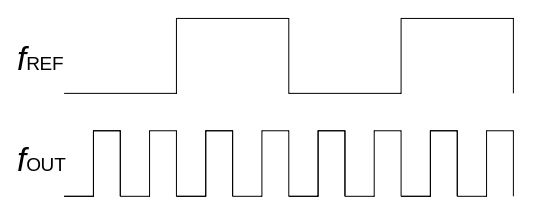
\includegraphics[scale=0.7]{slike/fll_fref_fout.png}
%	 \caption{Демонстарција рада синтетизатора фреквенције за FMUL=4.}
%	 \label{fig:fll:fref_fout}
%\end{figure}
\begin{figure}[!ht]
    \centering
    \vspace{0.5cm}
    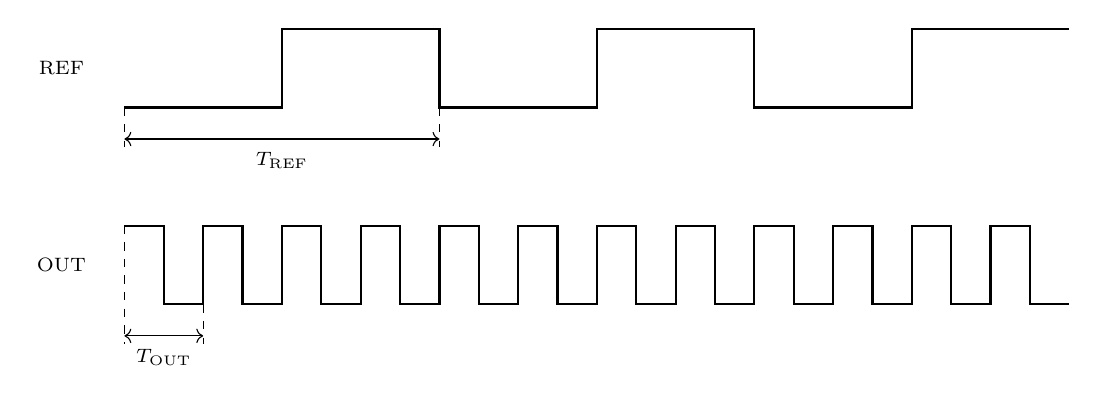
\begin{tikzpicture}

    \def \lref {0}
    \def \href {1}
    \def \lout {-2.5}
    \def \hout {-1.5}

    % Top signal: 3 periods of 4ns
    \draw[thick] (0,\lref) -- (2,\lref) -- (2,\href) -- (4,\href) -- (4,\lref) -- (6,\lref) -- (6,\href) -- (8,\href) -- (8,\lref) -- (10,\lref) -- (10,\href) -- (12,\href);
    \node at (-0.8,0.5) {\scriptsize REF};

    \draw (2,-0.45) node[anchor=north]{\scriptsize $T_\text{REF}$};
    \draw[<->] (0,-0.4) -- (4,-0.4);
    
    % Bottom signal: 12 periods of 1ns
    \draw[thick] (0,\hout) -- (0.5,\hout) -- (0.5,\lout) -- (1,\lout) -- (1,\hout) -- (1.5,\hout) -- (1.5,\lout) -- (2,\lout) -- (2,\hout) -- (2.5, \hout) -- (2.5,\lout) -- (3,\lout) -- (3,\hout) -- (3.5,\hout) -- (3.5,\lout) -- (4,\lout) -- (4,\hout) -- (4.5,\hout) -- (4.5,\lout) -- (5,\lout) -- (5,\hout) -- (5.5,\hout) -- (5.5,\lout) -- (6,\lout) -- (6,\hout) -- (6.5,\hout) -- (6.5,\lout) -- (7,\lout) -- (7,\hout) -- (7.5,\hout) -- (7.5,\lout) -- (8,\lout) -- (8,\hout) -- (8.5,\hout) -- (8.5,\lout) -- (9,\lout) -- (9,\hout) -- (9.5,\hout) -- (9.5,\lout) -- (10,\lout) -- (10,\hout) -- (10.5,\hout) -- (10.5,\lout) -- (11,\lout) -- (11,\hout) -- (11.5,\hout) -- (11.5,\lout) -- (12,\lout);
    \node at (-0.8,-2) {\scriptsize OUT};

    \draw (0.5,-2.95) node[anchor=north]{\scriptsize $T_\text{OUT}$};
    \draw[<->] (0,-2.9) -- (1,-2.9);

    \draw[dashed] (0,\lref) --++ (0,-0.5);
    \draw[dashed] (4,\lref) --++ (0,-0.5);
    \draw[dashed] (0,\hout) --++ (0,-1.5);
    \draw[dashed] (1,\lout) --++ (0,-0.5);
    
    \end{tikzpicture}
    \caption{Демонстрација рада синтетизатора учестаности за FMUL=4.}
    \label{fig:fll:fref_fout}
\end{figure}

\begin{equation}
	f_\text{REF} = \frac{1}{T_\text{REF}}
        \vspace{0.2cm}
\end{equation}
\begin{equation}
	f_\text{OUT} = \frac{1}{T_\text{OUT}}
        \vspace{0.3cm}
\end{equation}
Дефиниција изнад не предвиђа облик синтетисаног излазног сигнала. Он може бити синусоида или правоугаони (дигитални) сигнал, који нам је у CMOS технологији дефинитивно кориснији за разматрање. \par 
У овом раду описана је релативно једноставна али ефикасна дигитална фреквенцијски затворена петља чију системску архитектуру на нивоу блокова приказује \figurename~\ref{FLL block diagram}. Описани \FLL\ се практично састоји из два блока: дигитално контролисаног осцилатора и блока управљачке логике, који генерише улазне сигнале осцилатора на основу тренутне учестаности \DCO-a. У сврху поједностављења, са слике су изостављени неки конфигурациони улази \FLL-a, као што су коефицијенти \PID\ регулатора или улаз за одабир режима рада, чија улога је детаљније описана у поглављу~\ref{Implementation and results}. \par

% FLL block diagram
\begin{figure*}[ht]
	\centering
	\begin{tikzpicture}[thick, scale=0.53, every node/.style={scale=0.45}]
		% Grid
		%\draw[step=1cm, gray, very thin] (0,0) grid (40,10);
		% Setup
		%\tikzset{every node/.style={align=center}};
		%\tikzstyle{every node}=[draw]
		% Beginning
		\draw                         (0  ,0) -- (0  ,5);
		\draw [-]                     (0  ,5) -- (1  ,5);
		\draw [-,  \CtrlColor]        (1  ,5) -- (1.5,5);
		\draw [->, \CtrlPreprocColor] (1.5,5) -- (1.94  ,5);
		% Preprocessing stage (grey counter + gra2bin conversion + synchronization)
		\node (GREYCNT)  at (2.8,5) [draw, \CtrlPreprocColor, minimum size=2cm, minimum height=2.4cm, align=center]{ГРЕЈЕВ  \\ БРОЈАЧ \\[5pt] \framebox{1,3,2,6}};
		\node (CONVSYNC) at (5.8,5) [draw, \CtrlPreprocColor, minimum size=2cm, minimum height=2.4cm, align=center]{СИНХР. \\ БИНАРНИ \\ ПРЕТВАРАЧ \\[5pt] \framebox{$\rightleftarrows$}};
		\draw [->, \CtrlPreprocColor] (GREYCNT) -- (CONVSYNC);
		\draw [dashed, \CtrlPreprocColor, fill=\CtrlPreprocColor, fill opacity=0.1, text opacity=1] (1.5,3.5) rectangle (7.5,6.5) node[midway, above=0.85]{УПРАВЉАЧКА ПРЕДОБРАДА};
		% Splitter/demultiplexer
		\node (DEMUX) at (8.5,5) [draw, \CtrlColor, trapezium, trapezium stretches=true, minimum width=7cm, minimum height=1cm, rotate=90]{ДЕМУЛТИПЛЕКСЕР};
		\draw [-,  \CtrlPreprocColor] (CONVSYNC) -- (7.5,5);
		\draw [->, \CtrlColor]           (7.5,5) -- (DEMUX);
		% Bang-bang FLL control branch
		\draw [-,    \CtrlColor]  (9  ,6.5) -- ( 9.5,6.5);
		\draw [->, \BBctrlColor] ( 9.5,6.5) -- (10  ,6.5);
		\node (CMP) at (11.4,6.5) [draw, \BBctrlColor, minimum size=2cm, minimum height=2.4cm, align=center]{КОМПАРАТОР \\[5pt] \framebox{$\geq$}};
		\node (CNT) at (14.2,6.5) [draw, \BBctrlColor, minimum size=2cm, minimum height=2.4cm, align=center]{БРОЈАЧ \\[5pt] \framebox{1,2,3}};
		\draw [->, \BBctrlColor]      (CMP) --      (CNT);
		\draw [-,  \BBctrlColor]      (CNT) -- (15.5,6.5);
		\draw [->,   \CtrlColor] (15.5,6.5) -- (16  ,6.5);
		\draw [dashed, \BBctrlColor, fill=\BBctrlColor, fill opacity=0.1, text opacity=1] (9.5,5) rectangle (15.5,8) node[midway, above=0.85]{ДВОСТЕПЕНИ РЕГУЛАТОР};
		% PID FLL control branch
		\draw [->, \CtrlColor] ( 9,3.5) -- (11,3.5);
		\node (PID) at (12.5,3.5) [draw, \PIDctrlColor, fill=\PIDctrlColor, fill opacity=0.1, text opacity=1, minimum width=3.5cm, minimum height=2.4cm, align=center]{\PID\ \\ РЕГУЛАТОР \\[5pt]};
		\draw [\PIDctrlColor] plot[smooth] coordinates {(11.75,2.7) (12.0,3.2) (12.5,3.1) (13.25,3.1)};
		\draw [\PIDctrlColor, fill=\PIDctrlColor, fill opacity=0.1] (11,2.5) rectangle (14,4.5) node[midway, below=0.6, opacity=1] {};
		\draw [->, \CtrlColor] (14,3.5) -- (16,3.5);
		% Control logic box
		\draw [dashed, \CtrlColor, fill=\CtrlColor, fill opacity=0.1, text opacity=1] (1,1) rectangle (21,9) node[midway, above=2.15]{УПРАВЉАЧКА ЛОГИКА};
		% Multiplexer
		\node (MUX) at (16.5,5) [draw, \CtrlColor, trapezium, trapezium stretches=true, minimum width=7cm, minimum height=1cm, rotate=-90]{МУЛТИПЛЕКСЕР};
		% Control Decoder
		\node (CTRLDEC) at (19,5) [draw, \CtrlDecColor, fill=\CtrlDecColor, fill opacity=0.1, text opacity=1, minimum size=2cm, minimum height=2.4cm, align=center]{УПРАВЉАЧКИ \\ ДЕКОДЕР};
		\draw [->, \CtrlColor] (MUX)  -- (CTRLDEC);
		% DCO
		\node (DCO) at (23,5) [draw, \DCOColor, fill=\DCOColor, fill opacity=0.1, text opacity=1, minimum size=2.4cm, minimum height=2.4cm, align=center]{DCO \\[5pt]};
		\draw [\DCOColor](22.8,4.7) sin (22.9,4.8) cos (23.0,4.7) sin (23.1,4.6) cos (23.2,4.7);
		\draw [\DCOColor](23.0,4.7) circle (0.3);
		\draw [-, \CtrlColor] (CTRLDEC) -- (21,5);
		\draw [->]                     (21,5) --  (DCO);
		% End
		\draw  (DCO) -- (25,5);
		\draw (25,5) -- (25,0);
		\draw (25,0) --  (0,0);
		
        \draw (-1,-1) rectangle (26,10) node[midway, above=2.95]{\textbf{ДИГИТАЛНА ФРЕКВЕНЦИЈСКИ ЗАТВОРЕНА ПЕТЉА}};	
        \draw [thick, ->] (-2.5,9) -- (-1,9) node[midway, above=0.1] {\textbf{RSTN}};
        \draw [thick, ->] (-2.5,8) -- (-1,8) node[midway, above=0.1] {\textbf{FREF}};        	
        \draw [thick, ->] (-2.5,7) -- (-1,7) node[midway, above=0.1] {\textbf{FMUL}};
        \draw [thick, ->] (-2.5,6) -- (-1,6) node[midway, above=0.1] {\textbf{CTRL}};
        \draw (-2.0,6.825) --  (-1.5,7.175);
        \draw (-2.0,5.825) --  (-1.5,6.175);
        %\draw [-]  (25,5) -- (26,5);
        \draw [thick, ->] (26,8) -- (27.5,8) node[midway, above=0.1] {\textbf{FOUT}};
        \draw [thick, ->] (26,7) -- (27.5,7) node[midway, above=0.1] {\textbf{LOCK}};
        
		
	\end{tikzpicture}
	\caption{Блок дијаграм дигиталне фреквенцијски затворене петље састављене од: блока управљачке логике (лијево) и дигитално контролисаног осцилатора (десно).}
	\label{FLL block diagram}
\end{figure*}

\vspace{0.7cm} % go to next page
Основни улази у систем су:
\begin{itemize}
	\item RSTN - Ресет сигнал који је активан на нулу,
	\item FREF - Референтни такт,
	\item FMUL - Улазни умножак учестаности (множењем са учестаношћу референтног такта добија се вриједност учестаности коју треба постићи и одржавати на излазу),
	\item CTRL - Сигнал који одређује који од два управљачка режима се користи.
\end{itemize}
Излази из система су:
\begin{itemize}
	\item FOUT - Излазни такт,
	\item LOCK - Сигнал који говори да ли је систем ушао у стабилно стање тј. да ли ради на жељеној учестаности.
\end{itemize}

\section{Управљачка логика дигиталне фреквенцијски затворене петље} \label{section:ctrl}
Управљачка логика \FLL-a састоји се од двије независне процесне гране, које представљају два међусобно искључива режима управљања \FLL-a. Оба режима на улазу примају бинарну вриједност која представља број периода такта \DCO-а унутар периода референтног такта. Такође, оба управљачка режима генеришу бинарну вриједност на излазу, која представља управљачку бинарну ријеч осцилатора директно пропорционалну учестаности излазног сигнала. Главне разлике између два поменута режима су брзина затварања (закључавања) \FLL-a и једноставност подешавања. Циљ управљачке логике \FLL-a је изједначити вриједност улазног множача учестаности са бројем периода такта \DCO-a унутар периода референтног такта што је брже и прецизније могуће, чиме се долази до постизања жељене учестаности на излазу \DCO-a. Поред самог постизања жељене учестаности, задатак управљачке логике је и њено одржавање током времена јер, због утицаја разних фактора, као што је нпр. температура, константно долази до нежељеног смањења или повећања вриједности учестаности. То значи да управљачка логика константно прати рад система и по потреби реагује на исход непожељних утицаја на излазну учестаност. Комплетна управљачка логика \FLL-a је подијељена на неколико фаза, које су детаљно описане у наредним поглављима, а то су:
\begin{itemize}
	\item Управљачка предобрада
	\item Двостепени регулатор / \PID\ регулатор
	\item Управљачки декодер
\end{itemize}

\subsection{Управљачка предобрада} \label{section:control_preprocessing}
Фаза управљачке предобраде \engl{Control Preprocessing} укључује неколико блокова чија је улога претворити информацију о учестаности излазног такта \DCO-a у бинарну вриједност која ће бити прослијеђена као улаз наредној фази управљачке логике \FLL-a. Као прво, да би се одредила брзина осциловања \DCO-a, потребан је бројач. У имплементацији описаној у овом раду коришћен је Грејев бројач. У Грејевом коду свака узастопна вриједност се разликује за само један бит. То му даје предност у односу на природни бинарни бројач из разлога што значајно умањује метастабилност бројача изазвану узорковањем \engl{Sampling} вриједности бројача. \tablename~\ref{gray_code} приказује првих осам цифара у Грејевом коду, у поређењу са природним бинарним цифрама. \par
\begin{table}[!ht]
	\caption{Првих осам цифара у Грејевом коду}
	\label{gray_code}
	\centering
	\begin{tabular}{|c|c|c|c|}
		\hline
		Децимални запис & Бинарни запис & Грејев код & Грејев код у децималном запису \\
		\specialrule{1pt}{0pt}{0pt}
		0 & 000 & 000 & 0 \\
		\hline
		1 & 001 & 001 & 1 \\
		\hline
		2 & 010 & 011 & 3 \\
		\hline
		3 & 011 & 010 & 2 \\
		\hline
		4 & 100 & 110 & 6 \\
		\hline
		5 & 101 & 111 & 7 \\
		\hline
		6 & 110 & 101 & 5 \\
		\hline
		7 & 111 & 100 & 4 \\
		\hline
	\end{tabular}
\end{table}
Као примјер појаве метастабилности може се навести проблем који се може јавити у употреби природних бинарних кодова, а то је да се, при преласку у наредно стање бројача, стање свих битова који се мијењају не мора промијенити тачно синхронизовано. Рецимо, при преласку из стања 3 у стање 4 (бинарно 011 у 100), код природног бинарног бројача сви битови мијењају стање, тако да та транзиција може да иде редом 011 $\rightarrow$ 001 $\rightarrow$ 101 $\rightarrow$ 100, што значи да могу да постоје два прелазна стања, која могу бити прочитана чиме би коначно стање бројача било погрешно. У овом конкретном случају, умјесто у стање 4 (бинарно 100), бројач би завршио у стању 1 (бинарно 001) или 5 (бинарно 101), за шта не постоји могућност при употреби Грејевог кода јер се у њему из стања 011 прелази у стање 010, при чему се мијења само један бит. Треба напоменути да могућност појаве метастабилности и даље постоји јер је то много општија појава иза проблема погрешног узорковања у случају када се у исто вријеме мијењају такт и подаци, али Грејев код омогућује да се потенцијална грешка сведе на максимално један бит. \par 
Недостатак овог приступа је то што имплементација Грејевог бројача из овог рада има мању максималну радну учестаност од природног бинарног бројача. Да би се значајно више смањио ризик од метастабилности, сваки бит са излаза Грејевог бројача се пропушта кроз синхронизатор са два флип-флопа да би безбједно прешао у подручје референтног такта. Затим, синхронизована вриједност Грејевог бројача се претвара у природан бинарни формат и узоркује се за даљу обраду.

\subsection{Двостепени регулатор} \label{section:bang_bang}
У теорији управљања, двостепени регулатор (двофазни, bang-bang или on-off регулатор) је регулатор повратне спреге које се нагло пребацује између два стања. Математички модел двостепеног регулатора може се представити преко Хевисајдове функције (или јединичне одскочне функције) која се иначе користи у математици система управљања и обради сигнала да би се представио сигнал који мијења стање у одређено вријеме. Она има вриједност $0$ за негативне вриједности аргумента и $1$ за позитивне вриједности аргумента:
% TODO
% Пребацити у TikZ слику испод
%\begin{figure}[!h]
%	 \centering
%	 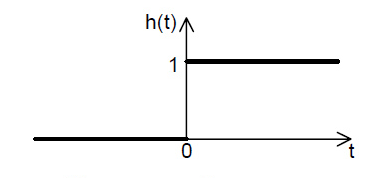
\includegraphics[scale=0.7]{slike/heaviside.png}
%	 \caption{График Хевисајдове функције.}
%	 \label{heaviside}
%\end{figure}
\begin{figure}[!ht]
    \centering
    \resizebox{7cm}{5cm}{%
    \begin{tikzpicture}
    \begin{axis}[
        axis lines=middle,
        xlabel={$x$},
        ylabel={$u(x)$},
        ymin=-0.1, ymax=1.1,
        xmin=-4, xmax=4,
        xtick={0},
        ytick={0,1},
        every axis x label/.style={
            at={(current axis.right of origin)}, anchor=west,
        },
        every axis y label/.style={
            at={(current axis.above origin)}, anchor=south,
        },
        ]
        \addplot[domain=-4:0,very thick,samples=2] {0}; % Plot for x < 0
        \addplot[domain=0:4,very thick,samples=2] {1}; % Plot for x > 0
        
        % Draw a vertical dashed line at x = 0
        \draw[dashed,very thick] (axis cs:0,0) -- (axis cs:0,1);
        
        % Optional: add open circle at (0,0)
        %\addplot[thick,only marks,mark=*,mark options={fill=white}] coordinates {(0,0)};
        % Optional: add filled circle at (0,1)
        %\addplot[thick,only marks,mark=*] coordinates {(0,1)};
    \end{axis}
    \end{tikzpicture}
    }
    \caption{График јединичне одскочне функције.}
    \label{heaviside}
\end{figure}

\begin{equation}
	\label{eq_heaviside}
	u(x)= \begin{cases}
		0, & x < 0 \\
		1, & x > 0
		\end{cases}
\end{equation}
Главне предности примјене двостепеног регулатора су једноставна имплементација и брз одговор на промјене, док су недостаци могуће осцилације око жељене вриједности након што се она постигне, као и непогодност за системе гдје је потребно веома прецизно управљање. \par 
Kao што је већ наведено, \FLL\ из овог рада има два међусобно искључива управљачка блока. Један управљачки блок \FLL-a је веома сличан двостепеном регулатору описаном изнад. Он пореди улазни умножак учестаности са узоркованом вриједношћу бројача и одлучује да ли инкрементирати, декрементирати или онемогућити предстојећи блок тј. двосмјерни бројач \engl{Up-Down Counter}. Ако је улазни умножак учестаности већи од вриједности бројача узорковане у блоку управљачке предобраде, тада се двосмјерни бројач инкрементира, ако је мањи тада се декрементира, а у случају да је једнак, двосмјерни бројач задржава претходно стање. То осигурава постепено управљање и закључавање све до постизања жељене учестаности тј. преласка у стабилно стање. Како би се спријечиле (или барем прориједиле) могуће осцилације око жељене вриједности, у овом блоку је доведен додатни сигнал који омогућава да се, након што систем једном уђе у стабилно стање, бројач двостепеног регулатора не инкрементира или декрементира баш након сваког одступања од жељене вриједности јер се очекује да у стабилном стању та одступања буду незнатна. Тај додатни сигнал се користи и у \PID\ регулатору који представља други управљачки режим о коме ће више ријечи бити у наредном поглављу.

\subsection{\PID\ регулатор} \label{section:pid}
У другом управљачком режиму, управљачка бинарна ријеч за \DCO\ се генерише подесивим \PID\ регулатором. \PID\ регулатор је далеко најчешће коришћен алгоритам за управљање у инжењерству. Највећим бројем повратних спрега се управља преко \PID\ регулатора или његових дјелимичних варијација~\cite{Astrom:PID_1995}. \PID\ регулатор је управљачки механизам заснован на повратној спрези, који ради тако што непрекидно исправља и скалира сигнал грешке. Грешка у овом случају представља разлику између измјерене вриједности у управљачкој предобради (узоркована вриједност бројача) и жељене референтне задате вриједности (вриједност улазног умношка учестаности). Исправљање и скалирање се распоређује у три компоненте које су имплементиране помоћу подесивих коефицијената, цијелих бројева у бинарном формату са фиксном тачком, добијених из регистарске банке: 
\begin{itemize}
	\item Пропорционална (\P) - управља брзином одзива управљачког системам непосредно множећи сигнал грешке константним чиниоцем који се назива и константа пропорционалног појачања. Ако је она превелика, систем може постати нестабилан. Насупрот томе, њена премала вриједност доводи до малог излазног одзива на велику улазну грешку чиме регулатор постаје мање осјетљив. 
	\item Интегрална (\I) - користи се за смањење грешке стабилног стања \engl{Steady State} скалирањем грешке константним чиниоцем и сумирањем резултата током времена. Грешка стабилног стања је разлика између жељене и стварне вриједности коначног излаза~\cite{Liptak:PROCESS_CONTROL_2006}. Интегрално дејство убрзава кретање излаза ка жељеној вриједности.
	\item Диференцијална (\D) - пропорционална брзини промјене грешке, и њен циљ је ограничити излаз да би се смањила могућа прекорачења или осцилације узроковане \P\ и \I\ компонентама, без смањења брзине регулатора. Како је у овом систему референтна задата вриједност константна и нема брзих промјена на улазу које могу изазвати такав исход, \P\ и \I\ компоненте су довољне за гладак и стабилан одзив система. \par
\end{itemize}
Математички, цјелокупна управљачка функција \PID\ регулатора представља суму пропорционалног, интегралног и диференцијалног дејства и записује се на следећи начин:
\begin{equation} 
	\label{eq_pid_1}
	y(t)= K_\text{p}e(t) + K_\text{i}\int_{0}^{t}e(\tau)d\tau + K_\text{d}\frac{de(t)}{dt},
\end{equation}
гдје су $K_\text{p}$, $K_\text{i}$ и $K_\text{d}$ коефицијенти за пропорционални, интегрални и диференцијални дио, респективно. У стандардном облику, једначина~\ref{eq_pid_1} се записује као
\begin{equation} 
	\label{eq_pid_2}
	y(t)= K_\text{p}\left(e(t) + \frac{1}{T_\text{i}}\int_{0}^{t}e(\tau)d\tau + T_\text{d}\frac{de(t)}{dt}\right).
\end{equation}
Као што се може видјети, коефицијенти $K_\text{i}$ и $K_\text{d}$ су редом замјењени са $K_\text{p}/T_\text{i}$ и $K_\text{p}T_\text{d}$, а предност таквог записа јесте што $T_\text{i}$ и $T_\text{d}$ имају одређено разумљиво физичко значење, јер представљају интегрално и диференцијално вријеме, респективно. $K_\text{p}/T_\text{i}$ одређује колико временски дуго ће регулатор толерисати излаз који се налази изнад или испод жељене вриједности. $K_\text{p}T_\text{d}$ је временска константа којом се регулатор покушава приближити жељеној вриједности. \par
% TODO
% Пребацити у TikZ слику испод
%\begin{figure}[!h]
%	 \centering
%	 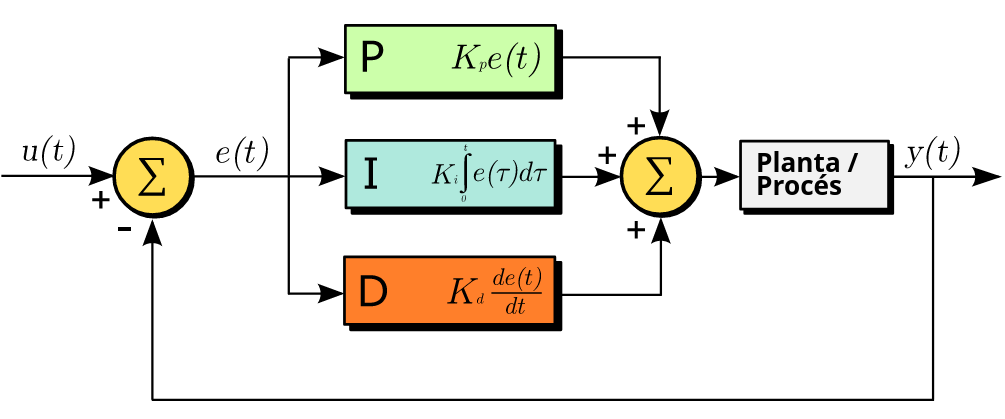
\includegraphics[scale=0.3]{slike/pid.png}
%	 \caption{Блок дијаграм \PID\ регулатора у повратној спрези.}
%	 \label{pid_img}
%\end{figure}
\begin{figure}[!ht]
    \centering
    %\vspace{0.5cm}
    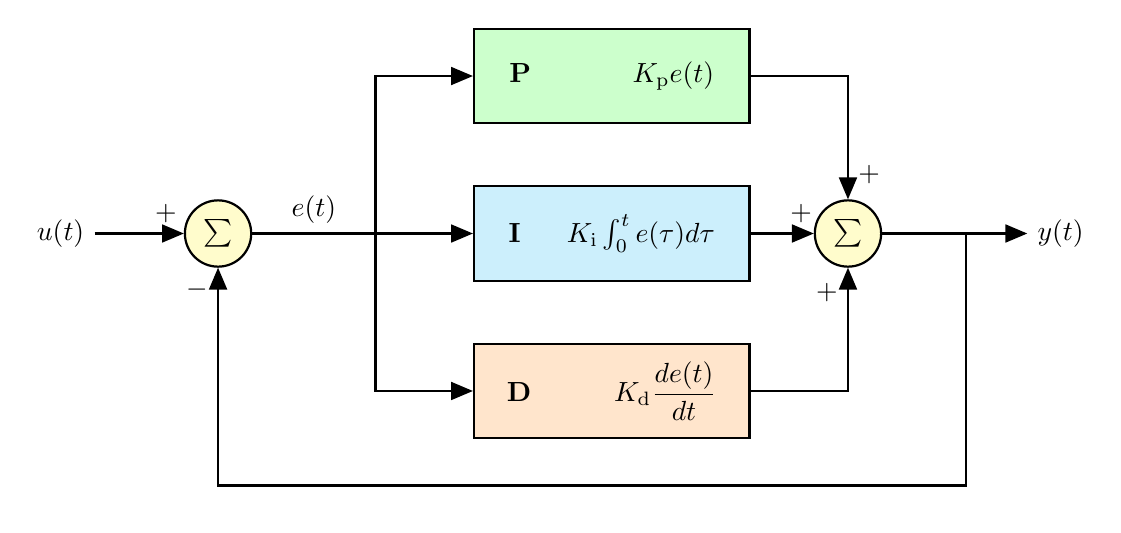
\begin{tikzpicture}[auto, thick, node distance=2cm, >=triangle 45]
    % Nodes
    \node [draw, circle, fill=yellow!20] (sum1) {$\sum$};
    \node [left of=sum1, node distance=2cm] (input) {$u(t)$};
    \node [right of=sum1] (e) {};
    \node [draw, rectangle, minimum width=3.5cm, minimum height=1.2cm, fill=cyan!20, right of=e, node distance=3cm] (I) {\textbf{I}\ \ \ \ \ $K_\text{i} \int_0^t e(\tau) d\tau$};
    \node [draw, rectangle, minimum width=3.5cm, minimum height=1.2cm, fill=green!20, above of=I, node distance=2cm] (P) {\textbf{P}\ \ \ \ \ \ \ \ \ \ \ $K_\text{p} e(t)$};
    \node [draw, rectangle, minimum width=3.5cm, minimum height=1.2cm, fill=orange!20, below of=I, node distance=2cm] (D) {\textbf{D}\ \ \ \ \ \ \ \ \ $K_\text{d} \dfrac{de(t)}{dt}$};
    \node [draw, circle, fill=yellow!20, right of=I, node distance=3cm] (sum2) {$\sum$};
    % \node [draw, rectangle, right of=sum2, node distance=2cm] (plant) {Обрада};
    \node [right of=sum2, node distance=1.5cm] (output) {};
    \node [right of=output, node distance=1.2cm] (yout) {$y(t)$};

    % Arrows
    \draw[->] (input) -- node [pos=0.8] {$+$} (sum1);
    \draw[-] (sum1) -- node {$e(t)$} (e.center);
    \draw[->] (e.center) |- (P);
    \draw[->] (P) -| node [pos=0.9] {$+$} (sum2);
    \draw[->] (e.center) -- (I);
    \draw[->] (I) -- node [pos=0.8] {$+$} (sum2);
    \draw[->] (e.center) |- (D);
    \draw[->] (D) -| node [pos=0.9] {$+$} (sum2);
    \draw[-] (sum2) -- (output.center);
    % \draw[-] (plant) -- (output.center);
    \draw[->] (output.center) -- (yout);
    \draw[->] (output.center) |- ++(0,-3.2) -| node[pos=0.05] {} node[pos=0.95] {$-$} (sum1);

    \end{tikzpicture}   
    %\vspace{0.5cm}
    \caption{Блок дијаграм \PID\ контролера у повратној спрези.}
    \label{pid_img}
\end{figure}

\figurename~\ref{pid_img} представља уопштен блок дијаграм \PID\ регулатора у повратној спрези који приказује структуру компоненти регулатора и њихов принцип рада. \PID\ регулатор константно рачуна вриједност грешке $e(t)$ као разлику између жељене вриједности \engl{Setpoint} $u(t)$, која у овом конкретном случају представља улазни умножак учестаности, и измјерене процесне вриједности $y(t)$, односно вриједности измјерене у блоку управљачке предобраде. У том случају, једначина грешке може се записати као
\begin{equation} 
	\label{eq_pid_err)}
	e(t) = u(t) - y(t).
\end{equation}
Одзив система тј. брзина и начин достизања жељене учестаности у \PID\ режиму рада највише зависи од одабира константи регулатора, а у овом раду је остављена могућност софтверског уписа константи у регистре, што даље омогућава њихово накнадно мијењање и прилагођавање. У поглављу~\ref{section:python_model}, гдје је приказан софтверски модел понашања \FLL-a имплементиран у Пајтон програмском језику, поред осталог је дат и сликовит приказ утицаја константи \PID\ регулатора на одзив система.

\subsection{Управљачки декодер} \label{section:control_decoder}
Улога управљачког декодера је претворити управљачке податке из једне бинарне вриједности у скуп управљачких улаза \DCO-а. Постоје три таква улаза: \textit{Row On}, унарни вектор, који може да укључује само читаве редове тростатичких инвертора \DCO-a; \textit{Row Select}, један од $n$ \engl{One-Hot} вектор, који укључује један додатни ред тростатичких инвертора \DCO-a; и \textit{Column Select}, унарни вектор, који може да укључује колоне тростатичких инвертора \DCO-a. \par
Један од $n$ вектор представља групу битова гдје је једина исправна комбинација она са једном јединицом и свим осталим нулама~\cite{Harris:DIGITAL_DESIGN_2012}. При представљању неког природног броја као један од $n$ вектора, вриједност броја је једнака позицији јединице у вектору. С друге стране, да би се природан број $N$ представио као унарни вектор, јединица се понавља $N$ пута узастопно~\cite{Davis:COMPUTABILITY_1994}. \tablename~\ref{one_hot_unary} приказује примјер представљања природних бројева у унарном и један од $n$ запису. \par
\begin{table}[!ht]
	\caption{Поређење унарног и један од $n$ записа}
	\label{one_hot_unary}
	\centering
	\begin{tabular}{|c|c|c|c|}
		\hline
		Децимални & Бинарни & Унарни & Један од $n$ \\
		\specialrule{1pt}{0pt}{0pt}
		0 & 000 & 00000000 & 00000001 \\
		\hline
		1 & 001 & 00000001 & 00000010 \\
		\hline
		2 & 010 & 00000011 & 00000100 \\
		\hline
		3 & 011 & 00000111 & 00001000 \\
		\hline
		4 & 100 & 00001111 & 00010000 \\
		\hline
		5 & 101 & 00011111 & 00100000 \\
		\hline
		6 & 110 & 00111111 & 01000000 \\
		\hline
		7 & 111 & 01111111 & 10000000 \\
		\hline
	\end{tabular}
\end{table}
Да би се инвертор укључио, или \textit{Row On}, или и \textit{Row Select} и \textit{Column Select} за одговарајући бит морају бити подешени на 1 (једначина~\ref{dco_cell_ctrl_eq}). Ширина сваког вектора је једнака ширини улаза \DCO-а. Структура \DCO-a је детаљно описана у поглављу \ref{DCO chapter}. \par 
Управљачки податак који долази из претходног степена тј. контолера представља број тростатичких инвертора \DCO-а који требају бити укључени, и што их је више укључено, то је излазна учестаност већа. Рецимо да је тај број 50, и претпоставимо да је \DCO\ састављен од 255 тростатичких инвертора које поједностављено можемо посматрати као прекидаче и нека су организовани у 17 редова и 15 колона. Како постоји 17 редова, ширине \textit{Row On} и \textit{Row Select} вектора биће по 17 битова, док ће због 15 колона, ширина \textit{Column Select} вектора бити 15 битова. То значи, да би се укључило 50 прекидача, потребно је укључити 3 читава реда прекидача и још 5 прекидача из четвртог реда. Да би се то постигло, управљчки улази \DCO-а морају имати следеће вриједности:
\begin{itemize}
	\item \textit{Row On} = $00000000000000111$ $\rightarrow$ Сви прекидачи у три прва реда су укључени. 
	\item \textit{Row Select} = $00000000000001000$ $\rightarrow$ У четвртом реду је укључено још инвертора.
	\item \textit{Column Select} = $000000000011111$ $\rightarrow$ Пет инвертора је укључено у реду који је одређен са \textit{Row Select}.
\end{itemize}

\section{Теоријско разматрање осцилатора} \label{Oscillation basics}
У срцу сваке фазно затворене петље се налази осцилатор који игра кључну улогу у учинку који може бити постигнут~\cite{Razavi:PLL_CMOS_2020}. Имајући то у виду, у наставку ће кроз теорију и примјере бити описани основни концепти осциловања, а након тога се прелази на разматрање концепта дигитално контролисаног осцилатора. \par

\subsection{Основни принципи осциловања}
У сврху теоријског разматрања осцилатора, као примјер биће узето клатно, као на Слици~\ref{pendulum}. \par
\begin{figure}[!ht]
    \centering
    \vspace{0.5cm}
    \begin{tikzpicture}

	% Position 1
	\node at (0, 0) {};
	\draw[thick] (0,0) -- (-2,-2);
	\draw[dashed] (0,0) -- (0,-2.84);
	\draw[fill=white] (0,0) circle (2pt);
	\draw[fill=white, thick] (-2,-2) circle (6pt);
	\node[align=center] at (-2,-2.8) {потенцијална\\енергија};
	\node at (0,0.5) {положај 1};

	% Position 2
	\begin{scope}[shift={(3,0)}]
	\draw[thick] (0,0) -- (0,-3);
	\draw[fill=white] (0,0) circle (2pt);
	\draw[fill=white, thick] (0,-3) circle (6pt);
	\node[align=center] at (1.2,-2.7) {кинетичка\\енергија};
	\draw[<-,thick] (1,-3.5) arc[start angle=-60, end angle=-120, radius=2];
	\node at (0,0.5) {положај 2};
	\end{scope}

	% Position 3
	\begin{scope}[shift={(6,0)}]
	\draw[thick] (0,0) -- (2,-2);
	\draw[dashed] (0,0) -- (0,-2.84);
	\draw[fill=white] (0,0) circle (2pt);
	\draw[fill=white, thick] (2,-2) circle (6pt);
	\node[align=center] at (2.2,-2.8) {потенцијална\\енергија};
	\node at (0,0.5) {положај 3};
	\end{scope}

    \end{tikzpicture}
    %\vspace{0.5cm}
    \caption{Клатно које дјелује као осцилаторни систем~\cite{Razavi:PLL_CMOS_2020}.}
    \label{pendulum}
\end{figure}

Ако пустимо клатно под одређеним углом, оно се неко вријеме њише и постепено се зауставља. Осцилација почиње јер се првобитна потенцијална енергија претвара у кинетичку енергију како клатно достиже свој вертикални положај, дозвољавајући му да настави своју путању до другог екстремног угла (положај 3), под којим је енергија поново у потенцијалном облику. У реалним условима осцилација престаје јер трење на оси око које се окреће клатно и отпор ваздуха претварају дио енергије клатна у топлоту у сваком периоду осциловања. \par
Да би се одржала осцилација, потребно је обезбиједити спољну енергију клатну, како би се надомјестио губитак изазван трењем на оси и отпором ваздуха. Рецимо ако се лагано гурне клатно сваки пут када се врати у положај 1, оно ће настављати да се њише. Ако је притисак сувише слаб, врши се недовољна компензација, чиме се дозвољава осцилацији да ослаби и временом нестане. С друге стране, ако је притисак прејак, врши се прекомјерна компензација, приморавајући амплитуду замаха да се повећава из једног циклуса у други. Такође, треба напоменути да је период осциловања независан од амплитуде осциловања~\cite{Razavi:PLL_CMOS_2020}. \par
Механички примјер изнад указује на неколико саставних дијелова осцилаторног система:
\begin{enumerate}
	\item Почетна „неравнотежа“, тј. почетно стање или количина енергије (обезбијеђена довођењем клатна у положај 1).
	\item Склоност да се једна врста енергије претвара у другу и обрнуто.
	\item Механизам за одржавање који допуњује енергију изгубљену усљед неизбјежних несавршености.
\end{enumerate}
Не садрже сви осцилаторни системи све поменуте саставне дијелове, али је корисно имати ове концепте на уму при разматрању неког система који осцилује. \par
Ако се идеално клатно (клатно без губитака) пусти под одређеним углом, такво клатно осцилује бесконачно. Ако се дода одређени притисак сваки пут када клатно дође до лијевог краја, тада замах наставља да расте због додатне енергије која се уноси у систем у сваком циклусу. Треба имати на уму да се тај неограничени раст не дешава ако се додатни притисак унесе на учестаности различитој од природне учестаности осциловања клатна. Ако систем има склоност да осцилује на учестаности $\omega_{0}$, тада се ствара растући осцилаторни излаз као одговор на спољашњу побуду на учестаности $\omega_{0}$. Из друге перспективе, такав систем неограничено појачава периодични улаз на поменутој учестаности.

\subsection{Систем осцилаторне повратне спреге}
Из основа аутоматског управљања се зна да систем са негативном повратном спрегом може постати нестабилан. Ово својство се користи за конструисање осцилатора. \par
У сврху проучавања осцилација у фреквенцијском домену, разматрамо систем повратне спреге приказан на Слици~\ref{osc_feedback_1}, гдје негативан предзнак на једном улазу сабирача означава негативну повратну спрегу на ниским учестаностима. На Слици~\ref{osc_feedback_2} је приказан примјер имплементације такве повратне спреге, који, на нискофреквентни синусоидни улаз дјелује као јединични бафер. Треба имати на уму да операциони појачавач показује занемарљив фазни помак на ниским учестаностима. \par
% TODO
% Пребацити у TikZ слике
%\begin{figure}[!ht]
%	 \centering
%	 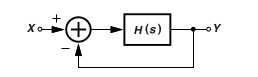
\includegraphics[scale=0.8]{slike/osc_feedback_1.png}
%	 \caption{Једноставан систем повратне спреге.}
%	 \label{osc_feedback_1}
%\end{figure}
\begin{figure}[!ht]
    \centering
    \vspace{0.5cm}
    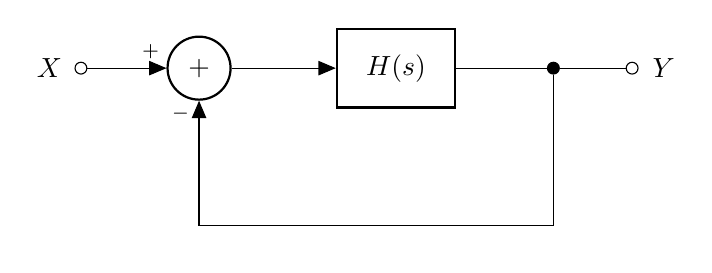
\begin{tikzpicture}[auto, >=triangle 45]
    
    %\node at (0, 0) {};
    \node [draw, circle, thick, minimum size=0.8cm, inner sep=0] (sum) {$+$};
    \node [draw, circle, minimum size=0.15cm, left of=sum, inner sep=0, node distance=1.5cm] (circx) {};
    %\node [draw, circle, thick, minimum size=0.5cm, right of=sum, node distance=2cm, inner sep=0] (circvn) {};
    \node [draw, rectangle, thick, minimum width=1.5cm, minimum height=1cm, right of=sum, node distance=2.5cm] (block) {$H(s)$};
    \node [draw, circle, minimum size=0.15cm, inner sep=0,  fill=black, right of=block, node distance=2cm] (out) {};
    %\node [draw, ground, below left of=sum, node distance=2cm] (gnd) {};
    \node [draw, circle, minimum size=0.15cm, right of=out, inner sep=0] (circy) {};
    %\node [above of=circvn, node distance=0.6cm] {$V_{n}$};
    \node [right of=circy, node distance=0.4cm] {$Y$};
    \node [left of=circx, node distance=0.4cm] {$X$};

    %\draw (-1.6,0) sin (-1.5,0.2) cos (-1.4,0) sin (-1.3,-0.2) cos (-1.2,0);
    %\draw (0.7,0.6) sin (0.8,1) cos (0.9,0.6) sin (1.0,0.2) cos (1.1,0.6);
    %\draw (-0.5,-1) sin (-0.4,-1.2) cos (-0.3,-1) sin (-0.2,-0.8) cos (-0.1,-1);

    \draw[->] (circx) -- node [pos=0.8] {\scriptsize $+$} (sum);
    %\draw[->] (circin) -- node [pos=0.7] {\scriptsize $+$} (sum);
    %\draw[->] (gnd) -- node [pos=0.7] {\scriptsize $-$} (sum1);
    \draw[->] (sum) -- (block);
    %\draw[->] (circvn) -- node [pos=0.1] {\scriptsize $+$} node [pos=0.5, below of=circvn, node distance=0.3cm] {$P$} (block);
    \draw[->] (block) -- (out) |- ++(0,-2) -| node[pos=0.05] {} node[pos=0.95] {\scriptsize $-$} (sum);
    \draw[-] (out) -- (circy);
    \end{tikzpicture}
    %\vspace{0.5cm}
    \caption{Једноставан систем повратне спреге.}
    \label{osc_feedback_1}
\end{figure}

%\begin{figure}[!ht]
%	 \centering
%	 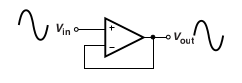
\includegraphics[scale=0.8]{slike/osc_feedback_2.png}
% 	 \caption{Реализација повратне спреге коришћењем операционог појачавача.}
%	 \label{osc_feedback_2}
%\end{figure}
\begin{figure}[!ht]
    \centering
    \vspace{0.5cm}
    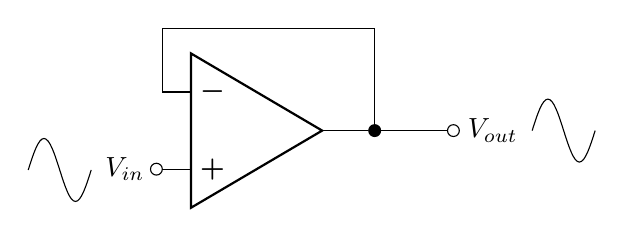
\begin{tikzpicture}[auto, >=triangle 45]
    
    % Op-Amp
    \draw (0,0) node[op amp] (opamp) {};

    \node [draw, circle, minimum size=0.15cm, inner sep=0,  fill=black, right of=opamp, node distance=1.5cm] (out) {};
    \node [draw, circle, minimum size=0.15cm, right of=out, inner sep=0] (circvout) {};
    
    \draw (opamp.+) node[draw, left, circle, minimum size=0.15cm, inner sep=0, node distance=2cm] (circvin) {};
    \node [left of=circvin, node distance=0.4cm] (vin) {$V_{in}$};
    \node [right of=circvout, node distance=0.5cm] (vout) {$V_{out}$};
    \draw (opamp.out) -- (out) -- (circvout);
    \draw (out) |- ++(0,1.3) -| (opamp.-);
    
    \draw (-2.9,-0.5) sin (-2.7,-0.1) cos (-2.5,-0.5) sin (-2.3,-0.9) cos (-2.1,-0.5);
    \draw (3.5,0) sin (3.7,0.4) cos (3.9,0) sin (4.1,-0.4) cos (4.3,0);

    \end{tikzpicture}
    %\vspace{0.5cm}
    \caption{Реализација повратне спреге коришћењем операционог појачавача.}
    \label{osc_feedback_2}
\end{figure}

Међутим, поставља се питање како могу системи са Слика~\ref{osc_feedback_1}~и~\ref{osc_feedback_2} да осцилују? Записивањем преносне функције затворене петље као 
\begin{equation} 
	\label{transfer_function}
	\frac{Y(s)}{X(s)}=\frac{H(s)}{1+H(s)},
\end{equation}
примјећује се да именилац пада на нулу ако је $H(s)=-1$ за неку вриједност промјенљиве $s$. Ако је $X(s)$ синусоида, онда је $s=j\omega_{0}$ и мора важити $H(j\omega_{0})=-1$. С обзиром да је у питању синусоида, то ће на $\omega_{0}$ важити за фазни помјерај од $-180^{\circ}$. То даље значи да важи $(Y/X)(j\omega_{0}) \rightarrow \pm\infty$, одакле се може закључити да систем обезбјеђује неограничен добитак за такву синусоиду. Као што је претпостављено у претходним поглављу, такво понашање наговјештава осцилаторну петљу. \par
Једнакост $H(j\omega_{0})=-1$ значи да $H(s)$ инвертује улаз на учестаности $\omega_{0}$, што је илустровано на Слици~\ref{osc_feedback_3}. Другим ријечима, $H(s)$ има толико помјерања фазе (или кашњења) на $\omega_{0}$ да укупна повратна спрега постаје позитивна. То се може видјети постављањем главног улаза, $X(s)$, на нулу, прекидом петље и примјеном стимулуса на истој учестаности (\figurename~\ref{osc_feedback_4}). Враћени сигнал је у фази са испитним напоном, $V_{t}$. У овом случају, каже се да петља садржи фазни помјерај од $180^{\circ}$ због номинално негативне повратне спреге и други, фреквенцијски зависан, фазни помјерај од $180^{\circ}$ који произилази из $H(s)$. Та два фазна помјераја се не смију мијешати један с другим. \par
%\begin{figure}[!ht]
%	 \centering
%	 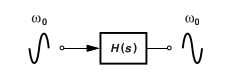
\includegraphics[scale=0.8]{slike/osc_feedback_3.png}
%	 \caption{Инверзија сигнала на фреквенцији $\omega_{0}$.}
%	 \label{osc_feedback_3}
%\end{figure}
\begin{figure}[!ht]
    \centering
    \vspace{0.5cm}
    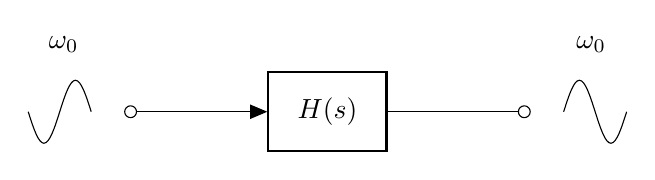
\begin{tikzpicture}[auto, >=triangle 45]
    
    \node [draw, rectangle, thick, minimum width=1.5cm, minimum height=1cm] (block) {$H(s)$};
    \node [draw, circle, minimum size=0.15cm, left of=block, inner sep=0, node distance=2.5cm] (circin) {};
    \node [draw, circle, minimum size=0.15cm, right of=block, inner sep=0, node distance=2.5cm] (circout) {};
    
    \node [above left of=circin, node distance=1.2cm] (omegain) {$\omega_{0}$};
    \node [above right of=circout, node distance=1.2cm] (omegaout) {$\omega_{0}$};

    \draw (-3.8,0) sin (-3.6,-0.4) cos (-3.4,0) sin (-3.2,0.4) cos (-3,0);
    \draw (3,0) sin (3.2,0.4) cos (3.4,0) sin (3.6,-0.4) cos (3.8,0);

    \draw[->] (circin) -- (block);
    \draw[-] (block) -- (circout);
    \end{tikzpicture}

    \vspace{0.3cm}
    \caption{Инверзија сигнала на фреквенцији $\omega_{0}$.}
    \label{osc_feedback_3}
\end{figure}

%\begin{figure}[!ht]
%	 \centering
%	 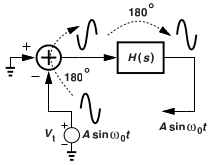
\includegraphics[scale=0.8]{slike/osc_feedback_4.png}
%	 \caption{Пропагација синусоиде кроз петљу на фреквенцији $\omega_{0}$.}
%	 \label{osc_feedback_4}
%\end{figure}
\begin{figure}[!ht]
    \centering
    \vspace{0.5cm}
    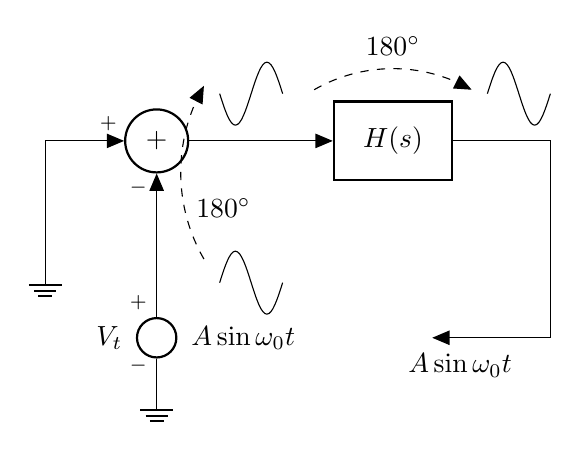
\begin{tikzpicture}[auto, >=triangle 45]
    
    \node [draw, circle, thick, minimum size=0.8cm, inner sep=0] (sum) {$+$};
    \node [draw, circle, thick, minimum size=0.5cm, below of=sum, node distance=2.5cm, inner sep=0] (circvt) {};
    \node [draw, rectangle, thick, minimum width=1.5cm, minimum height=1cm, right of=sum, node distance=3cm] (block) {$H(s)$};
    \node [right of=block, node distance=2cm] (out) {};
    \node [below of=out, node distance=2.5cm] (out1) {};
    \node [left of=out1, node distance=1.5cm] (out2) {};
    \node [draw, ground, below left of=sum, node distance=2cm] (gnd1) {};
    \node [draw, ground, below of=circvt, node distance=0.5cm] (gnd2) {};
    \node [left of=circvt, node distance=0.6cm] {$V_{t}$};
    \node [right of=circvt, node distance=1.1cm] {$A\sin\omega_{0}t$};
    \node [below right of=out2, node distance=0.5cm] {$A\sin\omega_{0}t$};
    \node [below right of=sum, node distance=1.2cm] {$180^{\circ}$};
    \node [above of=block, node distance=1.2cm] {$180^{\circ}$};

    \draw (0.8,0.6) sin (1,0.2) cos (1.2,0.6) sin (1.4,1) cos (1.6,0.6);
    \draw (0.8,-1.8) sin (1,-1.4) cos (1.2,-1.8) sin (1.4,-2.2) cos (1.6,-1.8);
    \draw (4.2,0.6) sin (4.4,1) cos (4.6,0.6) sin (4.8,0.2) cos (5,0.6);

    \draw[->,dashed,rotate=-90] (1.5,0.6) arc[start angle=-60, end angle=-120, radius=2.2];
    \draw[->,dashed, rotate=180] (-2,-0.65) arc[start angle=-60, end angle=-120, radius=2];

    \draw[->] (gnd1) |- node [pos=0.9] {\scriptsize $+$} (sum);
    \draw[-] (gnd2) -- node [pos=0.6] {\scriptsize $-$} (circvt);
    \draw[->] (circvt) -- node [pos=0.1] {\scriptsize $+$} node [pos=0.9] {\scriptsize $-$} (sum);
    \draw[->] (sum) -- (block);
    \draw[-] (block) -- (out.center) -- (out1.center);
    \draw[->] (out1.center) -- (out2.center);
    \end{tikzpicture}
    %\vspace{0.5cm}
    \caption{Пропагација синусоиде кроз петљу на учестаности $\omega_{0}$.}
    \label{osc_feedback_4}
\end{figure}

Укупан фазни помјерај од $360^{\circ}$ на $\omega_{0}$ имплицира да се сигнал враћа да би се појачао док кружи у петљи. Ова појава доводи до пораста амплитуде јер је враћени сигнал бар толико велик као и почетни сигнал, односно зато што је $|H(j\omega_{0})|=1$. Стога се услови за осциловање сумирају као:
\begin{equation} 
	\label{osc_condition_1}
	|H(j\omega_{0})| = 1
\end{equation}
\begin{equation} 
	\label{osc_condition_2}
	\angle H(j\omega_{0}) = -180^{\circ},
\end{equation}
и називају се Баркхаузеновим критеријумима~\cite{Razavi:PLL_CMOS_2020}. Услов $H(j\omega_{0})=-1$ се назива и услов покретања или почетни услов. \par
Нагомилавање осцилација се такође може посматрати и у временском домену. Са Слике~\ref{osc_feedback_5a} се примјећује да је, са $H(j\omega_{0})=-1$, излаз једнак улазу, али помјерен за $180^{\circ}$. Ако је петља затворена (\figurename~\ref{osc_feedback_5b}), излаз се одузима од улаза, што даје већу амплитуду (замах) на $A$. Тај сигнал се затим поново инвертује и одузима од улаза, и тако у круг, што доводи до неограниченог раста амплитуде (\figurename~\ref{osc_feedback_5c}). \par
%\begin{figure}[!ht]
%	 \centering
%	 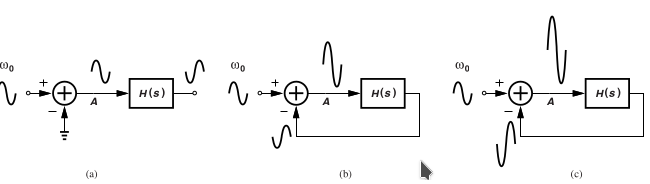
\includegraphics[scale=0.65]{slike/osc_feedback_5.png}
%	 \caption{Раст амплитуде улазне синусоиде кроз петљу у току времена.}
%	 \label{osc_feedback_5}
%\end{figure}
\begin{figure}[!ht]
    \centering
    %\vspace{0.5cm}

    \subfloat[]{
    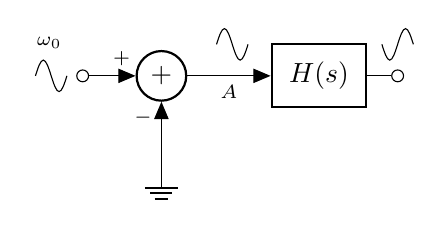
\begin{tikzpicture}[auto, >=triangle 45]
    
    %\node at (0, 0) {};
    \node [draw, circle, thick, minimum size=0.63cm, inner sep=0] (sum) {$+$};
    \node [draw, circle, minimum size=0.15cm, left of=sum, inner sep=0] (circin) {};
    \node [above left of=circin, node distance=0.6cm] (omega) {\scriptsize $\omega_{0}$};
    \node [right of=sum, node distance=2cm] (block) [draw, rectangle, thick, minimum width=1.2cm, minimum height=0.8cm] {$H(s)$};
    \node [draw, circle, minimum size=0.15cm, right of=block, inner sep=0] (circout) {};
    \node [draw, ground, below of=sum, node distance=1cm] (gnd) {};

    \draw (-1.6,0) sin (-1.5,0.2) cos (-1.4,0) sin (-1.3,-0.2) cos (-1.2,0);
    \draw (0.7,0.4) sin (0.8,0.6) cos (0.9,0.4) sin (1.0,0.2) cos (1.1,0.4);
    \draw (2.8,0.4) sin (2.9,0.2) cos (3.0,0.4) sin (3.1,0.6) cos (3.2,0.4);

    \draw[->] (circin) -- node [pos=0.7] {\scriptsize $+$} (sum);
    \draw[->] (gnd) -- node [pos=0.7] {\scriptsize $-$} (sum);
    \draw[->] (sum) -- node [pos=0.5, below of=sum, node distance=0.2cm] {\scriptsize $A$} (block);
    \draw[-] (block) -- (circout);

    \end{tikzpicture}
    \label{osc_feedback_5a}
    }
    \hfil
    \subfloat[]{
    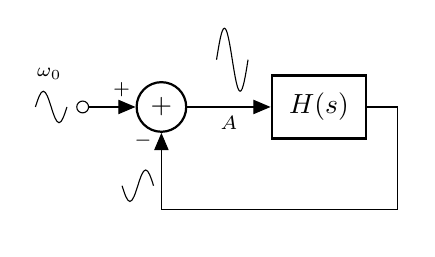
\begin{tikzpicture}[auto, >=triangle 45]
    
    %\node at (0, 0) {};
    \node [draw, circle, thick, minimum size=0.63cm, inner sep=0] (sum) {$+$};
    \node [draw, circle, minimum size=0.15cm, left of=sum, inner sep=0] (circin) {};
    \node [above left of=circin, node distance=0.6cm] (omega) {\scriptsize $\omega_{0}$};
    \node [right of=sum, node distance=2cm] (block) [draw, rectangle, thick, minimum width=1.2cm, minimum height=0.8cm] {$H(s)$};
    \node [right of=block] (out) {};
    %\node [draw, ground, below of=sum1, node distance=1cm] (gnd) {};

    \draw (-1.6,0) sin (-1.5,0.2) cos (-1.4,0) sin (-1.3,-0.2) cos (-1.2,0);
    \draw (0.7,0.6) sin (0.8,1) cos (0.9,0.6) sin (1.0,0.2) cos (1.1,0.6);
    \draw (-0.5,-1) sin (-0.4,-1.2) cos (-0.3,-1) sin (-0.2,-0.8) cos (-0.1,-1);

    \draw[->] (circin) -- node [pos=0.7] {\scriptsize $+$} (sum);
    %\draw[->] (gnd) -- node [pos=0.7] {\scriptsize $-$} (sum1);
    \draw[->] (sum) -- node [pos=0.5, below of=sum, node distance=0.2cm] {\scriptsize $A$} (block);
    \draw[->] (block) -- (out.center) |- ++(0,-1.3) -| node[pos=0.05] {} node[pos=0.95] {\scriptsize $-$} (sum);

    \end{tikzpicture}
    \label{osc_feedback_5b}
    }
    \hfil
    \subfloat[]{
    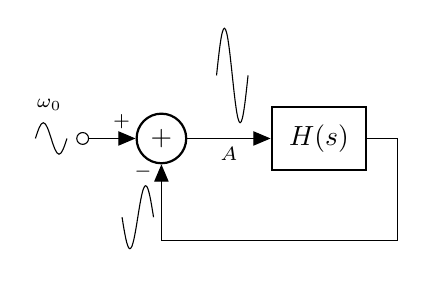
\begin{tikzpicture}[auto, >=triangle 45]
    
    %\node at (0, 0) {};
    \node [draw, circle, thick, minimum size=0.63cm, inner sep=0] (sum) {$+$};
    \node [draw, circle, minimum size=0.15cm, left of=sum, inner sep=0] (circin) {};
    \node [above left of=circin, node distance=0.6cm] (omega) {\scriptsize $\omega_{0}$};
    \node [right of=sum, node distance=2cm] (block) [draw, rectangle, thick, minimum width=1.2cm, minimum height=0.8cm] {$H(s)$};
    \node [right of=block] (out) {};
    %\node [draw, ground, below of=sum1, node distance=1cm] (gnd) {};

    \draw (-1.6,0) sin (-1.5,0.2) cos (-1.4,0) sin (-1.3,-0.2) cos (-1.2,0);
    \draw (0.7,0.8) sin (0.8,1.4) cos (0.9,0.8) sin (1.0,0.2) cos (1.1,0.8);
    \draw (-0.5,-1) sin (-0.4,-1.4) cos (-0.3,-1) sin (-0.2,-0.6) cos (-0.1,-1);

    \draw[->] (circin) -- node [pos=0.7] {\scriptsize $+$} (sum);
    %\draw[->] (gnd) -- node [pos=0.7] {\scriptsize $-$} (sum1);
    \draw[->] (sum) -- node [pos=0.5, below of=sum, node distance=0.2cm] {\scriptsize $A$} (block);
    \draw[->] (block) -- (out.center) |- ++(0,-1.3) -| node[pos=0.05] {} node[pos=0.95] {\scriptsize $-$} (sum);

    \end{tikzpicture}
    \label{osc_feedback_5c}
    }
    %\vspace{0.5cm}
    \caption{Раст амплитуде улазне синусоиде кроз петљу у току времена.}
    \label{osc_feedback_5}
\end{figure}

Укратко, систем са негативном повратном спрегом може да генерише растући периодични излаз као одговор на синусоидни улаз ако његово појачање у петљи достигне -1 на коначној учестаности, $\omega_{0}$. Али, да ли такав систем осцилује ако не примjенимо никакав улаз? Одговор је да, јер широкопојасни шум уређаја унутар петље има коначну енергију у близини $\omega_{0}$, стварајући малу компоненту која кружи у петљи и изазива осцилације. Нпр. као што је приказано на Слици~\ref{osc_feedback_6}, извор шума, $V_{n}$, на улазу $H(s)$ даје излаз који је једнак:
\begin{equation} 
	\label{osc_feedback_eq_8}
	Y = V_{n}\frac{H(s)}{1+H(s)},
\end{equation}
чиме се доводи до неограниченог појачања за $s=j\omega_{0}$. То такође значи да, чак иако је $V_{n}$ бесконачно мало на $\omega_{0}$, на $Y$ се може претпоставити појављивање неке коначне амплитуде осциловања тј. замаха \engl{Swing}.
%\begin{figure}[!ht]
%	 \centering
%	 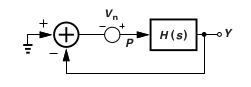
\includegraphics[scale=0.8]{slike/osc_feedback_6.png}
%	 \caption{Утицај шума убризганог у систем затворене петље.}
%	 \label{osc_feedback_6}
%\end{figure}
\begin{figure}[!ht]
    \centering
    \vspace{0.5cm}
    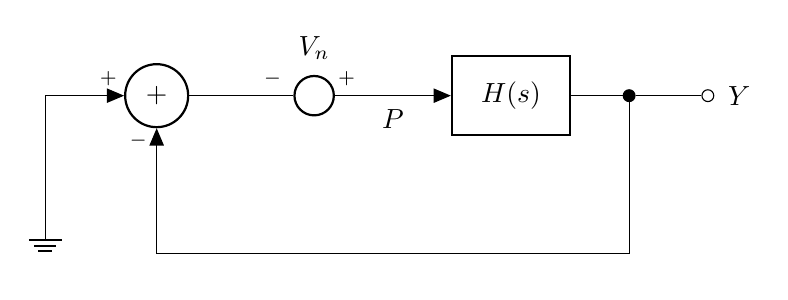
\begin{tikzpicture}[auto, >=triangle 45]
    
    \node [draw, circle, thick, minimum size=0.8cm, inner sep=0] (sum) {$+$};
    \node [draw, circle, thick, minimum size=0.5cm, right of=sum, node distance=2cm, inner sep=0] (circvn) {};
    \node [draw, rectangle, thick, minimum width=1.5cm, minimum height=1cm, right of=circvn, node distance=2.5cm] (block) {$H(s)$};
    \node [draw, circle, minimum size=0.15cm, inner sep=0,  fill=black, right of=block, node distance=1.5cm] (out) {};
    \node [draw, ground, below left of=sum, node distance=2cm] (gnd) {};
    \node [draw, circle, minimum size=0.15cm, right of=out, inner sep=0] (circy) {};
    \node [above of=circvn, node distance=0.6cm] {$V_{n}$};
    \node [right of=circy, node distance=0.4cm] {$Y$};

    \draw[->] (gnd) |- node [pos=0.9] {\scriptsize $+$} (sum);
    \draw[-] (sum) -- node [pos=0.8] {\scriptsize $-$} (circvn);
    \draw[->] (circvn) -- node [pos=0.1] {\scriptsize $+$} node [pos=0.5, below of=circvn, node distance=0.3cm] {$P$} (block);
    \draw[-] (out) -- (circy);
    \draw[->] (block) -- (out) |- ++(0,-2) -| node[pos=0.05] {} node[pos=0.95] {\scriptsize $-$} (sum);

    \end{tikzpicture}
    \caption{Извор шума у систему затворене петље.}
    \label{osc_feedback_6}
\end{figure}


\subsection{Основе прстенастог осцилатора}
Прстенасти осцилатори су у данашње вријеме веома популарни у \PLL\ системима захваљујући својој прилагодљивости дизајна и широког опсега подешавања учестаности. Ово поглавље уопштено разматра основе прстенастих осцилатора, да би се стекло дубље разумијевање рада коришћеног дигитално контролисаног осцилатора, чији конкретан дизајн је описан у поглављу~\ref{DCO chapter}. \par
\figurename~\ref{ring_osc_1} приказује основни концепт прстенастог осцилатора са три степена. Ако се користи само један степен, тада се не обезбјеђује довољан фазни помјерај да би важио услов из једначине~\ref{osc_condition_2}. Чак и примјеном два степена, систем не може да осцилује јер $\angle H(j\omega_{0})$ достиже $-180^{\circ}$ тек за $\omega=\infty$~\cite{Razavi:PLL_CMOS_2020}. Због тога се претпоставља да коришћењем три степена могу бити задовољени услови из једначина~\ref{osc_condition_1} и~\ref{osc_condition_2}, па се стога врши даља анализа како би се то и показало. \par 
На Слици~\ref{ring_osc_1}, коло означено испрекиданом линијом је означено са $-H(s)$ да би било у складу са системом негативне повратне спреге приказаним на Слици~\ref{osc_feedback_2}. \par
%\begin{figure}[!ht]
%	 \centering
%	 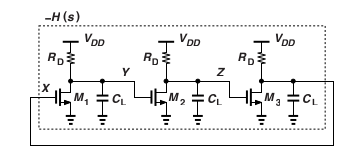
\includegraphics[scale=0.8]{slike/ring_osc_1.png}
%	 \caption{Три степена са заједничким извором у повратној спрези.}
%	 \label{ring_osc_1}
%\end{figure}
\begin{figure}[!ht]
    \centering
    \vspace{0.2cm}

    \begin{tikzpicture}[scale=1]
    \ctikzset{tripoles/mos style/arrows}
    \ctikzset{tripoles/pmos style/emptycircle}
    \ctikzset{logic ports=ieee}

    % Stage 1
    \begin{scope}[shift={(0,0)}, name=stage1]
    \draw 
    (0,0) --++ (0,-0.5) node[nmos, anchor=D] (M1) {$\text{M}_1$} % NMOS transistor
    (M1.S) node[ground] {} % Ground connection
    (M1.D) --++ (0,0.5) to[R, l=$R_D$] (0,2) node[rground, rotate=180] {} ++ (0,0.7) node (anchor=south)(Vdd) {$V_\text{DD}$} % Resistor connected to Vdd
    %(M1.G) -- (-2,0) coordinate (V3) % Feedback loop connection
    (M1.G) --++ (-0.5,0) node[anchor=south west] (X) {$X$}
    (M1.G) --++ (-1,0) node[circle, anchor=center] (G1) {}
    (M1.D) to [short, *-] (1.5, -0.5) node[circ] (V1) {} % Output node
    to[C, l=$C_L$] (V1 |- M1.S) node[ground] {}; % Capacitor connected to ground
    \end{scope}

    % Stage 2
    \begin{scope}[shift={(5,0)}, name=stage2]
    \draw 
    % Stage 1
    (0,0) --++ (0,-0.5) node[nmos, anchor=D] (M2) {$\text{M}_2$} % NMOS transistor
    (M2.S) node[ground] {} % Ground connection
    (M2.D) --++ (0,0.5) to[R, l=$R_D$] (0,2) node[rground, rotate=180] {} ++ (0,0.7) node (anchor=south)(Vdd) {$V_\text{DD}$} % Resistor connected to Vdd
    %(M1.G) -- (-2,0) coordinate (V3) % Feedback loop connection
    (M2.G) --++ (-0.5,0) node[anchor=south west] (Y) {$Y$}
    (M2.G) --++ (-0.7,0) node[circle, anchor=center] (G2) {}
    (M2.D) to [short, *-] (1.5, -0.5) node[circ] (V2) {} % Output node
    to[C, l=$C_L$] (V2 |- M2.S) node[ground] {}; % Capacitor connected to ground
    \end{scope}
    %\draw (2,0) node[nmos, anchor=D] (M2) {} % NMOS transistor
    %(M2.S) -- (2,-2) node[ground] {} % Ground connection
    %(M2.D) to[R, l=$R_2$] (2,2) to[Vdd] {} % Resistor connected to Vdd
    %(M2.G) -- (V1) % Gate connected to output of Stage 1
    %(2,0) -- (4,0) node[circ] (V2) {} % Output node
    %to[C, l=$C_2$] (V2 |- M2.S) node[ground] {}; % Capacitor connected to ground

    % Stage 3
    \begin{scope}[shift={(10,0)}, name=stage3]
    \draw 
    % Stage 1
    (0,0) --++ (0,-0.5) node[nmos, anchor=D] (M3) {$\text{M}_3$} % NMOS transistor
    (M3.S) node[ground] {} % Ground connection
    (M3.D) --++ (0,0.5) to[R, l=$R_D$] (0,2) node[rground, rotate=180] {} ++ (0,0.7) node (anchor=south)(Vdd) {$V_\text{DD}$} % Resistor connected to Vdd
    %(M1.G) -- (-2,0) coordinate (V3) % Feedback loop connection
    (M3.G) --++ (-0.5,0) node[anchor=south west] (Z) {$Z$}
    (M3.G) --++ (-0.7,0) node[circle, anchor=center] (G3) {}
    (M3.D) to [short, *-] (1.5, -0.5) node[circ] (V3) {} % Output node
    to[C, l=$C_L$] (V3 |- M3.S) node[ground] {}; % Capacitor connected to ground
    \end{scope}

    \draw (V1) -| (G2.center);
    \draw (V2) -| (G3.center);
    \draw (V3) --++ (1.8,0) --++ (0,-3.5) -| (G1.center);

    \draw[dashed] (-1.6,0) --++ (0,3.3) node[anchor=south west] (H) {$-H(s)$} --++ (14.5,0) --++ (0,-6.5) --++ (-14.5,0) --++ (0,3.2);
    %\draw[-] (scope2.V1) -| (scope3.Z);
    %\draw (4,0) node[nmos, anchor=D] (M3) {} % NMOS transistor
    %(M3.S) -- (4,-2) node[ground] {} % Ground connection
    %(M3.D) to[R, l=$R_3$] (4,2) to[Vdd] {} % Resistor connected to Vdd
    %(M3.G) -- (V2) % Gate connected to output of Stage 2
    %(4,0) -- (6,0) node[circ] (V3) {} % Output node
    %to[C, l=$C_3$] (V3 |- M3.S) node[ground] {}; % Capacitor connected to ground

    % Feedback loop from Stage 3 to Stage 1
    %\draw (V3) |- (-2,0) -- (M1.G);
    %(0,0)
    %node[nmos, scale=1](nmos1){}
    %(nmos1.D) to [short] ++(0,-0.5) node[R, scale=1](r1){}
    %(nmos1.S) to [short] node[ground](gnd1){}
    %;
    \end{tikzpicture}
    \vspace{0.2cm}
    \caption{Три степена са заједничким извором у повратној спрези.}
    \label{ring_osc_1}
\end{figure}

%\begin{figure}[!ht]
%	 \centering
%	 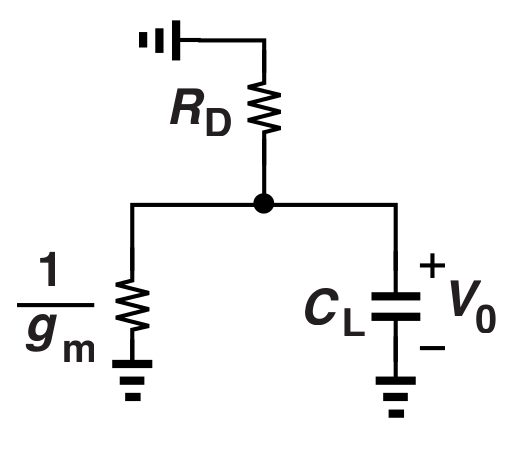
\includegraphics[scale=0.2]{slike/ring_osc_3.png}
%	 \caption{Еквивалентно коло једног степена у петљи.}
%	 \label{ring_osc_2}
%\end{figure}
\begin{figure}[!ht]
    \centering
    \vspace{0.2cm}

    \begin{tikzpicture}[scale=1]
    \ctikzset{tripoles/mos style/arrows}
    \ctikzset{tripoles/pmos style/emptycircle}
    \ctikzset{logic ports=ieee}

    \draw 
    (0,0) --++ (0,0.5) to[R, l=$R_D$] (0,2) |-++ (-1,0.5) node[ground, rotate=-90] {}
    (0,0) -|++ (-2.5,-0.5) to[american controlled current source, name=ccs] (-2.5,-2) |-++ (-1,-1) node[ground] {}
    (-1.9,-1.3) node[anchor=west] {$i_d = g_m v_i$}
    (0,0) -|++ (2.5,-0.5) to[C, l_=$C_L$] (2.5,-2) --++ (0,-1) node[ground] {}
    (0,0) node[circ] {}
    (3.0,-1.25) node[anchor=west] (Vo) {$v_o$}
    (2.7,-0.8) node[anchor=west] {$+$}
    (2.7,-1.7) node[anchor=west] {$-$}

    %(-4.5,-1.25) to[american voltage source, v_=$v_{i}$, name=vs] (-4.5,-3) 
    (-4.5,-1.25) to[american voltages ,V_=$v_i$] (-4.5,-3) 
    (-4.5,-1.25) --++ (1,0) node[draw, circle, minimum size=0.13cm, inner sep=0, fill=white]{}
    (-4.5,-3) --++ (1,0) node[circ]{} --++ (1,0)
    ;

    %$i_{d}=K(V_{I}-V_{T})v_{i}=g_{m}v_{i}$

    \end{tikzpicture}
    \vspace{0.2cm}
    \caption{Еквивалентно коло једног степена у петљи.}
    \label{ring_osc_2}
\end{figure}

На Слици~\ref{ring_osc_2} приказано је еквивалентно коло на нивоу малих сигнала за један степен прстенастог осцилатора приказаног на Слици~\ref{ring_osc_1}. У случају да за тренутак занемаримо капацитивно оптерећење тј. да важи $C_{L}=0$, добија се уобичајена функција одзива појачавача
\begin{equation} 
	\label{osc_feedback_eq_9_0_1}
	v_{o} = -K(V_{I} - V_{T})R_{L}v_{i} = -g_{m}R_{D}v_{i}.
\end{equation}
Када су $v_{i}=V_{i}\cos (\omega t)$ и $C_{L}=0$, тада је напон на излазу једнак
\begin{equation} 
	\label{osc_feedback_eq_9_0_2}
	v_{o} = -g_{m}R_{D}V_{i}\cos (\omega t).
\end{equation}
У једначинама~\ref{osc_feedback_eq_9_0_1} и~\ref{osc_feedback_eq_9_0_2}, са $g_{m}$ је означена транскондуктанса NMOS транзистора која представља фактор појачања транзистора. Она је обрнуто сразмјерна отпорности и уопштено за MOSFET је једнака
\begin{equation} 
	\label{osc_feedback_eq_9_1}
	g_{m} = K(V_{I} - V_{T}),
\end{equation}
гдје је $V_{I}=V_{GS}$ тј. напон од гејта до сорса, $V_{T}$ је напон прага, а $K$ је параметар повезан са физичком структуром MOSFET-a и једнак је
\begin{equation} 
	\label{osc_feedback_eq_9_2}
        K = K_{n} \frac{W}{L}.
\end{equation}
Са $W$ је означена ширина гејта, са $L$ његова дужина, док је $K_{n}$ константа повезана са MOSFET карактеристикама као што је дебљина оксида~\cite{AGARWAL:2005foundations}. \par
Ако се сада и кондензатор узме у разматрање, да би се пронашла веза између $v_i$ и $v_o$ за коло са Слике~\ref{ring_osc_2}, потребно је направити импедансни модел кола, а он је приказан на Слици~\ref{ring_osc_3a}. \par
\begin{figure}[!ht]
    \centering
    \vspace{0.2cm}

    \subfloat[]{
    \begin{tikzpicture}[scale=1]
    \ctikzset{tripoles/mos style/arrows}
    \ctikzset{tripoles/pmos style/emptycircle}
    \ctikzset{logic ports=ieee}

    \draw 
    (0,0) --++ (0,0.5) to[R, l=$R_D$] (0,2) |-++ (-1,0.5) node[ground, rotate=-90] {}
    (0,0) -|++ (-2.5,-0.5) to[american controlled current source, name=ccs] (-2.5,-2) |-++ (-1,-1) node[ground] {}
    (-1.9,-1.3) node[anchor=west] {$I_d = g_m V_i$}
    (0,0) -|++ (2.5,-0.5) to[C, l_=$\dfrac{1}{sC_L}$] (2.5,-2) --++ (0,-1) node[ground] {}
    (0,0) node[circ] {}
    (3.0,-1.25) node[anchor=west] (Vo) {$V_o$}
    (2.7,-0.8) node[anchor=west] {$+$}
    (2.7,-1.7) node[anchor=west] {$-$}

    %(-4.5,-1.25) to[american voltage source, v_=$v_{i}$, name=vs] (-4.5,-3) 
    (-4.5,-1.25) to[american voltages ,V_=$V_i$] (-4.5,-3) 
    (-4.5,-1.25) --++ (1,0) node[draw, circle, minimum size=0.13cm, inner sep=0, fill=white]{}
    (-4.5,-3) --++ (1,0) node[circ]{} --++ (1,0)
    ;

    %$i_{d}=K(V_{I}-V_{T})v_{i}=g_{m}v_{i}$

    \end{tikzpicture}
    \label{ring_osc_3a}
    }
    \vfil
    \vspace{0.3cm}
    \subfloat[]{
    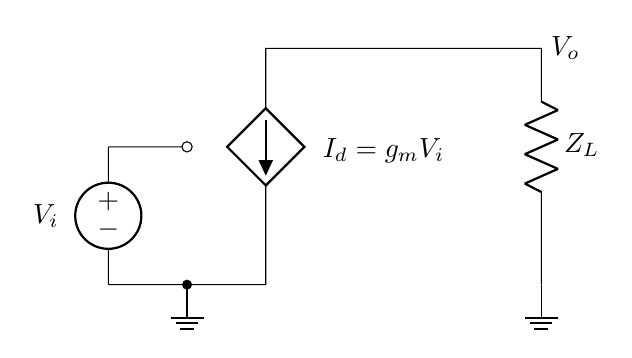
\begin{tikzpicture}[scale=1]
    \ctikzset{tripoles/mos style/arrows}
    \ctikzset{tripoles/pmos style/emptycircle}
    \ctikzset{logic ports=ieee}

    \draw 
    (0,0) -|++ (-2.5,-0.5) to[american controlled current source, name=ccs] (-2.5,-2) |-++ (-1,-1) node[ground] {}
    (-1.9,-1.3) node[anchor=west] {$I_d = g_m V_i$}
    (0,0) -|++ (1,-0.5) to[R, l=$Z_L$] (1,-2) --++ (0,-1) node[ground] {}
    (1,0) node[anchor=west] (Vo) {$V_o$}
    (-4.5,-1.25) to[american voltages ,V_=$V_i$] (-4.5,-3) 
    (-4.5,-1.25) --++ (1,0) node[draw, circle, minimum size=0.13cm, inner sep=0, fill=white]{}
    (-4.5,-3) --++ (1,0) node[circ]{} --++ (1,0)
    ;

    \end{tikzpicture}
    \label{ring_osc_3b}
    }
    \vspace{0.2cm}
    \caption{Импедансни модел еквивалентног кола једног степена у петљи.}
    \label{ring_osc_3}
\end{figure}

Ефективнa вриједност импедансе оптерећења, $Z_L$ (\figurename~\ref{ring_osc_3b}) дата је са
\begin{equation} 
	\label{osc_feedback_eq_9_0_3}
	Z_L = R_{D} || \dfrac{1}{sC_L}.
\end{equation}
Тада је израз за амплитуду излаза ($V_o$) једнак 
\begin{equation} 
	\label{osc_feedback_eq_9_0_4}
	V_o = -g_{m}Z_{L}V_{i} = -g_{m}\left(R_{D}\,||\,\dfrac{1}{sC_{L}}\right)V_{i}.
\end{equation}
То је еквивалентно са
\begin{equation} 
	\label{osc_feedback_eq_9_0_5}
	\frac{V_o}{V_i} = -g_{m}\left(R_{D}\,||\,\dfrac{1}{sC_{L}}\right).
\end{equation}
Како је једначина~\ref{osc_feedback_eq_9_0_5} изведена за један степен, тада за преносну функцију тростепеног прстена са Слике~\ref{ring_osc_1} важи~\cite{Razavi:PLL_CMOS_2020}
\begin{equation} 
	\label{osc_feedback_eq_9}
	-H(s) = \left[-g_{m}\left(R_{D}\,||\,\frac{1}{sC_{L}}\right)\right]^{3}.
\end{equation}
Ако је $s=j\omega_{0}$, тада једначину~\ref{osc_feedback_eq_9} пишемо као
\begin{equation} 
	\label{osc_feedback_eq_10}
	\displaystyle
	H(j\omega_{0}) = \left[g_{m}\left(R_{D}\|\frac{1}{C_{L}j\omega_{0}}\right)\right]^{3} = \left(\frac{g_{m}R_{D}\displaystyle\frac{1}{C_{L}j\omega_{0}}}{R_{D}+\displaystyle\frac{1}{C_{L}j\omega_{0}}}\right)^{3} = \left(\frac{g_{m}R_{D}}{1+R_{D}C_{L}j\omega_{0}}\right)^{3}.
\end{equation}
Добијени резултат представља комплексни разломак који даље желимо представити у стандардном комплексном облику $z = x + jy$:
\begin{equation} 
	\label{osc_feedback_eq_11}
	\displaystyle
	\begin{split}
		H(j\omega_{0}) &= \left(\frac{g_{m}R_{D}}{1+R_{D}C_{L}j\omega_{0}}\cdot\frac{1-R_{D}C_{L}j\omega_{0}}{1-R_{D}C_{L}j\omega_{0}}\right)^{3} = \\
			       &= \left(\frac{g_{m}R_{D}-g_{m}R_{D}^{2}C_{L}j\omega_{0}}{1+R_{D}^{2}C_{L}^{2}\omega_{0}^{2}}\right)^{3} = \\
			       &= \left(\frac{g_{m}R_{D}}{1+R_{D}^{2}C_{L}^{2}\omega_{0}^2}-j\frac{g_{m}R_{D}^{2}C_{L}\omega_{0}}{1+R_{D}^{2}C_{L}^{2}\omega_{0}^{2}}\right)^{3}.
	\end{split}
\end{equation}
Да би се поставио услов $|H(j\omega_{0})|=1$, потребно је наћи модул (интензитет) степеноване вриједности комплексног израза добијеног изнад. Рецимо да имамо неки комплексан број $z=x+jy$. Он се може представити и у поларном облику као
\begin{equation}
	\label{compl_1}
	z = A(\text{cos}\theta + j\text{sin}\theta),
\end{equation}
гдје су:
\begin{itemize}
	\item $A = |z| \rightarrow$ модул (апсолутна вриједност) комплексног броја,
	\item $\theta = \text{arg}(z) = \displaystyle \text{arctan}\left(\frac{y}{x}\right) \rightarrow$ фазни угао (аргумент).
\end{itemize}
Коришћењем Ојлерове формуле, $e^{j\theta} = \text{cos}\theta + j\text{sin}\theta$, комплексни број можемо представити као
\begin{equation}
	\label{compl_2}
	z = Ae^{j\theta}.
\end{equation}
Ако тако представљен комплексни број степенујемо неким природним бројем $n$, добија се
\begin{equation}
	\label{compl_3}
	z^{n} = \left(Ae^{j\theta}\right)^{n} = A^{n}\left(e^{j\theta}\right)^{n} = A^{n}e^{jn\theta}.
\end{equation}
То значи да степеновањем комплексног броја важи следеће:
\begin{enumerate}
	\item Модул комплексног броја се подиже на исти степен.
	\item Фазни угао се множи са вриједношћу степена.
\end{enumerate}
Ако се први закључак примијени на наш случај, важи следеће:
\begin{equation} 
	\label{osc_feedback_eq_12}
	\displaystyle
	\begin{split}
		|H(j\omega_{0})| &= \left|\frac{g_{m}R_{D}}{1+R_{D}^{2}C_{L}^{2}\omega_{0}^2}-j\frac{g_{m}R_{D}^{2}C_{L}\omega_{0}}{1+R_{D}^{2}C_{L}^{2}\omega_{0}^{2}}\right|^{3} = \\
				 &= \left(\sqrt{\frac{g_{m}^{2}R_{D}^{2}}{(1+R_{D}^{2}C_{L}^{2}\omega_{0}^{2})^{2}}+\frac{g_{m}^{2}R_{D}^{4}C_{L}^{2}\omega_{0}^{2}}{(1+R_{D}^{2}C_{L}^{2}\omega_{0}^{2})^{2}}}\right)^{3} = \\
				 &= \left(\sqrt{\frac{g_{m}^{2}R_{D}^{2}(1+R_{D}^{2}C_{L}^{2}\omega_{0}^{2})}{(1+R_{D}^{2}C_{L}^{2}\omega_{0}^{2})^{2}}}\right)^{3} = \\
				 &= \left(\frac{g_{m}R_{D}}{\sqrt{1+R_{D}^{2}C_{L}^{2}\omega_{0}^{2}}}\right)^{3}.
	\end{split}
\end{equation}
На основу претходног израза, услов $|H(j\omega_{0})|=1$ се може представити као
\begin{equation}
	\label{osc_feedback_eq_13}
	\displaystyle
	\left(\frac{g_{m}R_{D}}{\sqrt{1+R_{D}^{2}C_{L}^{2}\omega_{0}^{2}}}\right)^{3} = 1.
\end{equation}
Одатле се може изразити $\omega_{0}$ на следећи начин:
\begin{equation}
	\label{osc_feedback_eq_14}
	\displaystyle
	\omega_{0} = \frac{\sqrt{g_{m}^{2}R_{D}^{2}-1}}{R_{D}C_{L}}.
\end{equation}
Ако сада други закључак примјенимо на фазни угао преносне функције, тада ће $\angle H(j\omega_{0})$ бити једнак
\begin{equation}
	\label{osc_feedback_eq_15}
	\displaystyle
	\begin{split}
		\angle H(j\omega_{0}) &= 3\cdot\text{arctan}\left(\frac{\displaystyle -\frac{g_{m}R_{D}^{2}C_{L}\omega_{0}}{1+R_{D}^{2}C_{L}^{2}\omega_{0}^2}}{\displaystyle \frac{g_{m}R_{D}}{1+R_{D}^{2}C_{L}^{2}\omega_{0}^2}}\right) = \\
				     &= 3\cdot\text{arctan}(-R_{D}C_{L}\omega_{0}) = \\
				     &= -3\cdot\text{arctan}(R_{D}C_{L}\omega_{0}).
	\end{split}
\end{equation}
На основу претходног израза, услов $\angle H(j\omega_{0}) = -180^{\circ}$ може се представити као
\begin{equation}
	\label{osc_feedback_eq_16}
	\displaystyle
	\text{arctan}(R_{D}C_{L}\omega_{0}) = 60^{\circ}.
\end{equation}
Одатле се може представити $\omega_{0}$ на следећи начин:
\begin{equation}
	\label{osc_feedback_eq_17}
	\displaystyle
	\omega_{0} = \frac{\sqrt{3}}{R_{D}C_{L}}.
\end{equation}
Ако сада изједначимо изразе~\ref{osc_feedback_eq_14}~и~\ref{osc_feedback_eq_17}, добија се:
\begin{equation}
	\label{osc_feedback_eq_18}
	\displaystyle
	\frac{\sqrt{g_{m}^{2}R_{D}^{2}-1}}{R_{D}C_{L}} = \frac{\sqrt{3}}{R_{D}C_{L}}.
\end{equation}
Одатле се даље добија:
\begin{equation}
	\label{osc_feedback_eq_19}
	\displaystyle
	g_{m}R_{D} = 2.
\end{equation}
Другим ријечима, сваки степен мора обезбједити појачање напона ниске фреквенције од 2, да бе се гарантовало осциловање~\cite{Razavi:PLL_CMOS_2020}. \par
У општем случају, ако се уведе $N$ идентичних степени у прстен, гдје је $N$ непаран број, петља обезбјеђује негативну повратну спрегу на ниским учестаностима, што захтјева фазни помјерај од $-180^{\circ}/N$ по једном степену да би систем осциловао. Тада ће $\omega_{0}$ бити једнако
\begin{equation}
	\label{osc_feedback_eq_20}
	\displaystyle
	\omega_{0} = \frac{1}{R_{D}C_{L}}\text{tan}\frac{180^{\circ}}{N}.
\end{equation}
Како се $N$ повећава, $\omega_{0}$ опада јер свака фаза мора унијети мање фазног помјераја. Такође, у општем случају, како $N$ расте, захтијевано нискофреквентно појачање се смањује што се може видјети из израза
\begin{equation}
	\label{osc_feedback_eq_21}
	\displaystyle
	g_{m}R_{D} = \sqrt{\text{tan}^{2}\frac{180^{\circ}}{N}+1}.
\end{equation}
Видјели смо да су таласни облици прстенастог осцилаотра блиски синусоиди за $|H(j\omega_{0})|=1$. Meђутим, они почињу да личе на квадратни талас ако је $|H(j\omega_{0})|$ знатно изнад 1. Већина апликација тежи оштријим прелазима сигнала како би се осигурало брзо укључивање и искључивање уређаја. Стога су квадратни таласни облици пожељнији за примјену, и у те сврхе се уводи инверторски прстен обрађен у наредном поглављу.

\subsubsection{Инверторски прстен}
Најчешћа имплементација прстенастих осцилатора је коришћењем CMOS инвертора умјесто отпорнички оптерећених појачавача као фаза појачања у прстену. \figurename~\ref{inv_ring_osc_1} приказује тростепени инверторски прстен. Ако претпоставимо да је у почетку $V_{X} = V_{Y} = V_{Z}$, свака фаза уводи напонско појачање од $-(g_{mN}+g_{mP})(r_{ON}||r_{OP})$, које типично има вриједност преко 2~\cite{Razavi:PLL_CMOS_2020}. Након тога, шум унутар компоненти узрокује обнављање сигнала све док амплитуда осциловања не достигне пун напонски опсег \engl{Rail-to-Rail}. \par
%\begin{figure}[!ht]
%	 \centering
%	 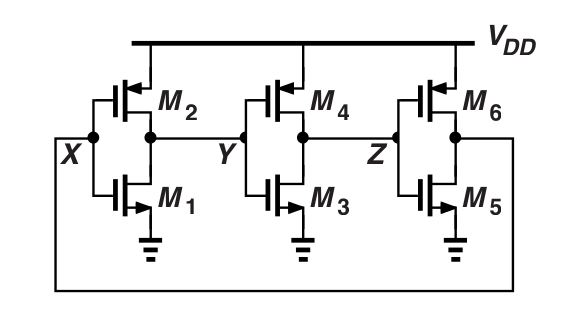
\includegraphics[scale=0.4]{slike/inv_ring_osc_1.png}
%	 \caption{Тростепени прстенасти осцилатор састављен од CMOS инвертора.}
%	 \label{inv_ring_osc_1}
%\end{figure}
\begin{figure}[!ht]
    \centering
    \vspace{0.2cm}
    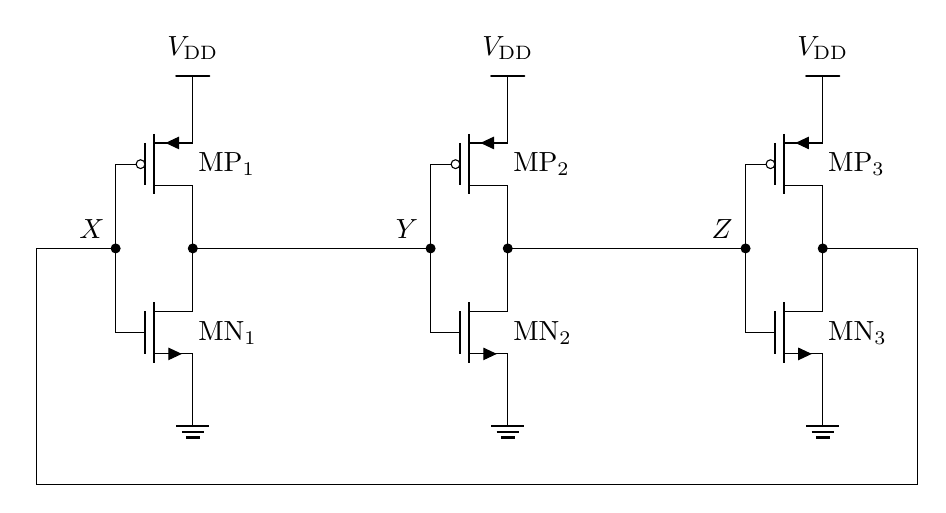
\begin{tikzpicture}[scale=1]
        \ctikzset{tripoles/mos style/arrows}
        \ctikzset{tripoles/pmos style/emptycircle}
        \ctikzset{logic ports=ieee}
        
	\begin{scope}[shift={(0,0)}]
	\draw 
	(0,0) --++ (0,0.3) node[pmos, anchor=D](p1){$\text{MP}_1$}
        (0,0) --++ (0,-0.3) node[nmos, anchor=D](n1){$\text{MN}_1$}
	(p1.S) node[rground, rotate=180] {} ++ (0,0.7) node (anchor=south)(Vdd) {$V_\text{DD}$}
	(n1.S) node[ground] {}
        (p1.G) to (n1.G)
	($(p1.G)!0.5!(n1.G)$) node[circ] () {} --++ (-1,0) node[] (in1) {} ++ (0.7,0) node[anchor=south] {$X$}
	($(p1.D)!0.5!(n1.D)$) node[circ] (out1) {}
	;
        \end{scope}
	
	\begin{scope}[shift={(4,0)}]
	\draw 
        (0,0) --++ (0,0.3) node[pmos, anchor=D](p2){$\text{MP}_2$}
        (0,0) --++ (0,-0.3) node[nmos, anchor=D](n2){$\text{MN}_2$}
	(p2.S) node[rground, rotate=180] {} ++ (0,0.7) node (anchor=south)(Vdd) {$V_\text{DD}$}
	(n2.S) node[ground] {}
        (p2.G) to (n2.G)
	($(p2.G)!0.5!(n2.G)$) node[circ] () {} --++ (-1,0) node[] (in2) {} ++ (0.7,0) node[anchor=south] {$Y$}
	($(p2.D)!0.5!(n2.D)$) node[circ] (out2) {}
	;
        \end{scope}
        

	\begin{scope}[shift={(8,0)}]
	\draw 
        (0,0) --++ (0,0.3) node[pmos, anchor=D](p3){$\text{MP}_3$}
        (0,0) --++ (0,-0.3) node[nmos, anchor=D](n3){$\text{MN}_3$}
	(p3.S) node[rground, rotate=180] {} ++ (0,0.7) node (anchor=south)(Vdd) {$V_\text{DD}$}
	(n3.S) node[ground] {}
        (p3.G) to (n3.G)
	($(p3.G)!0.5!(n3.G)$) node[circ] () {} --++ (-1,0) node[] (in3) {} ++ (0.7,0) node[anchor=south] {$Z$}
	($(p3.D)!0.5!(n3.D)$) node[circ] (out3) {}
	;
        \end{scope}


	\draw (out1) -- (in2.center);
	\draw (out2) -- (in3.center);
	\draw (out3) --++ (1.2,0) --++ (0,-3) -| (in1.center);

    \end{tikzpicture}
    \vspace{0.2cm}
    \caption{Тростепени прстенасти осцилатор састављен од CMOS инвертора.}
    \label{inv_ring_osc_1}
\end{figure}

Шта ако, након укључења, прстен почиње са једним чвором на нули? Рецимо, ако је $V_{X}=0$, тада је $V_{Y}=V_\text{DD}$, а $V_{Z}=0$, што значи да трећи инвертор подиже $V_{X}$ на $V_\text{DD}$. \figurename~\ref{inv_ring_osc_2} приказује идеализоване облике сигнала на сва три степена у прстену, у току времена. Закључујемо да прелаз на једном чвору узрокује прелаз на наредном након одређеног кашњења, $T_{D}$. Укупан период осциловања је стога једнак $6T_{D}$, па је учестаност осциловања једнака $f=1/6T_{D}$.\par
%\begin{figure}[!ht]
%	 \centering
%	 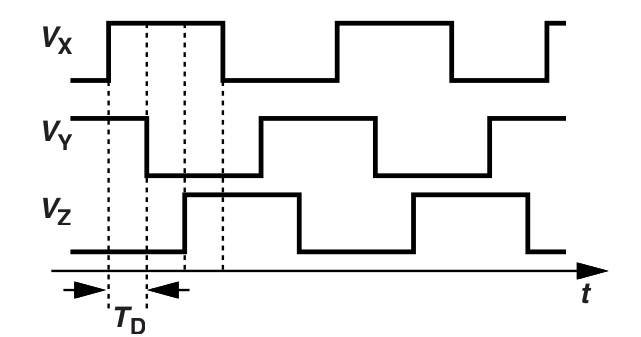
\includegraphics[scale=0.4]{slike/inv_ring_osc_2.png}
%	 \caption{Облици сигнала на чворовима.}
%	 \label{inv_ring_osc_2}
%\end{figure}
\begin{figure}[!ht]
    \centering
    \vspace{0.5cm}
    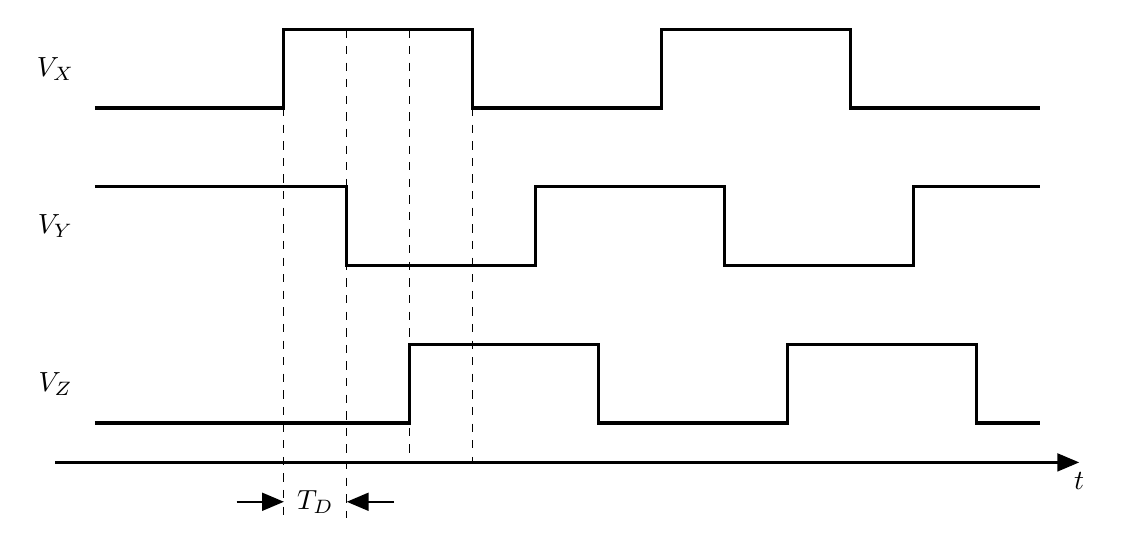
\begin{tikzpicture}[>=triangle 45]

	\def \lx {0}
	\def \hx {1}
	\def \ly {-2}
	\def \hy {-1}
	\def \lz {-4}
	\def \hz {-3}

        % Vx
        \draw[very thick] (0,\lx) -- (2.4,\lx) -- (2.4,\hx) -- (4.8,\hx) -- (4.8,\lx) -- (7.2,\lx) -- (7.2,\hx) -- (9.6,\hx) -- (9.6,\lx) -- (12,\lx);
	\node at (-0.5,0.5) {$V_X$};
        
	% Vy
        \draw[very thick] (0,\hy) -- (3.2,\hy) -- (3.2,\ly) -- (5.6,\ly) -- (5.6,\hy) -- (8,\hy) -- (8,\ly) -- (10.4,\ly) -- (10.4,\hy) -- (12,\hy);
	\node at (-0.5,-1.5) {$V_Y$};
        
	% Vz
        \draw[very thick] (0,\lz) -- (4,\lz) -- (4,\hz) -- (6.4,\hz) -- (6.4,\lz) -- (8.8,\lz) -- (8.8,\hz) -- (11.2,\hz) -- (11.2,\lz) -- (12,\lz);
	\node at (-0.5,-3.5) {$V_Z$};

	\draw[->, thick] (-0.5,-4.5) -- (12.5,-4.5) node[anchor=north] {$t$};

	\node at (2.8,-5) {$T_D$}; 

	\draw[dashed] (2.4,\lx) -- (2.4,-5.2);
	\draw[dashed] (3.2,\hx) -- (3.2,-5.2);
	\draw[dashed] (4.0,\hx) -- (4.0,-4.5);
	\draw[dashed] (4.8,\lx) -- (4.8,-4.5);

	\draw[->, thick] (1.8,-5) -- (2.4,-5);
	\draw[->, thick] (3.8,-5) -- (3.2,-5);
    
    \end{tikzpicture}
    \vspace{0.5cm}
    \caption{Облици дигиталног сигнала на фазама инверторског прстена.}
    \label{inv_ring_osc_2}
\end{figure}

Стварни облици сигнала претходног осцилатора нису тако оштри као на Слици~\ref{inv_ring_osc_2}, али нису ни правилни као синусоида. Реалнији примјер је илустрован на Слици~\ref{inv_ring_osc_3a}, гдје $V_{X}$ мијења правац чим достигне $V_\text{DD}$ или 0, због кратког кашњења кроз петљу. Поређења ради, петостепени прстен омогућава осцилације са периодом $10T_{D}$, дозвољавајући сигналу на $V_{X}$ да дуже времена остане на високом, односно ниском напонском нивоу (\figurename~\ref{inv_ring_osc_3b}). \par
%\begin{figure}[!ht]
%	 \centering
%	 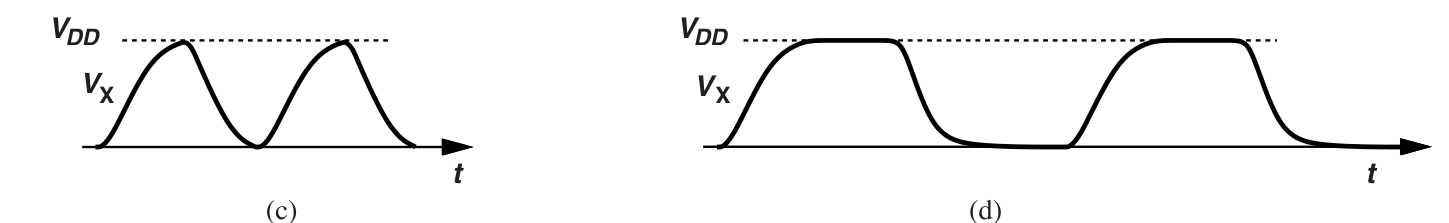
\includegraphics[scale=0.3]{slike/inv_ring_osc_3.png}
%	 \caption{Реалан облик сигнала (а) тростепеног и (б) петостепеног прстенастог осцилатора.}
%	 \label{inv_ring_osc_3}
%\end{figure}
\begin{figure}[!ht]
    \centering
    %\vspace{0.5cm}

    \subfloat[]{
    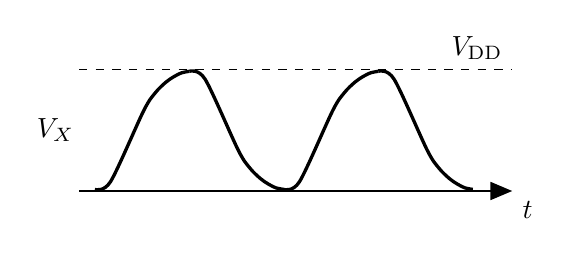
\begin{tikzpicture}[>=triangle 45]
    
    % Axis and labels
    \draw[->, thick] (0,-0.02) -- (5.5,-0.02) node[below right] {$t$};
    \draw[dashed] (0,1.52) -- (5.5,1.52) node[above left] {$V_\text{DD}$};
    \node at (-0.3,0.75) {$V_X$};

    % Period 1
    \begin{scope}[shift={(0.2,0)}]
    % Posedge
    \draw[very thick] plot[smooth] coordinates {
    (0,0) (0.2,0.1) (0.62,1) (0.77,1.23) (0.9,1.36) (1,1.43) (1.1, 1.48) (1.2,1.5)};
    % Negedge
    \draw[very thick] plot[smooth] coordinates {
    (1.2,1.5) (1.4,1.4) (1.82,0.5) (1.97,0.27) (2.1,0.14) (2.2,0.07) (2.3,0.02) (2.4,0.0)};
    \end{scope}

    % Period 2
    \begin{scope}[shift={(2.6,0)}]
    % Posedge
    \draw[very thick] plot[smooth] coordinates {
    (0,0) (0.2,0.1) (0.62,1) (0.77,1.23) (0.9,1.36) (1,1.43) (1.1, 1.48) (1.2,1.5)};
    % Negedge
    \draw[very thick] plot[smooth] coordinates {
    (1.2,1.5) (1.4,1.4) (1.82,0.5) (1.97,0.27) (2.1,0.14) (2.2,0.07) (2.3,0.02) (2.4,0.0)};
    \end{scope}

    \end{tikzpicture}
    \label{inv_ring_osc_3a}
    }

    \subfloat[]{
    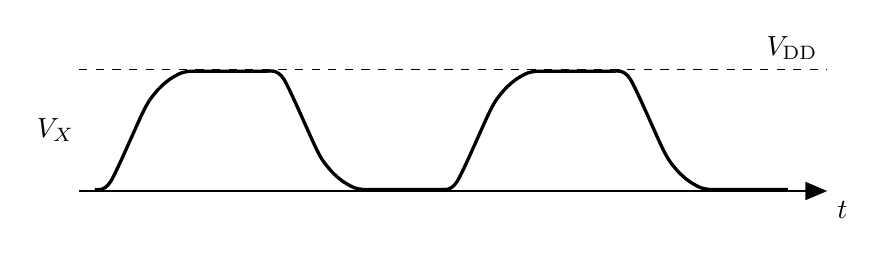
\begin{tikzpicture}[>=triangle 45]

    % Axis and labels
    \draw[->, thick] (0,-0.02) -- (9.5,-0.02) node[below right] {$t$};
    \draw[dashed] (0,1.52) -- (9.5,1.52) node[above left] {$V_\text{DD}$};
    \node at (-0.3,0.75) {$V_X$};

    % Period 1
    \begin{scope}[shift={(0.2,0)}]
    % Posedge
    \draw[very thick] plot[smooth] coordinates {
    (0,0) (0.2,0.1) (0.62,1) (0.77,1.23) (0.9,1.36) (1,1.43) (1.1, 1.48) (1.2,1.5) (1.3,1.5) (2.2,1.5)};
    % Negedge
    \draw[very thick] plot[smooth] coordinates {
    (2.2,1.5) (2.4,1.4) (2.82,0.5) (2.97,0.27) (3.1,0.14) (3.2,0.07) (3.3,0.02) (3.4,0) (3.5,0) (4.5,0)};
    \end{scope}

    % Period 2
    \begin{scope}[shift={(4.6,0)}]
    % Posedge
    \draw[very thick] plot[smooth] coordinates {
    (0,0) (0.2,0.1) (0.62,1) (0.77,1.23) (0.9,1.36) (1,1.43) (1.1, 1.48) (1.2,1.5) (1.3,1.5) (2.2,1.5)};
    % Negedge
    \draw[very thick] plot[smooth] coordinates {
    (2.2,1.5) (2.4,1.4) (2.82,0.5) (2.97,0.27) (3.1,0.14) (3.2,0.07) (3.3,0.02) (3.4,0) (3.5,0) (4.4,0)};
    \end{scope}
    
    \end{tikzpicture}
    \label{inv_ring_osc_3b}
    }
    %\vspace{0.5cm}
    \caption{Реалан облик сигнала (а) тростепеног и (б) петостепеног прстенастог осцилатора.}
    \label{inv_ring_osc_3}
\end{figure}

Прстенасти осцилатори су уопштено прилично осјетљиви на вриједности напона напајања. Прво, максимална учестаност осциловања расте како расте напон напајања. Друго, динамичка потрошња снаге прстенастог осцилатора има чак квадратну зависност од вриједности напона напајања, о чему ће више ријечи бити у поглављу~\ref{DCO chapter}.

\subsection{Шум у осцилаторима} \label{section:osc:noise}
За идеалан осцилатор који ради на учестаности $\omega_{c}$, сва његова снага је концентрисана на једну учестаност, $\omega_{c}$, као што је приказано на Слици~\ref{fig:osc:noise_1a}. У реалном осцилатору, спектар се шири на околне учестаности око $\omega_{c}$ (\figurename~\ref{fig:osc:noise_1b}). У осцилаторима се такво ширење назива фазни шум. \par
%\begin{figure}[!ht]
%	 \centering
%	 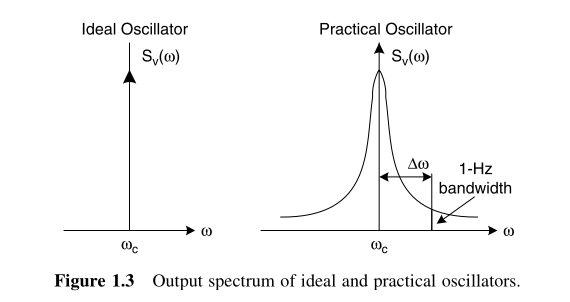
\includegraphics[scale=0.6]{slike/osc_noise_1.png}
%	 \caption{Излазни спектар (а) идеалног и (б) реалног осцилатора.}
%	 \label{fig:osc:noise_1}
%\end{figure}
\begin{figure}[!ht]
    \centering
    %\vspace{0.5cm}

    \subfloat[]{
    \begin{tikzpicture}[>=triangle 45, scale=1.5]
    
    % Ideal Oscillator
    \draw[->, thick] (0,0) -- (2.4,0) node[right] {$\omega$};
    \draw[->, thick] (1.2,0) -- (1.2,3) node[above] {$S_v(\omega)$};
    %\draw[thick] (1,0) -- (1,1.8);
    \node at (1.2,-0.3) {$\omega_c$};
    \node at (1.2,3.7) {Идеални осцилатор};

    \end{tikzpicture}
    \label{fig:osc:noise_1a}
    }
    \hspace{1.5cm}
    \subfloat[]{
    \begin{tikzpicture}[>=triangle 45, scale=1.5]
    
    % Practical Oscillator
    \draw[->, thick] (0,0) -- (4,0) node[right] {$\omega$};
    \draw[->, thick] (2,0) -- (2,3) node[above] {$S_v(\omega)$};
    
    % Drawing the curve
    \draw[thick] plot[domain=0.5:3.5, samples=100] (\x, {0.2 + 2.5*exp(-4*(\x-2)^2)});
    
    % Vertical line at wc
    % \draw[dashed, thick] (2,0) -- (2,2);

    \draw[-] (2.8,0) -- (2.8,0.8); 
    \draw[-] (2.85,0) -- (2.85,0.8); 

    % Delta omega and bandwidth labels
    \draw[<->] (2,0.7) -- node[midway, below] {$\Delta \omega$} (2.8,0.7);
    \draw[->] (3.4,0.6) -- node[near start, above, anchor=south west] {Опсег од 1\,Hz} (2.87,0.1);

    % Omega_c label
    \node at (2,-0.3) {$\omega_c$};
    \node at (2,3.7) {Реални осцилатор};
    
    \end{tikzpicture}
    \label{fig:osc:noise_1b}
    }
    %\vspace{0.5cm}
    \caption{Излазни спектар (а) идеалног и (б) реалног осцилатора.}
    \label{fig:osc:noise_1}
\end{figure}

Фазни шум се обично карактерише у фреквенцијском домену. За идеалан осцилатор који ради на учестаности $\omega_{c}$, излазни напон може бити изражен као
\begin{equation}
	\label{eq:osc:noise:vt_1}
	v(t) = A\cos(\omega_{c}t + \phi),
\end{equation}
гдје је $A$ амплитуда, а $\phi$ је произвољна, али фиксна референтна фаза. Снага је концентрисана на једну учестаност $\omega_{c}$. Еквивалентно, спектар снаге се може записати као
\begin{equation}
	\label{eq:osc:noise:sv_1}
	S_{v}(\omega) = \frac{A^{2}}{2}\delta (\omega - \omega_{c}),
\end{equation}
гдје је $\delta$ јединични имплус или Диракова делта функција (\figurename~\ref{fig:osc:noise_1a}). Међутим, у реалном осцилатору и амплитуда и фаза су временски промјенљиве, и спектар ће се зато ширити око учестаности носиоца на околне учестаности. У већини случајева, поремећај у амплитуди је занемарљив или неважан, а и може се лако уклонити додавањем кола која ограничавају амплитуду~\cite{Staszewski:FREQUENCY_SYNTHESIZER_CMOS_2005}. Стога се разматра само насумично одступање фазе:
\begin{equation}
	\label{eq:osc:noise:vt_2}
	v(t) = A\cos[\omega_{c}t + \phi (t)],
\end{equation}
гдје је $\phi (t)$ мало насумично одступање фазе које представља варијације у периоду и најчешће се назива фазни шум. За мале вриједности варијација фазног шума, $|\phi (t)| \ll 1\,\text{rad}$, једначина~\ref{eq:osc:noise:vt_2} се може поједноставити на
\begin{equation}
	\label{eq:osc:noise:vt_3}
	v(t) = A\cos\omega_{c}t + A\phi (t)\sin\omega_{c}(t),
\end{equation}
што значи да се спектар $\phi (t)$ фреквенцијски преводи у $\pm \omega_{c}$. \par
Фазни шум се може квантификовати узимањем опсега од 1\,Hz на растојању $\Delta\omega$ од носиоца, затим рачунањем снаге шума у том опсегу и дијељењем тог резултата са снагом носиоца~\cite{Staszewski:FREQUENCY_SYNTHESIZER_CMOS_2005}. То се назива једнострани \engl{single-sided} фазни шум и изражава се у јединици децибела по херцу [dBc/Hz]. По конвенцији, „c“ у „dBc“ значи „у односу на носилац“.
\begin{equation}
	\label{eq:osc:noise:L_1}
	\mathcal{L} (\Delta\omega) = 10\log_{10} \left(\frac{\text{снага шума у опсегу од 1\,Hz при учестаности } w_{c}+\Delta\omega}{\text{снага носиоца}}\right)
\end{equation}
Једнострани фазни шум из једначине~\ref{eq:osc:noise:L_1} је половина спектра фазног шума, тј. може се записати као
\begin{equation}
	\label{eq:osc:noise:L_2}
	\mathcal{L} (\Delta\omega) = 10\log_{10} \left(\frac{S_{\phi}(\Delta\omega)}{\text{2}}\right),
\end{equation}
гдје је $S_{\phi}(\Delta\omega)$ дато са
\begin{equation}
	\label{eq:osc:noise:S_phi_1}
	S_{\phi}(\Delta\omega) = \frac{S_{v}(\Delta\omega)}{\text{снага носиоца}}.
\end{equation}
Типични спектар фазног шума осцилатора приказан је на Слици~\ref{fig:osc:noise_2}. У овом логаритамском дијаграму, фазни шум нормализован на dBc/Hz, приказан је у односу на офсет учестаност $\Delta\omega$ од носиоца $\omega_{c}$. \par 
%\begin{figure}[!ht]
%	 \centering
%	 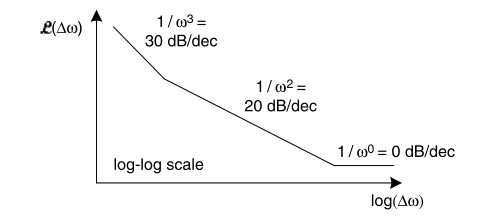
\includegraphics[scale=0.7]{slike/osc_noise_2.png}
%	 \caption{Спектар фазног шума реалног осцилатора.}
%	 \label{fig:osc:noise_2}
%\end{figure}
\begin{figure}[!ht]
    \centering
    \vspace{0.3cm}
    \begin{tikzpicture}[>=triangle 45]
    
    \draw[->, thick] (0,0) -- (11,0) node[right] {$\log (\Delta \omega)$};
    \draw[->, thick] (0,0) -- (0,6) node[above] {$\mathcal{L}(\Delta \omega)$};
    \draw[-, thick] (0.5,5.6) -- (2.5, 3.5) -- (8,0.5) -- (10,0.5);

    \node[anchor=south west] at (1.5, 4.5) {$\dfrac{1}{\omega^3}=30\,\text{dBc/dec}$};
    \node[anchor=south] at (6.1,2.5) {$\dfrac{1}{\omega^2}=20\,\text{dBc/dec}$};
    \node[anchor=south west] at (8, 0.6) {$\dfrac{1}{\omega^0}=0\,\text{dBc/dec}$};
    
    \node[anchor=south west] at (0.3, 0.3) {log-log дијаграм};
    
    \end{tikzpicture}
    %\vspace{0.5cm}
    \caption{Спектар фазног шума реалног осцилатора.}
    \label{fig:osc:noise_2}
\end{figure}

Профил фазног шума прати криву приказану на слици, гдје пролази кроз области са нагибима од $1/\omega^{3}$, $1/\omega^{2}$ и $1/\omega^{0}$. Област $1/\omega^{2}$ се уопштено назива област топлотног шума \engl{Thermal Noise Region} зато што је изазвана тзв. бијелим или неповезаним временским флуктуацијама унутар периода осциловања. Шум треперења \engl{Flicker Noise} $1/f$ електронских уређаја је такође значајан за ниже офсетне учестаности. Он се конвертује навише у $1/\omega^{3}$ област. Коначно, $1/\omega^{0}$ је топлотни електронски шум који се додаје изван осцилатора, као нпр. у излазном баферу, и не утиче на временски одзив осцилатора. 

\section{Дигитално контролисани осцилатор} \label{DCO chapter}
Дигитално контролисани осцилатор описан у овом раду је прстенасти осцилатор, погодан за систем генерисања такта. Прстенасти осцилатор је каскадна комбинација фаза кашњења повезаних у ланац затворене петље~\cite{Madhusudhana:283751064}. Прстенасте архитектуре су компактније од LC осцилатора и имају доста предности захваљујући својој правилној и периодичној просторној структури. Уопштена структура \DCO-а коришћеног унутар описаног \FLL-а заснована је на матрици тростатичких CMOS инвертора~\cite{Terosiet:340277809}. Ова матрица је састављена од $N$-фазних прстена тростатичких инвертора повезаних паралелно. $N$ представља број \DCO\ фаза (степени) и мора бити непаран број већи или једнак 3.~\figurename~\ref{fig:dco:general} приказује примјер $N$-степеног дигитално контролисаног осцилатора који има један прстен стално укључених инвертора (најдоњи прстен без стрелице управљачког сигнала са доње стране инвертора). \par
%\begin{figure}[!ht]
%	 \centering
%	 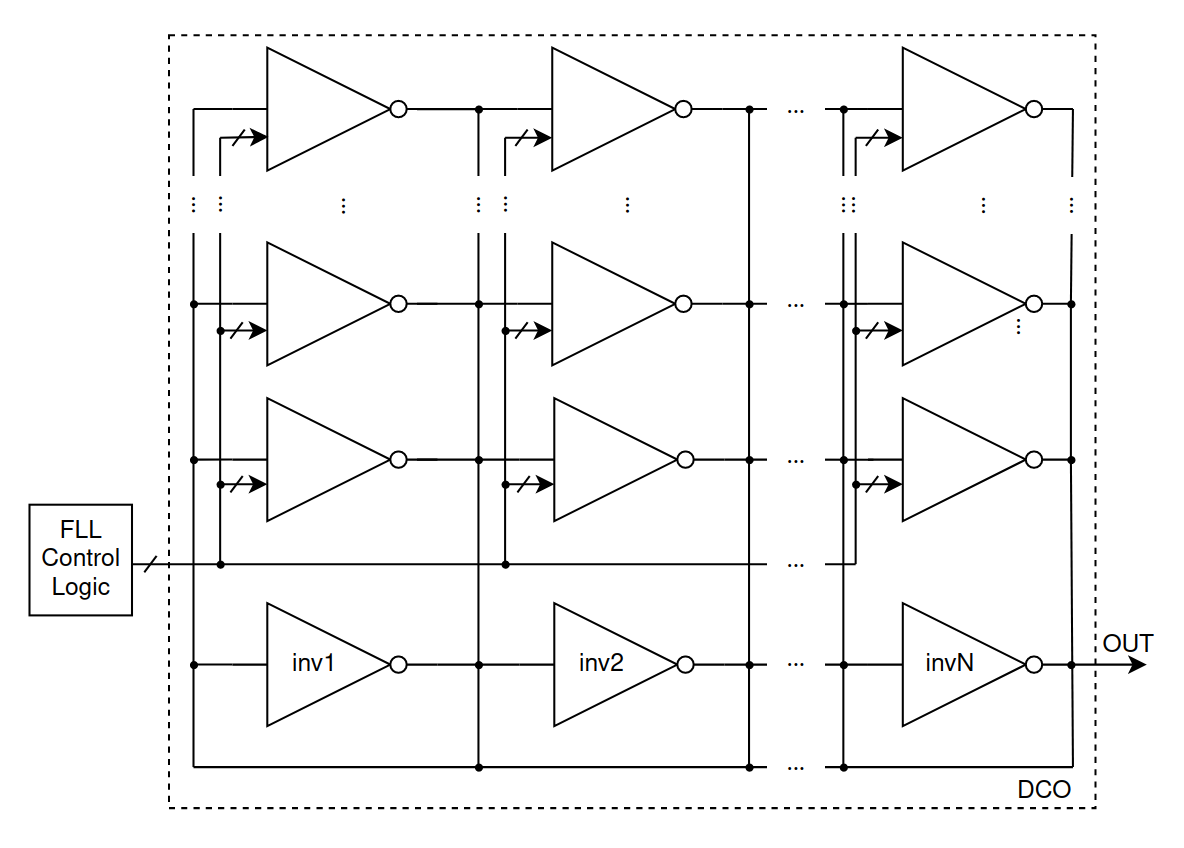
\includegraphics[scale=0.25]{slike/dco_1.png}
%	 \caption{$N$-степени дигитално контролисано осцилатор.}
%	 \label{dco_1}
%\end{figure}
\pgfooclass{InvRow}{
    \method InvRow(){}
    \method apply(#1,#2,#3){
        \draw 
	(#1,#2) node[ieeestd not port, anchor=in, label={[xshift=-0.1cm, yshift=-0.83cm]1}]({#3}0){}
        ({#3}0.out) node[ieeestd not port, anchor=in, label={[xshift=-0.1cm, yshift=-0.83cm]2}]({#3}1){}
	({#3}1.out) --++ (0.7,0) node[anchor=west]{...} ++ (0.65,0) --++ (0.7,0) node[ieeestd not port, anchor=in, label={[xshift=-0.1cm, yshift=-0.83cm]$N$}]({#3}2){};
    }
}
\begin{figure*}[!ht]
\centering
\vspace{0.2cm}
\begin{tikzpicture}[>=triangle 45]
    \ctikzset{tripoles/mos style/arrows}
    \ctikzset{tripoles/pmos style/emptycircle}
    \ctikzset{logic ports=ieee}

    \pgfoonew \invRow=new InvRow()

    \invRow.apply(0,0,i0)
    \invRow.apply(0,1.75,i1)
    \invRow.apply(0,3.5,i2)
    %
    \foreach \x in {0,1,2}
    \draw[] ({i0}\x.out) -- ({i1}\x.out) -- ({i2}\x.out) --++ (0,0.8) node[anchor=west, rotate=90](lcont\x){...};
    \draw[] ({i0}2.in) -- ({i1}2.in) -- ({i2}2.in) --++ (0,0.8) node[anchor=west, rotate=90](lcont6){...};
    \draw ({i0}0.in) -- ({i1}0.in) -- ({i2}0.in) --++ (0,0.8) node[anchor=west, rotate=90](lcont5){...};
    %
    \invRow.apply(0,5.8,i3)
    %
    \foreach \x in {0,1,2}
        \draw (lcont\x.east) -- ({i3}\x.out);
    \draw (lcont5.east) -- ({i3}0.in);
    \draw (lcont6.east) -- ({i3}2.in);
    %
    % BOTTOM ARROWS FOR ALL INVERTERS
    \foreach \r in {1,2,3}{
        \foreach \c in {0,1,2}{
	    \draw[->] ({i\r}\c.down) ++ (0,-0.5) -- ({i\r}\c.down);
        };
    };

    % Circles at inputs and outputs
    \node[circ] at ({i0}0.out){};
    \node[circ] at ({i0}1.out){};
    \node[circ] at ({i0}2.in){};
    \node[circ] at ({i0}2.out){};
    
    \node[circ] at ({i1}0.in){};
    \node[circ] at ({i1}0.out){};
    \node[circ] at ({i1}1.out){};
    \node[circ] at ({i1}2.in){};
    \node[circ] at ({i1}2.out){};

    \node[circ] at ({i2}0.in){};
    \node[circ] at ({i2}0.out){};
    \node[circ] at ({i2}1.out){};
    \node[circ] at ({i2}2.in){};
    \node[circ] at ({i2}2.out){};

    \node[circ] at ({i3}0.in){};
    \node[circ] at ({i3}0.out){};
    \node[circ] at ({i3}1.out){};
    \node[circ] at ({i3}2.in){};
    \node[circ] at ({i3}2.out){};

    %\draw ({i3}0.in) --++ (0,1) --++ (4.05,0) node[anchor=west]{...} ++ (0.65,0) -| ({i3}2.out);
    \draw ({i3}0.in) --++ (0,1) -| ({i3}2.out);

    \draw ({i0}0.out) --++ (0,-1) node[draw, circle, minimum size=0.13cm, inner sep=0, fill=white](ph0){};
    \draw (ph0) ++ (0,-0.1) node[anchor=north]{\scriptsize Фаза 1};

    \draw ({i0}1.out) --++ (0,-1) node[draw, circle, minimum size=0.13cm, inner sep=0, fill=white](ph1){};
    \draw (ph1) ++ (0,-0.1) node[anchor=north]{\scriptsize Фаза 2};
    
    \draw ({i0}2.in) --++ (0,-1) node[draw, circle, minimum size=0.13cm, inner sep=0, fill=white](phNminus1){};
    \draw (phNminus1) ++ (0,-0.1) node[anchor=north]{\scriptsize Фаза $N$-1};
    
    \draw ({i0}2.out) --++ (0,-1) node[draw, circle, minimum size=0.13cm, inner sep=0, fill=white](phN){};
    \draw (phN) ++ (0,-0.1) node[anchor=north]{\scriptsize Фаза $N$};

\end{tikzpicture}
\caption{$N$-степени дигитално контролисани осцилатор.}
\label{fig:dco:general}
\end{figure*}

%(за осцилатор са једним излазним сигналом у односу на заједничко уземљење)
У физичком смислу, матрица може бити преобликована у квадрат, што омогућава једноставнију управљачку логику. На Слици~\ref{fig:dco:general}, основну учестаност \DCO-а дефинише само један прстен који је стално укључен, а у општем случају их може бити више. Остали тростатички инвертори се укључују и искључују у зависности од управљачке логике. \par
Формула за учестаност осциловања \DCO-a гласи:
\begin{equation} \label{f_osc}
    f_\text{osc} = \dfrac{1}{2Nt_\text{d}} \approx \dfrac{I_\text{d}}{2NC_\text{load}V_\text{DDL}},
\end{equation} \\
гдје је $N$ број тростатичких инвертора унутар прстена, $t_\text{d}$ представља кашњење једне ћелије \DCO-a, у чијем саставу је тростатички инвертор (у наставку ће бити детаљније објашњена структура саме ћелије \DCO-а), $I_\text{d}$ је струја која протиче кроз инвертор, $C_\text{load}$ је капацитивно оптерећење истог инвертора, и $V_\text{DDL}$ је напон напајања \DCO-а. Производ $Nt_\text{d}$ је помножен са $2$ да би се добила читава периода такта, а не полупериода. \par
Када је ријеч о топологији, са повећањем броја \DCO\ фаза (степени), фреквенцијски корак ($K_\text{DCO}$) опада, чиме се повећава прецизност \DCO-а. Максимална учестаност осцилатора се се такође смањује, и да би се то надомјестило, напон напајања се може повећати, што с друге стране доводи до веће потрошње снаге. Ако претпоставимо да напон напајања и капацитивно оптерећење по једној фази остану непромјењени, повећање броја фаза не утиче на потрошњу снаге. Међутим, ако укупан број тростатичких инвертора остане непромјењен и подијели се на већи број фаза, то ће довести до смањења капацитивног оптерећења по фазама појединачно, што даље доводи до смањења потрошње снаге. Математичком анализом се то може објаснити на следећи начин: $N$-фазни прстенасти осцилатор који ради на учестаности $f_\text{osc}$ има динамичку потрошњу снаге која се може представити једначином
\begin{equation} 
	\label{eq:dco:dynamic_pwr_1}
    	P = N f_\text{osc} C_\text{tot} V^{2}_\text{DDL}, 
\end{equation}
гдје $C_\text{tot}$ представља укупно капацитивно оптерећење на једној фази. Пошто је учестаност осциловања једнака $f_\text{osc} = 1/(2Nt_\text{d})$, једначину за динамичку снагу можемо написати на следећи начин:
\begin{equation}
    	P = \frac{C_\text{tot}V^{2}_\text{DDL}}{2t_\text{d}},
\end{equation}
одакле се види да је добијена динамичка снага независна од $N$~\cite{Razavi:PLL_CMOS_2020}. \par
С обзиром да је одређени број тростатичких инвертора увијек укључен, \DCO\ има одређену почетну учестаност која не зависи од управљачке ријечи \DCO-а. Тренутна излазна учестаност ће стога у основи зависити од почетне учестаности, фреквенцијског корака тј. резолуције и управљачке ријечи. Стога се може написати следећа линеарна зависност учестаности осциловања, која може послужити за софтверску имплементацију рада \DCO-а~\text{\cite{Milovanovic:8190103}}:  
\begin{equation} \label{f_dco}
	f_\text{DCO} = f_\text{0} + K_\text{DCO} \cdot d,
\end{equation} 
гдје је $f_\text{0}$ почетна учестаност, $K_\text{DCO}$ резолуција учестаности, а $d$ је управљачка дигитална ријеч.

\subsection{Архитектура предложеног \DCO-a}
У овом раду описана је топологија \DCO-a са пет фаза, због тога што је таквом топологијом остварен задовољавајући компромис између учинка и потрошње снаге тј. под задовољавајућим условима се достиже жељена учестаност са довољном прецизношћу. \figurename~\ref{DCO5} приказује структуру \DCO-а коришћеног у описаној \FLL\ имплементацији. \par
\pgfooclass{InvRow}{
    \method InvRow(){}
    \method apply(#1,#2,#3){
        \draw 
        (#1,#2) node[ieeestd not port, anchor=in, scale=0.4, fill=ColorPhase0, fill opacity=\InvFillOpacity]({#3}0){}
        ({#3}0.out) node[ieeestd not port, anchor=in, scale=0.4, fill=ColorPhase1, fill opacity=\InvFillOpacity]({#3}1){}
        ({#3}1.out) node[ieeestd not port, anchor=in, scale=0.4, fill=ColorPhase2, fill opacity=\InvFillOpacity]({#3}2){}
        ({#3}2.out) node[ieeestd not port, anchor=in, scale=0.4, fill=ColorPhase3, fill opacity=\InvFillOpacity]({#3}3){}
        ({#3}3.out) node[ieeestd not port, anchor=in, scale=0.4, fill=ColorPhase4, fill opacity=\InvFillOpacity]({#3}4){};
    }
}
\begin{figure*}[!ht]
\centering
\begin{tikzpicture}[scale=0.95]
    \ctikzset{tripoles/mos style/arrows}
    \ctikzset{tripoles/pmos style/emptycircle}
    \ctikzset{logic ports=ieee}

    \definecolor{ColorPhase0}{RGB}{255,0,0}
    \definecolor{ColorPhase1}{RGB}{192,0,64}
    \definecolor{ColorPhase2}{RGB}{128,0,128}
    \definecolor{ColorPhase3}{RGB}{64,0,192}
    \definecolor{ColorPhase4}{RGB}{0,0,255}

    \definecolor{HLLSColor}{RGB}{64,0,77}
    \definecolor{LHLSColor}{RGB}{106,0,128}

    \definecolor{AlwaysOnBoxColor}{RGB}{0,255,0}
    
    % Color opacity variables
    \def \InvFillOpacity      {1}
    \def \DCOFillOpacity      {0.05}
    \def \CtrlDecFillOpacity  {0.1}
    \def \AlwaysOnBoxOpacity  {0.1}
    \def \HLLSFillOpacity     {0.1}
    \def \HLLSTextOpacity     {1}
    \def \LHLSFillOpacity     {0.05}
    \def \LHLSTextOpacity     {1}
    %
    \pgfoonew \invRow=new InvRow()
    %
    % LEFT INVERTER MATRIX
    \invRow.apply(0,0,i0)
    \invRow.apply(0,0.8,i1)
    \invRow.apply(0,1.6,i2)
    %
    \foreach \x in {0,1,2,3,4}
        \draw ({i0}\x.out) -- ({i1}\x.out) -- ({i2}\x.out) --++ (0,0.5) node[anchor=west, rotate=90, scale=0.5](lcont\x){...};
    \draw ({i0}0.in) -- ({i1}0.in) -- ({i2}0.in) --++ (0,0.5) node[anchor=west, rotate=90, scale=0.5](lcont5){...};
    %
    \invRow.apply(0,3,i3)
    \invRow.apply(0,3.8,i4)
    \invRow.apply(0,4.6,i5)
    %
    \foreach \x in {0,1,2,3,4}
        \draw (lcont\x.east) -- ({i3}\x.out) -- ({i4}\x.out) -- ({i5}\x.out);
    \draw (lcont5.east) -- ({i3}0.in) -- ({i4}0.in) -- ({i5}0.in);
    %
    % RIGHT INVERTER MATRIX
    \invRow.apply(5.8,0,ii0)
    \invRow.apply(5.8,0.8,ii1)
    \invRow.apply(5.8,1.6,ii2)
    %
    \foreach \x in {0,1,2,3,4}
        \draw ({ii0}\x.out) -- ({ii1}\x.out) -- ({ii2}\x.out) --++ (0,0.5) node[anchor=west, rotate=90, scale=0.5](rcont\x){...};
    \draw ({ii0}0.in) -- ({ii1}0.in) -- ({ii2}0.in) --++ (0,0.5) node[anchor=west, rotate=90, scale=0.5](rcont5){...};
    %
    \invRow.apply(5.8,3,ii3)
    \invRow.apply(5.8,3.8,ii4)
    \invRow.apply(5.8,4.6,ii5)
    %
    \foreach \x in {0,1,2,3,4}
        \draw (rcont\x.east) -- ({ii3}\x.out) -- ({ii4}\x.out) -- ({ii5}\x.out);
    \draw (rcont5.east) -- ({ii3}0.in) -- ({ii4}0.in) -- ({ii5}0.in);
    %
    % RECTANGLE FOR ALWAYS ON INVERTERS
    \draw 
    ({i0}0.in) ++ (-0.2,-0.4) node[](ron1){}
    ({i0}0.in) ++ (-0.2,0.4) node[](ron2){}
    ({ii0}4.out) ++ (0.2,0.4) node[](ron3){}
    ({ii0}4.out) ++ (0.2,-0.4) node[](ron4){};
    \filldraw[draw, AlwaysOnBoxColor, fill=AlwaysOnBoxColor, fill opacity=\AlwaysOnBoxOpacity] (ron1.center) -- (ron2.center) -- (ron3.center) -- (ron4.center) -- (ron1.center);
    %
    % UPPER PHASE CONNECTIONS
    \draw ({i5}4.out) ++ (0,1.1) |-++ (0,0.2) node[circ, scale=0.4](circ1){} --++ (0.5,0) node[anchor=west, scale=0.5](contp0){...}
    (contp0.east) -| ({ii5}4.out);
    \draw [dashed] ({i5}4.out) --++ (0,1.1);
    \draw [dashed] ({ii5}0.in) --++ (0,1.1);
    \draw ({ii5}0.in) ++ (0,1.1) --++ (0,0.2) node[circ, scale=0.4](circ2){}
    ({i5}0.in) |- (circ1);
    \foreach \x/\y in {0/1, 1/2, 2/3, 3/4} {
        \draw 
        (contp\x.west) ++ (0,-0.2) node[anchor=west, scale=0.5](contp\y){...}
        ({i5}\x.out) |- (contp\y.west)
        (contp\y.east) -| ({ii5}\x.out);
    }
    \draw
    ({i4}4.out) ++ (0.5,0) node[anchor=west, scale=0.5](contc0){...}
    ({i1}4.out) ++ (0.5,0) node[anchor=west, scale=0.5](contc1){...};
    %
    % BOTTOM ARROWS FOR ALL INVERTERS
    \foreach \r in {0,1,2,3,4,5}{
        \foreach \c in {0,1,2,3,4}{
            \draw ({i\r}\c.down) node[inputarrow, rotate=90, scale = 0.8]{} --++ (0,-0.3);
            \draw ({ii\r}\c.down) node[inputarrow, rotate=90, scale = 0.8]{} --++ (0,-0.3);
        };
    };
    %
    % DCO RECTANGLE
    \draw
    ({i0}0.in) ++ (-0.5,-1.2) node[](r1){}
    ({i5}0.in) ++ (-0.5,1.6) node[](r2){}
    ({ii5}4.out) ++ (0.5,1.6) node[](r3){}
    ({ii0}4.out) ++ (0.5,-1.2) node[](r4){}
    (r1) node[anchor=south west](){DCO};
    \filldraw[draw, \DCOColor, fill=\DCOColor, fill opacity=\DCOFillOpacity] (r1.center) -- (r2.center) -- (r3.center) -- (r4.center) -- (r1.center);
    %
    % COLUMN CONTROL RECTANGLE
    \draw
    (r2) ++ (0.5,1.8) node[](rc1){} 
    (r3) ++ (-0.5,1.8) node[](rc4){}
    (rc1) ++ (0,0.5) node[](rc2){}
    (rc4) ++ (0,0.5) node[](rc3){}
    ($(rc1)!0.5!(rc4)$) node[anchor=south, scale=0.8, text=\CtrlDecColor]{Управљање колонама};
    \filldraw[draw, \CtrlDecColor, fill=\CtrlDecColor, fill opacity=\CtrlDecFillOpacity] (rc1.center) -- (rc2.center) -- (rc3.center) -- (rc4.center) -- (rc1.center);
    %
    % HLLS FROM COLUMN CONTROL RECTANGLE
    \foreach \i/\x in {0/0.4, 1/1.15, 2/1.9, 3/2.65, 4/3.4, 5/6.2, 6/6.95, 7/7.7, 8/8.45, 9/9.2} {
        \draw
        (rc1) ++ (\x,0) --++ (0,-0.4) node[inputarrow, rotate=-90](){} node[rectangle, minimum size=3, thick, rotate=-90, anchor=west, scale=0.7, color=HLLSColor, fill=HLLSColor, fill opacity=\HLLSFillOpacity, text opacity=\HLLSTextOpacity, draw](hl\i){HLLS}
        (hl\i.east) --++ (0,-0.4) node[inputarrow, rotate=-90](){};
    }
    \draw
    (hl4.north) ++ (0.67,0) node[anchor=west, scale=0.5](){...}
    %
    % ROW CONTROL RECTANGLE
    (r1) ++ (-1.8,1.6) node[](rr1){} 
    (r2) ++ (-1.8,-1.2) node[](rr4){}
    (rr1) ++ (-0.5,0) node[](rr2){}
    (rr4) ++ (-0.5,0) node[](rr3){}
    ($(rr1)!0.5!(rr4)$) ++ (-0.5,0) node[anchor=north, scale=0.8, rotate=90, text=\CtrlDecColor]{Управљање врстама};
    \filldraw[draw, \CtrlDecColor, fill=\CtrlDecColor, fill opacity=\CtrlDecFillOpacity] (rr1.center) -- (rr2.center) -- (rr3.center) -- (rr4.center) -- (rr1.center);
    %
    % HLLS FROM ROW CONTROL RECTANGLE
    \foreach \i/\y in {0/0.4, 1/1.2, 2/2.5, 3/3.3, 4/4.1} {
        \draw
        (rr1) ++ (0,\y) --++ (0.4,0) node[inputarrow](){} node[rectangle, minimum size=3, thick, anchor=west, scale=0.7, color=HLLSColor, fill=HLLSColor, fill opacity=\HLLSFillOpacity, text opacity=\HLLSTextOpacity, draw](hlr\i){HLLS}
        (hlr\i.east) --++ (0.4,0) node[inputarrow](){};
    }
    \draw 
    (hlr1.north) ++ (0,0.3) node[anchor=west, rotate=90, scale=0.5](){...}
    %
    % LHLS AND PHASE PORTS
    ($(r3)!0.5!(r4)$) node[](rph2){}
    (rph2) ++ (0,0.7) node[](rph1){}
    (rph1) ++ (0,0.7) node[](rph0){}
    (rph2) ++ (0,-0.7) node[](rph3){}
    (rph3) ++ (0,-0.7) node[](rph4){};
    %
    \foreach \i in {0,1,2,3,4} {
        \draw
        (rph\i.center) --++ (0.4,0) node[inputarrow](){} node[rectangle, minimum size=3, thick, anchor=west, scale=0.7, color=LHLSColor, fill=LHLSColor, fill opacity=\LHLSFillOpacity, text opacity=\LHLSTextOpacity, draw](lh\i){LHLS} 
        (lh\i.east) --++ (0.4,0) node[signal, anchor=west, fill=ColorPhase\i, draw](ph\i){} node[inputarrow](){}
        (ph\i.east) node[anchor=west, scale=0.8]{Фаза \i};
    }
\end{tikzpicture}
\caption{Петостепени прстенасти дигитално контролисани осцилатор (\DCO) састављен од тростатичких инвертора, са додатим претварачима напонских нивоа (\HLLS\ и \LHLS) и уоквиреном врстом стално укључених тростатичких инвертора.}
\label{DCO5}
\end{figure*}

Свака фаза \DCO-а састоји се од 54 тростатичка инвертора, што ако помножимо са бројем фаза даје укупно 270 инвертора. Тростатички инвертори су распоређени у 18 редова и 15 колона. Управљачка логика \FLL-a управља са 17 редова и свих 15 колона, што значи да постоји 255 корака учестаности. Преостали ред са 3$\times$5 тростатичких инвертора је стално укључен и на њега не утиче управљачка логика \FLL-а. Што се више тростатичких инвертора у свакој фази укључи под утицајем управљачке логике \FLL-а, повећавају се струја и тренутна снага покретања \engl{Driving Strength} једне фазе, док њено капацитивно оптерећење у суштини остаје константно, што резултује повећањем излазне учестаности осциловања~\cite{Tierno:4443210}. Поред самих тростатичких инвертора, на Слици~\ref{DCO5} се могу уочити и блокови претварача напонког нивоа на управљачким улазима и фазама \DCO-a, чија је намјена детаљно објашњена у поглављу~\ref{LS chapter}.

\subsection{Блок дијаграм ћелије \DCO-a}
Да би се ефикасно подесила излазна учестаност \DCO-а, уведен је скуп управљачких улаза \DCO-а, а то су сигнали \textit{Row On}, \textit{Row Select} и \textit{Column Select}, поменути такође у поглављу~\ref{section:control_decoder}. Према томе, сваки тростатички инвертор садржи сопствену управљачку јединицу у облику И-ИЛИ стандардне ћелије, и заједно граде већи блок назван ћелија \DCO-а. \figurename~\ref{DCO_cell} приказује шему ћелије \DCO-а на нивоу логичких кола и на нивоу CMOS транзистора. Уочава се да И-ИЛИ коло и тростатички инвертор имају заједнички инвертор како би се уштедило на броју транзистора. \par
\begin{figure}[!ht]
    \centering
    \vspace{0.7cm}
    \subfloat[]{
    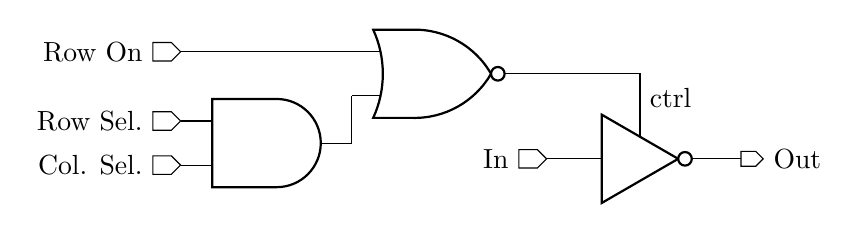
\begin{tikzpicture}[scale=1]
        \ctikzset{tripoles/mos style/arrows}
        \ctikzset{tripoles/pmos style/emptycircle}
        \ctikzset{logic ports=ieee}
        \draw (0,0)
        node[ieeestd not port, anchor=out, scale=1](tsinv){}
        (tsinv.in) --++ (-0.3,0) node[signal, anchor=east, scale=1, draw](pinphi){} 
        (pinphi.west) node[anchor=east, scale=1]{In}
        (tsinv.out) --++ (0.4,0) node[signal, anchor=west, scale=0.8, draw](pinpho){} 
        (pinpho.east) node[anchor=west, scale=1]{Out}
        (tsinv.up) --++ (0,0.5) node[anchor=west, scale=1]{ctrl} |-++ (-1.5,0.3) node[ieeestd nor port, anchor=out, scale=1](nor){}
        (nor.in 2) -|++ (0, -0.6) node[ieeestd and port, anchor=out, scale=1](and){}
        (nor.in 1) -- (and.in 1|-nor.in 1) node[signal, anchor=east, scale=1, draw](pinro){} 
        (pinro.west) node[anchor=east, scale=1]{Row On}       
        (and.in 1) node[signal, anchor=east, scale=1, draw](pinrs){} 
        (pinrs.west) node[anchor=east, scale=1]{Row Sel.}
        (and.in 2) node[signal, anchor=east, scale=1, draw](pincs){} 
        (pincs.west) node[anchor=east, scale=1]{Col. Sel.}
        ;
    \end{tikzpicture}
    \label{DCO_cell_logic_gate_level}
    }
    \hfil
    \vspace{1cm}
    \subfloat[]{
    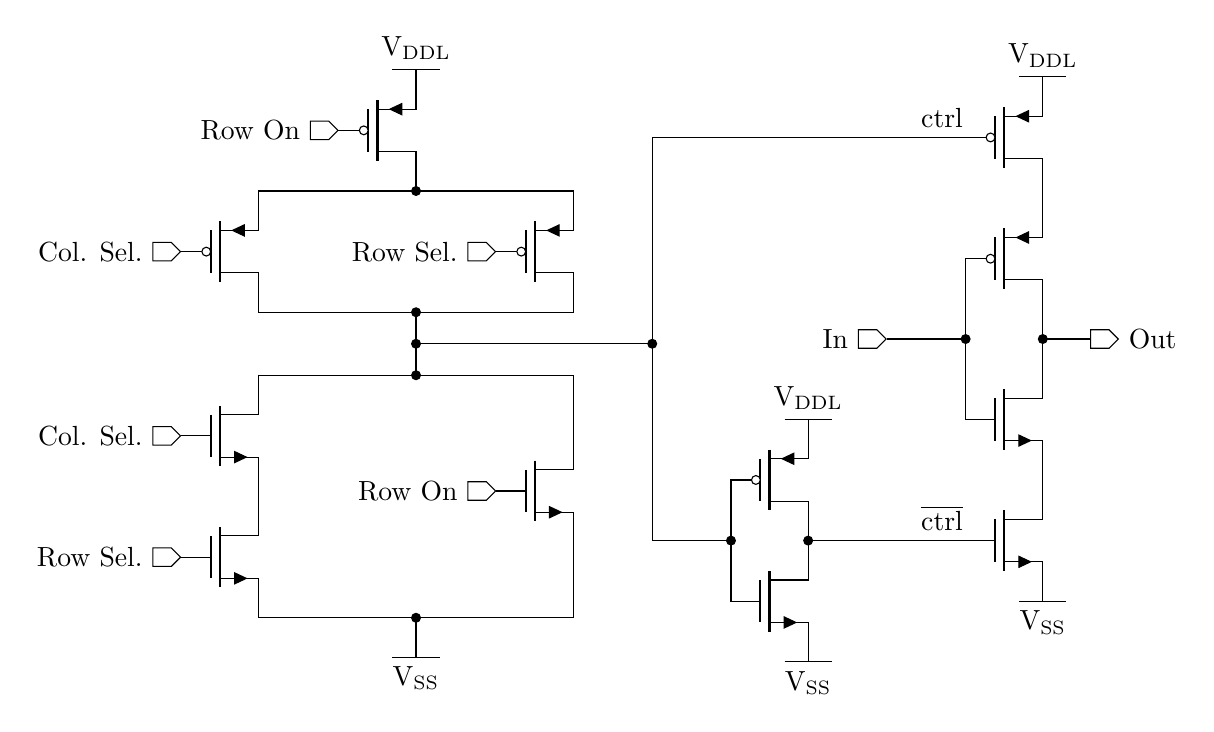
\begin{tikzpicture}[scale=1]
        \ctikzset{tripoles/mos style/arrows}
        \ctikzset{tripoles/pmos style/emptycircle}
        \ctikzset{logic ports=ieee}
        \draw (0,0)
        node[pmos, scale=1](pmos1){}
        (pmos1.D) to [short] ++(0,-0.5) node[nmos, scale=1, anchor=D](nmos1){}
        (pmos1.G) to (nmos1.G)
        ($(pmos1.G)!0.5!(nmos1.G)$) node[circ, scale=1]{} --++ (-1,0) node[signal, anchor=east, scale=1, draw](pinphi){} 
        (pinphi.west) node[anchor=east, scale=1]{In}
        ($(pmos1.D)!0.5!(nmos1.D)$) node[circ, scale=1]{} --++ (0.6,0) node[signal, anchor=west, scale=1, draw](pinpho){} 
        (pinpho.east) node[anchor=west, scale=1]{Out}
        (pmos1.S) node[pmos, scale=1, anchor=D](pmos2){}
        (pmos2.G) ++(-0.3,0) node[anchor=south, scale=1]{ctrl}
        (nmos1.S) node[nmos, scale=1, anchor=D](nmos2){}
        (nmos2.G) --++ (-1,0) |-++ (-1,0) node[circ, scale=1](nctrl){}
        (nmos2.G) ++ (-0.3,0) node[anchor=south, scale=1]{$\overline{\mbox{ctrl}}$}
        (nctrl) node[pmos, scale=1, anchor=D](pinv){}
        (nctrl) node[nmos, scale=1, anchor=D](ninv){}
        (pinv.G) to (ninv.G)
        ($(pinv.G)!0.5!(ninv.G)$) node[circ, scale=1]{} --++ (-1,0) --++ (0,2.5) node[circ, scale=1](pctrl){} |- (pmos2.G)
        (pctrl) --++ (-3,0) node[circ, scale=1](ctrl){}
        (ctrl) --++ (0,0.4) node[circ, scale=1](pside){}
        (ctrl) --++ (0,-0.4) node[circ, scale=1](nside){}
        (pside) ++ (2,0) node[pmos, scale=1, anchor=D](prs){}
        (pside) ++ (-2,0) node[pmos, scale=1, anchor=D](pcs){}
        (prs.G) node[signal, anchor=east, scale=1, draw](pinrs){} 
        (pinrs.west) node[anchor=east, scale=1]{Row Sel.}
        (pcs.G) node[signal, anchor=east, scale=1, draw](pincs){} 
        (pincs.west) node[anchor=east, scale=1]{Col. Sel.}
        (prs.D) to (pcs.D)
        (prs.S) to (pcs.S)
        ($(pcs.S)!0.5!(prs.S)$) node[circ, scale=1]{} node[pmos, scale=1, anchor=D](pro){}
        (pro.G) node[signal, anchor=east, scale=1, draw](pinro){} 
        (pinro.west) node[anchor=east, scale=1]{Row On}
        %
        (nside) ++ (-2,0) node[nmos, scale=1, anchor=D](ncs){}
        (nside) -|++ (2,-0.7) node[nmos, scale=1, anchor=D](nro){}
        (ncs.G) node[signal, anchor=east, scale=1, draw](pinncs){} 
        (pinncs.west) node[anchor=east, scale=1]{Col. Sel.}
        (nro.G) node[signal, anchor=east, scale=1, draw](pinnro){} 
        (pinnro.west) node[anchor=east, scale=1]{Row On}
        (ncs.D) to (nside)
        (ncs.S) node[nmos, scale=1, anchor=D](nrs){}
        (nrs.G) node[signal, anchor=east, scale=1, draw](pinnrs){} 
        (pinnrs.west) node[anchor=east, scale=1]{Row Sel.}
        (nrs.S) --++ (2,0) node[circ, scale=1](vss){} -| (nro.S)
        %
        (vss) --++ (0, -0.5) node[](vss1){} ++ (-0.3,0) --++ (0.6,0) 
	(vss1) node[anchor=north, scale=1]{$\text{V}_\text{SS}$}
        (ninv.S) ++ (-0.3,0) --++ (0.6,0)
	(ninv.S) node[anchor=north, scale=1]{$\text{V}_\text{SS}$}
        (nmos2.S) ++ (-0.3,0) --++ (0.6,0)
	(nmos2.S) node[anchor=north, scale=1]{$\text{V}_\text{SS}$}
        (pmos2.S) ++ (-0.3,0) --++ (0.6,0)
	(pmos2.S) node[anchor=south, scale=1]{$\text{V}_\text{DDL}$}
        (pro.S) ++ (-0.3,0) --++ (0.6,0)
	(pro.S) node[anchor=south, scale=1]{$\text{V}_\text{DDL}$}
        (pinv.S) ++ (-0.3,0) --++ (0.6,0)
	(pinv.S) node[anchor=south, scale=1]{$\text{V}_\text{DDL}$}
        ;
    \end{tikzpicture}
    \label{DCO_cell_transistor_level}
    }
    \caption{Ћелија \DCO-а на нивоу (a) логичких кола и (б) CMOS транзистора.}
    \label{DCO_cell}
\end{figure}

У дигиталном домену сигнал Out може имати три стања. Једно је недефинисано, када је тростатички инвертор искључен. А друга два су када је тростатички инвертор укључен и представљају инвертован сигнал In. Укључивање и искључивање тростатичког инвертора контролише ctrl сигнал који представља излаз из контролног дијела \DCO\ ћелије тј. И-ИЛИ блока стандардне ћелије. За вриједност ctrl сигнала 1, тростатички инвертор је укључен, а за вриједност 0 је искључен. \tablename~\ref{ctrl_truth_table} је таблица истинитости управљачког сигнала ctrl. Логички израз за сигнал ctrl у зависности од управљачких сигнала редова и колона гласи:
\begin{equation}
	\label{dco_cell_ctrl_eq}
	% \text{ctrl} = \overline{(\text{Row Sel.} \cdot \text{Col. Sel.}) + \text{Row On}}
	\text{ctrl} = (\text{Row Sel.} \cdot \text{Col. Sel.}) + \text{Row On}
\end{equation}
\tablename~\ref{out_truth_table} приказује табелу истинитости Out сигнала у зависности од управљачког сигнала ctrl и улазног In. \par
\vspace{0.5cm}
\begin{table}[!ht]
	\caption{Таблица истинитости контролног сигнала тростатичког инвертора.}
	\label{ctrl_truth_table}
	\centering
	\begin{tabular}{|c|c|c||c|}
		\hline
		Row On & Row Sel. & Col. Sel. & ctrl \\
		\specialrule{1pt}{0pt}{0pt}
		0 & 0 & 0 & 0 \\
		\hline
		0 & 0 & 1 & 0 \\
		\hline
		0 & 1 & 0 & 0 \\
		\hline
		0 & 1 & 1 & 1 \\
		\hline
		1 & 0 & 0 & 1 \\
		\hline
		1 & 0 & 1 & 1 \\
		\hline
		1 & 1 & 0 & 1 \\
		\hline
		1 & 1 & 1 & 1 \\
		\hline
	\end{tabular}
\end{table}
\begin{table}[!ht]
	\caption{Таблица истинитости излазног сигнала тростатичког инвертора.}
	\label{out_truth_table}
	\centering
	\begin{tabular}{|c|c||c|}
		\hline
		ctrl & In & Out \\
		\specialrule{1pt}{0pt}{0pt}
		0 & 0 & X \\
		\hline
		0 & 1 & X \\
		\hline
		1 & 0 & 1 \\
		\hline
		1 & 1 & 0 \\
		\hline
	\end{tabular}
\end{table}

\subsection{Претварачи напонског нивоа \DCO-a} \label{LS chapter}
Напон напајања који користи дигитално контролисани осцилатор ($V_\text{DDL}$) се у овом раду разликује од напона напајања који користи остатак логике \FLL-а ($V_\text{DD}$). Предност таквог дизајна је могућност подешавања напона напајања \DCO-а независно након производње чипа, што даље омогућава накнадно постизање жељене резолуције учестаности (фреквенцијског корака) и фреквенцијског опсега зависно од процесног угла у коме се одвијала производња чипа. Додатна предност јесте и то што могућност смањења напона напајања \DCO-а аутоматски доводи и до значајног смањења потрошње због њене квадратне зависности од напона напајања.
Такав независан домен напајања \DCO-а постигнут је додавањем претварача напонског нивоа на улазе и излазе \DCO-а, као што је и приказано на Слици~\ref{DCO5}. \par
\begin{figure}[!ht]
    \centering
    \subfloat[]{
    \vspace{-0.1cm}
    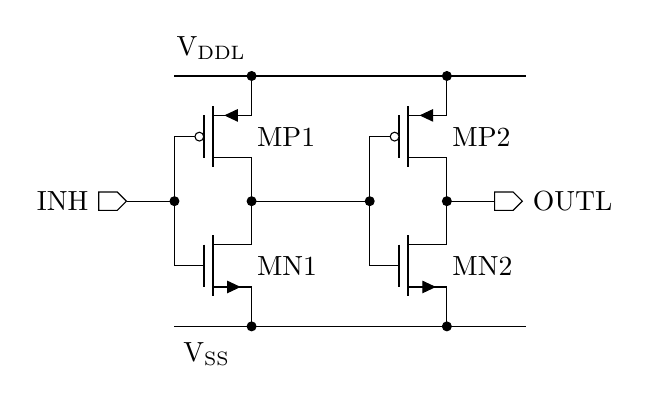
\begin{tikzpicture}[scale=1]
        \ctikzset{tripoles/mos style/arrows}
        \ctikzset{tripoles/pmos style/emptycircle}
        \ctikzset{logic ports=ieee}
        \draw (0,0)
        node[pmos, scale=1](pmos1){MP1}
        (pmos1.D) to [short] ++(0,-0.1) node[nmos, scale=1, anchor=D](nmos1){MN1}
        (pmos1.G) to (nmos1.G)
        ($(pmos1.G)!0.5!(nmos1.G)$) node[circ, scale=1]{} --++ (-0.6,0) node[signal, anchor=east, scale=1, draw](inh){} 
        (inh.west) node[anchor=east, scale=1]{INH}
        ($(pmos1.D)!0.5!(nmos1.D)$) node[circ, scale=1]{} --++(1.5,0) node[circ, scale=1]{}
        (nmos1.center) ++ (1.5,0) node[nmos, scale=1, anchor=G](nmos2){MN2}
        (nmos2.D) to [short] ++(0,0.1) node[pmos, scale=1, anchor=D](pmos2){MP2}
        (nmos2.G) to (pmos2.G)
        ($(pmos2.D)!0.5!(nmos2.D)$) node[circ, scale=1]{} --++ (0.6,0) node[signal, anchor=west, scale=1, draw](outl){}
        (outl.east) node[anchor=west, scale=1]{OUTL}
        (nmos1.G|-nmos1.S) -- (nmos1.S) node[circ, scale=1](vss){} -- (nmos2.S) node[circ, scale=1]{} --++ (1,0)
        (pmos1.G|-pmos1.S) -- (pmos1.S) node[circ, scale=1](vddl){} -- (pmos2.S) node[circ, scale=1]{} --++ (1,0)
	(vss) ++ (-0.15, -0.35) node[left, scale=1]{$\text{V}_\text{SS}$}
	(vddl) ++ (0.05, 0.35) node[left, scale=1]{$\text{V}_\text{DDL}$}
        ;
    \end{tikzpicture}
    \vspace{0.35cm}
    \label{HL_level_shifter}
    }
    \vfil
    \vspace{0.3cm}
    \subfloat[]{
    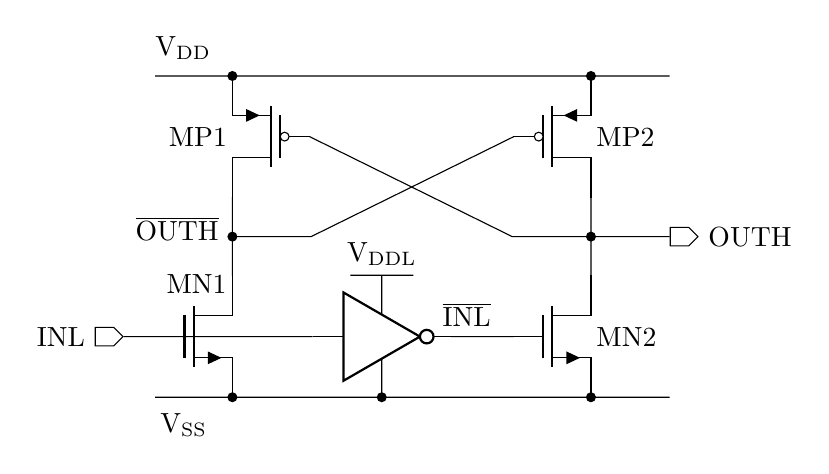
\begin{tikzpicture}[scale=1]
        \ctikzset{tripoles/mos style/arrows}
        \ctikzset{tripoles/pmos style/emptycircle}
        \ctikzset{logic ports=ieee}
        \draw 
        (0,0) node[nmos, anchor=G, scale=1](nmos1){} --++
        (2,0) node[ieeestd not port, anchor=in, scale=1](inv){}
        (nmos1.inner up) ++ (0.05,0.4) node[left, scale=1]{MN1}
        (inv.out) --++ (0.8,0) node[nmos, anchor=G, scale=1](nmos2){MN2} 
        (nmos2.D) --++ (0,0.5) node[circ, scale=1](out){} --++ (0,0.5) node[pmos, anchor=D, scale=1](pmos2){MP2}
        (nmos1.D) --++ (0,0.5) node[circ, scale=1](outb){} --++ (0,0.5) node[pmos, xscale=-1, anchor=D, scale=1](pmos1){\ctikzflipx{MP1}}
        (outb) --++ (1,0) -- (pmos2.G)
        (out) --++ (-1,0) -- (pmos1.G)
        (outb) ++ (-0.05,0.10) node[left, scale=1]{$\overline{\mbox{OUTH}}$}
        (out) --++ (1,0) node[signal, anchor=west, scale=1, draw](out_o){} 
        (out_o.east) node[anchor=west, scale=1]{OUTH}
        (nmos1.G) --++ (-0.4,0) node[signal, anchor=east, scale=1, draw](in){} 
        (in.west) node[anchor=east, scale=1]{INL} 
        (0,0|-nmos1.S) -- (nmos1.S) node[circ, scale=1](vss){} -- (inv.down|-nmos2.S) node[circ, scale=1]{} 
        (inv.down) |- (nmos2.S) node[circ, scale=1]{} --++ (1,0)
        (0,0|-pmos1.S) -- (pmos1.S) node[circ, scale=1](vddh){} -- (pmos2.S) node[circ, scale=1]{} --++ (1,0)
	(vss) ++ (-0.2, -0.35) node[left, scale=1]{$\text{V}_\text{SS}$}
	(vddh) ++ (-0.15, 0.35) node[left, scale=1]{$\text{V}_\text{DD}$}
	(inv.up) --++ (0,0.5) node[above, scale=1](vddl){$\text{V}_\text{DDL}$} ++ (-0.4,0) --++ (0.8,0)
        (inv.out) ++ (0.2,0) node[above, scale=1]{$\overline{\mbox{INL}}$}
        ;
    \end{tikzpicture}
    \label{LH_level_shifter}
    }
    \caption{Шема претварача (а) са високог на низак и (б) са ниског на висок напонски ниво \cite{Osaki:6198744}.}
    \label{Level_shifters}
\end{figure}

Како је напон напајања \DCO-а нижи од остатка система, на управљачке улазе \DCO-a постављени су претварачи са високог на низак напонски ниво \engl[HLLS]{High-Low Level Shifter}, док су на фазне излазе \DCO-a постављени претварачи са ниског на висок напонски ниво \engl[LHLS]{Low-High Level Shifter}. \figurename~\ref{Level_shifters} приказује шеме конвенционалних претварача напонског нивоа који су коришћени у претходно описаном систему. Као што се може видјети са Слике \ref{HL_level_shifter}, претварач са високог на низак напонски ниво није ништа друго до обичан бафер састављен од два инвертора чије напајање ће у коначној реализацији долазити од линије ниског напонског нивоа ($V_\text{DDL}$). \figurename~\ref{LH_level_shifter} приказује шему претварача са ниског на висок напонски ниво, представља регенеративно логичко коло засновано на позитивној повратној спрези~\cite{Osaki:6198744} и састоји се од два унакрсно спрегнута PMOS транзистора (MP1 и MP2) и од NMOS транзистора (MN1 и MN2), који се покрећу преко комплементарних улазних сигнала INL и $\overline{\mbox{INL}}$, гдје је за инвертовање сигнала потребно додати инвертор. \par
С обзиром да је претварач са ниског на висок напонски ниво нешто комплекснији, његов рад ће бити детаљније објашњен. Када напони сигнала INL и $\overline{\mbox{INL}}$ имају вриједност 0 и $V_\text{DDL}$, тада ће MN1 и MN2, редом, бити искључен и укључен. MN2 затим повлачи на нулу напон чвора OUTH, укључујући тако MP1. Тада се и напон чвора $\overline{\mbox{OUTH}}$ подиже на $V_\text{DD}$, MP2 се искључује, а напон на чвору OUTH остаје на нули. С друге стране ако су вриједности напона на INL и $\overline{\mbox{INL}}$ једнаки $V_\text{DDL}$ и 0, тада ће MN1 и MN2 бити укључен и искључен, респективно. MN1 тада повлачи на нулу напон чвора $\overline{\mbox{OUTH}}$, укључујући тако MP2, чиме се напон OUTH подиже на $V_\text{DD}$, а MP1 се искључује. \par
Треба запазити да је напон чвора OUTH одређен покретачком струјом \engl{Drive Current} транзисторa MP2 и MN2, тј. струјом која тече кроз канал транзистора када су укључени. Зато, ако је покретачка струја кроз транзистор MP2 много већа него кроз MN2, тада OUTH не може бити испражњен што доводи до тога да претварач не може исправно радити у таквим ситуацијама~\cite{Osaki:6198744}. До њих иначе може доћи ако је разлика између $V_\text{DD}$ и $V_\text{DDL}$ превелика, што у примјени из овог рада није случај. \par
Претварачи напонских нивоа могу утицати на фактор испуњености импулса тј. периоде такта \engl{Duty Cycle}, поготово на излазу претварача са ниског на висок напонски ниво. Међутим, то се углавном може избјећи додатним баферовањем излаза \DCO-а тј. физичким уметањем одговарајућих бафера између фазног излаза \DCO-a и претварача напонског нивоа чиме се фактор испуњености импулса такта може приближити идеалној вредности од 50\,\%, како би такав дошао на улаз претварача са ниског на висок напонски ниво.


\section{Имплементација и резултати симулација} \label{Implementation and results}
У овом поглављу биће приказана имплементација система кроз анализу SystemVerilog кода и хијерархијским приказом лејаута комплетног \FLL-a. Затим ће бити приказани резултати симулација у различитим условима након екстракције паразитних капацитивности. Такође ће бити приказани резултати софтверског модела рада \FLL-a, а биће направљено и поређење два \DCO-а имплементирана у 2 различите технологије. Дигитални \FLL\ описан у овом раду, имплементиран је коришћењем SystemVerilog језика за опис хардвера у 130\,nm CMOS технологији. Улазни референтни такт је 16\,MHz, док се такт \DCO-a подешава до 640\,MHz, при чему је резолуција учестаности око 2,8\,MHz у типичним условима рада. 

\subsection{SystemVerilog код} \label{section:impl:systemVerilog}
У овом поглављу биће приказани најбитнији дијелови имплементације \FLL-а на нивоу SystemVerilog~\cite{SystemVerilog:1800-2023} језика за опис хардвера. Уз поједине дијелове кода ће бити објашњења у сврху лакшег разумијевања. \lstlistingname~\ref{lst:sv:fll_input} приказује улазе и излазе \FLL-a, који су побројани и у поглављу~\ref{FLL structure}, са додатим сигналима за подешавање управљачке логике. \par 
\begin{lstlisting}[language=Verilog, caption={Улазни и излазни сигнали хијерархијски највишег \FLL\ модула.}, label={lst:sv:fll_input}]
 // Frequency-locked loop
module fll #(
  parameter integer CW = 8  // frequency control word width
)(
  /////////////////////
  // Clock and reset //
  /////////////////////
  input           clk_ref_i,       // [0] reference clock @ 32MHz
  input           clk_ref_en_i,    // [1] reference clock enable signal
                                   //     0: reference clock propagation disabled
                                   //     1: reference clock propagation enabled
  input           rst_ni,          // [0] async reset
                                   //     0: active/asserted
                                   //     1: inactive/deasserted
  /////////
  // FLL //
  /////////
  input  [CW-1:0] clk_mult_i,      // [0d20] reference frequency multiplier (or frequency control word)
                                   //        20 * 32MHz = 640MHz
  /////////
  // DCO //
  /////////
  input           dco_pwr_sel_i,   // [1]     DCO clock output power supply selection
                                   //         0: FLL uses DCO clock output @ VDDL (~1.1V,     adjustable)
                                   //         1: FLL uses DCO clock output @ VDD  (~1.2V, non-adjustable)
  input     [1:0] dco_ctrl_mode_i, // [1]     DCO control mode
                                   //         0d0: FIXED     - DCO control word is internally set to 0d203
                                   //         0d1: MANUAL    - DCO control word is set via "dco_ctrl_man_i" register
                                   //         0d2: BANG-BANG - DCO control word is set by a comparator and a counter
                                   //         0d3: PID       - DCO control word is PID regulated
  input  [CW-1:0] dco_ctrl_man_i,  // [0d200] DCO control word value for MANUAL mode
                                   //         In simulation in typical conditions, a value around 0d200 achieved 640MHz,
                                   //         a value of 0 achieved ~42MHz and a value of 0d255 achieved ~764MHz
  /////////
  // PID //
  /////////
  input  [CW-1:0] pid_kp_i,        // [0b01000000] PID controller proportional constant
                                   //              A signed number in Q6.2 format (0b010000_00 == 0d16)
  input  [CW-1:0] pid_ki_i,        // [0b01000000] PID controller integral constant
                                   //              A signed number in Q6.2 format (0b010000_00 == 0d16)
  input  [CW-1:0] pid_kd_i,        // [0]          PID controller derivative constant
                                   //              A signed number in Q6.2 format
  /////////
  // FLL //
  /////////
  input     [3:0] lock_cnt_i,      // [0b1000] FLL internal counter lock condition threshold
  output          lock_o,          // [0]      FLL lock signal - indicates if FLL achieved the target frequency
                                   //          0: the FLL did not its target frequency yet
                                   //          1: the FLL achieved its target frequency
  ////////////////
  // OSC output //
  ////////////////
  output        clk_dco_o          // DCO clock - one phase
);
...
endmodule
\end{lstlisting}
У поглављу~\ref{section:control_preprocessing} описана је улога и начин рада управљачке предобраде, а~\lstlistingname~\ref{lst:sv:cnt_gray} приказује хардверску имплементацију Грејевог бројача и начин како се генеришу узастопне вриједности бројача. Као што се из кода може видјети, оне се генеришу из наредне природне бинарне вриједности тако што се најстарији бит задржава, док су остали битови резултат бит по бит ексклузивно ИЛИ \engl{XOR} операције између свих битова осим најмлађег и свих битова осим најстаријег (линија \prog{22} у Листингу~\ref{lst:sv:cnt_gray}). Рецимо ако је наредна природна вриједност бројача 5 (бинарно 00000101, ако је ширина бројача 8), да би се претворила у Грејев код, задржава се најстарији бит, тј. 0, а осталих седам се додаје као резултат поменуте ексклузивно ИЛИ операције, тј. 0000010\,\^\,0000101, што даје вриједност 0000111 коју треба додати на 0, чиме се добија вриједност 00000111, која, ако погледамо Табелу~\ref{gray_code}, одговара природној вриједности 5. \par
\begin{lstlisting}[language=Verilog, caption={Модул Грејевог бројача.}, label={lst:sv:cnt_gray}]
module cnt_gray #(
  parameter int  W   = 8,
  parameter byte Val = W'(0)
)(
  input          clk_i,
  input          rst_ni,
  input          en_i,
  output [W-1:0] cnt_gray_o
);

  logic [W-1:0] cnt_bin;
  logic [W-1:0] cnt_bin_next;
  logic [W-1:0] cnt_gray;
  assign cnt_bin_next = cnt_bin + W'(1);
  always_ff @(posedge clk_i or negedge rst_ni) begin
    if (!rst_ni) begin
      cnt_bin <= Val;
      cnt_gray <= {Val[W-1], Val[W-1:1] ^ Val[W-2:0]};
    end else begin
      if (en_i) begin
        cnt_bin <= cnt_bin_next;
        cnt_gray <= {cnt_bin_next[W-1], cnt_bin_next[W-1:1] ^ cnt_bin_next[W-2:0]};
      end else begin
        cnt_bin <= Val;
        cnt_gray <= {Val[W-1], Val[W-1:1] ^ Val[W-2:0]};
      end
    end
  end
  assign cnt_gray_o = cnt_gray;

endmodule
\end{lstlisting}
Добијена вриједност у Грејевом коду се синхронизује кроз два флип флопа и претвара се у природну бинарну вриједност, а имплементација тога је унутар \prog{fll} модула и дата је у~\lstlistingname{у}~\ref{lst:sv:fll_sync_gray_to_bin}. Узоркована вриједност Грејевог бројача је на магистрали \prog{cnt\_dco\_gray\_q2}, док је природна бинарна вриједност на магистрали \prog{cnt\_dco} и она суштински представља тренутни умножак учестаности добијене на излазу \DCO-a, и представља податак спреман за поређење са жељеним умношком са улаза, унутар блока управљачке логике. Сваки бит у тој магистали се добија као резултат логичке XOR операције над свим битовима Грејевог записа, помјереног онолико мјеста удесно колико износи тежина тренутног бита у \prog{cnt\_dco} магистрали (имплементација на линији \prog{7} у \lstlistingname{у}~\ref{lst:sv:fll_sync_gray_to_bin}). \par
\begin{lstlisting}[language=Verilog, caption={Претварање Грејевог кода у природну бинарну вриједност.}, label={lst:sv:fll_sync_gray_to_bin}]
module fll #(
  ...
  // Gray to binary conversion
  genvar i;
  generate
    for(i=0; i<CW; i++) begin: gen_gray2bin_conv
       assign cnt_dco[i] = ^(cnt_dco_gray_q2 >> i);
    end: gen_gray2bin_conv
  endgenerate
  ...
endmodule
\end{lstlisting}
Двостепени регулатор, као један дио управљачке логике, је подробније објашњен у поглављу~\ref{section:bang_bang}. Као што је тамо напоменуто, састоји се од компаратора и једног бројача. Компаратор служи за поређење добијеног и жељеног умношка учестаности, а резултат се шаље у бројач који на основи њега одређује како подесити управљачку ријеч за \DCO. \lstlistingname~\ref{lst:sv:bang_bang:comparator} приказује компараторски дио који се налази унутар \prog{fll} модула. Као што се може закључити, \prog{cnt\_dco\_q} представља семпловану вриједност тренутног умношка, односно вриједност \prog{cnt\_dco} из \lstlistingname{a}~\ref{lst:sv:fll_sync_gray_to_bin}. Сигнал \prog{cnt\_ref\_up\_dn} одређује да ли инкрементирати или декрементирати управљачку ријеч \DCO-а, док сигнал \prog{cnt\_ref\_en} одређује да ли уопште мијењати вриједност бројача (сигнал \prog{lock\_o} ће бити поменут при анализи имплементације \PID\ регулатора). Закључује се да се поменути сигнали прослјеђују даље у блок бројача, чија је имплементација, као посебног \prog{cnt} модула, приказана у \lstlistingname{у}~\ref{lst:sv:bang_bang:cnt}. Сигнали \prog{cnt\_ref\_up\_dn} и \prog{cnt\_ref\_en} се при инстанцирању \prog{cnt} модула прослијеђују на његове \prog{up\_down\_i} и \prog{en\_i} улазе, респективно. \par
\begin{lstlisting}[language=Verilog, caption={Компараторски дио двостепеног регулатора.}, label={lst:sv:bang_bang:comparator}]
module fll #(
  ...
  // Comparator
  logic  cnt_ref_up_dn;
  logic  cnt_ref_en;
  assign cnt_ref_up_dn = (clk_mult_i >= cnt_dco_q) ?    1'b1 : 1'b0;
  assign cnt_ref_en    = (clk_mult_i != cnt_dco_q) ? ~lock_o : 1'b0;
  ...
endmodule
\end{lstlisting}
\begin{lstlisting}[language=Verilog, caption={Имплементација бројача из двостепеног регулатора.}, label={lst:sv:bang_bang:cnt}]
// Up-down counter with enable
module cnt #(
  parameter int  W   = 8,     // count width (number of bits)
  parameter byte Val = W'(0)  // counter default value
) (
  // Clock and reset
  input                clk_i,     // clock
  input                rst_ni,    // async reset
  // Control
  input                en_i,      // enables counting
  input                up_down_i, // count direction
  // Count data output
  output logic [W-1:0] cnt_o      // count output
);

always_ff @(posedge clk_i or negedge rst_ni) begin
  if (!rst_ni) begin
    cnt_o <= Val;
  end else begin
    if (en_i) begin
      if (up_down_i == 1'b1) begin
        cnt_o <= W'(cnt_o + W'(1));
      end else begin
        cnt_o <= W'(cnt_o - W'(1));
      end
    end else begin
      cnt_o <= cnt_o;
    end
  end
end

endmodule
\end{lstlisting}
Имплементација \PID\ регулатора, детаљније објашњеног у поглављу~\ref{section:pid}, приказана је у \lstlistingname{у}~\ref{lst:sv:pid}, гдје се види да је имплементиран као посебан \prog{pid} модул. Поред улаза такта, ресета и коефицијената регулатора, ту су још улази:
\begin{itemize}
	\item \prog{setpoint\_i} који представља жељени умножак учестаности (при инстанцирању модула прослјеђује му се вриједност \prog{clk\_mult\_i} са улаза \prog{fll} модула),
	\item \prog{feedback\_i} који представља семпловани тренутни умножак (при инстанцирању модула прослјеђује му се семплована вриједност \prog{cnt\_dco} из \lstlistingname{a}~\ref{lst:sv:fll_sync_gray_to_bin}) и
	\item \prog{lock\_cnt\_i} који означава колико узлазних ивица такта грешка мора бити једнака нули да би се достигло закључавање, односно да би се излазни сигнал \prog{lock\_o} подигао на 1.
\end{itemize}
Излаз \prog{ctrl\_o} представља податак који ће да служи као управљачка ријеч за DCO (аналогно излазу \prog{cnt\_o} из \prog{cnt} модула двостепеног регулатора). Он означава 8-битну цјелобројну вриједност и добија се издвајањем 8 бита од позиције 13 до позиције 6 из промјенљиве \prog{ctrl\_pid} (линија \prog{64} у \lstlistingname{у}~\ref{lst:sv:pid}) у којој је смјештена сума пропорционалног, интегралног и диференцијалног дејства. Такво издвајање битова је резултат коришћења бинарног бројевног система са фиксном тачком, о коме се више може наћи у литератури~\cite{Harris:DIGITAL_DESIGN_2012}, а све то у сврху повећања резолуције подешавања \PID\ регулатора. Наиме, улазни коефицијенти \prog{kp\_i}, \prog{ki\_i} и \prog{kd\_i} су 8-битни у формату Q6.2 (6 бита за цјелобројни дио, 2 за децимални дио), док је формат \prog{ctrl\_pid} промјенљиве Q12.6 (12 битова за цјелобројни дио, 6 за децимални дио), па се поменутим одсијецањем врши заокруживање на 8-битни цијели број. \par
\begin{lstlisting}[language=Verilog, caption={Имплементација \PID\ регулатора.}, label={lst:sv:pid}]
// PID controller
module pid #(
  parameter int DW = 8,  // data input width
  parameter int CW = 8   // control output width
) (
  input                 clk_i,
  input                 rst_ni,
  input        [DW-1:0] kp_i,
  input        [DW-1:0] ki_i,
  input        [DW-1:0] kd_i,
  input        [DW-1:0] setpoint_i,
  input        [DW-1:0] feedback_i,
  input        [3:0]    lock_cnt_i,
  output logic [CW-1:0] ctrl_o,
  output logic          lock_o
);

  // Localparam
  localparam int ErrCntW = 4;

  // Error logic
  logic signed [DW-1:0] err;
  logic signed [DW-1:0] err_prev;
  logic signed [DW-1:0] err_diff;
  assign err = setpoint_i - feedback_i;
  assign err_diff = err - err_prev;
  logic [ErrCntW-1:0] err_eq0_cnt;
  logic [ErrCntW-1:0] err_cnt_lock;
  assign err_cnt_lock = ErrCntW'(lock_cnt_i);
  always_ff @(posedge clk_i or negedge rst_ni) begin
    if (!rst_ni) begin
      err_eq0_cnt   <= '0;
    end else begin
      if ((err == '0) && (err_eq0_cnt < err_cnt_lock)) begin
        err_eq0_cnt <= err_eq0_cnt + ErrCntW'(1);
      end
    end
  end

  // PID calculation & lock
  logic signed [CW+DW-1:0] prop;
  logic signed [CW+DW  :0] integ;
  logic signed [CW+DW-1:0] deriv;
  logic signed [CW+DW+1:0] ctrl_pid;
  always_ff @(posedge clk_i or negedge rst_ni) begin
    if (!rst_ni) begin
      prop     <= '0;
      integ    <= '0;
      deriv    <= '0;
      err_prev <= '0;
      ctrl_pid <= '0;
      lock_o   <= '0;
    end else begin
      prop     <= (kp_i * err);
      integ    <= integ + (ki_i * err);
      deriv    <= (kd_i * err_diff);
      err_prev <= err;
      if ((err == '0) && (err_eq0_cnt == err_cnt_lock) && (err_cnt_lock != '0)) begin
        lock_o <= 1'b1;
      end
      ctrl_pid <= lock_o ? ctrl_pid : 18'(prop) + integ + 18'(deriv);
    end
  end
  assign ctrl_o = ctrl_pid[13:6];

endmodule
\end{lstlisting}
Излази \prog{cnt\_o} и \prog{ctrl\_o} из двостепеног и \PID\ регулатора, редом, представљају суштински број тростатичких инвертора \DCO-а који требају бити укључени, што утиче на његову излазну учестаност. Међутим, та вриједност се не прослјеђује директно у модул \DCO-a, већ се преко управљачког декодера анализираног у поглављу~\ref{section:control_decoder} претвара у скуп одговарајућих векторских улаза за управљање \DCO-ом тј. редовима и колонама тростатичких инвертора унутар њега. Тај поступак претварања је приказан у \lstlistingname{у}~\ref{lst:sv:control_decoder}, а имплементиран је у оквиру \prog{fll} модула. \par
\begin{lstlisting}[language=Verilog, caption={Имплементација управљачког декодера из поглавља~\ref{section:control_decoder}.}, label={lst:sv:control_decoder}]
module fll #(
  ...
  // Convert digital code to real DCO inputs (row/col sel and row on)
  localparam int NumRows = 17;
  localparam int NumCols = 15;
  logic [NumRows-1:0] row_on_d;
  logic [NumRows-1:0] row_sel_d;
  logic [NumCols-1:0] col_sel_d;
  always_comb begin
      row_on_d  = '0;
      row_sel_d = '0;
      col_sel_d = '0;
      for(int r = 1; r <= NumRows; r = r + 1) begin
        // Row on logic
        if (int'(dco_ctrl) > r*NumCols) begin
          row_on_d[r-1] = 1'b1;
        end else begin
          row_on_d[r-1] = 1'b0;
        end
        // Row & column select logic
        if ((int'(dco_ctrl) > (r-1)*NumCols) && (int'(dco_ctrl) <= r*NumCols)) begin
          for(int c = 0; c < NumCols; c = c + 1) begin
            if ((r-1)*NumCols + c < int'(dco_ctrl)) begin
              col_sel_d[c] = 1'b1;
            end else begin
              col_sel_d[c] = 1'b0;
            end
          end
          row_sel_d[r-1] = 1'b1;
        end else begin
          row_sel_d[r-1] = 1'b0;
        end
      end
  end
  ...
endmodule
\end{lstlisting}
Сигнали \prog{row\_on\_d}, \prog{row\_sel\_d} и \prog{col\_sel\_d} се синхронизују на одговарајући такт и прослјеђују се као улази у \DCO\ модул који је имплементиран као посебан блок у алатима за аналогно пројектовање, па стога овдје нема свој опис у SystemVerilog-у, већ се тај блок само инстанцира унутар \prog{fll} модула, као што је приказано у \lstlistingname{у}~\ref{lst:sv:dco_inst}. Као што се може видјети, \prog{dco} модул садржи излазе за свих 5 фаза на ниском ($V_\text{DDL}$) и високом ($V_\text{DD}$) напонском нивоу, а који од та два напонска нивоа ће се наћи на \prog{clk\_dco\_o} излазу \prog{fll} модула одређује његов улазни сигнал \prog{dco\_pwr\_sel\_i} (погледати \lstlistingname~\ref{lst:sv:fll_input}). \par 
\begin{lstlisting}[language=Verilog, caption={Инстанцирање \DCO\ блока.}, label={lst:sv:dco_inst}]
module fll #(
  ...
  // DCO model
  logic clk_dco_ph0;
  logic clk_dco_ph0_l;
  logic clk_dco_ph0_h;
  logic clk_dco_ph1;
  logic clk_dco_ph1_l;
  logic clk_dco_ph1_h;
  logic clk_dco_ph2;
  logic clk_dco_ph2_l;
  logic clk_dco_ph2_h;
  dco u_dco(
    .ROW_ON    (row_on),
    .ROW_SEL   (row_sel),
    .COLUMN_SEL(col_sel),
    .PH0       (clk_dco_ph0_h),
    .PH0_L     (clk_dco_ph0_l),
    .PH1       (clk_dco_ph1_h),
    .PH1_L     (clk_dco_ph1_l),
    .PH2       (clk_dco_ph2_h),
    .PH2_L     (clk_dco_ph2_l),
    .PH3       (),
    .PH3_L     (),
    .PH4       (),
    .PH4_L     ()
  );
  assign clk_dco_ph0 = dco_pwr_sel_i ? clk_dco_ph0_h : clk_dco_ph0_l;
  assign clk_dco_ph1 = dco_pwr_sel_i ? clk_dco_ph1_h : clk_dco_ph1_l;
  assign clk_dco_ph2 = dco_pwr_sel_i ? clk_dco_ph2_h : clk_dco_ph2_l;
  assign clk_dco_o = clk_dco_ph2;
  ...
endmodule
\end{lstlisting}

\subsection{Лејаут}
За израду лејаута намјенски је коришћена 7Т \engl{7-Track} библиотака стандардних ћелија, гдје 7Т означава да висина свих ћелија тачно толике висине да може да се вертикално провуче 7 линија метала минималне ширине и са минималним размаком. То доприноси лакшем аутоматском (а и ручном) рутирању и слагању ћелија у компактну цјелину у сврху оптималне искористивости простора. Лејаут коначне верзије цјелокупног \FLL-а приказан је на Слици~\ref{layout_FLL}. Читав дизајн \FLL-a заузима 33000\,\text\textmu m$^\text2$. Компонента у доњем десном углу је дигитално контролисани осцилатор, док остатак лејаута углавном припада управљачкој логици \FLL-a. \par
\begin{figure}[!ht]
	 \centering
	 \begin{tikzpicture}
	 % The image node
        \node[inner sep=0] (layout_FLL) { 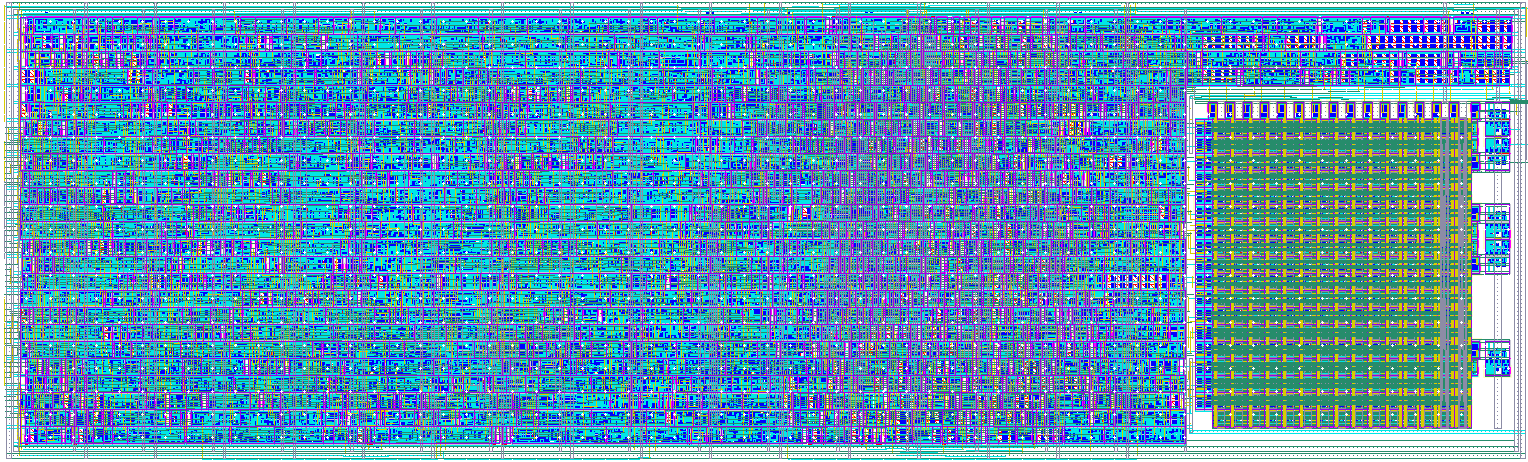
\includegraphics[scale=0.37]{slike/layout_FLL.png} };
        \draw[<->] (-7.75,-2.25) -- (-7.7,2.25) node[midway, left=0.2, above=0.05, rotate=90] {\footnotesize 100\,\textmu m};
        \draw[<->] (-7.45,-2.55) -- (7.45,-2.55) node[midway, right=0.1, below=0.02] {\footnotesize 330\,\textmu m};
        \end{tikzpicture}	
	\caption{Лејаут дигиталног \FLL-а, са \DCO-ом у доњем десном углу.}
	\label{layout_FLL}
\end{figure}
\DCO\ је имплементиран као независна компонента коришћењем библиотека стандардних ћелија. Од читавог лејаута \FLL-a, око 13\,\% заузима \DCO, тачније око 4300\,\text\textmu m$^\text2$ (вриједност добијена сабирањем појединачних површина коришћених ћелија). \figurename~\ref{layout_dco5_130} приказује лејаут \DCO-a са претварачима напонских нивоа који се могу уочити са лијеве и горње стране лејаута (претварачи са високог на низак напонски ниво на управљачким улазима \DCO-a), као и са десне стране (претварачи са ниског на висок напонски ниво на свих 5 фаза \DCO-a). \par 
\begin{figure}[!ht]
	 \centering
	 \vspace{-0.3cm}
	 \begin{tikzpicture}
	 % The image node
        \node[inner sep=0] (layout_dco5_130) { 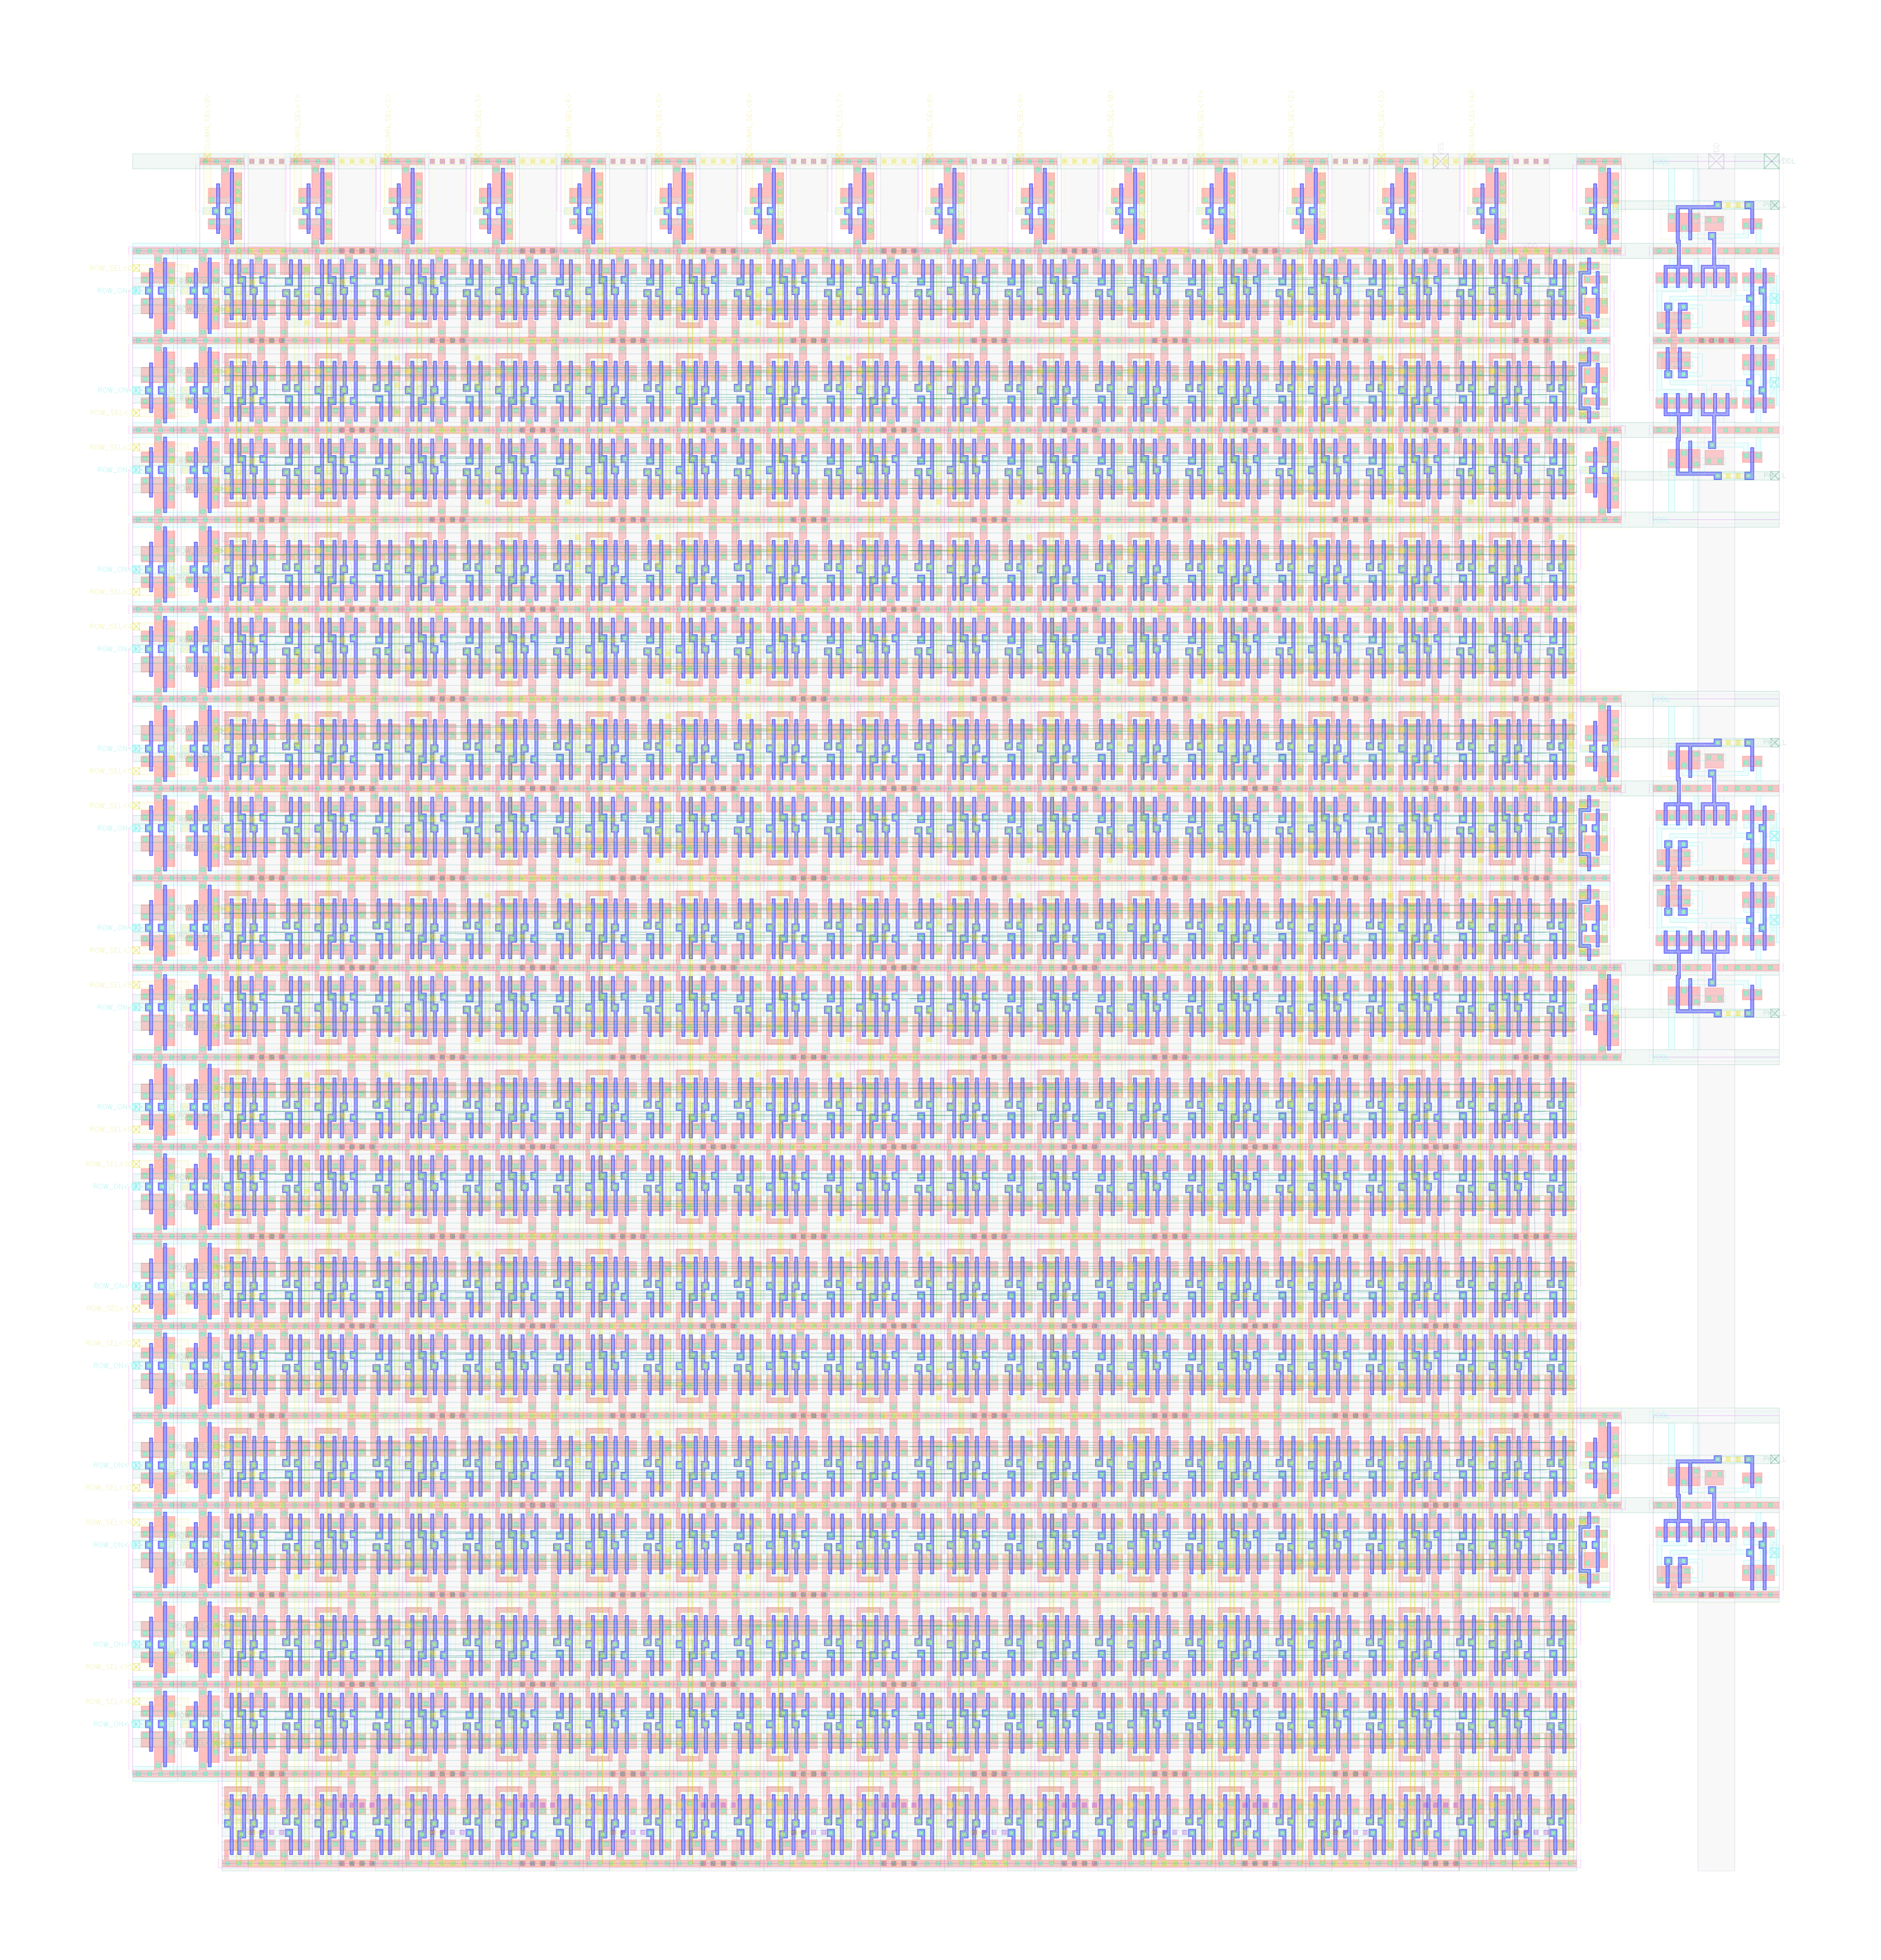
\includegraphics[scale=0.15]{slike/layout_dco5_hl_lh_130.png} };
        \draw[<->] (-7.25,-7.3) -- (-7.25,6.8) node[midway, left=0.2, above=0.05, rotate=90] {\footnotesize 70,11\,\textmu m};
        \draw[<->] (-6.73,-7.9) -- (7,-7.9) node[midway, right=0.1, below=0.02] {\footnotesize 67,825\,\textmu m};
        \end{tikzpicture}	
	\caption{Лејаут \DCO-а са претварачима напонских нивоа.}
	\label{layout_dco5_130}
\end{figure}
\figurename~\ref{layout_dco_cell} приказује лејаут једне ћелије \DCO-a. Са десне стране ћелије је оријентисан тростатички инвертор, док је са лијеве стране управљачки И-ИЛИ дио. Површина једне ћелије је око 13,7\,\text\textmu m$^\text2$. \par
%\begin{figure}[!ht]
%	 \centering
%	 \begin{tikzpicture}
%	 % The image node
%        \node[inner sep=0] (layout_dco_cell) { 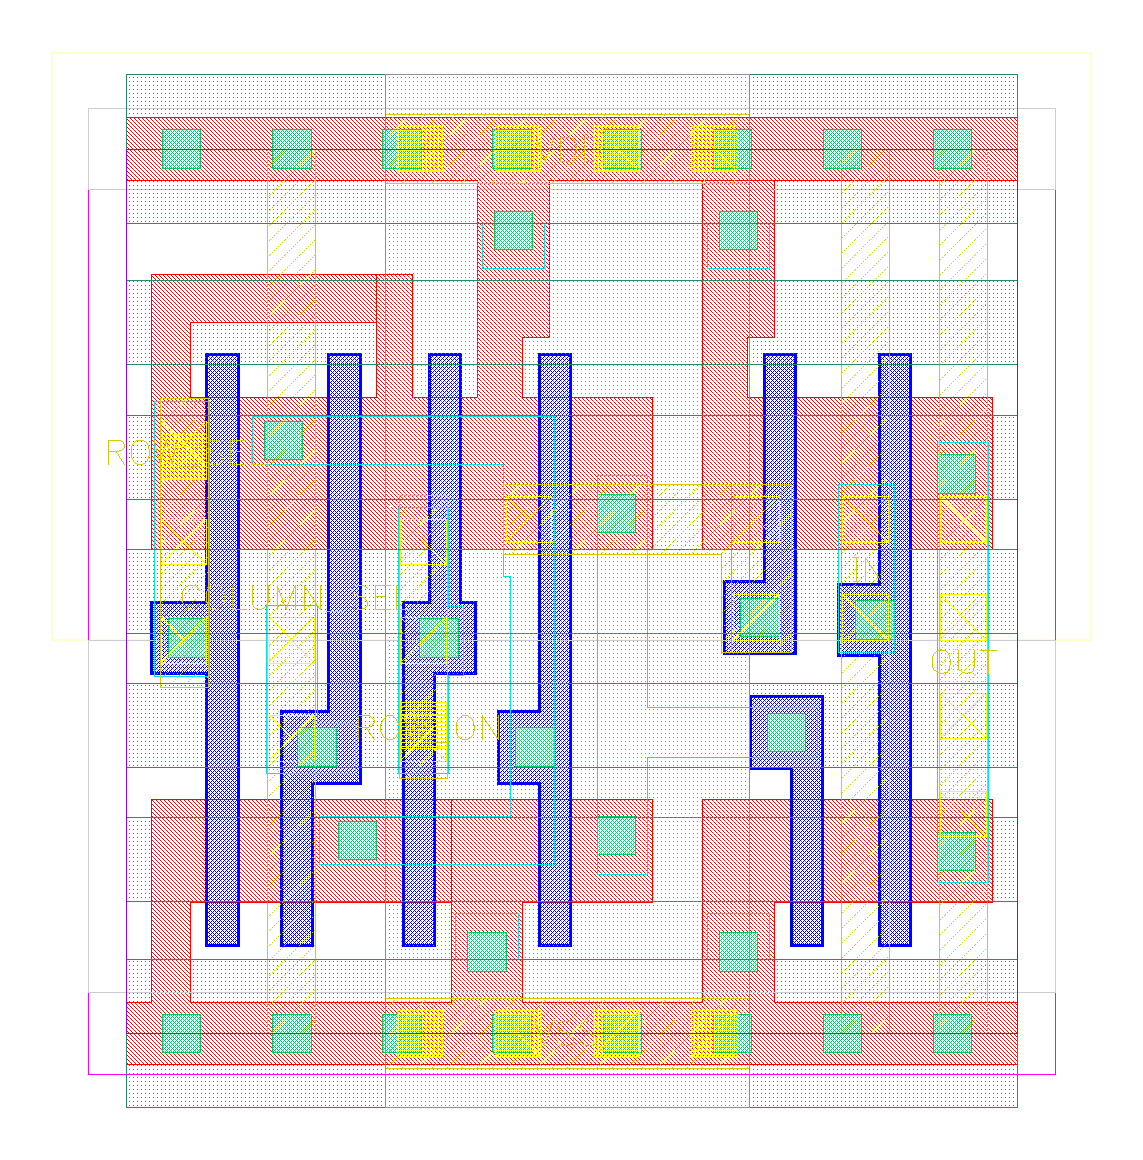
\includegraphics[scale=0.25]{slike/layout_dco_cell.png} };
%        \draw[<->] (-3.5,-3.1) -- (-3.5,2.9) node[midway, left=0.2, above=0.05, rotate=90] {\footnotesize 3.69\,\textmu m};
%        \draw[<->] (-3.0,-3.8) -- (3.0,-3.8) node[midway, right=0.1, below=0.02] {\footnotesize 3.72\,\textmu m};
%        \end{tikzpicture}	
%	\caption{Лејаут ћелије \DCO-а.}
%	\label{layout_dco_cell}
%\end{figure}
Лејаут претварача са високог на низак и са ниског на висок напонски ниво је приказан на Слици~\ref{layout_lvl_hl} и~\ref{layout_lvl_lh}, респективно. Као што је већ напоменуто у поглављу~\ref{LS chapter}, претварач са високог на низак напонски ниво је у суштини бафер и овдје је његова површина око 6,8\,\text\textmu m$^\text2$, док је претварач са ниског на висок напонски ниво нешто сложенији и, ради бољег уклапања тј. заузимања мање површине у комбинацији са \DCO-ом, имплементиран је као ћелија са дуплом висином, што омогућава мању ширину ћелије, а површина јој је око 38,3\,\text\textmu m$^\text2$. \par 
%\begin{figure}[!ht]
%	 \centering
%	 \subfloat[\centering]{
%	 	\begin{tikzpicture}
%	 	% The image node
%        	\node[inner sep=0] (layout_lvl_hl) { 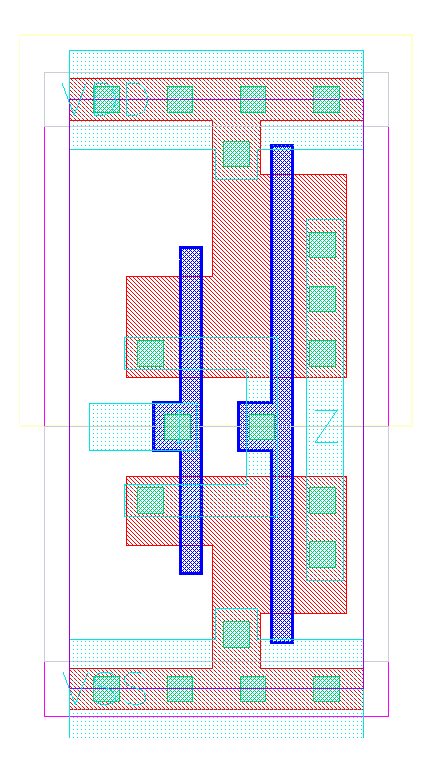
\includegraphics[scale=0.27]{slike/layout_lvl_hl.png} };
%        	\draw[<->] (-1.62,-2.16) -- (-1.62,2.05) node[midway, left=0.2, above=0.05, rotate=90] {\footnotesize 3.69\,\textmu m};
%        	\draw[<->] (-1.08,-2.8) -- (1.08,-2.8) node[midway, right=0.1, below=0.02] {\footnotesize 1.84\,\textmu m};
%        	\end{tikzpicture}
%		\label{layout_lvl_hl}}
%	\qquad
%	\hspace{1cm}
%	\subfloat[\centering]{
%	 	\begin{tikzpicture}
%	 	% The image node
%        	\node[inner sep=0] (layout_lvl_lh) { 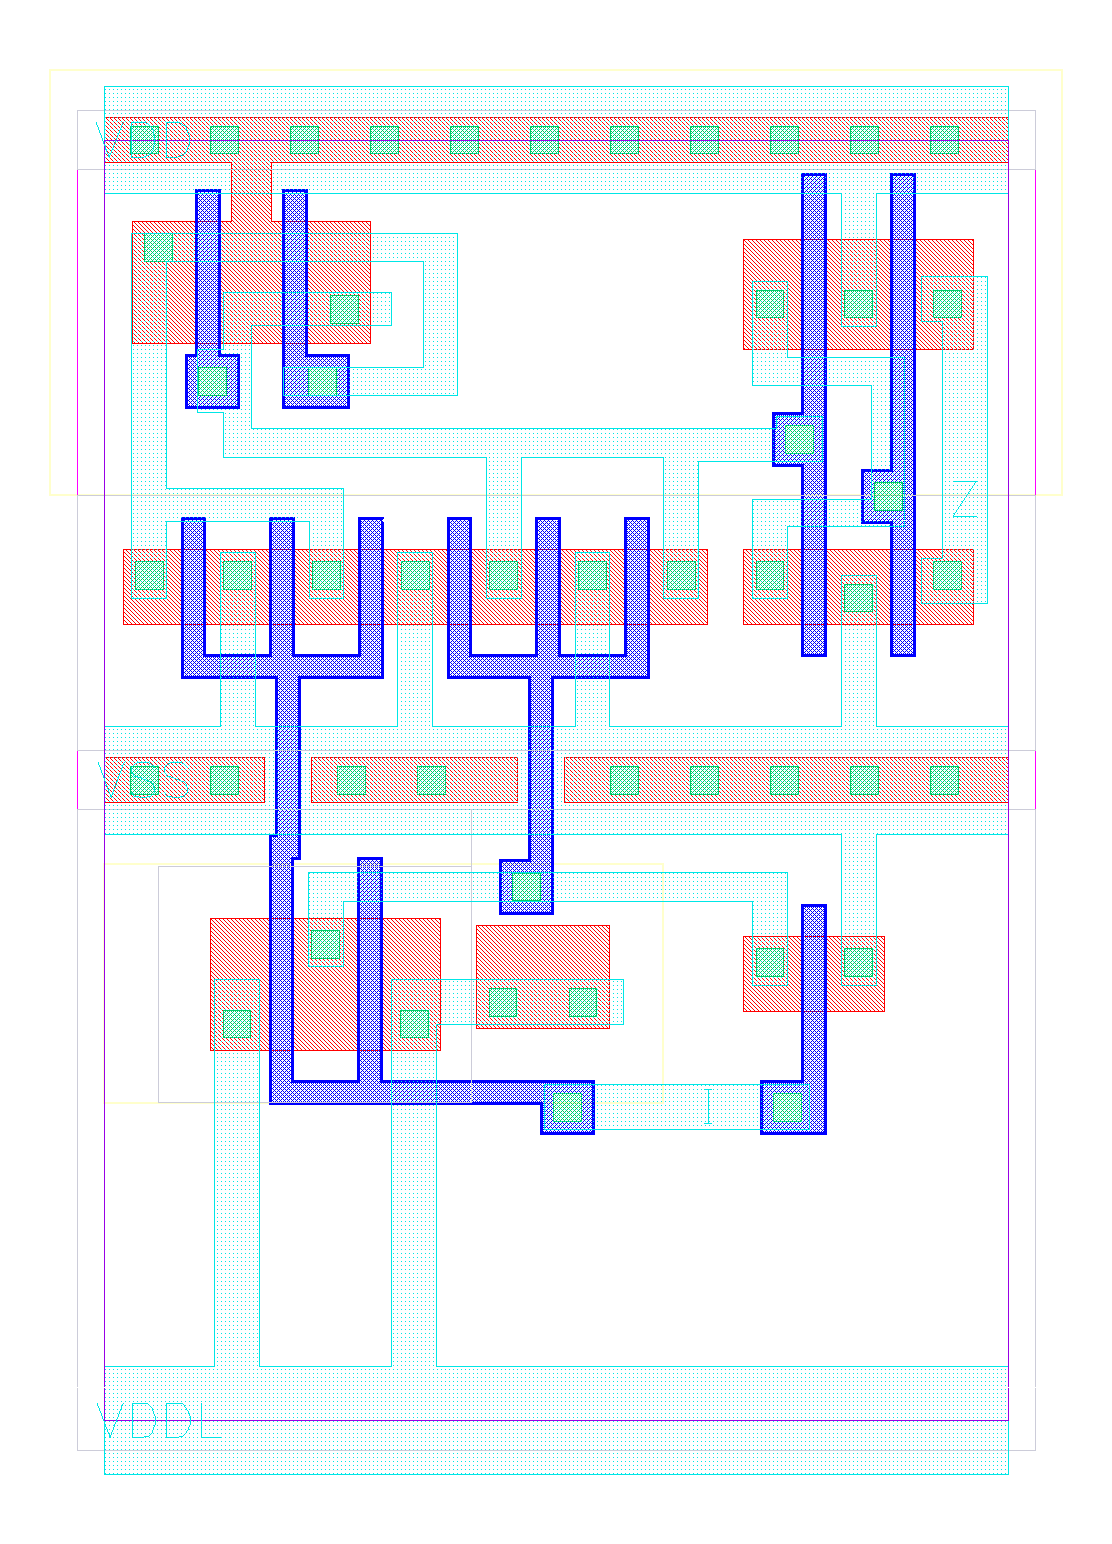
\includegraphics[scale=0.25]{slike/layout_lvl_lh.png} };
%        	\draw[<->] (-3.5,-4.3) -- (-3.5,4.1) node[midway, left=0.2, above=0.05, rotate=90] {\footnotesize 7.38\,\textmu m\,(2$\cdot$3.69\,\textmu m)};
%        	\draw[<->] (-3.1,-4.9) -- (3.1,-4.9) node[midway, right=0.1, below=0.02] {\footnotesize 5.195\,\textmu m};
%        	\end{tikzpicture}
%		\label{layout_lvl_lh}}
%	\caption{Лејаут претварача са (а) високог на низак и (б) ниског на висок напонски ниво.}
%	\label{layout_lvl_hl_lh}
%\end{figure}
\begin{figure}[!ht]
	 \centering
	 \subfloat[\centering]{
	 	\begin{tikzpicture}
	 	% The image node
        	\node[inner sep=0] (layout_dco_cell) { 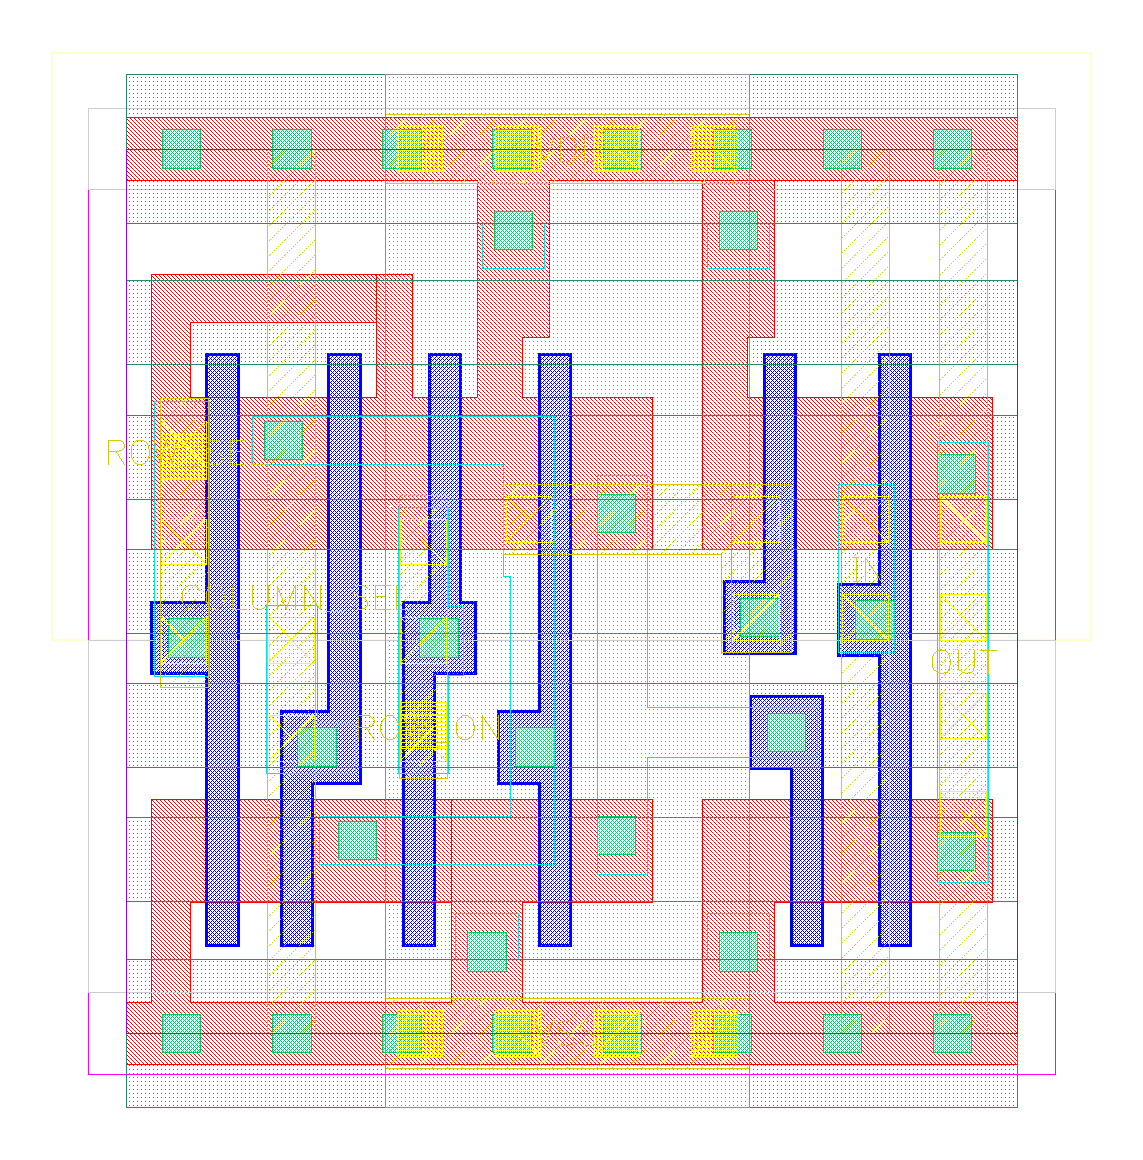
\includegraphics[scale=0.167]{slike/layout_dco_cell.png} };
        	\draw[<->] (-2.3,-2) -- (-2.3,1.9) node[midway, left=0.2, above=0.05, rotate=90] {\footnotesize 3,69\,\textmu m};
        	\draw[<->] (-1.95,-2.6) -- (1.95,-2.6) node[midway, right=0.1, below=0.02] {\footnotesize 3,72\,\textmu m};
        	%\draw[<->] (-3.5,-3.1) -- (-3.5,2.9) node[midway, left=0.2, above=0.05, rotate=90] {\footnotesize 3.69\,\textmu m};
        	%\draw[<->] (-3.0,-3.8) -- (3.0,-3.8) node[midway, right=0.1, below=0.02] {\footnotesize 3.72\,\textmu m};
        	\end{tikzpicture}	
		\label{layout_dco_cell}}
	 \qquad
	 \hspace{-1.3cm}
	 \subfloat[\centering]{
	 	\begin{tikzpicture}
	 	% The image node
        	\node[inner sep=0] (layout_lvl_hl) { 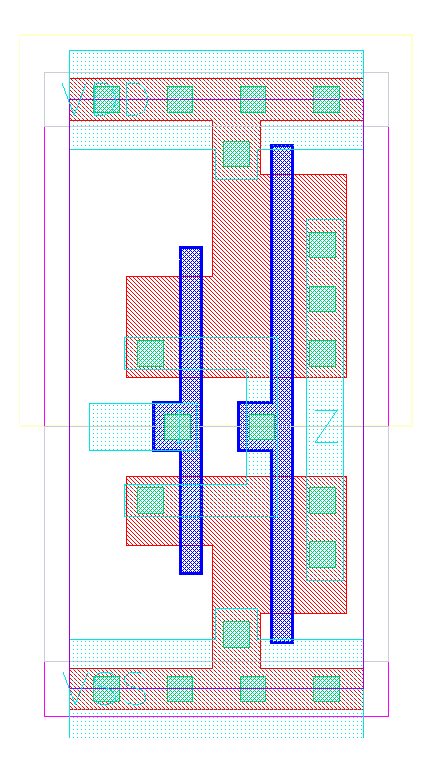
\includegraphics[scale=0.25]{slike/layout_lvl_hl.png} };
        	\draw[<->] (-1.3,-2) -- (-1.3,1.9) node[midway, left=0.2, above=0.05, rotate=90] {\footnotesize 3,69\,\textmu m};
        	\draw[<->] (-0.95,-2.6) -- (0.95,-2.6) node[midway, right=0.1, below=0.02] {\footnotesize 1,84\,\textmu m};
        	\end{tikzpicture}
		\label{layout_lvl_hl}}
	\qquad
%	\hspace{1cm}
	\hspace{-1.3cm}
	\subfloat[\centering]{
		%\vspace{0.3cm}
	 	\begin{tikzpicture}
	 	% The image node
        	\node[inner sep=0] (layout_lvl_lh) { 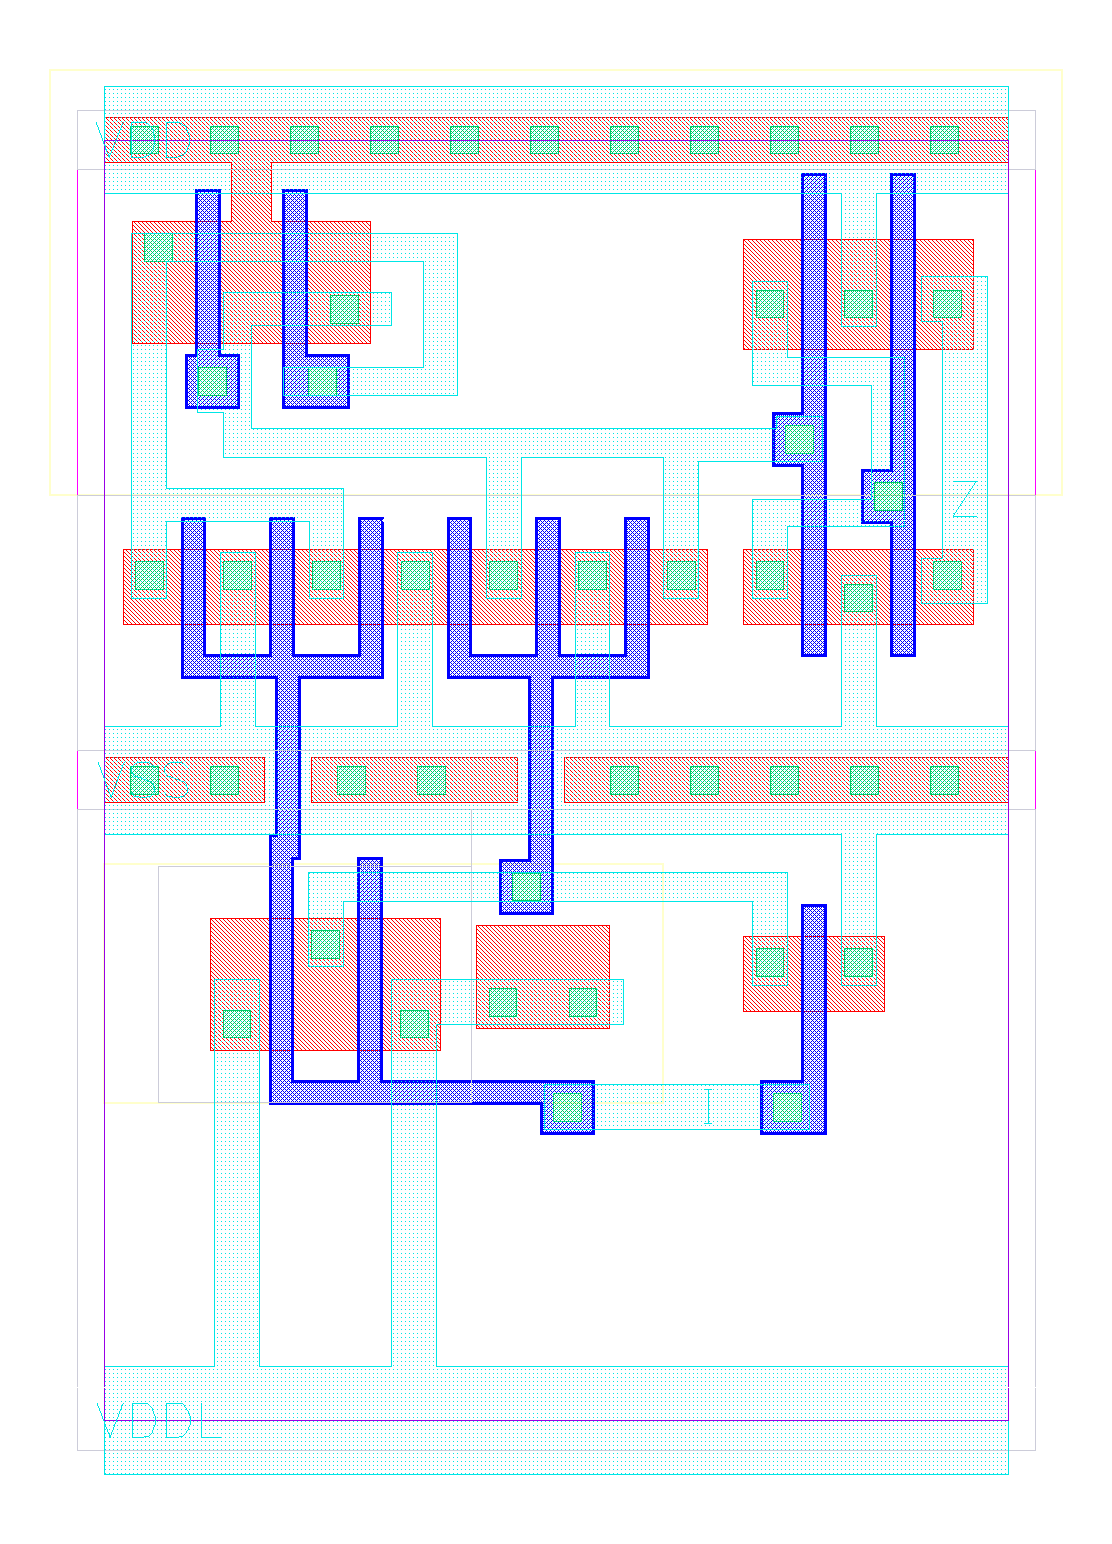
\includegraphics[scale=0.23]{slike/layout_lvl_lh.png} };
        	\draw[<->] (-3.05,-4) -- (-3.05,3.8) node[midway, left=0.2, above=0.05, rotate=90] {\footnotesize 7,38\,\textmu m\,(2$\cdot$3,69\,\textmu m)};
        	\draw[<->] (-2.75,-4.55) -- (2.75,-4.55) node[midway, right=0.1, below=0.02] {\footnotesize 5,195\,\textmu m};
        	\end{tikzpicture}
		\label{layout_lvl_lh}}
	\caption{Лејаут (а) ћелије \DCO-а, (б) претварача са високог на низак и (в) претварача са ниског на висок напонски ниво.}
	\label{layout_dco_cell_lvl_hl_lh}
\end{figure}

\subsection{Симулација рада фреквенцијски затворене петље}
Симулација рада \FLL-a у оба управљачка режима приказана је на Слици~\ref{sim_FLL}. Са приказаних графика се може видјети да се у оба управљачка режима достиже стабилно закључавање \FLL-a са излазном учестаности веома блиској траженој учестаности, при чему грешка може бити у опсегу просјечне вриједности резолуције \DCO-а (испод 3\,MHz). Међутим, иако се у оба режима исправно достиже жељена учестаност, између њих постоји разлика у брзини достизања исте. Тако, у \PID\ режиму (\P=15, \I=15, \D=0), закључавање се одвија много брже, и то за 1,83\,\textmu s, док је, поређења ради, за закључавање у режиму са двостепеним регулатором потребно 13,13\,\textmu s.
\begin{figure}[!ht]
    \centering
    \subfloat[]{
	    % FLL control simulation - PID mode
%\begin{figure}[h]%[ht]
%    \vspace{-0.6cm} % added to avoid empty space above the figure
    \begin{tikzpicture}[scale=0.9, every node/.style={scale=1}]
	        \pgfplotsset{%
                    width=14cm,
                    height=10cm
                }
       % Wave dimension setup
		\def \waveDigHeight {1.0}
		\def \waveAnaHeight {3.0}
		\def \waveSpacing   {1.0}
		\def \waveOffset    {0.2}
		% Group plot
		\begin{groupplot}
			[xlabel={\footnotesize Вријеме [\textmu s]},
			 axis line style={draw=none}, % remove axis lines and arrows
			 xtick style={draw=none}, % remove tick dash
			 ytick style={draw=none}, % remove tick dash
			 xticklabel style = {font=\footnotesize},
			 ymin=0, ymax=22, % NUM_WAVES*WAVE_HEIGHT+(NUM_WAVES+1)*WAVE_SPACING
			 xmin=0, xmax=3.0,
			 yticklabel style={xshift=0.2em} % move labels closer to axis
			]			
			% Wave position and max/min value setup
			%\def \waveDCOclkY    {2.5}
			%\def \waveFllFreqY   {\waveDCOclkY+\waveDigHeight*0.5+\waveSpacing+\waveAnaHeight*0.5}
			\def \waveFllLockY   {1.5}
			\def \waveFllFreqY   {\waveFllLockY+\waveAnaHeight*0.5+\waveSpacing+\waveDigHeight*0.5}
			\def \waveFllFreqMax {650}
			\def \waveFllFreqMin {0}
			\def \waveDCOcodeY   {\waveFllFreqY+\waveAnaHeight+\waveSpacing}
			\def \waveDCOcodeMax {255}
			\def \waveDCOcodeY   {\waveFllFreqY+\waveAnaHeight+\waveSpacing}
			\def \waveDCOcodeMax {255}
			\def \waveDCOcntY    {\waveDCOcodeY+\waveAnaHeight+\waveSpacing}
			\def \waveDCOcntMax  {25}
			\def \waveClkDivY    {\waveDCOcntY+\waveAnaHeight*0.5+\waveSpacing+\waveDigHeight*0.5}
			\def \waveRstnY      {\waveClkDivY+\waveDigHeight+\waveSpacing}
			% Draw rectangle round group plot
			\draw (0,0) rectangle (30.1em,17.6em);
			% Set up group plot
			\nextgroupplot[ylabel={}, 
			               ytick={\waveFllLockY, \waveFllLockY-0.5*\waveDigHeight+\waveOffset, \waveFllLockY+0.5*\waveDigHeight-\waveOffset, % FLL lock
			                      \waveFllFreqY, \waveFllFreqY-0.5*\waveAnaHeight+\waveOffset, \waveFllFreqY+0.5*\waveAnaHeight-\waveOffset, % FLL frequency
			                      \waveDCOcodeY, \waveDCOcodeY-0.5*\waveAnaHeight+\waveOffset, \waveDCOcodeY+0.5*\waveAnaHeight-\waveOffset, % DCO control code
			                      \waveDCOcntY,   \waveDCOcntY-0.5*\waveAnaHeight+\waveOffset,  \waveDCOcntY+0.5*\waveAnaHeight-\waveOffset, % DCO counter
			                      \waveClkDivY,   \waveClkDivY-0.5*\waveDigHeight+\waveOffset,  \waveClkDivY+0.5*\waveDigHeight-\waveOffset, % Clock
			                      \waveRstnY,       \waveRstnY-0.5*\waveDigHeight+\waveOffset,    \waveRstnY+0.5*\waveDigHeight-\waveOffset  % Reset
			                     },
			               extra y ticks={\waveFllLockY-0.5*\waveDigHeight, \waveFllLockY+0.5*\waveDigHeight, % FLL lock
                			              \waveFllFreqY-0.5*\waveAnaHeight, \waveFllFreqY+0.5*\waveAnaHeight, % FLL frequency
			                              \waveDCOcodeY-0.5*\waveAnaHeight, \waveDCOcodeY+0.5*\waveAnaHeight, % DCO control code
			                               \waveDCOcntY-0.5*\waveAnaHeight,  \waveDCOcntY+0.5*\waveAnaHeight, % DCO counter
			                               \waveClkDivY-0.5*\waveDigHeight,  \waveClkDivY+0.5*\waveDigHeight, % Clock
			                                 \waveRstnY-0.5*\waveDigHeight,    \waveRstnY+0.5*\waveDigHeight  % Reset
			                             },
			               extra tick style={grid=major, color=lightgray, dotted},        
			               extra y tick labels={},       
			               yticklabels={\textcolor{\DCOColor}{\footnotesize \framebox{FLL lock} \hspace{5pt}},
			                            \textcolor{\DCOColor}{\scriptsize 0},
			                            \textcolor{\DCOColor}{\scriptsize 1},
			                            \textcolor{\DCOColor}{\footnotesize \framebox{FLL freq} \hspace{5pt}},
			                            \textcolor{\DCOColor}{\scriptsize \waveFllFreqMin},
			                            \textcolor{\DCOColor}{\scriptsize \waveFllFreqMax},
			                            \textcolor{\PIDctrlColor}{\footnotesize \framebox{DCO code} \hspace{5pt}},
			                            \textcolor{\PIDctrlColor}{\scriptsize 0},
			                            \textcolor{\PIDctrlColor}{\scriptsize \waveDCOcodeMax},
			                            \textcolor{\CtrlPreprocColor}{\footnotesize \framebox{DCO cnt} \hspace{5pt}},
			                            \textcolor{\CtrlPreprocColor}{\scriptsize 0},
			                            \textcolor{\CtrlPreprocColor}{\scriptsize \waveDCOcntMax },
			                            \textcolor{\ClkDivColor}{\footnotesize \framebox{Clock} \hspace{5pt}},
			                            \textcolor{\ClkDivColor}{\scriptsize 0},
			                            \textcolor{\ClkDivColor}{\scriptsize 1},
			                            \textcolor{\RstnColor}{\footnotesize \framebox{Reset} \hspace{5pt}},
			                            \textcolor{\RstnColor}{\scriptsize 0},
			                            \textcolor{\RstnColor}{\scriptsize 1}                                                      
			                           }
			              ]
			% Reset signal			
			\addplot [ line width=0.4pt, \RstnColor,
			           shift={(axis direction cs:0,\waveRstnY-0.5*\waveDigHeight)}
			         ] table [x index=0, 
			                  y expr=\thisrowno{1}, 
			                  col sep=comma
			                 ] {wav/pid/fll_tb.u_fll.rst_ni.csv};
			% Clock signal
			\addplot [ line width=0.4pt, \ClkDivColor ,
			           shift={(axis direction cs:0,\waveClkDivY-0.5*\waveDigHeight)}
			         ] table [x index=0, 
			                  y expr=\thisrowno{1}, 
			                  col sep=comma
			                 ] {wav/pid/fll_tb.u_fll.clk_ref_div2.csv};
			% DCO counter sampled & synchronized			
			\addplot [ line width=0.4pt, \CtrlPreprocColor,
			           shift={(axis direction cs:0,\waveDCOcntY-0.5*\waveAnaHeight)}
			         ] table [x index=0, 
			                  y expr=\thisrowno{1}*\waveAnaHeight/\waveDCOcntMax, 
			                  col sep=comma
			                 ] {wav/pid/fll_tb.u_fll.cnt_dco_q.csv};
			% DCO code
			\addplot [ line width=0.4pt, \PIDctrlColor, 
			           shift={(axis direction cs:0,\waveDCOcodeY-0.5*\waveAnaHeight)}
			         ] table [x index=0, 
			                  y expr=\thisrowno{1}*\waveAnaHeight/\waveDCOcodeMax, 
			                  col sep=comma
			                 ] {wav/pid/fll_tb.u_fll.u_dco.code.csv};                 
            % FLL Frequency        
			\addplot [ line width=0.4pt, \DCOColor,
			           shift={(axis direction cs:0,\waveFllFreqY-0.5*\waveAnaHeight)}
			         ] table [x index=0, 
			                  y expr=\thisrowno{1}*\waveAnaHeight/\waveFllFreqMax, 
			                  col sep=comma
			                 ] {wav/pid/fll_tb.u_fll.u_dco.dco_freq_MHz.csv};    
            % FLL Lock        
			\addplot [ line width=0.4pt, \DCOColor,
			           shift={(axis direction cs:0,\waveFllLockY-0.5*\waveDigHeight)}
			         ] table [x index=0, 
			                  y expr=\thisrowno{1}, 
			                  col sep=comma
			                 ] {wav/pid/fll_tb.u_fll.lock_o.csv};               
		\end{groupplot}
		% Mark lock time
		\draw[<->]             (2.7,7.55) -- (10.4,7.55) node[midway, above=0.005] {\footnotesize Вријеме закључавања \FLL-a у \PID\ режиму: 1.825\,\textmu s};
		\draw[-, gray, dashed] (2.69,1.4) -- (2.69,7.7);
		\draw[-, gray, dashed] (10.41,0.77) -- (10.41,7.7);
    \end{tikzpicture}
%	\caption{FLL control simulation: PID mode, locking time of 1.8\,\textmu s.}
%	\label{sim_PID}    
%\end{figure}

    }
    %\hfil
    \vspace{0.2cm}
    \subfloat[]{		
	    \hspace{-0.2cm}
	    % FLL control simulation - bang-bang mode
%\begin{figure}[h]%[ht]
    \begin{tikzpicture}[scale=1, every node/.style={scale=1}]
	        \pgfplotsset{%
                    width=14cm,
                    height=10.5cm
                }
       % Wave dimension setup
		\def \waveDigHeight {1.0}
		\def \waveAnaHeight {3.0}
		\def \waveSpacing   {1.0}
		\def \waveOffset    {0.2}
		% Group plot
		\begin{groupplot}
			[xlabel={\footnotesize Вријеме [\textmu s]},
			 axis line style={draw=none}, % remove axis lines and arrows
			 xtick style={draw=none}, % remove tick dash
			 ytick style={draw=none}, % remove tick dash
			 xticklabel style = {font=\footnotesize},
			 ymin=0, ymax=22, % NUM_WAVES*WAVE_HEIGHT+(NUM_WAVES+1)*WAVE_SPACING
			 xmin=0, xmax=15.0,
			 yticklabel style={xshift=0.2em}, % move labels closer to axis
			 xtick={0,1,...,15}
			]			
			% Wave position and max/min value setup
			%\def \waveDCOclkY    {2.5}
			%\def \waveFllFreqY   {\waveDCOclkY+\waveDigHeight*0.5+\waveSpacing+\waveAnaHeight*0.5}
			\def \waveFllLockY   {1.5}
			\def \waveFllFreqY   {\waveFllLockY+\waveAnaHeight*0.5+\waveSpacing+\waveDigHeight*0.5}
			\def \waveFllFreqMax {650}
			\def \waveFllFreqMin {0}
			\def \waveDCOcodeY   {\waveFllFreqY+\waveAnaHeight+\waveSpacing}
			\def \waveDCOcodeMax {255}
			\def \waveDCOcodeY   {\waveFllFreqY+\waveAnaHeight+\waveSpacing}

			\def \waveBBupdnY  {\waveDCOcodeY+\waveAnaHeight*0.5+\waveSpacing+\waveDigHeight*0.5}
			\def \waveBBenY    {\waveBBupdnY+\waveDigHeight+\waveSpacing}

			\def \waveDCOcntY    {\waveBBenY+\waveAnaHeight*0.5+\waveSpacing+\waveDigHeight*0.5}
			\def \waveDCOcntMax  {25}
			
			\def \waveClkDivY    {\waveDCOcntY+\waveAnaHeight*0.5+\waveSpacing+\waveDigHeight*0.5}
			\def \waveRstnY      {\waveClkDivY+\waveDigHeight+\waveSpacing}
			% Draw rectangle round group plot
			\draw (0,0) rectangle (30.1em,22.5em); % [line width=0.8pt]
			% Set up group plot
			\nextgroupplot[ylabel={}, 
			               ytick={\waveFllLockY, \waveFllLockY-0.5*\waveDigHeight+\waveOffset, \waveFllLockY+0.5*\waveDigHeight-\waveOffset, % FLL frequency
			                      \waveFllFreqY, \waveFllFreqY-0.5*\waveAnaHeight+\waveOffset, \waveFllFreqY+0.5*\waveAnaHeight-\waveOffset, % FLL frequency
			                      \waveDCOcodeY, \waveDCOcodeY-0.5*\waveAnaHeight+\waveOffset, \waveDCOcodeY+0.5*\waveAnaHeight-\waveOffset, % DCO control code
			                      \waveBBupdnY,   \waveBBupdnY-0.5*\waveDigHeight+\waveOffset,  \waveBBupdnY+0.5*\waveDigHeight-\waveOffset, % Clock
   			                      \waveBBenY,   \waveBBenY-0.5*\waveDigHeight+\waveOffset,  \waveBBenY+0.5*\waveDigHeight-\waveOffset, % Clock			                      
			                      \waveDCOcntY,   \waveDCOcntY-0.5*\waveAnaHeight+\waveOffset,  \waveDCOcntY+0.5*\waveAnaHeight-\waveOffset, % DCO counter
			                      \waveClkDivY,   \waveClkDivY-0.5*\waveDigHeight+\waveOffset,  \waveClkDivY+0.5*\waveDigHeight-\waveOffset, % Clock
			                      \waveRstnY,       \waveRstnY-0.5*\waveDigHeight+\waveOffset,    \waveRstnY+0.5*\waveDigHeight-\waveOffset  % Reset
			                     },
			               extra y ticks={\waveFllLockY-0.5*\waveDigHeight, \waveFllLockY+0.5*\waveDigHeight, % FLL lock
                     		              \waveFllFreqY-0.5*\waveAnaHeight, \waveFllFreqY+0.5*\waveAnaHeight, % FLL frequency
			                              \waveDCOcodeY-0.5*\waveAnaHeight, \waveDCOcodeY+0.5*\waveAnaHeight, % DCO control code
                                          \waveBBupdnY-0.5*\waveDigHeight,  \waveBBupdnY+0.5*\waveDigHeight, % Clock
                                          \waveBBenY-0.5*\waveDigHeight,  \waveBBenY+0.5*\waveDigHeight, % Clock			                              
			                               \waveDCOcntY-0.5*\waveAnaHeight,  \waveDCOcntY+0.5*\waveAnaHeight, % DCO counter
			                               \waveClkDivY-0.5*\waveDigHeight,  \waveClkDivY+0.5*\waveDigHeight, % Clock
			                                 \waveRstnY-0.5*\waveDigHeight,    \waveRstnY+0.5*\waveDigHeight  % Reset
			                             },
			               extra tick style={grid=major, color=lightgray, dotted},        
			               extra y tick labels={},       
			               yticklabels={\textcolor{\DCOColor}{\footnotesize \framebox{FLL lock} \hspace{5pt}},
			                            \textcolor{\DCOColor}{\scriptsize 0},
			                            \textcolor{\DCOColor}{\scriptsize 1},
			                            \textcolor{\DCOColor}{\footnotesize \framebox{FLL freq} \hspace{5pt}},
			                            \textcolor{\DCOColor}{\scriptsize \waveFllFreqMin},
			                            \textcolor{\DCOColor}{\scriptsize \waveFllFreqMax},
			                            \textcolor{\BBctrlColor}{\footnotesize \framebox{DCO code} \hspace{5pt}},
			                            \textcolor{\BBctrlColor}{\scriptsize 0},
			                            \textcolor{\BBctrlColor}{\scriptsize \waveDCOcodeMax},
			                            \textcolor{\BBctrlColor}{\footnotesize \framebox{BB updn} \hspace{5pt}},
			                            \textcolor{\BBctrlColor}{\scriptsize 0},
			                            \textcolor{\BBctrlColor}{\scriptsize 1},
			                            \textcolor{\BBctrlColor}{\footnotesize \framebox{BB en} \hspace{5pt}},
			                            \textcolor{\BBctrlColor}{\scriptsize 0},
			                            \textcolor{\BBctrlColor}{\scriptsize 1},			                            			                            
			                            \textcolor{\CtrlPreprocColor}{\footnotesize \framebox{DCO cnt} \hspace{5pt}},
			                            \textcolor{\CtrlPreprocColor}{\scriptsize 0},
			                            \textcolor{\CtrlPreprocColor}{\scriptsize \waveDCOcntMax },
			                            \textcolor{\ClkDivColor}{\footnotesize \framebox{Clock} \hspace{5pt}},
			                            \textcolor{\ClkDivColor}{\scriptsize 0},
			                            \textcolor{\ClkDivColor}{\scriptsize 1},
			                            \textcolor{\RstnColor}{\footnotesize \framebox{Reset} \hspace{5pt}},
			                            \textcolor{\RstnColor}{\scriptsize 0},
			                            \textcolor{\RstnColor}{\scriptsize 1}                                                      
			                           }
			              ]
			% Reset signal			
			\addplot [ line width=0.5pt, \RstnColor,
			           shift={(axis direction cs:0,\waveRstnY-0.5*\waveDigHeight)}
			         ] table [x index=0, 
			                  y expr=\thisrowno{1}, 
			                  col sep=comma
			                 ] {wav/bb/fll_tb.u_fll.rst_ni.csv};
			% Clock signal
			\addplot [ line width=0.2pt, \ClkDivColor ,
			           shift={(axis direction cs:0,\waveClkDivY-0.5*\waveDigHeight)}
			         ] table [x index=0, 
			                  y expr=\thisrowno{1}, 
			                  col sep=comma
			                 ] {wav/bb/fll_tb.u_fll.clk_ref_div2.csv};
			% DCO counter sampled & synchronized			
			\addplot [ line width=0.5pt, \CtrlPreprocColor,
			           shift={(axis direction cs:0,\waveDCOcntY-0.5*\waveAnaHeight)}
			         ] table [x index=0, 
			                  y expr=\thisrowno{1}*\waveAnaHeight/\waveDCOcntMax, 
			                  col sep=comma
			                 ] {wav/bb/fll_tb.u_fll.cnt_dco_q.csv};
			% CNT enable signal
			\addplot [ line width=0.5pt, \BBctrlColor ,
			           shift={(axis direction cs:0,\waveBBenY-0.5*\waveDigHeight)}
			         ] table [x index=0, 
			                  y expr=\thisrowno{1}, 
			                  col sep=comma
			                 ] {wav/bb/fll_tb.u_fll.u_cnt_ref.en_i.csv};
			% CNT up down signal
			\addplot [ line width=0.5pt, \BBctrlColor ,
			           shift={(axis direction cs:0,\waveBBupdnY-0.5*\waveDigHeight)}
			         ] table [x index=0, 
			                  y expr=\thisrowno{1}, 
			                  col sep=comma
			                 ] {wav/bb/fll_tb.u_fll.u_cnt_ref.up_down_i.csv};			                 			                 
   			% DCO code
			\addplot [ line width=0.5pt, \BBctrlColor, 
			           shift={(axis direction cs:0,\waveDCOcodeY-0.5*\waveAnaHeight)}
			         ] table [x index=0, 
			                  y expr=\thisrowno{1}*\waveAnaHeight/\waveDCOcodeMax, 
			                  col sep=comma
			                 ] {wav/bb/fll_tb.u_fll.u_dco.code.csv};                 
            % FLL Frequency        
			\addplot [ line width=0.5pt, \DCOColor,
			           shift={(axis direction cs:0,\waveFllFreqY-0.5*\waveAnaHeight)}
			         ] table [x index=0, 
			                  y expr=\thisrowno{1}*\waveAnaHeight/\waveFllFreqMax, 
			                  col sep=comma
			                 ] {wav/bb/fll_tb.u_fll.u_dco.dco_freq_MHz.csv};  
            % FLL Lock        
			\addplot [ line width=0.5pt, \DCOColor,
			           shift={(axis direction cs:0,\waveFllLockY-0.5*\waveDigHeight)}
			         ] table [x index=0, 
			                  y expr=\thisrowno{1}, 
			                  col sep=comma
			                 ] {wav/bb/fll_tb.u_fll.lock_o.csv}; 			                                
		\end{groupplot}
		% Mark lock time
		\draw[<->]             (0.05,9.6) -- (11.04,9.6) node[midway, above] {\footnotesize Вријеме закључавања \FLL-а у bang-bang режиму: 13.124\,\textmu s};
		\draw[-, gray, dashed] (0.00,9.4) -- (0.00,9.8);
		\draw[-, gray, dashed] (11.09,0.8) -- (11.09,9.8);
    \end{tikzpicture}
%	\caption{FLL control simulation: bang-bang mode, locking time of 13\,\textmu s.}	
%	\label{sim_BB}    
%\end{figure}

    }	
    \caption {Симулација \FLL-а у (а) \PID\ и (б) двостепеном режиму.} % , lock time 1.8\,\textmu s lock time 13.3\,\textmu s
    \label{sim_FLL}
\end{figure}

\subsection{\PVT\ зависност дигитално контролисаног осцилатора} \label{section:impl:pvt}
Да би се одредило понашање \DCO-a у реалним условима, потребно је провјерити понашање \DCO-а при промјени процесних углова, напона напајања и температуре, односно провјерити различите \PVT\ случајеве. У оквиру овог рада симулирано је понашање у три различита \PVT\ случаја:
\begin{enumerate}
	\item Најспорији случај (slow-slow процесни угао, $V_\text{DD}$=1,1\,V, $V_\text{DDL}$=1\,V, 125\,$^{\circ}$C)
	\item Типични случај (typical-typical процесни угао, $V_\text{DD}$=1,2\,V, $V_\text{DDL}$=1,1\,V, 40\,$^{\circ}$C)
	\item Најбржи случај (fast-fast процесни угао, $V_\text{DD}$=1,3\,V, $V_\text{DDL}$=1,2\,V, -40\,$^{\circ}$C)
\end{enumerate}
\figurename~\ref{DCO_worst_typical_best} приказује зависност учестаности \DCO-a и фреквенцијског корака тј. резолуције учестаности ($K_\text{DCO}$) од броја укључених тростатичких инвертора (тј. од управљачке ријечи \DCO-a), за најспорији, типичан и најбржи \PVT\ случај. \par
\begin{figure*}[!ht]%[!b]
    \centering

    \def \SSLineStyle {solid}
    \def \TTLineStyle {dashed}
    \def \FFLineStyle {dotted}
    
    \begin{tikzpicture}[scale=1]
    \pgfplotsset{%
        width=13cm,
        height=8cm
    }
    
    \definecolor{darkgray176}{RGB}{176,176,176}
    \definecolor{darkorange25512714}{RGB}{255,127,14}
    \definecolor{forestgreen4416044}{RGB}{44,160,44}
    \definecolor{steelblue31119180}{RGB}{31,119,180}
    
    \begin{axis}[
    tick align=outside,
    tick pos=left,
    x grid style={darkgray176},
    xlabel={Број укључених тростатичких инвертора \\ \vspace{0.2cm} \scriptsize (а)},
    xmajorgrids,
    xmin=0, xmax=255,
    xtick style={color=black},
    y grid style={darkgray176},
    ylabel={Фреквенција осциловања [MHz]},
    ymajorgrids,
    ymin=0, ymax=1205.20885915,
    ytick style={color=black},
    %
    %ytick={0,0.2,...,1.2},
    xlabel style={align=center,text width=8cm},
    line width = 1pt,
    x axis line style = {line width=0.2pt},
    y axis line style = {line width=0.2pt},
    x grid style = {line width=0.2pt},
    y grid style = {line width=0.2pt},
    %legend pos=north west,
    %legend style={legend image post style={mark options={scale=0.7}}, cells={anchor=west}, at={(0.69,1)}, font=\tiny, line width=0.5pt, legend reversed=true},
    legend style={legend image post style={scale=0.82}, cells={anchor=west}, at={(0.648,1)}, font=\scriptsize, line width=0.5pt, legend reversed=true},
    tick label style={font=\footnotesize},
    label style={font=\footnotesize}
    ]
    %\addplot [steelblue31119180, mark=*, mark options={scale=0.5, mark repeat=15}]
    \addplot [steelblue31119180, solid]
    table {%
    0 27.191722
    1 28.683692
    2 30.309022
    3 32.11723
    4 34.134108
    5 36.358849
    6 37.927839
    7 39.606522
    8 41.430148
    9 43.414902
    10 45.554272
    11 47.174534
    12 48.887188
    13 50.720641
    14 52.68493
    15 54.771083
    16 56.427611
    17 58.164409
    18 60.0042
    19 61.954452
    20 64.007413
    21 65.690771
    22 67.44532
    23 69.289918
    24 71.229922
    25 73.257242
    26 74.962749
    27 76.730844
    28 78.579089
    29 80.511547
    30 82.517721
    31 84.240189
    32 86.019275
    33 87.87023
    34 89.796495
    35 91.79011
    36 93.526205
    37 95.314322
    38 97.167628
    39 99.088945
    40 101.070794
    41 102.818292
    42 104.613825
    43 106.469028
    44 108.386206
    45 110.354897
    46 112.11219
    47 113.913779
    48 115.770365
    49 117.683955
    50 119.647843
    51 121.413426
    52 123.220223
    53 125.078063
    54 126.988684
    55 128.945622
    56 130.718323
    57 132.529561
    58 134.388405
    59 136.296348
    60 138.242793
    61 140.021384
    62 141.836325
    63 143.695732
    64 145.601154
    65 147.546651
    66 149.330662
    67 151.14897
    68 153.008844
    69 154.912044
    70 156.852808
    71 158.64145
    72 160.462351
    73 162.323016
    74 164.224186
    75 166.154293
    76 167.947066
    77 169.76998
    78 171.630616
    79 173.529556
    80 175.4617
    81 177.257776
    82 179.082802
    83 180.943476
    84 182.840426
    85 184.768859
    86 186.567966
    87 188.394574
    88 190.255106
    89 192.150201
    90 194.067708
    91 195.869229
    92 197.696975
    93 199.55706
    94 201.450152
    95 203.37153
    96 205.175238
    97 207.004077
    98 208.863785
    99 210.754961
    100 212.673127
    101 214.478698
    102 216.308353
    103 218.167614
    104 220.056974
    105 221.963372
    106 223.770465
    107 225.600614
    108 227.459159
    109 229.346606
    110 231.25865
    111 233.067029
    112 234.897632
    113 236.755409
    114 238.641014
    115 240.550167
    116 242.35969
    117 244.190488
    118 246.047606
    119 247.931217
    120 249.827601
    121 251.637704
    122 253.468492
    123 255.324449
    124 257.206159
    125 259.109619
    126 260.92044
    127 262.751138
    128 264.606284
    129 266.48596
    130 268.386715
    131 270.198051
    132 272.028506
    133 273.882537
    134 275.760405
    135 277.647267
    136 279.458722
    137 281.288715
    138 283.141425
    139 285.01718
    140 286.91245
    141 288.724039
    142 290.553655
    143 292.405095
    144 294.279123
    145 296.171641
    146 297.983143
    147 299.811979
    148 301.662181
    149 303.53398
    150 305.411572
    151 307.222799
    152 309.050839
    153 310.899508
    154 312.769166
    155 314.656416
    156 316.467377
    157 318.294549
    158 320.141819
    159 322.009433
    160 323.894166
    161 325.704609
    162 327.530916
    163 329.376723
    164 331.242232
    165 333.110937
    166 334.920747
    167 336.745866
    168 338.589953
    169 340.453576
    170 342.332475
    171 344.141644
    172 345.965705
    173 347.808323
    174 349.669451
    175 351.545956
    176 353.354358
    177 355.177354
    178 357.018215
    179 358.877281
    180 360.736895
    181 362.544478
    182 364.365929
    183 366.205254
    184 368.061598
    185 369.932965
    186 371.73953
    187 373.559829
    188 375.397301
    189 377.251696
    190 379.120535
    191 380.926131
    192 382.745413
    193 384.580603
    194 386.432973
    195 388.283774
    196 390.088104
    197 391.905518
    198 393.739259
    199 395.58889
    200 397.452384
    201 399.255663
    202 401.071697
    203 402.903377
    204 404.750972
    205 406.611846
    206 408.4139
    207 410.228344
    208 412.058177
    209 413.903564
    210 415.745685
    211 417.546058
    212 419.358654
    213 421.186324
    214 423.02925
    215 424.884318
    216 426.683404
    217 428.494383
    218 430.319965
    219 432.160432
    220 434.013173
    221 435.810455
    222 437.619585
    223 439.443077
    224 441.281017
    225 443.114408
    226 444.910071
    227 446.717308
    228 448.538548
    229 450.373892
    230 452.220852
    231 454.015125
    232 455.820523
    233 457.639547
    234 459.472498
    235 461.317092
    236 463.109712
    237 464.913431
    238 466.729888
    239 468.560691
    240 470.384824
    241 472.175653
    242 473.977148
    243 475.791426
    244 477.619333
    245 479.457898
    246 481.246909
    247 483.04653
    248 484.858643
    249 486.684185
    250 488.519905
    251 490.307353
    252 492.10481
    253 493.914574
    254 495.73728
    255 497.551513
    };
    \addlegendentry{slow-slow; T=125\,\textdegree C; $\text{V}_\text{\scalebox{.8}{DD}}$=1,1\,V; $\text{V}_\text{\scalebox{.8}{DDL}}$=1,0\,V}
    %\addplot [darkorange25512714, mark=square*, mark options={scale=0.5, mark repeat=15}]
    \addplot [darkorange25512714, densely dashdotted]
    table {%
    0 41.980536
    1 44.285759
    2 46.800092
    3 49.592026
    4 52.695336
    5 56.12135
    6 58.543564
    7 61.137623
    8 63.951508
    9 67.005382
    10 70.29997
    11 72.799263
    12 75.444178
    13 78.270747
    14 81.293314
    15 84.504829
    16 87.059249
    17 89.739325
    18 92.574521
    19 95.57499
    20 98.733878
    21 101.329367
    22 104.035538
    23 106.877014
    24 109.861507
    25 112.982165
    26 115.608572
    27 118.335019
    28 121.181051
    29 124.153221
    30 127.239692
    31 129.892276
    32 132.634172
    33 135.483782
    34 138.446018
    35 141.512996
    36 144.186168
    37 146.941013
    38 149.793237
    39 152.747491
    40 155.795909
    41 158.486062
    42 161.251166
    43 164.10585
    44 167.05339
    45 170.080595
    46 172.785184
    47 175.55891
    48 178.415208
    49 181.35721
    50 184.376559
    51 187.093413
    52 189.874405
    53 192.732082
    54 195.668856
    55 198.677261
    56 201.404631
    57 204.191734
    58 207.050398
    59 209.98275
    60 212.973611
    61 215.709758
    62 218.501786
    63 221.360914
    64 224.288858
    65 227.278719
    66 230.022541
    67 232.818928
    68 235.678449
    69 238.602591
    70 241.584825
    71 244.334972
    72 247.135499
    73 249.99504
    74 252.915539
    75 255.880817
    76 258.636539
    77 261.439741
    78 264.299201
    79 267.21614
    80 270.184578
    81 272.94528
    82 275.750967
    83 278.610066
    84 281.523599
    85 284.48575
    86 287.250524
    87 290.058151
    88 292.91649
    89 295.826729
    90 298.771004
    91 301.539045
    92 304.347929
    93 307.205248
    94 310.111964
    95 313.062538
    96 315.833489
    97 318.643503
    98 321.499889
    99 324.403309
    100 327.348559
    101 330.122078
    102 332.933015
    103 335.788259
    104 338.688665
    105 341.614783
    106 344.390453
    107 347.201468
    108 350.055272
    109 352.95225
    110 355.887401
    111 358.664492
    112 361.475893
    113 364.32829
    114 367.222055
    115 370.152446
    116 372.93075
    117 375.742182
    118 378.592947
    119 381.483675
    120 384.393263
    121 387.172372
    122 389.983251
    123 392.832276
    124 395.719279
    125 398.640225
    126 401.41992
    127 404.23046
    128 407.077446
    129 409.961375
    130 412.877864
    131 415.658001
    132 418.467849
    133 421.312735
    134 424.193518
    135 427.087857
    136 429.867772
    137 432.676253
    138 435.518955
    139 438.396133
    140 441.303408
    141 444.083206
    142 446.89066
    143 449.731049
    144 452.604822
    145 455.507758
    146 458.287216
    147 461.093308
    148 463.931712
    149 466.802026
    150 469.681241
    151 472.459776
    152 475.264275
    153 478.099818
    154 480.966521
    155 483.860552
    156 486.638306
    157 489.441426
    158 492.274394
    159 495.137573
    160 498.027247
    161 500.804132
    162 503.60537
    163 506.435672
    164 509.295468
    165 512.160319
    166 514.936125
    167 517.73455
    168 520.561892
    169 523.418103
    170 526.298719
    171 529.072612
    172 531.869579
    173 534.694142
    174 537.546609
    175 540.423189
    176 543.195685
    177 545.990542
    178 548.812286
    179 551.661216
    180 554.511843
    181 557.282498
    182 560.074963
    183 562.893713
    184 565.738981
    185 568.606284
    186 571.375236
    187 574.16546
    188 576.980994
    189 579.822453
    190 582.68588
    191 585.453374
    192 588.241436
    193 591.054035
    194 593.891796
    195 596.728417
    196 599.49358
    197 602.278669
    198 605.087983
    199 607.921725
    200 610.776491
    201 613.539269
    202 616.32164
    203 619.127712
    204 621.957577
    205 624.80784
    206 627.568277
    207 630.347927
    208 633.150629
    209 635.976506
    210 638.799
    211 641.556885
    212 644.333791
    213 647.132365
    214 649.954423
    215 652.795215
    216 655.550541
    217 658.324041
    218 661.119534
    219 663.937371
    220 666.774007
    221 669.527029
    222 672.297472
    223 675.089495
    224 677.903431
    225 680.711739
    226 683.461687
    227 686.228739
    228 689.016947
    229 691.826443
    230 694.653712
    231 697.40069
    232 700.165155
    233 702.949415
    234 705.754892
    235 708.57774
    236 711.322079
    237 714.083332
    238 716.864109
    239 719.665606
    240 722.459816
    241 725.20045
    242 727.957823
    243 730.734957
    244 733.531914
    245 736.34547
    246 739.084153
    247 741.837736
    248 744.610922
    249 747.404152
    250 750.212875
    251 752.94865
    252 755.698776
    253 758.469037
    254 761.257793
    255 764.034889
    };
    \addlegendentry{typical-typical; T=40\,\textdegree C; $\text{V}_\text{\scalebox{.8}{DD}}$=1,2\,V; $\text{V}_\text{\scalebox{.8}{DDL}}$=1,1\,V}
    %\addplot [forestgreen4416044, mark=triangle*, mark options={scale=0.5, mark repeat=15}]
    \addplot [forestgreen4416044, densely dotted]
    table {%
    0 63.313495
    1 66.788901
    2 70.585845
    3 74.793272
    4 79.453051
    5 84.606318
    6 88.254323
    7 92.168267
    8 96.404905
    9 100.991931
    10 105.947313
    11 109.709158
    12 113.695569
    13 117.95091
    14 122.488761
    15 127.316862
    16 131.160345
    17 135.197792
    18 139.462686
    19 143.968235
    20 148.716378
    21 152.620132
    22 156.694628
    23 160.967364
    24 165.44824
    25 170.13638
    26 174.086846
    27 178.189442
    28 182.467808
    29 186.929688
    30 191.566407
    31 195.553605
    32 199.678269
    33 203.960897
    34 208.407192
    35 213.014824
    36 217.031303
    37 221.173949
    38 225.459663
    39 229.893587
    40 234.472199
    41 238.513549
    42 242.670741
    43 246.95951
    44 251.382187
    45 255.926819
    46 259.989449
    47 264.158373
    48 268.448044
    49 272.86203
    50 277.395509
    51 281.476093
    52 285.654704
    53 289.945542
    54 294.351554
    55 298.867619
    56 302.962694
    57 307.149958
    58 311.441839
    59 315.840301
    60 320.32811
    61 324.435658
    62 328.629453
    63 332.921046
    64 337.312747
    65 341.799429
    66 345.917811
    67 350.117438
    68 354.409103
    69 358.794712
    70 363.269311
    71 367.397052
    72 371.601592
    73 375.89287
    74 380.272742
    75 384.719806
    76 388.855292
    77 393.063438
    78 397.35354
    79 401.727508
    80 406.180123
    81 410.322195
    82 414.533148
    83 418.822113
    84 423.190498
    85 427.633254
    86 431.780908
    87 435.994264
    88 440.281661
    89 444.644551
    90 449.058138
    91 453.210305
    92 457.42483
    93 461.71013
    94 466.067435
    95 470.492098
    96 474.647761
    97 478.863685
    98 483.147282
    99 487.499367
    100 491.91537
    101 496.074905
    102 500.291537
    103 504.57285
    104 508.919895
    105 513.305017
    106 517.466698
    107 521.683415
    108 525.961982
    109 530.303604
    110 534.703516
    111 538.867163
    112 543.083676
    113 547.359675
    114 551.696126
    115 556.088463
    116 560.253775
    117 564.469654
    118 568.742748
    119 573.074311
    120 577.433564
    121 581.599359
    122 585.814131
    123 590.0841
    124 594.410014
    125 598.787658
    126 602.954124
    127 607.167549
    128 611.434419
    129 615.755129
    130 620.125374
    131 624.29217
    132 628.504192
    133 632.767583
    134 637.083032
    135 641.418209
    136 645.584348
    137 649.794217
    138 654.053718
    139 658.36366
    140 662.719574
    141 666.884693
    142 671.092552
    143 675.348506
    144 679.652889
    145 684.001814
    146 688.166334
    147 692.371792
    148 696.624298
    149 700.923444
    150 705.235618
    151 709.398835
    152 713.601019
    153 717.84871
    154 722.142057
    155 726.476719
    156 730.638301
    157 734.8378
    158 739.081234
    159 743.369016
    160 747.696876
    161 751.856516
    162 756.052999
    163 760.292206
    164 764.574271
    165 768.863854
    166 773.021161
    167 777.21374
    168 781.448189
    169 785.724592
    170 790.038295
    171 794.192813
    172 798.382413
    173 802.612457
    174 806.88311
    175 811.190109
    176 815.342262
    177 819.528502
    178 823.753895
    179 828.018954
    180 832.287061
    181 836.436748
    182 840.619427
    183 844.840563
    184 849.099891
    185 853.393825
    186 857.540302
    187 861.719453
    188 865.935533
    189 870.189143
    190 874.476095
    191 878.619243
    192 882.793829
    193 887.00459
    194 891.252458
    195 895.499169
    196 899.638499
    197 903.808463
    198 908.013939
    199 912.254896
    200 916.527221
    201 920.662595
    202 924.827835
    203 929.028026
    204 933.262673
    205 937.528024
    206 941.659994
    207 945.820768
    208 950.016329
    209 954.244358
    210 958.470636
    211 962.598237
    212 966.754458
    213 970.943687
    214 975.165451
    215 979.41695
    216 983.540895
    217 987.69229
    218 991.876346
    219 996.09146
    220 1000.335729
    221 1004.455357
    222 1008.602199
    223 1012.779977
    224 1016.989466
    225 1021.193508
    226 1025.308286
    227 1029.449503
    228 1033.622136
    229 1037.824279
    230 1042.055316
    231 1046.16571
    232 1050.303279
    233 1054.468706
    234 1058.665171
    235 1062.889064
    236 1066.994353
    237 1071.125678
    238 1075.286318
    239 1079.47656
    240 1083.660358
    241 1087.761153
    242 1091.887512
    243 1096.042119
    244 1100.226358
    245 1104.434837
    246 1108.531436
    247 1112.652882
    248 1116.802184
    249 1120.979888
    250 1125.181592
    251 1129.273701
    252 1133.389404
    253 1137.533197
    254 1141.704317
    255 1145.862237
    };
    \addlegendentry{fast-fast; T=-40\,\textdegree C; $\text{V}_\text{\scalebox{.8}{DD}}$=1,3\,V; $\text{V}_\text{\scalebox{.8}{DDL}}$=1,2\,V}
    \end{axis}
    \end{tikzpicture}
    \label{DCO_freq_worst_typical_best}
    %\hfil
    \vspace{0.3cm}
    %\hspace{0.5cm}
    \begin{tikzpicture}[scale=1]
    \hspace{0.14cm}
    \pgfplotsset{%
        width=13cm,
        height=8cm
    }
    \definecolor{darkgray176}{RGB}{176,176,176}
    \definecolor{darkorange25512714}{RGB}{255,127,14}
    \definecolor{forestgreen4416044}{RGB}{44,160,44}
    \definecolor{steelblue31119180}{RGB}{31,119,180}
    
    \begin{axis}[
    tick align=outside,
    tick pos=left,
    x grid style={darkgray176},
    xlabel={Број укључених тростатичких инвертора \\ \vspace{0.2cm} \scriptsize (б)},
    xmajorgrids,
    xmin=0, xmax=255,
    xtick style={color=black},
    y grid style={darkgray176},
    ylabel={Фреквенцијски корак ($K_\text{DCO}$) [MHz]},
    ymajorgrids,
    ymin=1.30893135, ymax=5.33578165,
    ytick style={color=black},
    %
    ytick={1,1.5,...,5},
    xlabel style={align=center,text width=8cm},
    line width = 1pt,
    x axis line style = {line width=0.2pt},
    y axis line style = {line width=0.2pt},
    x grid style = {line width=0.2pt},
    y grid style = {line width=0.2pt},
    %legend pos=north east,
    %legend style={legend image post style={mark options={scale=0.7}}, cells={anchor=west}, at={(1,1)}, font=\tiny, line width=0.5pt, legend reversed=true},
    legend style={legend image post style={scale=0.82}, cells={anchor=west}, at={(1,1)}, font=\scriptsize, line width=0.5pt, legend reversed=true},
    tick label style={font=\footnotesize},
    label style={font=\footnotesize}
    ]
    %\addplot [steelblue31119180, mark=*, mark options={scale=0.3}]
    \addplot [steelblue31119180, solid]
    table {%
    1 1.49197
    2 1.62533
    3 1.808208
    4 2.016878
    5 2.224741
    6 1.56899
    7 1.678683
    8 1.823626
    9 1.984754
    10 2.13937
    11 1.620262
    12 1.712654
    13 1.833453
    14 1.964289
    15 2.086153
    16 1.656528
    17 1.736798
    18 1.839791
    19 1.95025200000001
    20 2.052961
    21 1.683358
    22 1.754549
    23 1.844598
    24 1.940004
    25 2.02732
    26 1.705507
    27 1.768095
    28 1.84824499999999
    29 1.932458
    30 2.006174
    31 1.72246800000001
    32 1.77908599999999
    33 1.85095500000001
    34 1.92626499999999
    35 1.99361500000001
    36 1.73609500000001
    37 1.788117
    38 1.85330599999999
    39 1.921317
    40 1.98184900000001
    41 1.74749799999999
    42 1.79553300000001
    43 1.85520299999999
    44 1.91717800000001
    45 1.96869099999999
    46 1.757293
    47 1.80158900000001
    48 1.85658599999999
    49 1.91359
    50 1.963888
    51 1.76558300000001
    52 1.806797
    53 1.85784
    54 1.91062100000001
    55 1.95693799999998
    56 1.77270100000001
    57 1.811238
    58 1.858844
    59 1.90794299999999
    60 1.94644500000001
    61 1.77859100000001
    62 1.81494099999998
    63 1.859407
    64 1.90542200000002
    65 1.94549699999999
    66 1.78401099999999
    67 1.818308
    68 1.85987400000002
    69 1.9032
    70 1.940764
    71 1.78864199999998
    72 1.82090100000002
    73 1.86066499999998
    74 1.90117000000001
    75 1.93010699999999
    76 1.79277300000001
    77 1.822914
    78 1.860636
    79 1.89894000000001
    80 1.93214399999999
    81 1.796076
    82 1.82502599999998
    83 1.86067400000002
    84 1.89695
    85 1.92843299999998
    86 1.79910700000002
    87 1.82660799999999
    88 1.86053200000001
    89 1.895095
    90 1.917507
    91 1.80152099999998
    92 1.82774600000002
    93 1.860085
    94 1.893092
    95 1.921378
    96 1.803708
    97 1.82883899999999
    98 1.85970800000001
    99 1.891176
    100 1.91816599999999
    101 1.80557100000001
    102 1.829655
    103 1.85926099999998
    104 1.88936000000001
    105 1.906398
    106 1.80709300000001
    107 1.83014900000001
    108 1.85854499999999
    109 1.88744700000001
    110 1.91204399999998
    111 1.808379
    112 1.830603
    113 1.857777
    114 1.88560500000003
    115 1.90915299999998
    116 1.80952300000001
    117 1.83079799999999
    118 1.85711800000001
    119 1.883611
    120 1.89638399999998
    121 1.81010300000003
    122 1.83078799999998
    123 1.85595699999999
    124 1.88171000000003
    125 1.90346
    126 1.81082099999998
    127 1.83069800000004
    128 1.85514599999999
    129 1.87967599999996
    130 1.900755
    131 1.81133600000004
    132 1.83045499999997
    133 1.85403100000002
    134 1.87786799999998
    135 1.88686200000001
    136 1.81145500000002
    137 1.829993
    138 1.85271
    139 1.87575499999997
    140 1.89526999999998
    141 1.81158900000003
    142 1.82961599999999
    143 1.85144000000003
    144 1.87402800000001
    145 1.892518
    146 1.81150199999996
    147 1.82883600000002
    148 1.85020199999997
    149 1.87179900000001
    150 1.87759199999999
    151 1.81122700000003
    152 1.82803999999999
    153 1.84866900000003
    154 1.86965799999996
    155 1.88724999999999
    156 1.81096100000002
    157 1.82717200000002
    158 1.84726999999998
    159 1.867614
    160 1.88473299999998
    161 1.81044300000002
    162 1.82630699999999
    163 1.84580700000004
    164 1.86550899999997
    165 1.86870499999998
    166 1.80981000000003
    167 1.82511899999997
    168 1.844087
    169 1.86362300000002
    170 1.87889899999999
    171 1.809169
    172 1.82406100000003
    173 1.84261799999996
    174 1.86112800000001
    175 1.87650500000001
    176 1.808402
    177 1.82299599999999
    178 1.84086100000002
    179 1.85906599999998
    180 1.85961400000002
    181 1.80758300000002
    182 1.82145099999997
    183 1.83932500000003
    184 1.85634399999998
    185 1.87136700000002
    186 1.80656499999998
    187 1.82029899999998
    188 1.83747200000005
    189 1.85439499999995
    190 1.86883900000004
    191 1.80559599999998
    192 1.81928199999999
    193 1.83519000000001
    194 1.85237000000001
    195 1.85080099999999
    196 1.80432999999999
    197 1.81741399999999
    198 1.83374100000003
    199 1.84963099999999
    200 1.863494
    201 1.80327900000003
    202 1.81603399999995
    203 1.83168000000001
    204 1.84759500000001
    205 1.86087400000002
    206 1.802054
    207 1.81444399999998
    208 1.82983300000001
    209 1.84538700000002
    210 1.84212099999996
    211 1.80037300000004
    212 1.81259599999998
    213 1.82767000000001
    214 1.84292599999998
    215 1.85506800000002
    216 1.79908599999999
    217 1.81097900000003
    218 1.825582
    219 1.84046699999999
    220 1.85274099999998
    221 1.797282
    222 1.80912999999998
    223 1.82349200000004
    224 1.83794
    225 1.83339100000001
    226 1.79566299999999
    227 1.80723699999999
    228 1.82123999999999
    229 1.83534400000002
    230 1.84695999999997
    231 1.79427300000003
    232 1.80539799999997
    233 1.81902400000001
    234 1.83295099999998
    235 1.84459400000003
    236 1.79262
    237 1.803719
    238 1.81645700000001
    239 1.830803
    240 1.82413299999996
    241 1.79082900000003
    242 1.80149499999999
    243 1.814278
    244 1.82790699999998
    245 1.83856500000002
    246 1.78901100000002
    247 1.799621
    248 1.81211299999995
    249 1.82554200000004
    250 1.83571999999998
    251 1.78744799999998
    252 1.79745700000001
    253 1.80976400000003
    254 1.82270599999998
    255 1.814233
    };
    \addlegendentry{slow-slow; T=125\,\textdegree C; $\text{V}_\text{\scalebox{.8}{DD}}$=1,1\,V; $\text{V}_\text{\scalebox{.8}{DDL}}$=1,0\,V}
    %\addplot [darkorange25512714, mark=square*, mark options={scale=0.2}]
    \addplot [darkorange25512714, densely dashdotted]
    table {%
    1 2.305223
    2 2.514333
    3 2.791934
    4 3.10331
    5 3.426014
    6 2.422214
    7 2.59405899999999
    8 2.813885
    9 3.053874
    10 3.294588
    11 2.49929299999999
    12 2.644915
    13 2.82656900000001
    14 3.022567
    15 3.21151500000001
    16 2.55441999999999
    17 2.680076
    18 2.83519600000001
    19 3.000469
    20 3.158888
    21 2.595489
    22 2.706171
    23 2.841476
    24 2.984493
    25 3.12065799999999
    26 2.626407
    27 2.72644700000001
    28 2.84603199999999
    29 2.97217000000001
    30 3.086471
    31 2.652584
    32 2.741896
    33 2.84960999999998
    34 2.96223600000002
    35 3.06697799999998
    36 2.67317200000002
    37 2.75484499999999
    38 2.85222400000001
    39 2.95425399999999
    40 3.048418
    41 2.69015300000001
    42 2.76510400000001
    43 2.85468399999999
    44 2.94754
    45 3.02720499999998
    46 2.704589
    47 2.77372600000001
    48 2.85629800000001
    49 2.942002
    50 3.01934899999998
    51 2.71685400000001
    52 2.780992
    53 2.857677
    54 2.93677400000001
    55 3.00840499999998
    56 2.72737000000001
    57 2.787103
    58 2.858664
    59 2.93235200000001
    60 2.990861
    61 2.73614699999999
    62 2.79202800000002
    63 2.859128
    64 2.927944
    65 2.98986099999999
    66 2.74382199999999
    67 2.79638700000001
    68 2.859521
    69 2.92414199999999
    70 2.98223400000001
    71 2.750147
    72 2.80052700000002
    73 2.85954099999998
    74 2.92049900000001
    75 2.96527800000001
    76 2.75572200000002
    77 2.803202
    78 2.85945999999996
    79 2.91693900000001
    80 2.96843799999999
    81 2.76070200000004
    82 2.80568699999998
    83 2.85909900000001
    84 2.91353299999997
    85 2.96215100000001
    86 2.76477399999999
    87 2.80762700000002
    88 2.858339
    89 2.91023899999999
    90 2.944275
    91 2.76804099999998
    92 2.80888400000003
    93 2.85731899999996
    94 2.90671600000002
    95 2.95057400000002
    96 2.77095099999997
    97 2.81001400000002
    98 2.85638599999999
    99 2.90341999999998
    100 2.94525000000004
    101 2.77351899999996
    102 2.81093700000002
    103 2.85524399999997
    104 2.90040600000003
    105 2.92611799999997
    106 2.77566999999999
    107 2.811015
    108 2.85380400000003
    109 2.89697799999999
    110 2.93515100000002
    111 2.77709099999998
    112 2.81140099999999
    113 2.852397
    114 2.89376500000003
    115 2.93039099999999
    116 2.77830399999999
    117 2.81143200000002
    118 2.85076499999997
    119 2.89072800000002
    120 2.90958799999999
    121 2.77910900000001
    122 2.810879
    123 2.84902499999998
    124 2.88700299999999
    125 2.92094600000001
    126 2.779695
    127 2.81054
    128 2.84698600000002
    129 2.88392899999997
    130 2.91648900000001
    131 2.78013700000002
    132 2.80984799999999
    133 2.84488599999997
    134 2.88078300000001
    135 2.894339
    136 2.77991500000002
    137 2.80848099999997
    138 2.84270200000003
    139 2.87717800000001
    140 2.90727499999997
    141 2.77979800000003
    142 2.80745400000001
    143 2.84038899999996
    144 2.87377300000003
    145 2.90293600000001
    146 2.77945799999998
    147 2.80609199999998
    148 2.83840400000003
    149 2.87031400000001
    150 2.87921499999999
    151 2.77853499999998
    152 2.80449900000002
    153 2.83554300000003
    154 2.86670299999997
    155 2.89403099999998
    156 2.77775400000002
    157 2.80311999999998
    158 2.83296799999999
    159 2.863179
    160 2.88967400000001
    161 2.77688499999999
    162 2.80123800000001
    163 2.83030200000002
    164 2.85979600000002
    165 2.86485099999993
    166 2.77580599999999
    167 2.79842500000007
    168 2.82734199999993
    169 2.85621100000003
    170 2.88061600000003
    171 2.77389300000004
    172 2.796967
    173 2.82456300000001
    174 2.85246699999993
    175 2.87657999999999
    176 2.77249600000005
    177 2.79485699999998
    178 2.82174399999997
    179 2.84893
    180 2.85062700000003
    181 2.77065500000003
    182 2.79246499999999
    183 2.81875000000002
    184 2.84526799999992
    185 2.86730299999999
    186 2.76895200000001
    187 2.79022400000008
    188 2.81553399999996
    189 2.84145899999999
    190 2.863427
    191 2.76749400000006
    192 2.78806199999997
    193 2.81259899999998
    194 2.837761
    195 2.83662100000004
    196 2.76516299999992
    197 2.78508900000008
    198 2.80931399999997
    199 2.83374200000003
    200 2.85476599999993
    201 2.76277800000003
    202 2.78237100000001
    203 2.80607199999997
    204 2.82986500000004
    205 2.85026300000004
    206 2.76043699999991
    207 2.77965000000006
    208 2.80270199999995
    209 2.82587699999999
    210 2.82249400000001
    211 2.75788499999999
    212 2.77690600000005
    213 2.79857400000003
    214 2.82205799999997
    215 2.84079199999996
    216 2.75532599999997
    217 2.77350000000001
    218 2.79549300000008
    219 2.81783699999994
    220 2.836636
    221 2.75302199999999
    222 2.770443
    223 2.79202300000009
    224 2.8139359999999
    225 2.80830800000001
    226 2.74994800000002
    227 2.76705200000004
    228 2.78820799999994
    229 2.80949600000008
    230 2.827269
    231 2.74697800000001
    232 2.76446499999997
    233 2.78426000000002
    234 2.805477
    235 2.82284799999991
    236 2.74433900000008
    237 2.76125300000001
    238 2.78077699999994
    239 2.80149700000004
    240 2.79421000000002
    241 2.740634
    242 2.75737299999992
    243 2.77713400000005
    244 2.79695700000002
    245 2.81355599999995
    246 2.73868300000004
    247 2.75358299999994
    248 2.77318600000001
    249 2.79322999999999
    250 2.8087230000001
    251 2.73577499999999
    252 2.75012599999991
    253 2.770261
    254 2.78875600000003
    255 2.77709600000003    
    };
    \addlegendentry{typical-typical; T=40\,\textdegree C; $\text{V}_\text{\scalebox{.8}{DD}}$=1,2\,V; $\text{V}_\text{\scalebox{.8}{DDL}}$=1,1\,V}
    %\addplot [forestgreen4416044, mark=triangle*, mark options={scale=0.3}]
    \addplot [forestgreen4416044, densely dotted]
    table {%
    1 3.47540599999999
    2 3.79694400000001
    3 4.207427
    4 4.659779
    5 5.153267
    6 3.648005
    7 3.913944
    8 4.236638
    9 4.58702599999999
    10 4.955382
    11 3.76184500000001
    12 3.986411
    13 4.25534099999999
    14 4.537851
    15 4.828101
    16 3.84348300000001
    17 4.03744699999999
    18 4.264894
    19 4.505549
    20 4.748143
    21 3.90375400000002
    22 4.07449599999998
    23 4.27273600000001
    24 4.48087599999999
    25 4.68814
    26 3.95046600000001
    27 4.10259600000001
    28 4.27836599999998
    29 4.46188000000001
    30 4.636719
    31 3.98719800000001
    32 4.124664
    33 4.28262799999999
    34 4.44629500000002
    35 4.607632
    36 4.016479
    37 4.14264599999998
    38 4.28571400000001
    39 4.43392399999999
    40 4.57861199999999
    41 4.04135000000002
    42 4.15719199999998
    43 4.288769
    44 4.42267699999999
    45 4.54463200000001
    46 4.06262999999998
    47 4.168924
    48 4.289671
    49 4.41398600000002
    50 4.533479
    51 4.08058399999999
    52 4.17861099999999
    53 4.29083800000001
    54 4.40601200000003
    55 4.51606499999997
    56 4.09507500000001
    57 4.18726400000003
    58 4.29188099999999
    59 4.39846199999999
    60 4.48780899999997
    61 4.10754800000001
    62 4.19379500000002
    63 4.29159299999998
    64 4.39170100000001
    65 4.48668199999997
    66 4.118382
    67 4.19962700000002
    68 4.29166500000002
    69 4.38560899999999
    70 4.47459900000001
    71 4.12774099999996
    72 4.20454000000001
    73 4.29127800000003
    74 4.37987199999998
    75 4.44706400000001
    76 4.13548600000001
    77 4.208146
    78 4.29010199999999
    79 4.37396799999999
    80 4.45261499999998
    81 4.14207200000004
    82 4.21095299999996
    83 4.28896500000002
    84 4.36838499999999
    85 4.44275600000003
    86 4.14765399999999
    87 4.21335599999998
    88 4.287397
    89 4.36288999999999
    90 4.41358700000001
    91 4.15216700000002
    92 4.21452499999998
    93 4.28530000000001
    94 4.357305
    95 4.42466300000001
    96 4.155663
    97 4.21592399999997
    98 4.28359700000004
    99 4.35208499999999
    100 4.41600299999999
    101 4.15953500000001
    102 4.216632
    103 4.28131300000001
    104 4.34704499999998
    105 4.38512200000002
    106 4.16168099999993
    107 4.21671700000002
    108 4.27856700000007
    109 4.34162199999992
    110 4.39991200000009
    111 4.16364699999997
    112 4.21651299999996
    113 4.27599900000007
    114 4.33645100000001
    115 4.392337
    116 4.16531199999997
    117 4.21587899999997
    118 4.27309400000001
    119 4.33156299999996
    120 4.35925300000008
    121 4.165795
    122 4.21477199999993
    123 4.26996900000006
    124 4.32591400000001
    125 4.37764399999992
    126 4.16646600000001
    127 4.21342500000003
    128 4.26687000000004
    129 4.32070999999996
    130 4.37024499999995
    131 4.16679600000009
    132 4.21202199999993
    133 4.26339099999996
    134 4.31544900000006
    135 4.33517700000004
    136 4.16613899999993
    137 4.20986900000003
    138 4.259501
    139 4.30994199999998
    140 4.35591399999998
    141 4.165119
    142 4.20785899999998
    143 4.25595400000009
    144 4.30438299999992
    145 4.34892500000001
    146 4.16452000000004
    147 4.20545800000002
    148 4.25250599999993
    149 4.29914600000006
    150 4.31217400000003
    151 4.16321699999992
    152 4.20218399999999
    153 4.24769100000003
    154 4.29334700000004
    155 4.33466199999998
    156 4.16158199999995
    157 4.19949900000006
    158 4.24343399999998
    159 4.28778199999999
    160 4.32785999999999
    161 4.15964000000008
    162 4.19648299999994
    163 4.23920699999996
    164 4.28206499999999
    165 4.28958299999999
    166 4.15730700000006
    167 4.19257900000002
    168 4.23444899999993
    169 4.27640300000007
    170 4.31370299999992
    171 4.15451800000005
    172 4.18960000000004
    173 4.23004399999991
    174 4.27065300000004
    175 4.30699900000002
    176 4.152153
    177 4.18624
    178 4.22539300000005
    179 4.26505899999995
    180 4.26810699999999
    181 4.14968699999997
    182 4.18267900000001
    183 4.221136
    184 4.25932799999998
    185 4.29393400000004
    186 4.146477
    187 4.17915100000005
    188 4.21607999999992
    189 4.25360999999998
    190 4.28695200000004
    191 4.143148
    192 4.17458599999998
    193 4.21076100000005
    194 4.24786800000004
    195 4.246711
    196 4.13932999999997
    197 4.16996399999994
    198 4.20547600000009
    199 4.24095699999998
    200 4.27232500000002
    201 4.13537399999996
    202 4.16524000000004
    203 4.2001909999999
    204 4.234647
    205 4.26535100000001
    206 4.13197000000002
    207 4.16077400000006
    208 4.195561
    209 4.22802899999999
    210 4.22627799999998
    211 4.12760100000003
    212 4.15622099999996
    213 4.18922899999995
    214 4.22176400000001
    215 4.25149900000008
    216 4.12394499999994
    217 4.15139499999998
    218 4.18405600000006
    219 4.21511399999997
    220 4.24426900000003
    221 4.11962800000003
    222 4.14684199999999
    223 4.17777799999999
    224 4.20948899999996
    225 4.20404199999996
    226 4.114778
    227 4.1412170000001
    228 4.17263299999991
    229 4.20214299999998
    230 4.23103700000001
    231 4.11039400000004
    232 4.13756899999998
    233 4.16542700000014
    234 4.19646499999999
    235 4.22389299999986
    236 4.10528900000008
    237 4.13132500000006
    238 4.16063999999983
    239 4.19024200000013
    240 4.18379800000002
    241 4.10079499999983
    242 4.12635900000009
    243 4.15460699999994
    244 4.18423899999993
    245 4.20847900000012
    246 4.09659899999997
    247 4.12144600000011
    248 4.14930199999981
    249 4.17770400000018
    250 4.20170399999984
    251 4.09210900000016
    252 4.11570299999994
    253 4.14379299999996
    254 4.17111999999997
    255 4.1579200000001   
    };
    \addlegendentry{fast-fast; T=-40\,\textdegree C; $\text{V}_\text{\scalebox{.8}{DD}}$=1,3\,V; $\text{V}_\text{\scalebox{.8}{DDL}}$=1,2\,V}
    \end{axis}
    \end{tikzpicture}
    \label{DCO_kdco_worst_typical_best}
    
    \caption{Зависност (а) фреквенције осциловања и (б) фреквенцијског корака од броја укључених тростатичких инвертора за најспорији, типични и најбржи случај.}
    \label{DCO_worst_typical_best}
\end{figure*}

\tablename~\ref{tab:frequency_ranges_and_average_kdco} приказује фреквенцијски опсег \DCO-а и просјечну вриједност фреквенцијског корака ($K_\text{DCO}$) у три претходно обрађена случаја. Под опсегом се подразумијевају минималне и максималне вриједности учестаности која се добија на излазу \DCO-а за укључен мининалан (у овом случају 15) и максималан број (у овом случају 255) тростатичких инвертора \DCO-а, респективно.
\begin{table}[!ht]
	\caption{Фреквенцијски опсег \DCO-a и просјечна вриједност фреквенцијског корака ($K_\text{DCO}$).}
	\label{tab:frequency_ranges_and_average_kdco}
	\centering
	\begin{tabular}{|c|c|c|c|}
		\hline
		Случај & $f_{\min}$ & $f_{\max}$ & Просјечан $K_\text{DCO}$ \\
		\specialrule{1pt}{0pt}{0pt}
		Најспорији & 27,2\,MHz & 502\,MHz & 1,8\,MHz \\
		\hline
		Типичнни& 42\,MHz & 764\,MHz & 2,8\,MHz \\
		\hline
		Најбржи & 63,3\,MHz & 1,146\,GHz & 4,2\,MHz \\
		\hline
	\end{tabular}
\end{table}
Иако у најспоријем случају учестаност не достиже жељених 640\,МHz, oна ипак може бити достигнута повећањем засебног напона напајања осцилатора ($V_\text{DDL}$). Такође је могуће анализирати и зависност учестаности од свих \PVT\ параметара независно, међутим те зависности нису приказане у раду због временске захтјевности извршавања потребних симулација, као и због већ приказаних резултата симулација у најспоријем, типичном и најбржем случају, који су ипак најбитнији за анализу понашања имплементираног система јер се ослањају на понашање система у граничним условима рада. Ипак, што се тиче понашања \DCO-а у зависности од свих \PVT\ параметара појединачно, потребно је напоменути да се учестаност повећава са бржим процесним углом, већим напоном напајања, као и мањом температуром. \par
Да би се значајно смањило вријеме потребно за добијање резултата из симулација након екстракције лејаута, и то са минималним губитком прецизности добијених резултата, симулације \DCO-a су извршене на нивоу појединачно екстракованих ћелија \DCO-a и екстракованих претварача напонског нивоа, са додатним паразитним кондензатором на свакој фази \DCO-a. Улога тих кондензатора је да надомјесте паразитне капацитивности које се јављају у потпуно екстракованом лејауту \DCO-a због међусобно повезаних ћелија, а које нису аутоматски урачунате ако се симулације врше на нивоу појединачно екстракованих компоненти \DCO-a, као што је то овде случај. Вриједност капацитивности додатог кондензатора прорачуната је на основу извјештаја генерисаног из екстракције паразитних капацитивности на нивоу читавог дизајна.  

\subsection{Анализа потрошње система} \label{section:impl:dco_pwr}
Потрошња снаге сваког дизајна утиче на велики број критичних одлука при самом пројектовању, као што су одређивање капацитивности извора напајања, трајања батерије, величине линија напајања, начина паковања, захтјева за хлађењем система итд. Значи да је потрошња снаге важна особина дизајна јер значајно утиче на изводљивост примјене крајњег производа, као и на трошкове и поузданост при коришћењу~\cite{RABAEY:2003digital}. \par
Зависно од проблема који се анализира, разматрају се различите мјере потрошње снаге. Рецимо, када се разматра величина линија напајања, тада је битна максимална вриједност снаге \engl{Peak Power}, $P_{peak}$, док при разматрању захтјева за хлађењем или складиштењем енергије тј. батеријом, од главног интереса је просјечна потрошња снаге \engl{Average Power Dissipation}~\cite{RABAEY:2003digital}. Те мјере су дефинисане следећим формулама:
\begin{equation}
	\label{eq:impl:dco_pwr:peak}
	P_{peak} = i_{peak}V_{supply} = \max [p(t)]
\end{equation}
\begin{equation}
	\label{eq:impl:dco_pwr:av}
	P_{avg} = \frac{1}{T}\int_{0}^{T}p(t)dt = \frac{V_{supply}}{T}\int_{0}^{T}i_{supply}(t)dt
\end{equation}
гдје је $i_{supply}$ струја која долази од извора са напоном $V_{supply}$ у интервалу $t \in [0,T]$, док је $i_{peak}$ максимална вриједност $i_{supply}$ унутар тог интервала. \par
Од горе поменутих, у овом раду је кључна просјечна потрошња снаге. Како је \DCO\ кључни елемент \FLL-a, он је и убједљиво највећи потрошач у систему. Самим тим, његовим изолованим симулацијама се може умногоме предвидјети и потрошња коначног система, што значи да се пројектовање убрзава тиме што није потребно баш увијек радити симулације дизајна читавог \FLL-a како би се приближно одредила потрошња. \par
Све симулације потрошње које слиједе су извршаване за учестаност осциловања од 640\,MHz. Након симулације дизајна \DCO-a (са претварачима напонских нивоа) у типичним условима рада, при чему су $V_\text{DD}$=1,2\,V и $V_\text{DDL}$=1,1\,V, добија се вриједност просјечне потрошње од 2,5\,mW од извора напајања $V_\text{DDL}$ одакле се напајају осцилатор, претварачи са високог на низак и једним дијелом претварачи са ниског на висок напонски ниво и 0,22\,mW од извора напајања $V_\text{DD}$ одакле се, у овој симулацији, већим дијелом напајају претварачи са ниског на висок напонски ниво као и излазни бафери (погледати поглавље~\ref{LS chapter}). \par
Потрошња се може утврдити и преко средње квадратне \engl[RMS]{Root Mean Square} вриједности струје која се добија при истим условима и овде износи 2,185\,mA и 0,18\,mA од извора напајања $V_\text{DDL}$ и $V_\text{DD}$, респективно. С обзиром да је средња квадратна вриједност струје величина директно сразмјерна просјечној потрошњи снаге, при анализи потрошње углавном је довољно навести резултате у једној од тих величина. Формула за RMS вриједност потрошње струје неког извора гласи:
%Множењем RMS вриједности струје са напоном напајања добија се приближно поменута вриједност просјечног расипања снаге, па је углавном довољно навести један од та два параметра потрошње.\begin{equation}
\begin{equation}
	\label{eq:impl:dco_pwr:rms_i}
	\text{rms}(i_{supply}) = \sqrt{\frac{1}{T}\int_{0}^{T}i_{supply}^{2}(t)dt}
\end{equation}
% TODO
% Провјерити тврдње изнад
Резултати симулације наведени у претходним параграфу, од читавог \FLL-a, обухватају \DCO\ са претварачима напонских нивоа. Да би се утврдила и потрошња управљачке логике (која се напаја са извора $V_\text{DD}$), под истим условима је покренута и симулација потрошње читавог \FLL-a, гдје се на изворима напајања $V_\text{DDL}$ и $V_\text{DD}$ добијају RMS вриједности потрошње струје 2,185\,mA и 0,9\,mA, респективно. Ако се од укупне RMS вриједности струје са $V_\text{DD}$ извора напајања од 0,9\,mA одузме изнад поменута вриједност коју троше само претварачи са ниског на висок напонски ниво и излазни бафери \DCO-а (0,18\,mA), добије се RMS вриједност потрошње струје управљачке логике \FLL-a и износи 0,72\,mA.

\subsection{Временски одзив дигитално контролисаног осцилатора}
Временски одзив \engl{Timing} односи се на облик сигнала на фазама дигитално контролисаног осцилатора на нивоу једне периоде излазног такта. У сврху приказа временског одзива симулиран је рад екстракованог \DCO-а у типичним условима. \par
\begin{figure}[!ht]
    \centering
    \begin{tikzpicture}[scale=1]
    \pgfplotsset{%
        width=11cm,
        height=9cm
    }

    \definecolor{crimson2143940}{RGB}{214,39,40}
    \definecolor{darkgray176}{RGB}{176,176,176}

    \definecolor{colorPHL}{RGB}{0,0,255}

    \definecolor{colorPH}{RGB}{255,0,0}

    \def \PHZeroLineStyle {solid}
    \def \PHOneLineStyle {dashed}
    \def \PHTwoLineStyle {dotted}
    \def \PHThreeLineStyle {loosely dashdotted}
    \def \PHFourLineStyle {densely dashdotdotted}
    
    \begin{axis}[
    tick align=outside,
    tick pos=left,
    x grid style={darkgray176},
    xlabel={Вријеме [ns]},
    xmajorgrids,
    xmin=0, xmax=1.565,
    xtick style={color=black},
    y grid style={darkgray176},
    ylabel={Напон [V]},
    ymajorgrids,
    ymin=-0.105097200727831, ymax=1.34749448635499,
    ytick style={color=black},
    %
    ytick={0,0.1,...,1.2},
    xtick={0,0.3,...,1.5},
    xlabel style={align=center,text width=6cm},
    line width = 1pt,
    x axis line style = {line width=0.2pt},
    y axis line style = {line width=0.2pt},
    x grid style = {line width=0.2pt},
    y grid style = {line width=0.2pt},
    legend style={at={(1.21,0.75)}, font=\scriptsize, line width=0.5pt},
    tick label style={font=\footnotesize},
    label style={font=\footnotesize}
    ]
    \addplot [colorPHL, \PHZeroLineStyle]
    table {%
    0 1.09993165775137
    0.00251739135936904 1.09984968227474
    0.00712501830602127 1.09963477423175
    0.0124367573782921 1.09930460438077
    0.0158757884526497 1.09905477964008
    0.0186486421614145 1.09877188578219
    0.0222036416072085 1.0984133566538
    0.0267939103824663 1.09803270151327
    0.0310038512400835 1.09775385145054
    0.0354144573274245 1.09751613475672
    0.0404449476903705 1.09742231382188
    0.0457247901171645 1.09819175392966
    0.0514907993088071 1.1011059818364
    0.0539530466889192 1.10340041632519
    0.0568296444715165 1.10701932047766
    0.0606541922165963 1.1142165081197
    0.0655007717633147 1.12668149508568
    0.0696978797384338 1.13963382567739
    0.0733507925472146 1.15190472338815
    0.0764168707523716 1.16197513088554
    0.079892698109474 1.17022832244604
    0.0823989275691689 1.17163644712062
    0.0846284840726037 1.16805819512424
    0.08837038426132 1.1481680096407
    0.0911340703885772 1.11557085905248
    0.0932068293203161 1.07238895533593
    0.0954176490116616 1.01169802837402
    0.0985767350772809 0.906042916742654
    0.101492557451299 0.792771763395389
    0.103790409478373 0.695511049786902
    0.106132576302695 0.591435393606577
    0.109113403312555 0.455804498500798
    0.111714624623314 0.339989380348085
    0.114123910196651 0.243086553866559
    0.116904613454125 0.155814409192333
    0.120152886833132 0.0888013071636188
    0.12327278180897 0.0505564058549625
    0.126634546306798 0.0276236573278167
    0.130518452788465 0.0143196838727978
    0.133806954914661 0.00871704762372326
    0.138731822398915 0.00460816468260774
    0.144050563878403 0.00260901831908277
    0.146639141860345 0.00204636452096016
    0.149869665159164 0.00153480407558726
    0.15437959747441 0.00104441738241922
    0.158327696320317 0.000751555547570526
    0.161749306813043 0.000567422874475353
    0.165668872446222 0.000409800933320233
    0.169322893082406 0.000298126319273538
    0.172615914365896 0.000222773015625057
    0.175462923277514 0.000175139763267231
    0.179057065150121 0.000133133524839255
    0.182784067706652 0.000103722816093482
    0.186057101210724 8.51022049655613e-05
    0.189703145511623 6.93439011594335e-05
    0.193768370187538 5.6014185866145e-05
    0.197391664838053 4.68161476547594e-05
    0.199159030215897 4.30883795647639e-05
    0.20040981815446 4.06781308777231e-05
    0.202868874922946 3.63495225716187e-05
    0.206248418058552 3.1287714695278e-05
    0.209744277275479 2.6972183531743e-05
    0.213047667108897 2.35334176669154e-05
    0.215823660097123 2.10090262126162e-05
    0.217956611696855 1.9260203823342e-05
    0.220110018020288 1.7640352659371e-05
    0.223113483511858 1.5571396831984e-05
    0.225862206059711 1.38393681558079e-05
    0.228744661118598 1.21903537968565e-05
    0.231958703346875 1.05673865450357e-05
    0.235840012523341 8.9038654847053e-06
    0.239369315887512 7.63604445262123e-06
    0.24236800809853 6.70852532275047e-06
    0.246058002276698 5.72016545624823e-06
    0.249684036981516 4.88662553965435e-06
    0.252828475874955 4.25933571050596e-06
    0.256132123544131 3.68486879143704e-06
    0.260872088601979 2.99363155151837e-06
    0.264712988623759 2.53354869989122e-06
    0.268823893580915 2.12523722005165e-06
    0.272622272395298 1.81362597878415e-06
    0.27582046957353 1.59279041992759e-06
    0.278427879907095 1.43700507604262e-06
    0.281611152797491 1.27240962784958e-06
    0.2848591001325 1.12958701331724e-06
    0.288217297624027 1.00470852726582e-06
    0.292496616849262 8.73623463756761e-07
    0.296420350452516 7.76277224616624e-07
    0.300777816075285 6.8892834488861e-07
    0.305960967044311 6.07704117296161e-07
    0.311991287970116 5.3702741209737e-07
    0.316412566404526 4.97716614813273e-07
    0.321945875302672 4.5976025948138e-07
    0.326717350772469 4.34835841303055e-07
    0.329778607798648 4.21858461476296e-07
    0.332652442730187 4.11443892116322e-07
    0.336696426097225 3.99218067116436e-07
    0.341089136913778 3.88584257687023e-07
    0.345332706077944 3.80513381829438e-07
    0.349839676648721 3.73498109573421e-07
    0.35487434607039 3.67419299577888e-07
    0.360615307819541 3.62310635907394e-07
    0.365453141160382 3.59213448957744e-07
    0.367910596232333 3.57932869891891e-07
    0.370707267201268 3.56674595943671e-07
    0.375163905529139 3.55003888395385e-07
    0.379921354116767 3.53529968105981e-07
    0.383661502846919 3.52539959826663e-07
    0.387310116788957 3.51719920332316e-07
    0.390420299070923 3.51142039673424e-07
    0.393753038462993 3.50636269188976e-07
    0.396010438320997 3.50348641817687e-07
    0.398912949371303 3.50029409836168e-07
    0.402534986616616 3.49694300898074e-07
    0.404868698089278 3.49510130078916e-07
    0.406883569449633 3.49369031843482e-07
    0.409477169132029 3.49210287285555e-07
    0.412685909970646 3.49047173364917e-07
    0.415378236580189 3.48936602247392e-07
    0.417613116565924 3.48861560973502e-07
    0.420301650055971 3.48789589936681e-07
    0.423033057287985 3.4873515277881e-07
    0.425678555601795 3.48699183125115e-07
    0.428013163898278 3.48680216241552e-07
    0.431152290156987 3.48666264510584e-07
    0.434255160339301 3.48667948657016e-07
    0.43742862402292 3.48699490380718e-07
    0.440912503681679 3.48737533058094e-07
    0.444755038487807 3.48755620590048e-07
    0.448412322851105 3.48725907416742e-07
    0.453853122413342 3.48590753718992e-07
    0.458179708246437 3.48443378408254e-07
    0.460821962102478 3.48353732932846e-07
    0.464178895514725 3.48245847089178e-07
    0.46900982166197 3.48105351117625e-07
    0.47226784443944 3.4803483082947e-07
    0.476019226846349 3.48509496963682e-07
    0.480078851065539 3.4810344994446e-07
    0.483746155354655 3.47971483411001e-07
    0.486626982578782 3.48126779400452e-07
    0.48964110275818 3.48464652599691e-07
    0.49348556675608 3.48884714422308e-07
    0.497093373272346 3.48842094947893e-07
    0.500370977273703 3.48310197202322e-07
    0.504198459282724 3.47550934423479e-07
    0.508251923834177 3.46722618574045e-07
    0.511280238269832 3.4638372994338e-07
    0.512897590098059 3.46343922552726e-07
    0.514348938832187 3.4638256265162e-07
    0.5175409885664 3.46636916765588e-07
    0.520996154265989 3.47076714409067e-07
    0.524433867565073 3.47427013369265e-07
    0.527550902447939 3.47747067162242e-07
    0.53001123543098 3.47995251349924e-07
    0.532023316006842 3.48189357721309e-07
    0.534790381802586 3.48637664675286e-07
    0.537544322008907 3.48792254837977e-07
    0.540343612163811 3.48867287926944e-07
    0.543356374714923 3.48939251190965e-07
    0.546846968955031 3.49011489385128e-07
    0.550838230781317 3.49041251279688e-07
    0.553987364260747 3.4901156606442e-07
    0.556954413273445 3.48930873870842e-07
    0.561144858693918 3.48733165083454e-07
    0.564482943953599 3.48510409896501e-07
    0.567132119944144 3.48297001856754e-07
    0.571506070344314 3.47885088728094e-07
    0.575926104299601 3.47392960715757e-07
    0.579857596884914 3.46874780858355e-07
    0.583847292905278 3.4626309707618e-07
    0.587430387030227 3.45625929953087e-07
    0.59021564292001 3.45063996461101e-07
    0.592886392846411 3.43926035154882e-07
    0.596489623397933 3.43136666829787e-07
    0.599522419778172 3.42683532470284e-07
    0.603311078414259 3.41880050032854e-07
    0.607903499701747 3.4070622026918e-07
    0.611323272917799 3.3988164199315e-07
    0.616041210596664 3.39179704166026e-07
    0.622232166637313 3.49383262723355e-07
    0.62695110729556 3.41804665690994e-07
    0.632159659531944 3.33190028485158e-07
    0.637670628326237 3.3103139689956e-07
    0.641474228592101 3.28432953621456e-07
    0.644197998490421 3.2472004600948e-07
    0.647489019446539 3.18830030832666e-07
    0.652060958880072 3.13854561503355e-07
    0.656275445184438 3.22097651119521e-07
    0.660640959001775 3.38382949401153e-07
    0.665549390447208 3.43041439325063e-07
    0.670512797975376 3.36830553107688e-07
    0.67654975968761 3.47484352928525e-07
    0.679624792816495 3.67069602357474e-07
    0.682276832787681 4.00238309116298e-07
    0.685551680167526 4.85957341799117e-07
    0.690612256012755 7.75233400095197e-07
    0.695113401229449 1.15185720248763e-06
    0.698745823591363 1.50070201233963e-06
    0.701876046953202 1.864138798854e-06
    0.705158661884161 2.42203048363287e-06
    0.708308227137511 2.88980072336939e-06
    0.710213552586847 3.24442014753001e-06
    0.713725830264174 4.54795740787338e-06
    0.716928410414319 5.42029032997248e-06
    0.71909120248723 5.55045764780835e-06
    0.721158508211709 5.37666597113971e-06
    0.724185940588256 4.68466920416579e-06
    0.727204193783869 3.64451443805224e-06
    0.729577017852174 2.68828800688128e-06
    0.731852727707434 1.6658181250148e-06
    0.734872957206912 -5.32615960441314e-08
    0.737440796387242 -2.47030586099245e-06
    0.739935481323714 -6.54366566513405e-06
    0.742459644238342 -1.33997958189305e-05
    0.745800464159346 -2.50485358376035e-05
    0.748890618802196 -3.85882675981595e-05
    0.752187258480762 -5.47000638072984e-05
    0.755936473980225 -7.21314740391688e-05
    0.759435750506611 -9.75885475219904e-05
    0.764025063154403 -0.000107075952467129
    0.769908302745487 -9.59639261909557e-05
    0.772477100445758 -8.96029915081519e-05
    0.775415765035144 -7.45354381224093e-05
    0.779608589839365 -1.65766732751172e-06
    0.784017728938003 0.000138809608924799
    0.787276924606542 0.000309780635988835
    0.791214315858089 0.000695209415279229
    0.794924812705114 0.00113213665445615
    0.798425232464306 0.00148793944635126
    0.801163408644597 0.00169636507183784
    0.80463905173003 0.00185719448388477
    0.808419416444941 0.00191458463778245
    0.811766185093778 0.00188570779569594
    0.815324370474802 0.00177713894222772
    0.819367543569937 0.00148605822305284
    0.823166349515176 0.00090466163007185
    0.825210797922781 0.000440808999750152
    0.82659242209905 7.1839986936454e-05
    0.828959316028804 -0.000688789769355608
    0.832333644736354 -0.00195634410378235
    0.835829956053158 -0.00351134064434125
    0.839141333638059 -0.00532210088068162
    0.841966042050055 -0.00752206317126857
    0.844118870428396 -0.00983924906122994
    0.846266590157023 -0.0122182104791151
    0.849269155186097 -0.0155370202828816
    0.85201664495797 -0.0186234370736494
    0.854897724042096 -0.021986430932762
    0.858108554991142 -0.0259447996355066
    0.861983753775251 -0.0307902885192634
    0.865539801782076 -0.0339026177984289
    0.868538425797948 -0.0338465809624855
    0.872226843147808 -0.0280833489218068
    0.875856083677387 -0.0126868608950025
    0.879000506694504 0.0128582888528397
    0.882302103254432 0.0614456395574961
    0.887040329496484 0.171235181459639
    0.890882368965851 0.290273871267817
    0.894992940454381 0.439464757252457
    0.898791846042776 0.588310579707574
    0.901991342848104 0.712715992280513
    0.904598880344733 0.803536703414154
    0.907781327352357 0.88892394050287
    0.911030200673385 0.94779715226919
    0.91438741065427 0.989611066178454
    0.918665466991603 1.02601582989642
    0.922594773908524 1.04861292011416
    0.926950999065835 1.06564863521528
    0.932133709843783 1.07871981795395
    0.938164566716265 1.08780828908308
    0.942583163494498 1.09187192165034
    0.948116531733211 1.09510107043402
    0.952889368347844 1.09682523416725
    0.955952585658495 1.09759158666779
    0.958826164423256 1.09814023287439
    0.962869643618258 1.09870700132055
    0.9672626004973 1.0991261462282
    0.971506371116327 1.09939685278107
    0.976013144745896 1.09958808151887
    0.981047872348749 1.09972616783908
    0.986788342277788 1.09982399014335
    0.991626783811864 1.09987636749923
    0.994084224485571 1.09989609931769
    0.996880869193487 1.09991416414793
    1.00133653472495 1.09993560501091
    1.00609396158935 1.09995179389014
    1.00983476778238 1.09996134612639
    1.01348328165202 1.09996867541493
    1.01659334195751 1.09997363464831
    1.01992224675326 1.09997792952801
    1.02218130150324 1.09998035715619
    1.02507907913016 1.09998300990859
    1.02870152095419 1.09998572612991
    1.03103791002953 1.0999871779537
    1.03304878264017 1.09998825805606
    1.0356324829829 1.09998943845468
    1.03884284220468 1.09999062773733
    1.04153936849788 1.09999142886255
    1.0437746555781 1.09999197746116
    1.04646074483232 1.09999253413562
    1.04919640387959 1.09999302810766
    1.05184192042932 1.09999345431051
    1.05417686093182 1.0999937900414
    1.05731158920666 1.09999418134778
    1.06041615593357 1.09999450604391
    1.06358872624653 1.09999478154535
    1.06707060277375 1.09999503000879
    1.07091175288877 1.09999525266818
    1.07455204316428 1.09999542525203
    1.07998334660232 1.09999563135386
    1.08435893482773 1.0999957641338
    1.08699678095889 1.09999583033297
    1.09035281878673 1.09999590324872
    1.09518346568391 1.09999598991267
    1.09844198681824 1.09999603804452
    1.10219315768977 1.09999608466796
    1.10625245428808 1.09999612595265
    1.10991912086135 1.09999615621677
    1.11280022571984 1.09999617596882
    1.11581408163903 1.09999619334526
    1.11965858884827 1.09999621131526
    1.12326658541836 1.09999622456572
    1.12654416990774 1.09999623403953
    1.13037144250205 1.09999624254562
    1.13442508598798 1.09999624922786
    1.13745419988891 1.09999625337435
    1.1390723801905 1.0999962550806
    1.14052477106393 1.0999962563915
    1.1437169688845 1.09999625868365
    1.14717218263081 1.09999626050815
    1.15060982843757 1.09999626165966
    1.1537267021838 1.09999626234097
    1.15618657600028 1.09999626270611
    1.15819861887804 1.09999626291554
    1.1609660592615 1.0999962632839
    1.1637198301426 1.09999626324295
    1.16651914898904 1.0999962630978
    1.16953198593441 1.09999626292831
    1.17302273116191 1.09999626274616
    1.17701373878587 1.09999626254927
    1.18016239881497 1.09999626234275
    1.18312947699672 1.09999626210314
    1.18731985722704 1.09999626173782
    1.19065795676938 1.09999626144308
    1.19330717063995 1.09999626121385
    1.19768118075324 1.09999626085328
    1.20210117866109 1.0999962605188
    1.20603270185556 1.09999626024994
    1.21002238025137 1.09999626000478
    1.21360544878599 1.09999625980875
    1.21639067601561 1.09999625967135
    1.21906144236636 1.09999625955106
    1.22266466025583 1.09999625940592
    1.22569746850442 1.09999625929796
    1.22948616317855 1.0999962591814
    1.23407853232839 1.09999625906973
    1.23749823713952 1.09999625900943
    1.24221618619316 1.09999625896423
    1.24840714643183 1.09999625887893
    1.25312605870675 1.09999625897386
    1.25833470587933 1.09999625917328
    1.26384564806025 1.09999625923603
    1.26764921336879 1.09999625922676
    1.27037295464268 1.09999625920727
    1.2736639907828 1.09999625917351
    1.27823593359742 1.09999625910363
    1.28245041847671 1.09999625904073
    1.28681593027006 1.09999625946525
    1.29172437530595 1.09999625830433
    1.29668779350318 1.09999625778196
    1.30272474558334 1.09999625792194
    1.30579972393814 1.09999625825105
    1.30845180028001 1.09999625871276
    1.31172668125431 1.09999625937861
    1.31678725582839 1.0999962600764
    1.32128838387778 1.09999626002995
    1.32492083023739 1.09999625964538
    1.32805104186786 1.09999625927338
    1.33133365909881 1.09999625897722
    1.33448336338703 1.09999625879925
    1.336388699025 1.09999625872553
    1.33990110944775 1.0999962586172
    1.34310352844872 1.09999625853333
    1.34526644184581 1.09999625848688
    1.3473338884897 1.09999625845596
    1.35036146166795 1.09999625844762
    1.35337962187644 1.09999625850122
    1.3557523538894 1.0999962586008
    1.35802811543548 1.0999962587548
    1.36104825001567 1.09999625906552
    1.36361612612515 1.09999625944955
    1.36611074191878 1.09999625995718
    1.36863505839622 1.09999626058157
    1.37197581099682 1.09999626176565
    1.37506598523185 1.09999626331272
    1.37836266587444 1.09999626548506
    1.38211196717026 1.09999626858202
    1.38561152640379 1.09999627191079
    1.39020117106975 1.09999627894374
    1.39608452468381 1.09999628507437
    1.39865205398457 1.09999628574656
    1.40159062329557 1.09999628627813
    1.40578342091669 1.09999628120376
    1.41019259240096 1.09999628843596
    1.41345176033888 1.09999629853442
    1.41738913250942 1.09999631476872
    1.42109963090614 1.09999633670566
    1.42460003875773 1.09999635968472
    1.42733819830099 1.09999637031327
    1.43081381339333 1.09999636569418
    1.43459419547836 1.0999963411864
    1.43794098812005 1.09999630744441
    1.44149915315431 1.09999625916374
    1.44554232098123 1.09999619502968
    1.44934115440179 1.0999961390879
    1.45138565656896 1.09999611426511
    1.45276737449793 1.09999609971517
    1.45513434819687 1.09999607755064
    1.45850868213738 1.09999604435785
    1.46200499211415 1.09999598301387
    1.46531635999894 1.09999586794893
    1.46814104869109 1.0999956909227
    1.47029384278042 1.09999551216437
    1.47244157715749 1.09999528277196
    1.47544414267627 1.09999488487146
    1.47819163528446 1.09999443580609
    1.48107271739781 1.09999400072158
    1.48428355617804 1.09999361329632
    1.48815877020704 1.09999326495737
    1.49171475378254 1.09999265185125
    1.49471337799113 1.09999073178379
    1.49840179900025 1.09998951906269
    1.50203103203953 1.0999899594537
    1.50517545508505 1.09999083167095
    1.50847705637725 1.09999173400306
    1.513215286634 1.09999312843397
    1.51705732345152 1.09999692676024
    1.52116789571114 1.10000619705363
    1.52496680008322 1.10001950606639
    1.52816629388626 1.10003565467226
    1.53077383108701 1.10005591039034
    1.53395628011665 1.10009051669809
    1.53720515129772 1.10012258778556
    1.54056236358973 1.10014482786349
    1.54484042288385 1.10015186868755
    1.54876971659679 1.10013818510157
    1.55312594451138 1.10010790557345
    1.55830865620643 1.1000584629341
    1.56433951187494 1.09995950997656
    };
    \addlegendentry{PH0\_L}
    \addplot [colorPHL, \PHOneLineStyle]
    table {%
    0 3.43699775434292e-07
    0.00251739135936904 3.38094435596272e-07
    0.00712501830602127 3.3264299482467e-07
    0.0124367573782921 3.30548824722602e-07
    0.0158757884526497 3.27633781016315e-07
    0.0186486421614145 3.2355184352315e-07
    0.0222036416072085 3.17198494828521e-07
    0.0267939103824663 3.14315367575302e-07
    0.0310038512400835 3.25488447487793e-07
    0.0354144573274245 3.40805123323391e-07
    0.0404449476903705 3.41834794467422e-07
    0.0457247901171645 3.36755590127406e-07
    0.0514907993088071 3.53028485078401e-07
    0.0539530466889192 3.71868254634495e-07
    0.0568296444715165 4.13875880321062e-07
    0.0606541922165963 5.39591329967621e-07
    0.0655007717633147 8.56079149362341e-07
    0.0696978797384338 1.22190044998219e-06
    0.0733507925472146 1.58187170835999e-06
    0.0764168707523716 2.01121358971425e-06
    0.079892698109474 2.55689703731722e-06
    0.0823989275691689 2.91100276172604e-06
    0.0846284840726037 3.42107621975049e-06
    0.08837038426132 4.84615689024272e-06
    0.0911340703885772 5.46796047525545e-06
    0.0932068293203161 5.54264461104918e-06
    0.0954176490116616 5.30660935432622e-06
    0.0985767350772809 4.51038413651607e-06
    0.101492557451299 3.46556467242013e-06
    0.103790409478373 2.52245484583003e-06
    0.106132576302695 1.44243695991906e-06
    0.109113403312555 -3.69737900345175e-07
    0.111714624623314 -3.04307594176078e-06
    0.114123910196651 -7.34694610505102e-06
    0.116904613454125 -1.55264750027253e-05
    0.120152886833132 -2.71974881649506e-05
    0.12327278180897 -4.15519820396725e-05
    0.126634546306798 -5.74776651100447e-05
    0.130518452788465 -7.63217321807597e-05
    0.133806954914661 -0.000100498186256365
    0.138731822398915 -0.000106222648965244
    0.144050563878403 -9.52056105578219e-05
    0.146639141860345 -8.85916812356157e-05
    0.149869665159164 -6.80998183702006e-05
    0.15437959747441 2.2081627251527e-05
    0.158327696320317 0.000159832453401384
    0.161749306813043 0.000356573991360308
    0.165668872446222 0.000769787666297029
    0.169322893082406 0.0011958923201657
    0.172615914365896 0.00151981122229677
    0.175462923277514 0.00172517613004531
    0.179057065150121 0.0018736014485153
    0.182784067706652 0.00191449941716115
    0.186057101210724 0.00187642162622494
    0.189703145511623 0.00175073891739627
    0.193768370187538 0.00142063788358099
    0.197391664838053 0.000822031815778476
    0.199159030215897 0.000409650654095659
    0.20040981815446 7.40066052355068e-05
    0.202868874922946 -0.000717945415001355
    0.206248418058552 -0.00199292319964591
    0.209744277275479 -0.00355490955415639
    0.213047667108897 -0.00537285908828968
    0.215823660097123 -0.00755473777393666
    0.217956611696855 -0.00985329636121452
    0.220110018020288 -0.012238428307925
    0.223113483511858 -0.0155583273341156
    0.225862206059711 -0.0186467122862225
    0.228744661118598 -0.0220124934655647
    0.231958703346875 -0.0259763885537685
    0.235840012523341 -0.030826457497544
    0.239369315887512 -0.0339049456064974
    0.24236800809853 -0.0338442372213831
    0.246058002276698 -0.0280672892289899
    0.249684036981516 -0.0126705046793525
    0.252828475874955 0.0128884569669505
    0.256132123544131 0.0615339103214458
    0.260872088601979 0.171417333789553
    0.264712988623759 0.290457656371316
    0.268823893580915 0.439684864429064
    0.272622272395298 0.588517663500129
    0.27582046957353 0.712862864278214
    0.278427879907095 0.803657082946115
    0.281611152797491 0.889025793315948
    0.2848591001325 0.947852088462203
    0.288217297624027 0.989659884665004
    0.292496616849262 1.02605678613262
    0.296420350452516 1.0486146376826
    0.300777816075285 1.06565373219523
    0.305960967044311 1.07872384084769
    0.311991287970116 1.08780998288097
    0.316412566404526 1.0918750545202
    0.321945875302672 1.09510292945205
    0.326717350772469 1.09682603735837
    0.329778607798648 1.09759176768025
    0.332652442730187 1.09814041523245
    0.336696426097225 1.09870718637907
    0.341089136913778 1.09912625035976
    0.345332706077944 1.09939691226694
    0.349839676648721 1.09958812736053
    0.35487434607039 1.09972619564894
    0.360615307819541 1.09982401353826
    0.365453141160382 1.09987637788376
    0.367910596232333 1.09989610791692
    0.370707267201268 1.09991417109843
    0.375163905529139 1.09993561381132
    0.379921354116767 1.09995180024124
    0.383661502846919 1.09996134964183
    0.387310116788957 1.09996867834191
    0.390420299070923 1.09997363719838
    0.393753038462993 1.09997793602599
    0.396010438320997 1.09998036111892
    0.398912949371303 1.09998301718455
    0.402534986616616 1.0999857316805
    0.404868698089278 1.0999871811847
    0.406883569449633 1.09998826286954
    0.409477169132029 1.09998944656487
    0.412685909970646 1.09999063361488
    0.415378236580189 1.09999143252465
    0.417613116565924 1.09999198045906
    0.420301650055971 1.09999253715627
    0.423033057287985 1.09999303006298
    0.425678555601795 1.09999345605286
    0.428013163898278 1.09999379155113
    0.431152290156987 1.09999418312242
    0.434255160339301 1.09999450736183
    0.43742862402292 1.09999478270658
    0.440912503681679 1.09999503108568
    0.444755038487807 1.09999525361122
    0.448412322851105 1.09999542676583
    0.453853122413342 1.09999563288367
    0.458179708246437 1.09999576401456
    0.460821962102478 1.09999583033247
    0.464178895514725 1.09999590326693
    0.46900982166197 1.09999598993198
    0.47226784443944 1.0999960380543
    0.476019226846349 1.09999608467846
    0.480078851065539 1.09999612596412
    0.483746155354655 1.09999615623087
    0.486626982578782 1.09999617597901
    0.48964110275818 1.09999619335515
    0.49348556675608 1.09999621132283
    0.497093373272346 1.09999622457106
    0.500370977273703 1.09999623404376
    0.504198459282724 1.0999962425492
    0.508251923834177 1.09999624923057
    0.511280238269832 1.09999625337535
    0.512897590098059 1.09999625508064
    0.514348938832187 1.09999625639067
    0.5175409885664 1.09999625868296
    0.520996154265989 1.09999626050767
    0.524433867565073 1.09999626165936
    0.527550902447939 1.09999626234081
    0.53001123543098 1.09999626270606
    0.532023316006842 1.09999626291551
    0.534790381802586 1.09999626328387
    0.537544322008907 1.09999626324298
    0.540343612163811 1.09999626309784
    0.543356374714923 1.09999626292835
    0.546846968955031 1.09999626274621
    0.550838230781317 1.09999626254931
    0.553987364260747 1.09999626234276
    0.556954413273445 1.09999626210316
    0.561144858693918 1.09999626173783
    0.564482943953599 1.09999626144309
    0.567132119944144 1.09999626121386
    0.571506070344314 1.0999962608533
    0.575926104299601 1.09999626051881
    0.579857596884914 1.09999626024996
    0.583847292905278 1.0999962600048
    0.587430387030227 1.09999625980876
    0.59021564292001 1.09999625967136
    0.592886392846411 1.09999625955106
    0.596489623397933 1.09999625940593
    0.599522419778172 1.09999625929796
    0.603311078414259 1.0999962591814
    0.607903499701747 1.09999625906973
    0.611323272917799 1.09999625900943
    0.616041210596664 1.09999625896423
    0.622232166637313 1.09999625887893
    0.62695110729556 1.09999625897386
    0.632159659531944 1.09999625917328
    0.637670628326237 1.09999625923603
    0.641474228592101 1.09999625922676
    0.644197998490421 1.09999625920727
    0.647489019446539 1.09999625917351
    0.652060958880072 1.09999625910363
    0.656275445184438 1.09999625904073
    0.660640959001775 1.09999625946525
    0.665549390447208 1.09999625830434
    0.670512797975376 1.09999625778197
    0.67654975968761 1.09999625792194
    0.679624792816495 1.09999625825105
    0.682276832787681 1.09999625871275
    0.685551680167526 1.0999962593786
    0.690612256012755 1.0999962600764
    0.695113401229449 1.09999626002995
    0.698745823591363 1.09999625964539
    0.701876046953202 1.09999625927339
    0.705158661884161 1.09999625897723
    0.708308227137511 1.09999625879926
    0.710213552586847 1.09999625872554
    0.713725830264174 1.09999625861721
    0.716928410414319 1.09999625853333
    0.71909120248723 1.09999625848689
    0.721158508211709 1.09999625845596
    0.724185940588256 1.09999625844761
    0.727204193783869 1.0999962585012
    0.729577017852174 1.09999625860077
    0.731852727707434 1.09999625875477
    0.734872957206912 1.09999625906548
    0.737440796387242 1.09999625944948
    0.739935481323714 1.09999625995711
    0.742459644238342 1.09999626058143
    0.745800464159346 1.09999626176547
    0.748890618802196 1.09999626331248
    0.752187258480762 1.09999626548471
    0.755936473980225 1.09999626858153
    0.759435750506611 1.09999627190997
    0.764025063154403 1.09999627894183
    0.769908302745487 1.09999628507391
    0.772477100445758 1.09999628574654
    0.775415765035144 1.09999628627811
    0.779608589839365 1.09999628120367
    0.784017728938003 1.09999628843616
    0.787276924606542 1.09999629853479
    0.791214315858089 1.09999631476935
    0.794924812705114 1.0999963367065
    0.798425232464306 1.09999635968549
    0.801163408644597 1.09999637031353
    0.80463905173003 1.09999636569343
    0.808419416444941 1.09999634118501
    0.811766185093778 1.09999630744276
    0.815324370474802 1.09999625916132
    0.819367543569937 1.09999619502704
    0.823166349515176 1.09999613908609
    0.825210797922781 1.09999611426418
    0.82659242209905 1.09999609971528
    0.828959316028804 1.09999607755145
    0.832333644736354 1.09999604435906
    0.835829956053158 1.09999598301612
    0.839141333638059 1.09999586795291
    0.841966042050055 1.09999569092772
    0.844118870428396 1.09999551216708
    0.846266590157023 1.09999528277725
    0.849269155186097 1.09999488487779
    0.85201664495797 1.09999443581385
    0.854897724042096 1.09999400072846
    0.858108554991142 1.09999361330243
    0.861983753775251 1.09999326496334
    0.865539801782076 1.09999265185617
    0.868538425797948 1.09999073178985
    0.872226843147808 1.09998951906364
    0.875856083677387 1.09998995945247
    0.879000506694504 1.09999083166942
    0.882302103254432 1.09999173400052
    0.887040329496484 1.09999312842712
    0.890882368965851 1.09999692674223
    0.894992940454381 1.10000619701771
    0.898791846042776 1.10001950601992
    0.901991342848104 1.10003565462309
    0.904598880344733 1.1000559103087
    0.907781327352357 1.10009051659077
    0.911030200673385 1.10012258772012
    0.91438741065427 1.10014482781787
    0.918665466991603 1.10015186870328
    0.922594773908524 1.10013818510074
    0.926950999065835 1.1001079055942
    0.932133709843783 1.10005846297315
    0.938164566716265 1.09995951002801
    0.942583163494498 1.09981847657202
    0.948116531733211 1.09953381770164
    0.952889368347844 1.09922184598105
    0.955952585658495 1.09897831679388
    0.958826164423256 1.09867432660335
    0.962869643618258 1.09828702036942
    0.9672626004973 1.09794663509286
    0.971506371116327 1.09768138195305
    0.976013144745896 1.09745925247857
    0.981047872348749 1.09749826669622
    0.986788342277788 1.09879999713477
    0.991626783811864 1.10184738420517
    0.994084224485571 1.10437635441482
    0.996880869193487 1.10825347123466
    1.00133653472495 1.1175396672797
    1.00609396158935 1.13061056422624
    1.00983476778238 1.1425207602909
    1.01348328165202 1.1548582982654
    1.01659334195751 1.16463896574343
    1.01992224675326 1.17117049858721
    1.02218130150324 1.17125425937906
    1.02507907913016 1.1638432287094
    1.02870152095419 1.13813822122978
    1.03103791002953 1.10405243023805
    1.03304878264017 1.05763264424164
    1.0356324829829 0.981958701679159
    1.03884284220468 0.868496079230985
    1.04153936849788 0.760189567922426
    1.0437746555781 0.663804004603814
    1.04646074483232 0.543031103201631
    1.04919640387959 0.418594830335446
    1.05184192042932 0.303462317575291
    1.05417686093182 0.215188555050082
    1.05731158920666 0.128321129018352
    1.06041615593357 0.0742066725395995
    1.06358872624653 0.0417509451950717
    1.06707060277375 0.0225035320507911
    1.07091175288877 0.0119843811280703
    1.07455204316428 0.00710111081262718
    1.07998334660232 0.00367818292066283
    1.08435893482773 0.00235964047130292
    1.08699678095889 0.00185253815527943
    1.09035281878673 0.00138071365648817
    1.09518346568391 0.000917695360191602
    1.09844198681824 0.000700488914579841
    1.10219315768977 0.000514874518945321
    1.10625245428808 0.000365821519442058
    1.10991912086135 0.000264776037595695
    1.11280022571984 0.000205656807760217
    1.11581408163903 0.000160550265678859
    1.11965858884827 0.000121243234007722
    1.12326658541836 9.61498285869437e-05
    1.12654416990774 7.93050580103339e-05
    1.13037144250205 6.42976933250827e-05
    1.13442508598798 5.22097077458201e-05
    1.13745419988891 4.50617663159356e-05
    1.1390723801905 4.18112491132729e-05
    1.14052477106393 3.91101695203719e-05
    1.1437169688845 3.38476531989897e-05
    1.14717218263081 2.91326542253241e-05
    1.15060982843757 2.52349955114313e-05
    1.1537267021838 2.22059799855602e-05
    1.15618657600028 2.00855881961119e-05
    1.15819861887804 1.85053030390559e-05
    1.1609660592615 1.65169544698921e-05
    1.1637198301426 1.47046383642602e-05
    1.16651914898904 1.30183411035884e-05
    1.16953198593441 1.13907320704588e-05
    1.17302273116191 9.75612644279354e-06
    1.17701373878587 8.19067880323905e-06
    1.18016239881497 7.14670749067963e-06
    1.18312947699672 6.28796027930459e-06
    1.18731985722704 5.2446489582951e-06
    1.19065795676938 4.53462162259728e-06
    1.19330717063995 4.03802825769162e-06
    1.19768118075324 3.33286186084284e-06
    1.20210117866109 2.74760794294971e-06
    1.20603270185556 2.3190577821744e-06
    1.21002238025137 1.95908377371335e-06
    1.21360544878599 1.6903759025032e-06
    1.21639067601561 1.51203823818401e-06
    1.21906144236636 1.36280593970235e-06
    1.22266466025583 1.19068845570311e-06
    1.22569746850442 1.06827502234622e-06
    1.22948616317855 9.39631074441369e-07
    1.23407853232839 8.13674198896333e-07
    1.23749823713952 7.37468316119797e-07
    1.24221618619316 6.52136442599724e-07
    1.24840714643183 5.67612205992647e-07
    1.25312605870675 5.19251842727419e-07
    1.25833470587933 4.7808417174307e-07
    1.26384564806025 4.45204074457853e-07
    1.26764921336879 4.27493410221394e-07
    1.27037295464268 4.16830518527033e-07
    1.2736639907828 4.05831342629972e-07
    1.27823593359742 3.93394828096234e-07
    1.28245041847671 3.84319329291695e-07
    1.28681593027006 3.76897113963603e-07
    1.29172437530595 3.70102903044757e-07
    1.29668779350318 3.64900020776301e-07
    1.30272474558334 3.60387742554341e-07
    1.30579972393814 3.58625837045347e-07
    1.30845180028001 3.57332812769485e-07
    1.31172668125431 3.55973926705245e-07
    1.31678725582839 3.54240069810321e-07
    1.32128838387778 3.52954779728339e-07
    1.32492083023739 3.52071986890242e-07
    1.32805104186786 3.51431300914037e-07
    1.33133365909881 3.50877952719568e-07
    1.33448336338703 3.50444702558029e-07
    1.336388699025 3.50219829696673e-07
    1.33990110944775 3.4986166038356e-07
    1.34310352844872 3.49588274372931e-07
    1.34526644184581 3.49428567138123e-07
    1.3473338884897 3.49293140843866e-07
    1.35036146166795 3.49123341176502e-07
    1.35337962187644 3.4898548215876e-07
    1.3557523538894 3.48897410958219e-07
    1.35802811543548 3.48828326893527e-07
    1.36104825001567 3.48757716361508e-07
    1.36361612612515 3.48715122393536e-07
    1.36611074191878 3.4868832782302e-07
    1.36863505839622 3.48674045864719e-07
    1.37197581099682 3.48660670908798e-07
    1.37506598523185 3.48681624368196e-07
    1.37836266587444 3.4871871762492e-07
    1.38211196717026 3.48751546832729e-07
    1.38561152640379 3.48749344671279e-07
    1.39020117106975 3.48674410962357e-07
    1.39608452468381 3.48490939601135e-07
    1.39865205398457 3.48401782075873e-07
    1.40159062329557 3.48304548176768e-07
    1.40578342091669 3.48174424954315e-07
    1.41019259240096 3.48060090378058e-07
    1.41345176033888 3.4833818810082e-07
    1.41738913250942 3.48315871644971e-07
    1.42109963090614 3.47987717450902e-07
    1.42460003875773 3.48032591038426e-07
    1.42733819830099 3.48264498757418e-07
    1.43081381339333 3.48723381210806e-07
    1.43459419547836 3.48927425698206e-07
    1.43794098812005 3.48659686549876e-07
    1.44149915315431 3.47949822465621e-07
    1.44554232098123 3.47099573695947e-07
    1.44934115440179 3.4647749213107e-07
    1.45138565656896 3.46351045748668e-07
    1.45276737449793 3.46352431696475e-07
    1.45513434819687 3.46481128243739e-07
    1.45850868213738 3.46879109707874e-07
    1.46200499211415 3.4725520724113e-07
    1.46531635999894 3.47593231587413e-07
    1.46814104869109 3.47882118149203e-07
    1.47029384278042 3.48094917600364e-07
    1.47244157715749 3.48389175446367e-07
    1.47544414267627 3.48735747580354e-07
    1.47819163528446 3.48832390138734e-07
    1.48107271739781 3.48902404709874e-07
    1.48428355617804 3.48976795126234e-07
    1.48815877020704 3.49033395612079e-07
    1.49171475378254 3.49032954710816e-07
    1.49471337799113 3.48978280336844e-07
    1.49840179900025 3.48839358188388e-07
    1.50203103203953 3.48631619042278e-07
    1.50517545508505 3.48399153101085e-07
    1.50847705637725 3.48109447046266e-07
    1.513215286634 3.4762349017475e-07
    1.51705732345152 3.47156665537914e-07
    1.52116789571114 3.46572552589433e-07
    1.52496680008322 3.4594416388008e-07
    1.52816629388626 3.45336414764455e-07
    1.53077383108701 3.44781467916129e-07
    1.53395628011665 3.43418974595706e-07
    1.53720515129772 3.42935481367144e-07
    1.54056236358973 3.42339265105158e-07
    1.54484042288385 3.41307349287281e-07
    1.54876971659679 3.40301680400169e-07
    1.55312594451138 3.39425745977067e-07
    1.55830865620643 3.3910821534366e-07
    1.56433951187494 3.46780958774169e-07
    };
    \addlegendentry{PH1\_L}
    \addplot [colorPHL, \PHTwoLineStyle]
    table {%
    0 1.09999625893773
    0.00251739135936904 1.09999625906533
    0.00712501830602127 1.09999625919364
    0.0124367573782921 1.09999625922759
    0.0158757884526497 1.09999625921669
    0.0186486421614145 1.09999625919782
    0.0222036416072085 1.09999625916153
    0.0267939103824663 1.09999625908675
    0.0310038512400835 1.09999625903354
    0.0354144573274245 1.09999625924218
    0.0404449476903705 1.09999625813052
    0.0457247901171645 1.09999625776041
    0.0514907993088071 1.09999625801664
    0.0539530466889192 1.09999625832816
    0.0568296444715165 1.09999625885904
    0.0606541922165963 1.09999625961177
    0.0655007717633147 1.09999626012467
    0.0696978797384338 1.09999625996599
    0.0733507925472146 1.09999625954876
    0.0764168707523716 1.09999625919798
    0.079892698109474 1.09999625891612
    0.0823989275691689 1.0999962587876
    0.0846284840726037 1.09999625870558
    0.08837038426132 1.0999962585944
    0.0911340703885772 1.09999625852432
    0.0932068293203161 1.09999625848154
    0.0954176490116616 1.09999625845169
    0.0985767350772809 1.09999625845229
    0.101492557451299 1.09999625851625
    0.103790409478373 1.09999625862273
    0.106132576302695 1.09999625879332
    0.109113403312555 1.09999625911942
    0.111714624623314 1.09999625953016
    0.114123910196651 1.09999626004416
    0.116904613454125 1.09999626076496
    0.120152886833132 1.09999626199708
    0.12327278180897 1.09999626364101
    0.126634546306798 1.09999626595526
    0.130518452788465 1.09999626927273
    0.133806954914661 1.09999627245239
    0.138731822398915 1.09999628050027
    0.144050563878403 1.09999628517417
    0.146639141860345 1.09999628581459
    0.149869665159164 1.09999628637142
    0.15437959747441 1.09999628163412
    0.158327696320317 1.09999628978202
    0.161749306813043 1.09999630080856
    0.165668872446222 1.09999631797731
    0.169322893082406 1.09999634058439
    0.172615914365896 1.09999636169132
    0.175462923277514 1.09999637091619
    0.179057065150121 1.09999636297364
    0.182784067706652 1.09999633647938
    0.186057101210724 1.09999630184642
    0.189703145511623 1.09999625069225
    0.193768370187538 1.09999618594119
    0.197391664838053 1.09999613390006
    0.199159030215897 1.09999611290016
    0.20040981815446 1.09999609979324
    0.202868874922946 1.09999607679092
    0.206248418058552 1.09999604320427
    0.209744277275479 1.09999598085351
    0.213047667108897 1.09999586404448
    0.215823660097123 1.09999568834645
    0.217956611696855 1.0999955109805
    0.220110018020288 1.09999528055359
    0.223113483511858 1.09999488212829
    0.225862206059711 1.09999443245968
    0.228744661118598 1.09999399776039
    0.231958703346875 1.09999361069615
    0.235840012523341 1.09999326244967
    0.239369315887512 1.09999264952843
    0.24236800809853 1.09999072890698
    0.246058002276698 1.09998951865642
    0.249684036981516 1.09998996011039
    0.252828475874955 1.0999908324808
    0.256132123544131 1.0999917352285
    0.260872088601979 1.09999313163512
    0.264712988623759 1.09999693532061
    0.268823893580915 1.10000621403009
    0.272622272395298 1.10001952822432
    0.27582046957353 1.10003567892531
    0.278427879907095 1.1000559508702
    0.281611152797491 1.10009056792463
    0.2848591001325 1.10012261982326
    0.288217297624027 1.10014484948784
    0.292496616849262 1.10015186131265
    0.296420350452516 1.10013818238731
    0.300777816075285 1.1001078916442
    0.305960967044311 1.10005843866063
    0.311991287970116 1.09995947288624
    0.316412566404526 1.0998183035559
    0.321945875302672 1.09953356540434
    0.326717350772469 1.09922164533187
    0.329778607798648 1.09897822980996
    0.332652442730187 1.09867420709889
    0.336696426097225 1.09828687761766
    0.341089136913778 1.09794653833212
    0.345332706077944 1.09768131381795
    0.349839676648721 1.09745919973143
    0.35487434607039 1.09749837731127
    0.360615307819541 1.09880072423356
    0.365453141160382 1.10184847302533
    0.367910596232333 1.10437780982413
    0.370707267201268 1.10825555990778
    0.375163905529139 1.11754512750423
    0.379921354116767 1.13061737810172
    0.383661502846919 1.14252607721045
    0.387310116788957 1.1548640239003
    0.390420299070923 1.16464399694441
    0.393753038462993 1.17117571134612
    0.396010438320997 1.17125007748986
    0.398912949371303 1.16380552635847
    0.402534986616616 1.13804953134285
    0.404868698089278 1.1039433537122
    0.406883569449633 1.05737982678137
    0.409477169132029 0.981328389819658
    0.412685909970646 0.867810983573499
    0.415378236580189 0.759613452946431
    0.417613116565924 0.663215721866379
    0.420301650055971 0.542313122198342
    0.423033057287985 0.418075834200057
    0.425678555601795 0.302987957758187
    0.428013163898278 0.214811912431496
    0.431152290156987 0.127978624176636
    0.434255160339301 0.0740215060106551
    0.43742862402292 0.0416395214338968
    0.440912503681679 0.022438557658112
    0.444755038487807 0.011950809388326
    0.448412322851105 0.00706750368412479
    0.453853122413342 0.00366026158611611
    0.458179708246437 0.00236055514504259
    0.460821962102478 0.00185251107914596
    0.464178895514725 0.00138059197770738
    0.46900982166197 0.00091759716308233
    0.47226784443944 0.000700444202856156
    0.476019226846349 0.000514832904000766
    0.480078851065539 0.000365780137070641
    0.483746155354655 0.000264730334304014
    0.486626982578782 0.000205627372887717
    0.48964110275818 0.00016052589444279
    0.49348556675608 0.000121227550379617
    0.497093373272346 9.61397771967614e-05
    0.500370977273703 7.92972541262845e-05
    0.504198459282724 6.42910798328082e-05
    0.508251923834177 5.22051342190056e-05
    0.511280238269832 4.50597361472194e-05
    0.512897590098059 4.18110067233996e-05
    0.514348938832187 3.91118174194345e-05
    0.5175409885664 3.38492629471343e-05
    0.520996154265989 2.91340414461557e-05
    0.524433867565073 2.52360972919834e-05
    0.527550902447939 2.22067974308199e-05
    0.53001123543098 2.00859519692086e-05
    0.532023316006842 1.85056115631384e-05
    0.534790381802586 1.65174945909369e-05
    0.537544322008907 1.47050299751559e-05
    0.540343612163811 1.30187149680218e-05
    0.543356374714923 1.13911013281536e-05
    0.546846968955031 9.75650632325761e-06
    0.550838230781317 8.19090294010188e-06
    0.553987364260747 7.14675576356843e-06
    0.556954413273445 6.2880110397705e-06
    0.561144858693918 5.24467711117499e-06
    0.564482943953599 4.53464918576498e-06
    0.567132119944144 4.03805973264168e-06
    0.571506070344314 3.3328967276633e-06
    0.575926104299601 2.74763222741241e-06
    0.579857596884914 2.31908105430469e-06
    0.583847292905278 1.95910156958042e-06
    0.587430387030227 1.69038910005589e-06
    0.59021564292001 1.51204803604437e-06
    0.592886392846411 1.36281538316468e-06
    0.596489623397933 1.1906957930301e-06
    0.599522419778172 1.06828176566634e-06
    0.603311078414259 9.39637751543289e-07
    0.607903499701747 8.13678212049397e-07
    0.611323272917799 7.3747028733758e-07
    0.616041210596664 6.52138171933387e-07
    0.622232166637313 5.67613511104171e-07
    0.62695110729556 5.19252607110778e-07
    0.632159659531944 4.78085407976133e-07
    0.637670628326237 4.45204863447011e-07
    0.641474228592101 4.27493908880811e-07
    0.644197998490421 4.16830846411976e-07
    0.647489019446539 4.05831665197018e-07
    0.652060958880072 3.93395089257695e-07
    0.656275445184438 3.84319535327584e-07
    0.660640959001775 3.76897275312743e-07
    0.665549390447208 3.70103043332209e-07
    0.670512797975376 3.64900138311657e-07
    0.67654975968761 3.60387819609088e-07
    0.679624792816495 3.58625874019642e-07
    0.682276832787681 3.57332861461314e-07
    0.685551680167526 3.55973980649807e-07
    0.690612256012755 3.54240111240263e-07
    0.695113401229449 3.52954808965874e-07
    0.698745823591363 3.52072017221505e-07
    0.701876046953202 3.51431324640179e-07
    0.705158661884161 3.50877972399259e-07
    0.708308227137511 3.50444736010429e-07
    0.710213552586847 3.50219860938979e-07
    0.713725830264174 3.49861698518029e-07
    0.716928410414319 3.49588293899719e-07
    0.71909120248723 3.49428592069643e-07
    0.721158508211709 3.49293171782412e-07
    0.724185940588256 3.49123374322708e-07
    0.727204193783869 3.48985505519864e-07
    0.729577017852174 3.48897427567382e-07
    0.731852727707434 3.48828342197136e-07
    0.734872957206912 3.48757725829127e-07
    0.737440796387242 3.48715129658161e-07
    0.739935481323714 3.48688331740633e-07
    0.742459644238342 3.48674048504939e-07
    0.745800464159346 3.4866067142145e-07
    0.748890618802196 3.48681620741805e-07
    0.752187258480762 3.48718713343161e-07
    0.755936473980225 3.48751545356773e-07
    0.759435750506611 3.48749352674418e-07
    0.764025063154403 3.48674442156922e-07
    0.769908302745487 3.4849098501136e-07
    0.772477100445758 3.48401783940533e-07
    0.775415765035144 3.48304546150615e-07
    0.779608589839365 3.48174421122287e-07
    0.784017728938003 3.48060086818841e-07
    0.787276924606542 3.48338215585002e-07
    0.791214315858089 3.48315858579001e-07
    0.794924812705114 3.47987712803596e-07
    0.798425232464306 3.48032597516498e-07
    0.801163408644597 3.48264512644845e-07
    0.80463905173003 3.48723399082427e-07
    0.808419416444941 3.48927422178078e-07
    0.811766185093778 3.48659665173919e-07
    0.815324370474802 3.47949790830183e-07
    0.819367543569937 3.47099540688883e-07
    0.823166349515176 3.46477480281267e-07
    0.825210797922781 3.46351045822488e-07
    0.82659242209905 3.46352432948409e-07
    0.828959316028804 3.46481122201693e-07
    0.832333644736354 3.46879097411402e-07
    0.835829956053158 3.47255198595436e-07
    0.839141333638059 3.47593223155451e-07
    0.841966042050055 3.4788211184371e-07
    0.844118870428396 3.48094914336952e-07
    0.846266590157023 3.48389163695838e-07
    0.849269155186097 3.48735745158195e-07
    0.85201664495797 3.48832389347703e-07
    0.854897724042096 3.48902404421522e-07
    0.858108554991142 3.48976793758146e-07
    0.861983753775251 3.49033395098009e-07
    0.865539801782076 3.49032955754288e-07
    0.868538425797948 3.489782806135e-07
    0.872226843147808 3.48839359384687e-07
    0.875856083677387 3.4863162036267e-07
    0.879000506694504 3.48399154482613e-07
    0.882302103254432 3.48109449192762e-07
    0.887040329496484 3.47623492188895e-07
    0.890882368965851 3.4715666717155e-07
    0.894992940454381 3.4657255516426e-07
    0.898791846042776 3.45944166915185e-07
    0.901991342848104 3.45336417489788e-07
    0.904598880344733 3.44781471184626e-07
    0.907781327352357 3.4341897856376e-07
    0.911030200673385 3.42935483290849e-07
    0.91438741065427 3.42339268593613e-07
    0.918665466991603 3.41307354427203e-07
    0.922594773908524 3.40301682591226e-07
    0.926950999065835 3.39425747250644e-07
    0.932133709843783 3.39108215156833e-07
    0.938164566716265 3.46780985427854e-07
    0.942583163494498 3.36350514143958e-07
    0.948116531733211 3.31803531592336e-07
    0.952889368347844 3.29919590310778e-07
    0.955952585658495 3.26727842640051e-07
    0.958826164423256 3.22061601756717e-07
    0.962869643618258 3.15237542208022e-07
    0.9672626004973 3.1606926720979e-07
    0.971506371116327 3.30653962405729e-07
    0.976013144745896 3.42964432014548e-07
    0.981047872348749 3.39804621951344e-07
    0.986788342277788 3.38773543188681e-07
    0.991626783811864 3.58483324172688e-07
    0.994084224485571 3.81530398088122e-07
    0.996880869193487 4.31734931624116e-07
    1.00133653472495 6.1543735746048e-07
    1.00609396158935 9.60819619159083e-07
    1.00983476778238 1.30384522279797e-06
    1.01348328165202 1.67567582185055e-06
    1.01659334195751 2.16831426284955e-06
    1.01992224675326 2.67228678522986e-06
    1.02218130150324 2.98904353753368e-06
    1.02507907913016 3.8493559669337e-06
    1.02870152095419 5.16319615387702e-06
    1.03103791002953 5.52401682911818e-06
    1.03304878264017 5.51069818827514e-06
    1.0356324829829 5.11625639994961e-06
    1.03884284220468 4.17510378030426e-06
    1.04153936849788 3.15373429320721e-06
    1.0437746555781 2.20581609254228e-06
    1.04646074483232 8.79266915548417e-07
    1.04919640387959 -1.06654061835367e-06
    1.05184192042932 -4.32804132746446e-06
    1.05417686093182 -9.30738191917388e-06
    1.05731158920666 -1.91800841239675e-05
    1.06041615593357 -3.14912749661743e-05
    1.06358872624653 -4.68365254197145e-05
    1.06707060277375 -6.26766109417242e-05
    1.07091175288877 -8.54582985561029e-05
    1.07455204316428 -0.000105494513341743
    1.07998334660232 -0.000102779938407132
    1.08435893482773 -9.27325275599102e-05
    1.08699678095889 -8.44596084028678e-05
    1.09035281878673 -5.08052697649685e-05
    1.09518346568391 6.74795440503713e-05
    1.09844198681824 0.000200149408385325
    1.10219315768977 0.000465155293258213
    1.10625245428808 0.00092730501151493
    1.10991912086135 0.00133647136043893
    1.11280022571984 0.00159472233869727
    1.11581408163903 0.00178290248943
    1.11965858884827 0.00190002284996458
    1.12326658541836 0.00190770912799634
    1.12654416990774 0.00184553121004065
    1.13037144250205 0.00166731146032436
    1.13442508598798 0.00122975154208374
    1.13745419988891 0.000644740959769791
    1.1390723801905 0.00023915056150226
    1.14052477106393 -0.000184796784738381
    1.1437169688845 -0.00128996293896591
    1.14717218263081 -0.00270055243936897
    1.15060982843757 -0.00438140027590805
    1.1537267021838 -0.00632402562284478
    1.15618657600028 -0.00871467372753768
    1.15819861887804 -0.010940305166979
    1.1609660592615 -0.0139976860137847
    1.1637198301426 -0.0170580020258821
    1.16651914898904 -0.0202547432336557
    1.16953198593441 -0.0238653614719213
    1.17302273116191 -0.0282676415395249
    1.17701373878587 -0.0328025412381659
    1.18016239881497 -0.0342688402507286
    1.18312947699672 -0.0324315577443206
    1.18731985722704 -0.0210517992843995
    1.19065795676938 -0.000559521212204911
    1.19330717063995 0.0279423707033312
    1.19768118075324 0.108929553134554
    1.20210117866109 0.229430088762674
    1.20603270185556 0.362903745521153
    1.21002238025137 0.514900320212339
    1.21360544878599 0.656308415786878
    1.21639067601561 0.760280210673707
    1.21906144236636 0.844272546152562
    1.22266466025583 0.924311846034551
    1.22569746850442 0.969321732495701
    1.22948616317855 1.00860414417604
    1.23407853232839 1.0403886483181
    1.23749823713952 1.05655351611146
    1.24221618619316 1.07190706389984
    1.24840714643183 1.08414882232765
    1.25312605870675 1.08973585214603
    1.25833470587933 1.09363232699332
    1.26384564806025 1.0961485187985
    1.26764921336879 1.09727018247581
    1.27037295464268 1.09786376571656
    1.2736639907828 1.098411109016
    1.27823593359742 1.09894560443946
    1.28245041847671 1.09927351031739
    1.28681593027006 1.09950114021421
    1.29172437530595 1.09966784181459
    1.29668779350318 1.099775686505
    1.30272474558334 1.09985732032664
    1.30579972393814 1.09988557196022
    1.30845180028001 1.0999048958624
    1.31172668125431 1.09992354144467
    1.31678725582839 1.09994432642794
    1.32128838387778 1.09995745123492
    1.32492083023739 1.099965584779
    1.32805104186786 1.09997116525536
    1.33133365909881 1.09997588253405
    1.33448336338703 1.09997955288815
    1.336388699025 1.09998143860154
    1.33990110944775 1.09998438594803
    1.34310352844872 1.09998656999261
    1.34526644184581 1.0999878092655
    1.3473338884897 1.09998883248981
    1.35036146166795 1.09999008148881
    1.35337962187644 1.09999107877399
    1.3557523538894 1.0999917167981
    1.35802811543548 1.09999223021564
    1.36104825001567 1.09999281225244
    1.36361612612515 1.09999324878197
    1.36611074191878 1.09999362894523
    1.36863505839622 1.09999396938577
    1.37197581099682 1.09999435362896
    1.37506598523185 1.09999464822859
    1.37836266587444 1.0999949081909
    1.38211196717026 1.09999514917117
    1.38561152640379 1.09999533312948
    1.39020117106975 1.09999552903354
    1.39608452468381 1.09999572633308
    1.39865205398457 1.09999579546198
    1.40159062329557 1.09999586449794
    1.40578342091669 1.09999594774678
    1.41019259240096 1.09999601921705
    1.41345176033888 1.09999606303244
    1.41738913250942 1.09999610721202
    1.42109963090614 1.09999614124285
    1.42460003875773 1.09999616754614
    1.42733819830099 1.09999618472356
    1.43081381339333 1.09999620282754
    1.43459419547836 1.09999621849138
    1.43794098812005 1.09999622944593
    1.44149915315431 1.09999623849364
    1.44554232098123 1.09999624623556
    1.44934115440179 1.09999625190826
    1.45138565656896 1.09999625429923
    1.45276737449793 1.09999625565224
    1.45513434819687 1.09999625757614
    1.45850868213738 1.09999625968776
    1.46200499211415 1.09999626115642
    1.46531635999894 1.09999626204834
    1.46814104869109 1.09999626255422
    1.47029384278042 1.09999626282135
    1.47244157715749 1.0999962631429
    1.47544414267627 1.09999626328727
    1.47819163528446 1.09999626317576
    1.48107271739781 1.09999626301275
    1.48428355617804 1.09999626284118
    1.48815877020704 1.09999626263521
    1.49171475378254 1.0999962624525
    1.49471337799113 1.09999626222793
    1.49840179900025 1.09999626191459
    1.50203103203953 1.09999626159406
    1.50517545508505 1.09999626131858
    1.50847705637725 1.09999626103892
    1.513215286634 1.09999626066409
    1.51705732345152 1.09999626038777
    1.52116789571114 1.09999626012053
    1.52496680008322 1.0999962599004
    1.52816629388626 1.0999962597345
    1.53077383108701 1.09999625961162
    1.53395628011665 1.09999625947584
    1.53720515129772 1.09999625935263
    1.54056236358973 1.09999625924065
    1.54484042288385 1.09999625912204
    1.54876971659679 1.09999625903881
    1.55312594451138 1.09999625897949
    1.55830865620643 1.09999625895936
    1.56433951187494 1.09999625888603
    };
    \addlegendentry{PH2\_L}
    \addplot [colorPHL, \PHThreeLineStyle]
    table {%
    0 5.26413461674932e-07
    0.00251739135936904 5.04400727983968e-07
    0.00712501830602127 4.70636287709743e-07
    0.0124367573782921 4.40604323419913e-07
    0.0158757884526497 4.25206913270297e-07
    0.0186486421614145 4.14677071692862e-07
    0.0222036416072085 4.03243677390699e-07
    0.0267939103824663 3.91320275447732e-07
    0.0310038512400835 3.8266965862257e-07
    0.0354144573274245 3.75477210838263e-07
    0.0404449476903705 3.68891750604489e-07
    0.0457247901171645 3.63725425646259e-07
    0.0514907993088071 3.59728789296758e-07
    0.0539530466889192 3.58379202087263e-07
    0.0568296444715165 3.57021877300519e-07
    0.0606541922165963 3.55509524982754e-07
    0.0655007717633147 3.53924623975078e-07
    0.0696978797384338 3.52764290259713e-07
    0.0733507925472146 3.5190637375241e-07
    0.0764168707523716 3.51304702554396e-07
    0.079892698109474 3.50747377410466e-07
    0.0823989275691689 3.50414799740576e-07
    0.0846284840726037 3.50157604198149e-07
    0.08837038426132 3.49789414871542e-07
    0.0911340703885772 3.49560656337657e-07
    0.0932068293203161 3.49410220988897e-07
    0.0954176490116616 3.49268266244564e-07
    0.0985767350772809 3.49096471370797e-07
    0.101492557451299 3.4896802658034e-07
    0.103790409478373 3.48885559912299e-07
    0.106132576302695 3.48817067819912e-07
    0.109113403312555 3.48750511183588e-07
    0.111714624623314 3.48709871772584e-07
    0.114123910196651 3.48686064670291e-07
    0.116904613454125 3.48672875945908e-07
    0.120152886833132 3.48662491689931e-07
    0.12327278180897 3.4868781745488e-07
    0.126634546306798 3.48725863242957e-07
    0.130518452788465 3.4875471919974e-07
    0.133806954914661 3.48745098566608e-07
    0.138731822398915 3.48651495608376e-07
    0.144050563878403 3.48479788991824e-07
    0.146639141860345 3.48390614847933e-07
    0.149869665159164 3.48284434319445e-07
    0.15437959747441 3.48147149131785e-07
    0.158327696320317 3.48050297930204e-07
    0.161749306813043 3.48480842883916e-07
    0.165668872446222 3.48242206850452e-07
    0.169322893082406 3.47970946448587e-07
    0.172615914365896 3.48055530555366e-07
    0.175462923277514 3.48314340313672e-07
    0.179057065150121 3.48784021099773e-07
    0.182784067706652 3.48915193248836e-07
    0.186057101210724 3.4858673658165e-07
    0.189703145511623 3.47843054906068e-07
    0.193768370187538 3.46980399849325e-07
    0.197391664838053 3.46439924592792e-07
    0.199159030215897 3.46348465176992e-07
    0.20040981815446 3.46352334266617e-07
    0.202868874922946 3.46488138479024e-07
    0.206248418058552 3.46890953296678e-07
    0.209744277275479 3.47264311996766e-07
    0.213047667108897 3.47601587909666e-07
    0.215823660097123 3.47885380532652e-07
    0.217956611696855 3.48096127084715e-07
    0.220110018020288 3.4839334807453e-07
    0.223113483511858 3.48736719387091e-07
    0.225862206059711 3.488329103544e-07
    0.228744661118598 3.48902913885907e-07
    0.231958703346875 3.48977304479139e-07
    0.235840012523341 3.49033604164203e-07
    0.239369315887512 3.49032883387373e-07
    0.24236800809853 3.48978128524546e-07
    0.246058002276698 3.48839052670267e-07
    0.249684036981516 3.48631418580336e-07
    0.252828475874955 3.48398917681502e-07
    0.256132123544131 3.48108987845472e-07
    0.260872088601979 3.47622750631009e-07
    0.264712988623759 3.47155943350013e-07
    0.268823893580915 3.46571653914082e-07
    0.272622272395298 3.45943212820448e-07
    0.27582046957353 3.4533559664771e-07
    0.278427879907095 3.44780595955041e-07
    0.281611152797491 3.43417998617156e-07
    0.2848591001325 3.42934945077325e-07
    0.288217297624027 3.42338280679992e-07
    0.292496616849262 3.41305800720802e-07
    0.296420350452516 3.40301506153141e-07
    0.300777816075285 3.39425484508929e-07
    0.305960967044311 3.39108312666712e-07
    0.311991287970116 3.46776647466415e-07
    0.316412566404526 3.36344162553921e-07
    0.321945875302672 3.31802224523507e-07
    0.326717350772469 3.29917335346423e-07
    0.329778607798648 3.2672620990061e-07
    0.332652442730187 3.22059303790448e-07
    0.336696426097225 3.15235446769138e-07
    0.341089136913778 3.16072162783075e-07
    0.345332706077944 3.3065895127834e-07
    0.349839676648721 3.42966000919803e-07
    0.35487434607039 3.39802494685527e-07
    0.360615307819541 3.38777060158858e-07
    0.365453141160382 3.58492063354195e-07
    0.367910596232333 3.81546292800861e-07
    0.370707267201268 4.31767822938863e-07
    0.375163905529139 6.15572831309042e-07
    0.379921354116767 9.61021068482232e-07
    0.383661502846919 1.30400120733262e-06
    0.387310116788957 1.67586848973083e-06
    0.390420299070923 2.16861111953286e-06
    0.393753038462993 2.67315582727657e-06
    0.396010438320997 2.98981068353145e-06
    0.398912949371303 3.85281514472717e-06
    0.402534986616616 5.16530618009803e-06
    0.404868698089278 5.52437662644299e-06
    0.406883569449633 5.50998226342981e-06
    0.409477169132029 5.11184552309839e-06
    0.412685909970646 4.16883587565655e-06
    0.415378236580189 3.1481666545922e-06
    0.417613116565924 2.19983964178672e-06
    0.420301650055971 8.70412342428318e-07
    0.423033057287985 -1.07713522078456e-06
    0.425678555601795 -4.34700716674212e-06
    0.428013163898278 -9.33735851067439e-06
    0.431152290156987 -1.92339022005722e-05
    0.434255160339301 -3.15526151316395e-05
    0.43742862402292 -4.69077132947195e-05
    0.440912503681679 -6.2751702347971e-05
    0.444755038487807 -8.56130699616339e-05
    0.448412322851105 -0.000105569563520747
    0.453853122413342 -0.000102687119349541
    0.458179708246437 -9.27435492643937e-05
    0.460821962102478 -8.44592933791302e-05
    0.464178895514725 -5.07887191146294e-05
    0.46900982166197 6.75210083456183e-05
    0.47226784443944 0.000200188192414733
    0.476019226846349 0.000465252888601083
    0.480078851065539 0.000927461440764674
    0.483746155354655 0.00133666829732805
    0.486626982578782 0.00159485109135243
    0.48964110275818 0.00178299500195976
    0.49348556675608 0.00190005023763386
    0.497093373272346 0.00190769335064829
    0.500370977273703 0.00184548061256727
    0.504198459282724 0.00166717792684336
    0.508251923834177 0.00122948058035234
    0.511280238269832 0.000644519408168055
    0.512897590098059 0.000239115914852963
    0.514348938832187 -0.000184507107880613
    0.5175409885664 -0.00128956496776155
    0.520996154265989 -0.00270006039435804
    0.524433867565073 -0.00438083334591859
    0.527550902447939 -0.00632333268481105
    0.53001123543098 -0.00871421492427314
    0.532023316006842 -0.0109398799537819
    0.534790381802586 -0.0139968477891443
    0.537544322008907 -0.0170573407164526
    0.540343612163811 -0.0202540227062092
    0.543356374714923 -0.0238645082619412
    0.546846968955031 -0.0282665709172034
    0.550838230781317 -0.0328020269051707
    0.553987364260747 -0.0342688334027614
    0.556954413273445 -0.0324317443662899
    0.561144858693918 -0.0210521389503209
    0.564482943953599 -0.000560288984799662
    0.567132119944144 0.0279405556705905
    0.571506070344314 0.108925136306174
    0.575926104299601 0.229425251801227
    0.579857596884914 0.362896975098898
    0.583847292905278 0.514893701641107
    0.587430387030227 0.656302850290586
    0.59021564292001 0.760276221683679
    0.592886392846411 0.844268956602693
    0.596489623397933 0.924309772594346
    0.599522419778172 0.96932011109406
    0.603311078414259 1.00860272750274
    0.607903499701747 1.04038802086305
    0.611323272917799 1.05655333657566
    0.616041210596664 1.07190691820904
    0.622232166637313 1.08414873399101
    0.62695110729556 1.08973582210149
    0.632159659531944 1.09363225261174
    0.637670628326237 1.09614848345567
    0.641474228592101 1.09727016622794
    0.644197998490421 1.09786375854151
    0.647489019446539 1.09841110151182
    0.652060958880072 1.09894559918169
    0.656275445184438 1.09927350685943
    0.660640959001775 1.09950113800196
    0.665549390447208 1.09966784003806
    0.670512797975376 1.09977568517658
    0.67654975968761 1.09985731963244
    0.679624792816495 1.09988557185953
    0.682276832787681 1.0999048955448
    0.685551680167526 1.099923541036
    0.690612256012755 1.09994432615338
    0.695113401229449 1.09995745107441
    0.698745823591363 1.09996558460455
    0.701876046953202 1.09997116513331
    0.705158661884161 1.09997588243276
    0.708308227137511 1.09997955265951
    0.710213552586847 1.09998143838873
    0.713725830264174 1.09998438567668
    0.716928410414319 1.09998656986969
    0.71909120248723 1.09998780909466
    0.721158508211709 1.09998883227745
    0.724185940588256 1.09999008126645
    0.727204193783869 1.09999107862377
    0.729577017852174 1.09999171669576
    0.731852727707434 1.09999223011761
    0.734872957206912 1.09999281218531
    0.737440796387242 1.0999932487157
    0.739935481323714 1.09999362889603
    0.742459644238342 1.09999396932324
    0.745800464159346 1.09999435358426
    0.748890618802196 1.09999464818969
    0.752187258480762 1.09999490815598
    0.755936473980225 1.099995149138
    0.759435750506611 1.09999533308845
    0.764025063154403 1.0999955289883
    0.769908302745487 1.09999572629561
    0.772477100445758 1.09999579546114
    0.775415765035144 1.09999586449927
    0.779608589839365 1.09999594774834
    0.784017728938003 1.09999601921784
    0.787276924606542 1.09999606303345
    0.791214315858089 1.09999610721304
    0.794924812705114 1.09999614124368
    0.798425232464306 1.0999961675469
    0.801163408644597 1.0999961847243
    0.80463905173003 1.09999620282827
    0.808419416444941 1.09999621849189
    0.811766185093778 1.09999622944626
    0.815324370474802 1.09999623849394
    0.819367543569937 1.09999624623579
    0.823166349515176 1.0999962519084
    0.825210797922781 1.0999962542993
    0.82659242209905 1.09999625565221
    0.828959316028804 1.09999625757606
    0.832333644736354 1.0999962596877
    0.835829956053158 1.09999626115638
    0.839141333638059 1.09999626204831
    0.841966042050055 1.09999626255421
    0.844118870428396 1.09999626282134
    0.846266590157023 1.09999626314289
    0.849269155186097 1.09999626328727
    0.85201664495797 1.09999626317576
    0.854897724042096 1.09999626301275
    0.858108554991142 1.09999626284119
    0.861983753775251 1.09999626263522
    0.865539801782076 1.09999626245251
    0.868538425797948 1.09999626222794
    0.872226843147808 1.09999626191459
    0.875856083677387 1.09999626159406
    0.879000506694504 1.09999626131858
    0.882302103254432 1.09999626103893
    0.887040329496484 1.09999626066409
    0.890882368965851 1.09999626038777
    0.894992940454381 1.09999626012054
    0.898791846042776 1.0999962599004
    0.901991342848104 1.09999625973451
    0.904598880344733 1.09999625961162
    0.907781327352357 1.09999625947584
    0.911030200673385 1.09999625935263
    0.91438741065427 1.09999625924066
    0.918665466991603 1.09999625912204
    0.922594773908524 1.09999625903881
    0.926950999065835 1.09999625897949
    0.932133709843783 1.09999625895936
    0.938164566716265 1.09999625888603
    0.942583163494498 1.09999625908923
    0.948116531733211 1.0999962592214
    0.952889368347844 1.09999625923419
    0.955952585658495 1.09999625921777
    0.958826164423256 1.09999625919288
    0.962869643618258 1.09999625914271
    0.9672626004973 1.09999625905787
    0.971506371116327 1.09999625956284
    0.976013144745896 1.09999625889007
    0.981047872348749 1.09999625796422
    0.986788342277788 1.09999625778348
    0.991626783811864 1.09999625810849
    0.994084224485571 1.09999625847257
    0.996880869193487 1.09999625902099
    1.00133653472495 1.09999625983272
    1.00609396158935 1.09999626013031
    1.00983476778238 1.09999625987919
    1.01348328165202 1.09999625944323
    1.01659334195751 1.09999625911092
    1.01992224675326 1.09999625887164
    1.02218130150324 1.09999625876655
    1.02507907913016 1.09999625866801
    1.02870152095419 1.0999962585661
    1.03103791002953 1.09999625851
    1.03304878264017 1.0999962584719
    1.0356324829829 1.09999625844575
    1.03884284220468 1.09999625846643
    1.04153936849788 1.09999625854645
    1.0437746555781 1.09999625866812
    1.04646074483232 1.09999625889457
    1.04919640387959 1.09999625923474
    1.05184192042932 1.09999625969817
    1.05417686093182 1.09999626023786
    1.05731158920666 1.09999626114715
    1.06041615593357 1.09999626247318
    1.06358872624653 1.09999626430538
    1.06707060277375 1.09999626689247
    1.07091175288877 1.09999627033862
    1.07455204316428 1.09999627391811
    1.07998334660232 1.09999628323325
    1.08435893482773 1.0999962854717
    1.08699678095889 1.0999962860221
    1.09035281878673 1.09999628658255
    1.09518346568391 1.09999628388051
    1.09844198681824 1.09999629231436
    1.10219315768977 1.0999963053591
    1.10625245428808 1.09999632542773
    1.10991912086135 1.09999634966471
    1.11280022571984 1.09999636605722
    1.11581408163903 1.09999637078951
    1.11965858884827 1.09999635517567
    1.12326658541836 1.09999632482127
    1.12654416990774 1.0999962860045
    1.13037144250205 1.09999622848581
    1.13442508598798 1.0999961646794
    1.13745419988891 1.09999612401042
    1.1390723801905 1.09999610591277
    1.14052477106393 1.09999609152393
    1.1437169688845 1.09999606222001
    1.14717218263081 1.09999601846104
    1.15060982843757 1.09999593402527
    1.1537267021838 1.09999578509186
    1.15618657600028 1.09999559661774
    1.15819861887804 1.0999954135923
    1.1609660592615 1.09999507757354
    1.1637198301426 1.09999468099573
    1.16651914898904 1.09999421180385
    1.16953198593441 1.09999380109153
    1.17302273116191 1.09999343698825
    1.17701373878587 1.09999324101863
    1.18016239881497 1.09999171159612
    1.18312947699672 1.09998997434266
    1.18731985722704 1.0999896328455
    1.19065795676938 1.09999041744774
    1.19330717063995 1.09999118123833
    1.19768118075324 1.09999229838919
    1.20210117866109 1.09999453401853
    1.20603270185556 1.10000079736744
    1.21002238025137 1.10001246699613
    1.21360544878599 1.10002747322748
    1.21639067601561 1.10004442574974
    1.21906144236636 1.1000705171836
    1.22266466025583 1.10010922923971
    1.22569746850442 1.10013470523948
    1.22948616317855 1.10015125174771
    1.23407853232839 1.1001457693973
    1.23749823713952 1.10012698915074
    1.24221618619316 1.10008900605984
    1.24840714643183 1.10001467790809
    1.25312605870675 1.09990906775055
    1.25833470587933 1.09969672462725
    1.26384564806025 1.09936711395302
    1.26764921336879 1.09910208192423
    1.27037295464268 1.09883895921222
    1.2736639907828 1.09849758071803
    1.27823593359742 1.0981007270299
    1.28245041847671 1.09780889917487
    1.28681593027006 1.09756200981605
    1.29172437530595 1.09740417846366
    1.29668779350318 1.09785685509747
    1.30272474558334 1.10026617927203
    1.30579972393814 1.10287846622885
    1.30845180028001 1.10599689772208
    1.31172668125431 1.11149965534339
    1.31678725582839 1.12368930486777
    1.32128838387778 1.1371786237824
    1.32492083023739 1.14925488322031
    1.32805104186786 1.15974280162061
    1.33133365909881 1.1686360407275
    1.33448336338703 1.17172777521033
    1.336388699025 1.16951547292524
    1.33990110944775 1.15430621552949
    1.34310352844872 1.12153752470746
    1.34526644184581 1.07938063412667
    1.3473338884897 1.02450261020603
    1.35036146166795 0.926337025504103
    1.35337962187644 0.811539373008429
    1.3557523538894 0.71227214496078
    1.35802811543548 0.61184618379737
    1.36104825001567 0.474639722253953
    1.36361612612515 0.359376282761934
    1.36611074191878 0.256587780412267
    1.36863505839622 0.172624618555785
    1.37197581099682 0.0974825811870069
    1.37506598523185 0.0559243053176967
    1.37836266587444 0.030835054466313
    1.38211196717026 0.0161896429536605
    1.38561152640379 0.00942162455329242
    1.39020117106975 0.00511848153368087
    1.39608452468381 0.00268952182547701
    1.39865205398457 0.00210947408026644
    1.40159062329557 0.00162108687404815
    1.40578342091669 0.00113096083538894
    1.41019259240096 0.000782161772406247
    1.41345176033888 0.000598248928279667
    1.41738913250942 0.000432119797357414
    1.42109963090614 0.000313577943817299
    1.42460003875773 0.000229973327427376
    1.42733819830099 0.000182038477368889
    1.43081381339333 0.000138934625411002
    1.43459419547836 0.000107322837680875
    1.43794098812005 8.74388454027044e-05
    1.44149915315431 7.14598714470862e-05
    1.44554232098123 5.76786476474024e-05
    1.44934115440179 4.77225558321342e-05
    1.45138565656896 4.33284492729612e-05
    1.45276737449793 4.06587327540512e-05
    1.45513434819687 3.64846429866125e-05
    1.45850868213738 3.14062518246381e-05
    1.46200499211415 2.7070056795019e-05
    1.46531635999894 2.36097277492619e-05
    1.46814104869109 2.10350586922761e-05
    1.47029384278042 1.92684983768206e-05
    1.47244157715749 1.76521584150083e-05
    1.47544414267627 1.55828056285412e-05
    1.47819163528446 1.38506226302447e-05
    1.48107271739781 1.22012360135762e-05
    1.48428355617804 1.05783589059702e-05
    1.48815877020704 8.91538418989284e-06
    1.49171475378254 7.63698369017617e-06
    1.49471337799113 6.70937560604924e-06
    1.49840179900025 5.72129369873463e-06
    1.50203103203953 4.88692179422062e-06
    1.50517545508505 4.25960331162144e-06
    1.50847705637725 3.68543561153316e-06
    1.513215286634 2.99432028593915e-06
    1.51705732345152 2.53400193276224e-06
    1.52116789571114 2.12564083672646e-06
    1.52496680008322 1.81392286821065e-06
    1.52816629388626 1.59296168741037e-06
    1.53077383108701 1.43714867205983e-06
    1.53395628011665 1.2725716297994e-06
    1.53720515129772 1.12968727931574e-06
    1.54056236358973 1.00482686149862e-06
    1.54484042288385 8.73753276642222e-07
    1.54876971659679 7.76258759636572e-07
    1.55312594451138 6.88935836988968e-07
    1.55830865620643 6.07715916693747e-07
    1.56433951187494 5.37030736808565e-07
    };
    \addlegendentry{PH3\_L}
    \addplot [colorPHL, \PHFourLineStyle]
    table {%
    0 1.08897575851202
    0.00251739135936904 1.09121818501306
    0.00712501830602127 1.09423641867528
    0.0124367573782921 1.09644787772481
    0.0158757884526497 1.09739677276154
    0.0186486421614145 1.09797173746814
    0.0222036416072085 1.09852682407213
    0.0267939103824663 1.09902333808212
    0.0310038512400835 1.09932570298403
    0.0354144573274245 1.09953760642683
    0.0404449476903705 1.09969413214071
    0.0457247901171645 1.09979761290684
    0.0514907993088071 1.09986793974094
    0.0539530466889192 1.09988922831412
    0.0568296444715165 1.09990922653533
    0.0606541922165963 1.09992938333023
    0.0655007717633147 1.0999476723473
    0.0696978797384338 1.09995922694465
    0.0733507925472146 1.09996702773759
    0.0764168707523716 1.09997223495679
    0.079892698109474 1.09997698429915
    0.0823989275691689 1.09997979980717
    0.0846284840726037 1.09998195432003
    0.08837038426132 1.09998496841797
    0.0911340703885772 1.09998678631467
    0.0932068293203161 1.09998794933289
    0.0954176490116616 1.09998901773881
    0.0985767350772809 1.09999027685284
    0.101492557451299 1.09999120547906
    0.103790409478373 1.09999180418967
    0.106132576302695 1.09999231843888
    0.109113403312555 1.09999288162397
    0.111714624623314 1.0999933166115
    0.114123910196651 1.0999936774873
    0.116904613454125 1.09999404352163
    0.120152886833132 1.09999440554667
    0.12327278180897 1.09999469391139
    0.126634546306798 1.09999495026564
    0.130518452788465 1.09999519067658
    0.133806954914661 1.0999953577752
    0.138731822398915 1.09999556098756
    0.144050563878403 1.09999573467546
    0.146639141860345 1.09999580332966
    0.149869665159164 1.09999587759982
    0.15437959747441 1.09999596400917
    0.158327696320317 1.09999602588368
    0.161749306813043 1.09999607065601
    0.165668872446222 1.09999611324687
    0.169322893082406 1.09999614571495
    0.172615914365896 1.09999616983058
    0.175462923277514 1.09999618727393
    0.179057065150121 1.09999620541268
    0.182784067706652 1.09999622031101
    0.186057101210724 1.09999623067335
    0.189703145511623 1.09999623961516
    0.193768370187538 1.09999624708307
    0.197391664838053 1.09999625235678
    0.199159030215897 1.09999625436891
    0.20040981815446 1.09999625558854
    0.202868874922946 1.09999625758505
    0.206248418058552 1.09999625969025
    0.209744277275479 1.09999626114762
    0.213047667108897 1.09999626203305
    0.215823660097123 1.09999626253026
    0.217956611696855 1.09999626279675
    0.220110018020288 1.09999626312243
    0.223113483511858 1.09999626326666
    0.225862206059711 1.09999626315691
    0.228744661118598 1.09999626299599
    0.231958703346875 1.09999626282646
    0.235840012523341 1.09999626262221
    0.239369315887512 1.09999626244262
    0.24236800809853 1.09999626221919
    0.246058002276698 1.09999626190696
    0.249684036981516 1.09999626158777
    0.252828475874955 1.09999626131309
    0.256132123544131 1.09999626103399
    0.260872088601979 1.09999626065992
    0.264712988623759 1.09999626038429
    0.268823893580915 1.09999626011759
    0.272622272395298 1.09999625989792
    0.27582046957353 1.09999625973241
    0.278427879907095 1.09999625960975
    0.281611152797491 1.09999625947418
    0.2848591001325 1.09999625935122
    0.288217297624027 1.09999625923941
    0.292496616849262 1.09999625912098
    0.296420350452516 1.09999625903803
    0.300777816075285 1.09999625897885
    0.305960967044311 1.09999625895886
    0.311991287970116 1.09999625888571
    0.316412566404526 1.09999625908909
    0.321945875302672 1.0999962592212
    0.326717350772469 1.09999625923398
    0.329778607798648 1.09999625921759
    0.332652442730187 1.09999625919271
    0.336696426097225 1.09999625914256
    0.341089136913778 1.09999625905773
    0.345332706077944 1.09999625956288
    0.349839676648721 1.09999625888962
    0.35487434607039 1.09999625796403
    0.360615307819541 1.0999962577835
    0.365453141160382 1.09999625810861
    0.367910596232333 1.09999625847276
    0.370707267201268 1.09999625902123
    0.375163905529139 1.09999625983301
    0.379921354116767 1.09999626013025
    0.383661502846919 1.099996259879
    0.387310116788957 1.099996259443
    0.390420299070923 1.09999625911073
    0.393753038462993 1.09999625887131
    0.396010438320997 1.09999625876638
    0.398912949371303 1.09999625866773
    0.402534986616616 1.09999625856587
    0.404868698089278 1.09999625850987
    0.406883569449633 1.09999625847174
    0.409477169132029 1.09999625844567
    0.412685909970646 1.09999625846675
    0.415378236580189 1.09999625854703
    0.417613116565924 1.09999625866902
    0.420301650055971 1.0999962588962
    0.423033057287985 1.09999625923647
    0.425678555601795 1.09999625970055
    0.428013163898278 1.09999626024032
    0.431152290156987 1.09999626115276
    0.434255160339301 1.09999626248015
    0.43742862402292 1.09999626431514
    0.440912503681679 1.09999626690637
    0.444755038487807 1.09999627035601
    0.448412322851105 1.09999627395255
    0.453853122413342 1.09999628327454
    0.458179708246437 1.099996285471
    0.460821962102478 1.09999628602283
    0.464178895514725 1.09999628658351
    0.46900982166197 1.09999628388331
    0.47226784443944 1.09999629231704
    0.476019226846349 1.09999630536328
    0.480078851065539 1.09999632543561
    0.483746155354655 1.09999634967757
    0.486626982578782 1.09999636606398
    0.48964110275818 1.0999963707873
    0.49348556675608 1.09999635516291
    0.497093373272346 1.09999632480374
    0.500370977273703 1.0999962859808
    0.504198459282724 1.09999622845444
    0.508251923834177 1.09999616465313
    0.511280238269832 1.09999612399873
    0.512897590098059 1.09999610591123
    0.514348938832187 1.09999609153239
    0.5175409885664 1.09999606222995
    0.520996154265989 1.09999601847955
    0.524433867565073 1.09999593406042
    0.527550902447939 1.09999578514639
    0.53001123543098 1.09999559664736
    0.532023316006842 1.09999541363127
    0.534790381802586 1.09999507767265
    0.537544322008907 1.09999468110152
    0.540343612163811 1.09999421189376
    0.543356374714923 1.09999380117309
    0.546846968955031 1.0999934370619
    0.550838230781317 1.09999324111087
    0.553987364260747 1.09999171166818
    0.556954413273445 1.09998997439499
    0.561144858693918 1.09998963283719
    0.564482943953599 1.0999904174269
    0.567132119944144 1.09999118120684
    0.571506070344314 1.09999229834441
    0.575926104299601 1.09999453388313
    0.579857596884914 1.10000079697219
    0.583847292905278 1.10001246648555
    0.587430387030227 1.10002747259775
    0.59021564292001 1.10004442504918
    0.592886392846411 1.10007051594504
    0.596489623397933 1.10010922826094
    0.599522419778172 1.10013470448378
    0.603311078414259 1.10015125148037
    0.607903499701747 1.10014576977237
    0.611323272917799 1.10012698934
    0.616041210596664 1.10008900641428
    0.622232166637313 1.10001467862052
    0.62695110729556 1.09990906817207
    0.632159659531944 1.09969673033727
    0.637670628326237 1.09936711932218
    0.641474228592101 1.09910208546962
    0.644197998490421 1.0988389611972
    0.647489019446539 1.09849758398432
    0.652060958880072 1.0981007298849
    0.656275445184438 1.09780890140045
    0.660640959001775 1.09756201151094
    0.665549390447208 1.0974041783369
    0.670512797975376 1.09785684330741
    0.67654975968761 1.10026614554885
    0.679624792816495 1.10287847289692
    0.682276832787681 1.10599685721249
    0.685551680167526 1.11149952714264
    0.690612256012755 1.12368913362242
    0.695113401229449 1.13717847933671
    0.698745823591363 1.14925464869561
    0.701876046953202 1.15974261860173
    0.705158661884161 1.16863592031337
    0.708308227137511 1.17172783149443
    0.710213552586847 1.16951592889496
    0.713725830264174 1.1543085437192
    0.716928410414319 1.12154022708561
    0.71909120248723 1.07938781150236
    0.721158508211709 1.02451549995807
    0.724185940588256 0.926357725212351
    0.727204193783869 0.811559162897917
    0.729577017852174 0.712289339686223
    0.731852727707434 0.611866404850471
    0.734872957206912 0.474655910647941
    0.737440796387242 0.359393417813496
    0.739935481323714 0.256600029156636
    0.742459644238342 0.172638138289306
    0.745800464159346 0.097489632638896
    0.748890618802196 0.0559286615898425
    0.752187258480762 0.0308376333509108
    0.755936473980225 0.0161911204553518
    0.759435750506611 0.00942277573399445
    0.764025063154403 0.0051192123512476
    0.769908302745487 0.00268986409536794
    0.772477100445758 0.00210947775692679
    0.775415765035144 0.00162107587027216
    0.779608589839365 0.00113095079069202
    0.784017728938003 0.000782157038688739
    0.787276924606542 0.000598243977565196
    0.791214315858089 0.000432115427825547
    0.794924812705114 0.000313574654969888
    0.798425232464306 0.000229970686293491
    0.801163408644597 0.000182036263171481
    0.80463905173003 0.000138932845102648
    0.808419416444941 0.000107321751490206
    0.811766185093778 8.74381567813878e-05
    0.815324370474802 7.14592670339188e-05
    0.819367543569937 5.7678175467168e-05
    0.823166349515176 4.77222506101482e-05
    0.825210797922781 4.33282929298925e-05
    0.82659242209905 4.06587615654183e-05
    0.828959316028804 3.64848004036068e-05
    0.832333644736354 3.14063886154147e-05
    0.835829956053158 2.70701685811007e-05
    0.839141333638059 2.36098140970831e-05
    0.841966042050055 2.10351182802432e-05
    0.844118870428396 1.92685259234625e-05
    0.846266590157023 1.76521943797622e-05
    0.849269155186097 1.55828386321008e-05
    0.85201664495797 1.38506545765051e-05
    0.854897724042096 1.2201266317482e-05
    0.858108554991142 1.05783888752665e-05
    0.861983753775251 8.91541505303765e-06
    0.865539801782076 7.63698848467695e-06
    0.868538425797948 6.70937985292287e-06
    0.872226843147808 5.72129823928833e-06
    0.875856083677387 4.88692410037267e-06
    0.879000506694504 4.25960533547032e-06
    0.882302103254432 3.68543813019022e-06
    0.887040329496484 2.99432284559332e-06
    0.890882368965851 2.53400378170388e-06
    0.894992940454381 2.12564242388621e-06
    0.898791846042776 1.81392409542219e-06
    0.901991342848104 1.59296254348433e-06
    0.904598880344733 1.43714940692471e-06
    0.907781327352357 1.27257235233296e-06
    0.911030200673385 1.1296878046842e-06
    0.91438741065427 1.00482738314628e-06
    0.918665466991603 8.73753777340862e-07
    0.922594773908524 7.76258872128646e-07
    0.926950999065835 6.88935976144287e-07
    0.932133709843783 6.07716035727417e-07
    0.938164566716265 5.37030811715033e-07
    0.942583163494498 4.9774056852544e-07
    0.948116531733211 4.59777862995092e-07
    0.952889368347844 4.34843276016153e-07
    0.955952585658495 4.21857130132299e-07
    0.958826164423256 4.11443612937237e-07
    0.962869643618258 3.99219217750534e-07
    0.9672626004973 3.88584645583283e-07
    0.971506371116327 3.80513324622112e-07
    0.976013144745896 3.73498419399511e-07
    0.981047872348749 3.67419426660197e-07
    0.986788342277788 3.62311047929214e-07
    0.991626783811864 3.59213416608633e-07
    0.994084224485571 3.57932843514069e-07
    0.996880869193487 3.56674580650415e-07
    1.00133653472495 3.55004220618064e-07
    1.00609396158935 3.53530281063994e-07
    1.00983476778238 3.52540084682496e-07
    1.01348328165202 3.51720046938197e-07
    1.01659334195751 3.51142160181093e-07
    1.01992224675326 3.50636885755787e-07
    1.02218130150324 3.50348982449376e-07
    1.02507907913016 3.50030180001309e-07
    1.02870152095419 3.49694902889722e-07
    1.03103791002953 3.4951046219714e-07
    1.03304878264017 3.49369593228863e-07
    1.0356324829829 3.49211324563868e-07
    1.03884284220468 3.49047931462156e-07
    1.04153936849788 3.48937059579668e-07
    1.0437746555781 3.48861922054291e-07
    1.04646074483232 3.48789918781271e-07
    1.04919640387959 3.48735311907302e-07
    1.05184192042932 3.48699272672741e-07
    1.05417686093182 3.48680256112827e-07
    1.05731158920666 3.48666406474189e-07
    1.06041615593357 3.48667829827898e-07
    1.06358872624653 3.48699302988442e-07
    1.06707060277375 3.48737364885368e-07
    1.07091175288877 3.4875562927167e-07
    1.07455204316428 3.48726448519934e-07
    1.07998334660232 3.48592165322789e-07
    1.08435893482773 3.48443229715811e-07
    1.08699678095889 3.48353730948633e-07
    1.09035281878673 3.48245869093866e-07
    1.09518346568391 3.48105379298696e-07
    1.09844198681824 3.48034842047916e-07
    1.10219315768977 3.4850951728215e-07
    1.10625245428808 3.48103574502576e-07
    1.10991912086135 3.47971463555059e-07
    1.11280022571984 3.48126640871479e-07
    1.11581408163903 3.48464319196424e-07
    1.11965858884827 3.48884605990885e-07
    1.12326658541836 3.48842242852972e-07
    1.12654416990774 3.48310628429044e-07
    1.13037144250205 3.47551356498794e-07
    1.13442508598798 3.46722909090355e-07
    1.13745419988891 3.46383780616577e-07
    1.1390723801905 3.46343919937258e-07
    1.14052477106393 3.46382602104692e-07
    1.1437169688845 3.46637024305962e-07
    1.14717218263081 3.47076826440583e-07
    1.15060982843757 3.47427115424801e-07
    1.1537267021838 3.47747154324515e-07
    1.15618657600028 3.47995290841299e-07
    1.15819861887804 3.48189392816114e-07
    1.1609660592615 3.48637733984187e-07
    1.1637198301426 3.48792270971305e-07
    1.16651914898904 3.48867301368414e-07
    1.16953198593441 3.48939266997723e-07
    1.17302273116191 3.49011503149828e-07
    1.17701373878587 3.49041251650456e-07
    1.18016239881497 3.49011564356189e-07
    1.18312947699672 3.48930869169876e-07
    1.18731985722704 3.48733161117692e-07
    1.19065795676938 3.48510404828223e-07
    1.19330717063995 3.48296992321388e-07
    1.19768118075324 3.47885070949319e-07
    1.20210117866109 3.47392944446188e-07
    1.20603270185556 3.46874757437936e-07
    1.21002238025137 3.46263072350165e-07
    1.21360544878599 3.45625906663058e-07
    1.21639067601561 3.45063976555191e-07
    1.21906144236636 3.43925982940214e-07
    1.22266466025583 3.43136653475045e-07
    1.22569746850442 3.42683514458649e-07
    1.22948616317855 3.41880016593608e-07
    1.23407853232839 3.40706197308656e-07
    1.23749823713952 3.39881635514108e-07
    1.24221618619316 3.39179701897571e-07
    1.24840714643183 3.49383277094493e-07
    1.25312605870675 3.41804643507814e-07
    1.25833470587933 3.3318995611057e-07
    1.26384564806025 3.3103136212899e-07
    1.26764921336879 3.28432901988072e-07
    1.27037295464268 3.24720017356004e-07
    1.2736639907828 3.1882997808415e-07
    1.27823593359742 3.13854566073227e-07
    1.28245041847671 3.22097763176083e-07
    1.28681593027006 3.38383035809752e-07
    1.29172437530595 3.43041401127524e-07
    1.29668779350318 3.36830523431539e-07
    1.30272474558334 3.47484544154552e-07
    1.30579972393814 3.67069506866526e-07
    1.30845180028001 4.00238745700277e-07
    1.31172668125431 4.85959532823202e-07
    1.31678725582839 7.75237680905897e-07
    1.32128838387778 1.15186085943095e-06
    1.32492083023739 1.50070862756247e-06
    1.32805104186786 1.86414990699179e-06
    1.33133365909881 2.42203859354936e-06
    1.33448336338703 2.88981816977316e-06
    1.336388699025 3.24447752258694e-06
    1.33990110944775 4.54808834526845e-06
    1.34310352844872 5.42031511352594e-06
    1.34526644184581 5.55045295215243e-06
    1.3473338884897 5.37660110404208e-06
    1.35036146166795 4.68449706254371e-06
    1.35337962187644 3.64432900797886e-06
    1.3557523538894 2.68812131452475e-06
    1.35802811543548 1.66560329634707e-06
    1.36104825001567 -5.3519383422772e-08
    1.36361612612515 -2.47077631642135e-06
    1.36611074191878 -6.54434432999993e-06
    1.36863505839622 -1.34013540176102e-05
    1.37197581099682 -2.50501695814297e-05
    1.37506598523185 -3.85905219256878e-05
    1.37836266587444 -5.4702154066883e-05
    1.38211196717026 -7.21344713422033e-05
    1.38561152640379 -9.75933914921792e-05
    1.39020117106975 -0.000107075184614612
    1.39608452468381 -9.59609673718006e-05
    1.39865205398457 -8.96029674010044e-05
    1.40159062329557 -7.45361950875644e-05
    1.40578342091669 -1.66042653933157e-06
    1.41019259240096 0.0001388063158279
    1.41345176033888 0.000309773741165279
    1.41738913250942 0.000695194756375624
    1.42109963090614 0.00113212274332201
    1.42460003875773 0.00148792745947053
    1.42733819830099 0.00169635549784471
    1.43081381339333 0.00185718904930701
    1.43459419547836 0.00191458438716023
    1.43794098812005 0.00188571036988209
    1.44149915315431 0.00177714607853252
    1.44554232098123 0.0014860758691591
    1.44934115440179 0.000904689225799048
    1.45138565656896 0.000440829953576711
    1.45276737449793 7.18370402671504e-05
    1.45513434819687 -0.000688820855759122
    1.45850868213738 -0.00195638296408041
    1.46200499211415 -0.0035113864994088
    1.46531635999894 -0.00532215346056675
    1.46814104869109 -0.00752212783873314
    1.47029384278042 -0.0098392827579423
    1.47244157715749 -0.0122182602080523
    1.47544414267627 -0.015537070863994
    1.47819163528446 -0.0186234922616814
    1.48107271739781 -0.0219864924736074
    1.48428355617804 -0.0259448745601043
    1.48815877020704 -0.0307903753040261
    1.49171475378254 -0.0339026232000875
    1.49471337799113 -0.0338465754645213
    1.49840179900025 -0.028083311466308
    1.50203103203953 -0.0126868228242815
    1.50517545508505 0.0128583589346306
    1.50847705637725 0.0614458439513678
    1.513215286634 0.171235602860531
    1.51705732345152 0.290274295937634
    1.52116789571114 0.439465265862688
    1.52496680008322 0.588311058267614
    1.52816629388626 0.71271633174534
    1.53077383108701 0.803536981603062
    1.53395628011665 0.888924178409852
    1.53720515129772 0.947797280908821
    1.54056236358973 0.989611180485793
    1.54484042288385 1.02601592580041
    1.54876971659679 1.04861292338358
    1.55312594451138 1.06564864617731
    1.55830865620643 1.07871982654719
    1.56433951187494 1.087808292633
    };
    \addlegendentry{PH4\_L}
    \addplot [colorPH, \PHZeroLineStyle]
    table {%
    0 1.19999579482757
    0.00251739135936904 1.19999551771864
    0.00712501830602127 1.19999497659197
    0.0124367573782921 1.19999443207583
    0.0158757884526497 1.19999407426921
    0.0186486421614145 1.19999345429059
    0.0222036416072085 1.19999314150983
    0.0267939103824663 1.19999353863001
    0.0310038512400835 1.19999421789528
    0.0354144573274245 1.19999504367758
    0.0404449476903705 1.19999631112244
    0.0457247901171645 1.19999844792001
    0.0514907993088071 1.19999972180828
    0.0539530466889192 1.2000001550571
    0.0568296444715165 1.20000085459928
    0.0606541922165963 1.20000237311926
    0.0655007717633147 1.20000426509944
    0.0696978797384338 1.20000404376804
    0.0733507925472146 1.20000013827899
    0.0764168707523716 1.1999910033164
    0.079892698109474 1.19997267817356
    0.0823989275691689 1.19996059105421
    0.0846284840726037 1.19995231458521
    0.08837038426132 1.1999480151137
    0.0911340703885772 1.19995163192696
    0.0932068293203161 1.19995723474222
    0.0954176490116616 1.19996936186481
    0.0985767350772809 1.20000149488542
    0.101492557451299 1.20004368563833
    0.103790409478373 1.20007984996417
    0.106132576302695 1.20012130538279
    0.109113403312555 1.20020821961402
    0.111714624623314 1.20030339652136
    0.114123910196651 1.20036486336231
    0.116904613454125 1.20038805244053
    0.120152886833132 1.20035344788404
    0.12327278180897 1.20027857491341
    0.126634546306798 1.2001692165473
    0.130518452788465 1.19997606987877
    0.133806954914661 1.19972216603607
    0.138731822398915 1.19913151471544
    0.144050563878403 1.19835728728182
    0.146639141860345 1.19776383144006
    0.149869665159164 1.19688150240986
    0.15437959747441 1.19587149398916
    0.158327696320317 1.19532221723285
    0.161749306813043 1.19591316290832
    0.165668872446222 1.19867131727775
    0.169322893082406 1.20457152302437
    0.172615914365896 1.21374334112443
    0.175462923277514 1.22515143317391
    0.179057065150121 1.24221707033235
    0.182784067706652 1.26105954130178
    0.186057101210724 1.27546957847972
    0.189703145511623 1.28139638106427
    0.193768370187538 1.26604786109939
    0.197391664838053 1.22530705736519
    0.199159030215897 1.18810616834951
    0.20040981815446 1.15022097916771
    0.202868874922946 1.05992283420625
    0.206248418058552 0.90969875081261
    0.209744277275479 0.731412938449257
    0.213047667108897 0.550919612720064
    0.215823660097123 0.399203497220901
    0.217956611696855 0.29165826076969
    0.220110018020288 0.202321624880598
    0.223113483511858 0.116024496959946
    0.225862206059711 0.0677291082236949
    0.228744661118598 0.0382517053691884
    0.231958703346875 0.0207144453824478
    0.235840012523341 0.0106087943599116
    0.239369315887512 0.00630425927804196
    0.24236800809853 0.00430934360858779
    0.246058002276698 0.00285220643701946
    0.249684036981516 0.00197871057981816
    0.252828475874955 0.0014708410857712
    0.256132123544131 0.00108964472817707
    0.260872088601979 0.000716133030408747
    0.264712988623759 0.000512731071495592
    0.268823893580915 0.000359653066898834
    0.272622272395298 0.000259618997765185
    0.27582046957353 0.000197510141029702
    0.278427879907095 0.000158138596050211
    0.281611152797491 0.00012059409706165
    0.2848591001325 9.14942511212996e-05
    0.288217297624027 6.88121998360692e-05
    0.292496616849262 4.78908518519583e-05
    0.296420350452516 3.43860876385694e-05
    0.300777816075285 2.38434407276508e-05
    0.305960967044311 1.5464070563289e-05
    0.311991287970116 9.39351410618057e-06
    0.316412566404526 6.56550012007753e-06
    0.321945875302672 4.23655964696676e-06
    0.326717350772469 2.94449378920254e-06
    0.329778607798648 2.35358401819639e-06
    0.332652442730187 1.92233259000109e-06
    0.336696426097225 1.46764602554808e-06
    0.341089136913778 1.12112673364832e-06
    0.345332706077944 8.88677369681794e-07
    0.349839676648721 7.17655468842063e-07
    0.35487434607039 5.89379525492054e-07
    0.360615307819541 4.95968465203008e-07
    0.365453141160382 4.45514803558656e-07
    0.367910596232333 4.26763608063928e-07
    0.370707267201268 4.09584580494605e-07
    0.375163905529139 3.8919622030668e-07
    0.379921354116767 3.74285434853484e-07
    0.383661502846919 3.66042948430523e-07
    0.387310116788957 3.60101196452465e-07
    0.390420299070923 3.5625926732711e-07
    0.393753038462993 3.5308546558348e-07
    0.396010438320997 3.51373471633997e-07
    0.398912949371303 3.49582377245675e-07
    0.402534986616616 3.47857172190035e-07
    0.404868698089278 3.46982812889023e-07
    0.406883569449633 3.46347934916422e-07
    0.409477169132029 3.45666068764881e-07
    0.412685909970646 3.44993616470934e-07
    0.415378236580189 3.44546233619471e-07
    0.417613116565924 3.44239995434325e-07
    0.420301650055971 3.4393535721284e-07
    0.423033057287985 3.43684174395856e-07
    0.425678555601795 3.43486304137694e-07
    0.428013163898278 3.43341988127302e-07
    0.431152290156987 3.43184080094178e-07
    0.434255160339301 3.43060749368167e-07
    0.43742862402292 3.4296110980948e-07
    0.440912503681679 3.42875569903429e-07
    0.444755038487807 3.42803358363619e-07
    0.448412322851105 3.42750999259649e-07
    0.453853122413342 3.42694574001317e-07
    0.458179708246437 3.42663112217339e-07
    0.460821962102478 3.42648255827073e-07
    0.464178895514725 3.42632992349739e-07
    0.46900982166197 3.42616463871357e-07
    0.47226784443944 3.42608140548465e-07
    0.476019226846349 3.42602816271245e-07
    0.480078851065539 3.42593232985938e-07
    0.483746155354655 3.42589274054986e-07
    0.486626982578782 3.42587870225587e-07
    0.48964110275818 3.42586760021949e-07
    0.49348556675608 3.42584512870088e-07
    0.497093373272346 3.42580741798143e-07
    0.500370977273703 3.42576743219439e-07
    0.504198459282724 3.42574324371956e-07
    0.508251923834177 3.42573300091833e-07
    0.511280238269832 3.42574117044704e-07
    0.512897590098059 3.42574943406566e-07
    0.514348938832187 3.42575721393404e-07
    0.5175409885664 3.42577054363864e-07
    0.520996154265989 3.425777191708e-07
    0.524433867565073 3.42577178937822e-07
    0.527550902447939 3.42576809383744e-07
    0.53001123543098 3.42576564424345e-07
    0.532023316006842 3.42576360387371e-07
    0.534790381802586 3.42576989842346e-07
    0.537544322008907 3.42575776766777e-07
    0.540343612163811 3.42574821131746e-07
    0.543356374714923 3.42574437039723e-07
    0.546846968955031 3.42574263226561e-07
    0.550838230781317 3.42573986428848e-07
    0.553987364260747 3.42573688879919e-07
    0.556954413273445 3.4257335682833e-07
    0.561144858693918 3.42572896299057e-07
    0.564482943953599 3.42572564861752e-07
    0.567132119944144 3.42572332484702e-07
    0.571506070344314 3.42572019465701e-07
    0.575926104299601 3.4257171945279e-07
    0.579857596884914 3.42571390047108e-07
    0.583847292905278 3.42571014542744e-07
    0.587430387030227 3.42570614384785e-07
    0.59021564292001 3.4257025613654e-07
    0.592886392846411 3.42567122736433e-07
    0.596489623397933 3.42569214408735e-07
    0.599522419778172 3.42570883336393e-07
    0.603311078414259 3.42570324447693e-07
    0.607903499701747 3.42569426102927e-07
    0.611323272917799 3.42569607627517e-07
    0.616041210596664 3.42571488668006e-07
    0.622232166637313 3.42622315264378e-07
    0.62695110729556 3.42550083328988e-07
    0.632159659531944 3.42543287518887e-07
    0.637670628326237 3.42567013614167e-07
    0.641474228592101 3.42563060155139e-07
    0.644197998490421 3.42553229546826e-07
    0.647489019446539 3.42543213190827e-07
    0.652060958880072 3.42555819663853e-07
    0.656275445184438 3.42610538807652e-07
    0.660640959001775 3.4264378983308e-07
    0.665549390447208 3.42590242744349e-07
    0.670512797975376 3.42549541188187e-07
    0.67654975968761 3.42615243553147e-07
    0.679624792816495 3.4267803229959e-07
    0.682276832787681 3.42773168802373e-07
    0.685551680167526 3.43017184356613e-07
    0.690612256012755 3.43683204972734e-07
    0.695113401229449 3.44000638056189e-07
    0.698745823591363 3.44168889744163e-07
    0.701876046953202 3.44507728487556e-07
    0.705158661884161 3.45284231620057e-07
    0.708308227137511 3.45221603649906e-07
    0.710213552586847 3.45499020373702e-07
    0.713725830264174 3.48570684730469e-07
    0.716928410414319 3.47690620462852e-07
    0.71909120248723 3.45131366687488e-07
    0.721158508211709 3.42475641110104e-07
    0.724185940588256 3.39017723201825e-07
    0.727204193783869 3.36611141612452e-07
    0.729577017852174 3.35488861905115e-07
    0.731852727707434 3.3468175134162e-07
    0.734872957206912 3.32803396252536e-07
    0.737440796387242 3.28420444219239e-07
    0.739935481323714 3.1879288547332e-07
    0.742459644238342 3.01535880213365e-07
    0.745800464159346 2.78749328173475e-07
    0.748890618802196 2.62621393414364e-07
    0.752187258480762 2.54063355917563e-07
    0.755936473980225 2.57033995480181e-07
    0.759435750506611 2.18883978725065e-07
    0.764025063154403 3.08961418693066e-07
    0.769908302745487 3.90722634377506e-07
    0.772477100445758 3.96147268460906e-07
    0.775415765035144 4.33127194276514e-07
    0.779608589839365 6.624518048716e-07
    0.784017728938003 9.67172677585761e-07
    0.787276924606542 1.33383344826384e-06
    0.791214315858089 2.1058563476909e-06
    0.794924812705114 2.47214890323881e-06
    0.798425232464306 2.15706442040951e-06
    0.801163408644597 1.64335616262532e-06
    0.80463905173003 8.46047041158341e-07
    0.808419416444941 2.1015001385421e-08
    0.811766185093778 -5.87322214542596e-07
    0.815324370474802 -1.09560265557832e-06
    0.819367543569937 -1.76380684107016e-06
    0.823166349515176 -2.48320772024105e-06
    0.825210797922781 -2.78813193098237e-06
    0.82659242209905 -2.9652434071197e-06
    0.828959316028804 -2.54279341852902e-06
    0.832333644736354 -2.20519239798868e-06
    0.835829956053158 -1.47063831853232e-06
    0.839141333638059 -9.18086491216414e-07
    0.841966042050055 -4.85289757627264e-07
    0.844118870428396 -8.10138235632676e-07
    0.846266590157023 -9.89516530835938e-07
    0.849269155186097 5.10967211531075e-08
    0.85201664495797 1.47060016704323e-06
    0.854897724042096 2.57453127867248e-06
    0.858108554991142 3.59003395106016e-06
    0.861983753775251 4.5424417552261e-06
    0.865539801782076 5.654828547183e-06
    0.868538425797948 6.88673332209866e-06
    0.872226843147808 7.28237430602735e-06
    0.875856083677387 6.44658477868023e-06
    0.879000506694504 7.19039842028396e-06
    0.882302103254432 8.54461331381438e-06
    0.887040329496484 3.9574019283264e-06
    0.890882368965851 -3.30831025947893e-06
    0.894992940454381 -7.94295583217122e-06
    0.898791846042776 -9.62544173616646e-06
    0.901991342848104 -1.19527938984032e-05
    0.904598880344733 -1.51404809597531e-05
    0.907781327352357 -2.2170920036296e-05
    0.911030200673385 -3.24640575953162e-05
    0.91438741065427 -4.21465983053696e-05
    0.918665466991603 -5.06548040840787e-05
    0.922594773908524 -6.16266470199098e-05
    0.926950999065835 -0.000106523325193915
    0.932133709843783 -0.000113293123145235
    0.938164566716265 -9.78562220272913e-05
    0.942583163494498 -1.66899252067436e-05
    0.948116531733211 0.00022245515240749
    0.952889368347844 0.000683360188253912
    0.955952585658495 0.00124849402117305
    0.958826164423256 0.00182208246538737
    0.962869643618258 0.00244833052269646
    0.9672626004973 0.00276486293505862
    0.971506371116327 0.00271337400591133
    0.976013144745896 0.00207204011845919
    0.981047872348749 0.00019738577897392
    0.986788342277788 -0.00345553735584673
    0.991626783811864 -0.00772732223452093
    0.994084224485571 -0.0116358720771155
    0.996880869193487 -0.0167261239510354
    1.00133653472495 -0.0246801887607766
    1.00609396158935 -0.0333170966642697
    1.00983476778238 -0.0385026198995669
    1.01348328165202 -0.0376485953214167
    1.01659334195751 -0.028898314121693
    1.01992224675326 -0.00681144172031883
    1.02218130150324 0.0188114157574707
    1.02507907913016 0.0758228223250279
    1.02870152095419 0.184670704912786
    1.03103791002953 0.27368762911669
    1.03304878264017 0.359748499665418
    1.0356324829829 0.479853578382173
    1.03884284220468 0.637113741574264
    1.04153936849788 0.767541075441773
    1.0437746555781 0.864552660325387
    1.04646074483232 0.955381605781484
    1.04919640387959 1.01923395453333
    1.05184192042932 1.06311903042756
    1.05417686093182 1.09235265305251
    1.05731158920666 1.12181843422694
    1.06041615593357 1.14298499522443
    1.06358872624653 1.15869491586853
    1.06707060277375 1.17100162762846
    1.07091175288877 1.18037145246822
    1.07455204316428 1.18643119111672
    1.07998334660232 1.1921808243214
    1.08435893482773 1.19497675147432
    1.08699678095889 1.19614348314018
    1.09035281878673 1.19724157281925
    1.09518346568391 1.19829349705705
    1.09844198681824 1.19876168969761
    1.10219315768977 1.19914099751423
    1.10625245428808 1.19941919900881
    1.10991912086135 1.19959005963648
    1.11280022571984 1.19968698616417
    1.11581408163903 1.19976298271152
    1.11965858884827 1.19983271729195
    1.12326658541836 1.19987842831652
    1.12654416990774 1.19990833313205
    1.13037144250205 1.19993341973425
    1.13442508598798 1.19995190874158
    1.13745419988891 1.19996189287291
    1.1390723801905 1.19996620964684
    1.14052477106393 1.19996959155036
    1.1437169688845 1.19997568190522
    1.14717218263081 1.19998063730751
    1.15060982843757 1.19998432102326
    1.1537267021838 1.19998686425726
    1.15618657600028 1.1999884617099
    1.15819861887804 1.19998955329229
    1.1609660592615 1.19999079861975
    1.1637198301426 1.19999179886356
    1.16651914898904 1.19999262151026
    1.16953198593441 1.1999933337661
    1.17302273116191 1.19999398383655
    1.17701373878587 1.19999455170561
    1.18016239881497 1.19999489886991
    1.18312947699672 1.19999516311528
    1.18731985722704 1.1999954558353
    1.19065795676938 1.1999956363355
    1.19330717063995 1.19999575356232
    1.19768118075324 1.19999590763519
    1.20210117866109 1.19999602466689
    1.20603270185556 1.1999961041702
    1.21002238025137 1.19999616690553
    1.21360544878599 1.19999621125205
    1.21639067601561 1.19999623946039
    1.21906144236636 1.19999626227957
    1.22266466025583 1.19999628766159
    1.22569746850442 1.19999630505459
    1.22948616317855 1.19999632269248
    1.23407853232839 1.19999633925795
    1.23749823713952 1.19999634889684
    1.24221618619316 1.19999635930158
    1.24840714643183 1.19999636913948
    1.25312605870675 1.19999637451342
    1.25833470587933 1.19999637890918
    1.26384564806025 1.19999638227746
    1.26764921336879 1.19999638402765
    1.27037295464268 1.19999638505582
    1.2736639907828 1.19999638609363
    1.27823593359742 1.19999638723487
    1.28245041847671 1.19999638804283
    1.28681593027006 1.19999638869215
    1.29172437530595 1.19999638923767
    1.29668779350318 1.19999638965436
    1.30272474558334 1.1999963900221
    1.30579972393814 1.19999639016444
    1.30845180028001 1.19999639026831
    1.31172668125431 1.19999639037577
    1.31678725582839 1.19999639050329
    1.32128838387778 1.19999639058584
    1.32492083023739 1.19999639063751
    1.32805104186786 1.19999639067449
    1.33133365909881 1.19999639070737
    1.33448336338703 1.19999639073387
    1.336388699025 1.19999639074769
    1.33990110944775 1.19999639076932
    1.34310352844872 1.19999639078537
    1.34526644184581 1.19999639079462
    1.3473338884897 1.19999639080247
    1.35036146166795 1.19999639081252
    1.35337962187644 1.19999639082115
    1.3557523538894 1.19999639082715
    1.35802811543548 1.19999639083237
    1.36104825001567 1.19999639083866
    1.36361612612515 1.19999639084361
    1.36611074191878 1.19999639084823
    1.36863505839622 1.19999639085252
    1.37197581099682 1.19999639085873
    1.37506598523185 1.19999639086511
    1.37836266587444 1.19999639087231
    1.38211196717026 1.1999963908805
    1.38561152640379 1.19999639088727
    1.39020117106975 1.19999639090737
    1.39608452468381 1.19999639090018
    1.39865205398457 1.19999639089039
    1.40159062329557 1.19999639088446
    1.40578342091669 1.19999639084929
    1.41019259240096 1.19999639090127
    1.41345176033888 1.19999639093969
    1.41738913250942 1.19999639098019
    1.42109963090614 1.19999639103261
    1.42460003875773 1.19999639106803
    1.42733819830099 1.19999639104251
    1.43081381339333 1.19999639093332
    1.43459419547836 1.19999639078816
    1.43794098812005 1.19999639066999
    1.44149915315431 1.19999639054116
    1.44554232098123 1.19999639041998
    1.44934115440179 1.19999639038072
    1.45138565656896 1.19999639039168
    1.45276737449793 1.19999639040677
    1.45513434819687 1.19999639043217
    1.45850868213738 1.1999963904323
    1.46200499211415 1.19999639029332
    1.46531635999894 1.19999638991768
    1.46814104869109 1.19999638932135
    1.47029384278042 1.19999638880613
    1.47244157715749 1.19999638816897
    1.47544414267627 1.19999638721017
    1.47819163528446 1.19999638624409
    1.48107271739781 1.19999638585571
    1.48428355617804 1.19999638608154
    1.48815877020704 1.1999963866227
    1.49171475378254 1.19999638468304
    1.49471337799113 1.19999637645007
    1.49840179900025 1.19999637827353
    1.50203103203953 1.19999638697459
    1.50517545508505 1.19999639226658
    1.50847705637725 1.19999639464538
    1.513215286634 1.19999639735885
    1.51705732345152 1.1999964129662
    1.52116789571114 1.19999644229092
    1.52496680008322 1.19999647677326
    1.52816629388626 1.19999651840063
    1.53077383108701 1.19999658000429
    1.53395628011665 1.19999668191451
    1.53720515129772 1.19999671677982
    1.54056236358973 1.19999668302579
    1.54484042288385 1.19999657258787
    1.54876971659679 1.1999964436632
    1.55312594451138 1.19999631485555
    1.55830865620643 1.19999618501694
    1.56433951187494 1.19999589439434
    };
    \addlegendentry{PH0}
    \addplot [colorPH, \PHOneLineStyle]
    table {%
    0 3.42560653080296e-07
    0.00251739135936904 3.42538612937293e-07
    0.00712501830602127 3.42550383774994e-07
    0.0124367573782921 3.42566856759855e-07
    0.0158757884526497 3.42560758296741e-07
    0.0186486421614145 3.42550873182331e-07
    0.0222036416072085 3.42542590365907e-07
    0.0267939103824663 3.42564794765798e-07
    0.0310038512400835 3.4262315994918e-07
    0.0354144573274245 3.4263907249965e-07
    0.0404449476903705 3.42575126026794e-07
    0.0457247901171645 3.42555781964631e-07
    0.0514907993088071 3.4263464095183e-07
    0.0539530466889192 3.42691985931209e-07
    0.0568296444715165 3.42812078973501e-07
    0.0606541922165963 3.43160256770841e-07
    0.0655007717633147 3.43810171644148e-07
    0.0696978797384338 3.44026082052548e-07
    0.0733507925472146 3.44221932119266e-07
    0.0764168707523716 3.44866642165981e-07
    0.079892698109474 3.45276989121831e-07
    0.0823989275691689 3.45125034760698e-07
    0.0846284840726037 3.45951297362182e-07
    0.08837038426132 3.48846916351088e-07
    0.0911340703885772 3.47293709591945e-07
    0.0932068293203161 3.44756183303716e-07
    0.0954176490116616 3.41935821079565e-07
    0.0985767350772809 3.38476466988413e-07
    0.101492557451299 3.36346427875523e-07
    0.103790409478373 3.3534739262397e-07
    0.106132576302695 3.34498233773373e-07
    0.109113403312555 3.32348738271553e-07
    0.111714624623314 3.27137660421702e-07
    0.114123910196651 3.16830470213331e-07
    0.116904613454125 2.96675913945563e-07
    0.120152886833132 2.75558086396434e-07
    0.12327278180897 2.58781371150537e-07
    0.126634546306798 2.552007414463e-07
    0.130518452788465 2.53985190371157e-07
    0.133806954914661 2.21700545483518e-07
    0.138731822398915 3.28991555545279e-07
    0.144050563878403 3.91785479794646e-07
    0.146639141860345 3.97077908245637e-07
    0.149869665159164 4.54690975521727e-07
    0.15437959747441 7.24183685638557e-07
    0.158327696320317 1.01169439245418e-06
    0.161749306813043 1.43048791174655e-06
    0.165668872446222 2.22516226340337e-06
    0.169322893082406 2.45689990586255e-06
    0.172615914365896 2.09887788820381e-06
    0.175462923277514 1.53985062655155e-06
    0.179057065150121 7.08436638398502e-07
    0.182784067706652 -8.83526117606481e-08
    0.186057101210724 -6.589928055143e-07
    0.189703145511623 -1.17360771723644e-06
    0.193768370187538 -1.88384000795022e-06
    0.197391664838053 -2.55071675911911e-06
    0.199159030215897 -2.79884858605646e-06
    0.20040981815446 -2.9714741912077e-06
    0.202868874922946 -2.53545165118466e-06
    0.206248418058552 -2.18639340881937e-06
    0.209744277275479 -1.45357374094341e-06
    0.213047667108897 -9.06996044394245e-07
    0.215823660097123 -4.80130236598504e-07
    0.217956611696855 -8.13246934800641e-07
    0.220110018020288 -9.87711007192793e-07
    0.223113483511858 6.09681836506389e-08
    0.225862206059711 1.47980219363359e-06
    0.228744661118598 2.58197295246348e-06
    0.231958703346875 3.59715021571854e-06
    0.235840012523341 4.55251632260937e-06
    0.239369315887512 5.65626610736906e-06
    0.24236800809853 6.88700036770597e-06
    0.246058002276698 7.28205638691954e-06
    0.249684036981516 6.44577562344551e-06
    0.252828475874955 7.19179871263881e-06
    0.256132123544131 8.54446491730652e-06
    0.260872088601979 3.94571363388898e-06
    0.264712988623759 -3.31744362453021e-06
    0.268823893580915 -7.94648599921607e-06
    0.272622272395298 -9.62779542380622e-06
    0.27582046957353 -1.19571837115377e-05
    0.278427879907095 -1.51469281852371e-05
    0.281611152797491 -2.21832062997612e-05
    0.2848591001325 -3.24763587698965e-05
    0.288217297624027 -4.21582604359271e-05
    0.292496616849262 -5.06643083487493e-05
    0.296420350452516 -6.16325824387449e-05
    0.300777816075285 -0.000106533812735583
    0.305960967044311 -0.000113290201534451
    0.311991287970116 -9.78446610714584e-05
    0.316412566404526 -1.65669522275583e-05
    0.321945875302672 0.000222711343955371
    0.326717350772469 0.000683767132614118
    0.329778607798648 0.00124866967994811
    0.332652442730187 0.00182228965156494
    0.336696426097225 0.00244851968284014
    0.341089136913778 0.00276490282745964
    0.345332706077944 0.00271330528341506
    0.349839676648721 0.00207170743677621
    0.35487434607039 0.000196737003310649
    0.360615307819541 -0.00345687233195401
    0.365453141160382 -0.00772866412093886
    0.367910596232333 -0.0116380694241549
    0.370707267201268 -0.0167283281193498
    0.375163905529139 -0.0246841449926786
    0.379921354116767 -0.0333210401467721
    0.383661502846919 -0.0385037924688718
    0.387310116788957 -0.0376462371239781
    0.390420299070923 -0.0288903912567977
    0.393753038462993 -0.00675978302368196
    0.396010438320997 0.0188691304431877
    0.398912949371303 0.0760369446829484
    0.402534986616616 0.184962947315862
    0.404868698089278 0.273917009530466
    0.406883569449633 0.36017773101471
    0.409477169132029 0.48079066846347
    0.412685909970646 0.63799681453055
    0.415378236580189 0.76817766597303
    0.417613116565924 0.865078259003693
    0.420301650055971 0.955822318412078
    0.423033057287985 1.01945597609919
    0.425678555601795 1.06328146364497
    0.428013163898278 1.09247516142175
    0.431152290156987 1.12194191132146
    0.434255160339301 1.1430650444774
    0.43742862402292 1.15875663769096
    0.440912503681679 1.17105085861687
    0.444755038487807 1.18040753179062
    0.448412322851105 1.18647951163595
    0.453853122413342 1.19221616149769
    0.458179708246437 1.19497459333343
    0.460821962102478 1.19614351721266
    0.464178895514725 1.19724184269397
    0.46900982166197 1.19829370981726
    0.47226784443944 1.19876178200705
    0.476019226846349 1.19914107850589
    0.480078851065539 1.19941927134464
    0.483746155354655 1.19959013469922
    0.486626982578782 1.19968703458443
    0.48964110275818 1.19976302454162
    0.49348556675608 1.19983274547541
    0.497093373272346 1.19987844624138
    0.500370977273703 1.19990834642946
    0.504198459282724 1.19993343018693
    0.508251923834177 1.19995191527045
    0.511280238269832 1.19996189554303
    0.512897590098059 1.19996620990039
    0.514348938832187 1.19996958949461
    0.5175409885664 1.19997568009707
    0.520996154265989 1.1999806358991
    0.524433867565073 1.19998432002753
    0.527550902447939 1.19998686360044
    0.53001123543098 1.19998846144028
    0.532023316006842 1.19998955308085
    0.534790381802586 1.19999079829739
    0.537544322008907 1.19999179865763
    0.540343612163811 1.19999262133562
    0.543356374714923 1.19999333361044
    0.546846968955031 1.19999398369085
    0.550838230781317 1.19999455162716
    0.553987364260747 1.1999948988537
    0.556954413273445 1.19999516309964
    0.561144858693918 1.19999545582739
    0.564482943953599 1.19999563632843
    0.567132119944144 1.19999575355482
    0.571506070344314 1.1999959076277
    0.575926104299601 1.19999602466206
    0.579857596884914 1.19999610416588
    0.583847292905278 1.19999616690241
    0.587430387030227 1.19999621124983
    0.59021564292001 1.19999623945879
    0.592886392846411 1.19999626227809
    0.596489623397933 1.19999628766048
    0.599522419778172 1.1999963050536
    0.603311078414259 1.19999632269155
    0.607903499701747 1.19999633925741
    0.611323272917799 1.19999634889657
    0.616041210596664 1.19999635930135
    0.622232166637313 1.19999636913932
    0.62695110729556 1.19999637451333
    0.632159659531944 1.19999637890905
    0.637670628326237 1.19999638227737
    0.641474228592101 1.19999638402759
    0.644197998490421 1.19999638505579
    0.647489019446539 1.19999638609359
    0.652060958880072 1.19999638723484
    0.656275445184438 1.19999638804281
    0.660640959001775 1.19999638869214
    0.665549390447208 1.19999638923765
    0.670512797975376 1.19999638965435
    0.67654975968761 1.1999963900221
    0.679624792816495 1.19999639016443
    0.682276832787681 1.19999639026831
    0.685551680167526 1.19999639037576
    0.690612256012755 1.19999639050328
    0.695113401229449 1.19999639058584
    0.698745823591363 1.19999639063751
    0.701876046953202 1.19999639067449
    0.705158661884161 1.19999639070736
    0.708308227137511 1.19999639073387
    0.710213552586847 1.19999639074769
    0.713725830264174 1.19999639076931
    0.716928410414319 1.19999639078537
    0.71909120248723 1.19999639079462
    0.721158508211709 1.19999639080247
    0.724185940588256 1.19999639081252
    0.727204193783869 1.19999639082115
    0.729577017852174 1.19999639082714
    0.731852727707434 1.19999639083236
    0.734872957206912 1.19999639083866
    0.737440796387242 1.19999639084361
    0.739935481323714 1.19999639084823
    0.742459644238342 1.19999639085252
    0.745800464159346 1.19999639085872
    0.748890618802196 1.19999639086511
    0.752187258480762 1.19999639087231
    0.755936473980225 1.1999963908805
    0.759435750506611 1.19999639088727
    0.764025063154403 1.19999639090736
    0.769908302745487 1.19999639090019
    0.772477100445758 1.19999639089039
    0.775415765035144 1.19999639088446
    0.779608589839365 1.19999639084929
    0.784017728938003 1.19999639090127
    0.787276924606542 1.19999639093969
    0.791214315858089 1.19999639098019
    0.794924812705114 1.19999639103261
    0.798425232464306 1.19999639106803
    0.801163408644597 1.19999639104251
    0.80463905173003 1.19999639093331
    0.808419416444941 1.19999639078815
    0.811766185093778 1.19999639066998
    0.815324370474802 1.19999639054116
    0.819367543569937 1.19999639041998
    0.823166349515176 1.19999639038072
    0.825210797922781 1.19999639039168
    0.82659242209905 1.19999639040677
    0.828959316028804 1.19999639043217
    0.832333644736354 1.1999963904323
    0.835829956053158 1.19999639029333
    0.839141333638059 1.19999638991769
    0.841966042050055 1.19999638932136
    0.844118870428396 1.19999638880613
    0.846266590157023 1.19999638816898
    0.849269155186097 1.19999638721019
    0.85201664495797 1.1999963862441
    0.854897724042096 1.19999638585571
    0.858108554991142 1.19999638608154
    0.861983753775251 1.19999638662269
    0.865539801782076 1.19999638468307
    0.868538425797948 1.1999963764501
    0.872226843147808 1.19999637827351
    0.875856083677387 1.19999638697458
    0.879000506694504 1.19999639226657
    0.882302103254432 1.19999639464537
    0.887040329496484 1.19999639735883
    0.890882368965851 1.19999641296613
    0.894992940454381 1.19999644229082
    0.898791846042776 1.19999647677314
    0.901991342848104 1.19999651840051
    0.904598880344733 1.19999658000398
    0.907781327352357 1.19999668191428
    0.911030200673385 1.19999671677983
    0.91438741065427 1.19999668302598
    0.918665466991603 1.19999657258828
    0.922594773908524 1.1999964436632
    0.926950999065835 1.19999631485561
    0.932133709843783 1.19999618501703
    0.938164566716265 1.19999589439452
    0.942583163494498 1.19999541552007
    0.948116531733211 1.19999479405141
    0.952889368347844 1.19999431235574
    0.955952585658495 1.19999391267972
    0.958826164423256 1.1999932941476
    0.962869643618258 1.19999320010257
    0.9672626004973 1.19999371509365
    0.971506371116327 1.19999444291123
    0.976013144745896 1.19999531666194
    0.981047872348749 1.1999968371376
    0.986788342277788 1.19999896646487
    0.991626783811864 1.19999986443747
    0.994084224485571 1.20000034249177
    0.996880869193487 1.200001097727
    1.00133653472495 1.2000029415899
    1.00609396158935 1.20000448370732
    1.00983476778238 1.2000035789463
    1.01348328165202 1.19999827966881
    1.01659334195751 1.19998672047078
    1.01992224675326 1.19996892427837
    1.02218130150324 1.1999583341138
    1.02507907913016 1.19994960616608
    1.02870152095419 1.19994886747346
    1.03103791002953 1.19995307258551
    1.03304878264017 1.19995952065535
    1.0356324829829 1.19997766210774
    1.03884284220468 1.20001532605365
    1.04153936849788 1.20005600612587
    1.0437746555781 1.20009170364548
    1.04646074483232 1.20014512254463
    1.04919640387959 1.20023995123393
    1.05184192042932 1.20032940106542
    1.05417686093182 1.20037695287632
    1.05731158920666 1.2003825327889
    1.06041615593357 1.20033270230111
    1.06358872624653 1.20024744602728
    1.06707060277375 1.20012136819083
    1.07091175288877 1.19990191061393
    1.07455204316428 1.19956968248676
    1.07998334660232 1.19884699782243
    1.08435893482773 1.19815919199863
    1.08699678095889 1.19745268328542
    1.09035281878673 1.19658287916726
    1.09518346568391 1.19558684800635
    1.09844198681824 1.19534173267993
    1.10219315768977 1.19646973130537
    1.10625245428808 1.20030479858189
    1.10991912086135 1.20773366262898
    1.11280022571984 1.21716815101523
    1.11581408163903 1.23008982076984
    1.11965858884827 1.24897909970499
    1.12326658541836 1.26696540476151
    1.12654416990774 1.27907933767557
    1.13037144250205 1.27909501278359
    1.13442508598798 1.25401866286896
    1.13745419988891 1.21068435750717
    1.1390723801905 1.16920089305324
    1.14052477106393 1.12098082879636
    1.1437169688845 0.992666906872963
    1.14717218263081 0.827217486268102
    1.15060982843757 0.6445633514096
    1.1537267021838 0.472715009806
    1.15618657600028 0.341944420697934
    1.15819861887804 0.248045040772622
    1.1609660592615 0.151408200973873
    1.1637198301426 0.0893628249976165
    1.16651914898904 0.0513217423196885
    1.16953198593441 0.0284440931975116
    1.17302273116191 0.0150068899320877
    1.17701373878587 0.00791439268371082
    1.18016239881497 0.00515870300770978
    1.18312947699672 0.00362192632032392
    1.18731985722704 0.00232145656615269
    1.19065795676938 0.00168063576496373
    1.19330717063995 0.00131566376207501
    1.19768118075324 0.000888729013671586
    1.20210117866109 0.000603151276467242
    1.20603270185556 0.0004291926032633
    1.21002238025137 0.000304517488461429
    1.21360544878599 0.000224052427685373
    1.21639067601561 0.000176641444039193
    1.21906144236636 0.000140694975591041
    1.22266466025583 0.000103536565067497
    1.22569746850442 8.00314613044155e-05
    1.22948616317855 5.80464332219934e-05
    1.23407853232839 3.93592059103507e-05
    1.23749823713952 2.95146237005002e-05
    1.24221618619316 1.98721868250581e-05
    1.24840714643183 1.18718571045813e-05
    1.25312605870675 8.06442762252509e-06
    1.25833470587933 5.30905809130531e-06
    1.26384564806025 3.45764528026641e-06
    1.26764921336879 2.60301797508127e-06
    1.27037295464268 2.14050585453293e-06
    1.2736639907828 1.7064832864178e-06
    1.27823593359742 1.27193867901172e-06
    1.28245041847671 9.95730542580798e-07
    1.28681593027006 7.96286628144144e-07
    1.29172437530595 6.44095908304271e-07
    1.29668779350318 5.42329317302214e-07
    1.30272474558334 4.63817892538725e-07
    1.30579972393814 4.36759135815803e-07
    1.30845180028001 4.18407419213819e-07
    1.31172668125431 4.00645217445916e-07
    1.31678725582839 3.81064061413384e-07
    1.32128838387778 3.69334377466046e-07
    1.32492083023739 3.62571219369841e-07
    1.32805104186786 3.58152393151326e-07
    1.33133365909881 3.5457933807901e-07
    1.33448336338703 3.5193606754109e-07
    1.336388699025 3.50634742553311e-07
    1.33990110944775 3.48697662127717e-07
    1.34310352844872 3.47347338541231e-07
    1.34526644184581 3.46612249527458e-07
    1.3473338884897 3.46018010838573e-07
    1.35036146166795 3.4530478833432e-07
    1.35337962187644 3.44743873990783e-07
    1.3557523538894 3.44387082543916e-07
    1.35802811543548 3.44101489074768e-07
    1.36104825001567 3.43792210596847e-07
    1.36361612612515 3.43580300076766e-07
    1.36611074191878 3.4341071042575e-07
    1.36863505839622 3.43268943979311e-07
    1.37197581099682 3.43118353003385e-07
    1.37506598523185 3.43009151244094e-07
    1.37836266587444 3.42917297691037e-07
    1.38211196717026 3.42836625670121e-07
    1.38561152640379 3.42778821491446e-07
    1.39020117106975 3.42722040838399e-07
    1.39608452468381 3.42671921385684e-07
    1.39865205398457 3.42655951059145e-07
    1.40159062329557 3.42640954273596e-07
    1.40578342091669 3.42624274347361e-07
    1.41019259240096 3.4261131551063e-07
    1.41345176033888 3.42605749832371e-07
    1.41738913250942 3.42597363638363e-07
    1.42109963090614 3.42590831516235e-07
    1.42460003875773 3.42588412808205e-07
    1.42733819830099 3.42587285394659e-07
    1.43081381339333 3.42585978144789e-07
    1.43459419547836 3.42582707934654e-07
    1.43794098812005 3.42578906151023e-07
    1.44149915315431 3.42575279353288e-07
    1.44554232098123 3.42573544531018e-07
    1.44934115440179 3.42573641243412e-07
    1.45138565656896 3.42574531247697e-07
    1.45276737449793 3.42575272496122e-07
    1.45513434819687 3.42576446493274e-07
    1.45850868213738 3.42577698612248e-07
    1.46200499211415 3.42577446444854e-07
    1.46531635999894 3.42576970114756e-07
    1.46814104869109 3.42576675830223e-07
    1.47029384278042 3.42576461198973e-07
    1.47244157715749 3.42576721425344e-07
    1.47544414267627 3.42576448944521e-07
    1.47819163528446 3.42575212580918e-07
    1.48107271739781 3.42574577208521e-07
    1.48428355617804 3.42574347524841e-07
    1.48815877020704 3.42574126179383e-07
    1.49171475378254 3.42573844221652e-07
    1.49471337799113 3.42573528538492e-07
    1.49840179900025 3.42573110627372e-07
    1.50203103203953 3.42572730126943e-07
    1.50517545508505 3.42572436808285e-07
    1.50847705637725 3.42572173476247e-07
    1.513215286634 3.42571861107667e-07
    1.51705732345152 3.42571569135972e-07
    1.52116789571114 3.42571204660669e-07
    1.52496680008322 3.42570815221567e-07
    1.52816629388626 3.42570429860139e-07
    1.53077383108701 3.4257007865036e-07
    1.53395628011665 3.42567384981062e-07
    1.53720515129772 3.42570357944583e-07
    1.54056236358973 3.42570808140716e-07
    1.54484042288385 3.42569748491131e-07
    1.54876971659679 3.42569397071796e-07
    1.55312594451138 3.42570431132826e-07
    1.55830865620643 3.42573325150374e-07
    1.56433951187494 3.4258503476859e-07
    };
    \addlegendentry{PH1}
    \addplot [colorPH, \PHTwoLineStyle]
    table {%
    0 1.19999637373104
    0.00251739135936904 1.19999637611677
    0.00712501830602127 1.19999637968109
    0.0124367573782921 1.19999638273444
    0.0158757884526497 1.19999638424801
    0.0186486421614145 1.19999638525943
    0.0222036416072085 1.19999638633295
    0.0267939103824663 1.19999638742061
    0.0310038512400835 1.19999638818642
    0.0354144573274245 1.19999638880646
    0.0404449476903705 1.19999638933524
    0.0457247901171645 1.19999638974898
    0.0514907993088071 1.19999639007541
    0.0539530466889192 1.19999639018422
    0.0568296444715165 1.1999963902931
    0.0606541922165963 1.19999639041125
    0.0655007717633147 1.19999639052446
    0.0696978797384338 1.19999639059712
    0.0733507925472146 1.19999639064693
    0.0764168707523716 1.19999639068183
    0.079892698109474 1.19999639071526
    0.0823989275691689 1.19999639073568
    0.0846284840726037 1.19999639075147
    0.08837038426132 1.19999639077357
    0.0911340703885772 1.19999639078695
    0.0932068293203161 1.19999639079566
    0.0954176490116616 1.19999639080391
    0.0985767350772809 1.19999639081415
    0.101492557451299 1.1999963908223
    0.103790409478373 1.19999639082801
    0.106132576302695 1.1999963908333
    0.109113403312555 1.19999639083944
    0.111714624623314 1.19999639084441
    0.114123910196651 1.19999639084886
    0.116904613454125 1.19999639085356
    0.120152886833132 1.19999639085976
    0.12327278180897 1.19999639086628
    0.126634546306798 1.19999639087368
    0.130518452788465 1.19999639088206
    0.133806954914661 1.19999639088818
    0.138731822398915 1.19999639091115
    0.144050563878403 1.19999639089859
    0.146639141860345 1.19999639088942
    0.149869665159164 1.1999963908836
    0.15437959747441 1.19999639085436
    0.158327696320317 1.19999639090784
    0.161749306813043 1.19999639094584
    0.165668872446222 1.19999639098792
    0.169322893082406 1.19999639104096
    0.172615914365896 1.19999639106814
    0.175462923277514 1.19999639103179
    0.179057065150121 1.19999639091036
    0.182784067706652 1.19999639076868
    0.186057101210724 1.19999639065347
    0.189703145511623 1.19999639052165
    0.193768370187538 1.19999639040858
    0.197391664838053 1.19999639038138
    0.199159030215897 1.19999639039286
    0.20040981815446 1.19999639040671
    0.202868874922946 1.19999639043293
    0.206248418058552 1.19999639043102
    0.209744277275479 1.19999639028692
    0.213047667108897 1.1999963899044
    0.215823660097123 1.19999638931276
    0.217956611696855 1.19999638880293
    0.220110018020288 1.19999638816289
    0.223113483511858 1.19999638720455
    0.225862206059711 1.19999638623837
    0.228744661118598 1.19999638585568
    0.231958703346875 1.1999963860847
    0.235840012523341 1.19999638662629
    0.239369315887512 1.19999638467051
    0.24236800809853 1.19999637643995
    0.246058002276698 1.1999963782862
    0.249684036981516 1.19999638698105
    0.252828475874955 1.19999639227002
    0.256132123544131 1.19999639464733
    0.260872088601979 1.19999639736954
    0.264712988623759 1.19999641300113
    0.268823893580915 1.19999644233656
    0.272622272395298 1.19999647682987
    0.27582046957353 1.19999651846318
    0.278427879907095 1.1999965801518
    0.281611152797491 1.19999668202295
    0.2848591001325 1.1999967167765
    0.288217297624027 1.19999668293884
    0.292496616849262 1.19999657239912
    0.296420350452516 1.19999644364735
    0.300777816075285 1.19999631481111
    0.305960967044311 1.19999618495873
    0.311991287970116 1.19999589426252
    0.316412566404526 1.19999541499469
    0.321945875302672 1.1999947936123
    0.326717350772469 1.19999431206852
    0.329778607798648 1.1999939124847
    0.332652442730187 1.19999329397925
    0.336696426097225 1.19999320021097
    0.341089136913778 1.19999371530914
    0.345332706077944 1.19999444313189
    0.349839676648721 1.19999531695869
    0.35487434607039 1.1999968377028
    0.360615307819541 1.1999989669111
    0.365453141160382 1.19999986464109
    0.367910596232333 1.20000034276909
    0.370707267201268 1.20000109817955
    0.375163905529139 1.20000294249968
    0.379921354116767 1.20000448387707
    0.383661502846919 1.20000357790148
    0.387310116788957 1.19999827496205
    0.390420299070923 1.19998671055506
    0.393753038462993 1.1999688957732
    0.396010438320997 1.19995831756089
    0.398912949371303 1.19994959099682
    0.402534986616616 1.19994887693583
    0.404868698089278 1.19995308605907
    0.406883569449633 1.19995956276605
    0.409477169132029 1.19997784757201
    0.412685909970646 1.20001557933897
    0.415378236580189 1.20005622414808
    0.417613116565924 1.20009192805734
    0.420301650055971 1.20014551307365
    0.423033057287985 1.20024038777489
    0.425678555601795 1.20032971757827
    0.428013163898278 1.20037709197024
    0.431152290156987 1.2003824031843
    0.434255160339301 1.20033239039376
    0.43742862402292 1.20024699241281
    0.440912503681679 1.20012062977279
    0.444755038487807 1.19990061241688
    0.448412322851105 1.19956581434436
    0.453853122413342 1.19884051082802
    0.458179708246437 1.19816007506692
    0.460821962102478 1.19745260619958
    0.464178895514725 1.19658263304077
    0.46900982166197 1.1955866411136
    0.47226784443944 1.19534178682665
    0.476019226846349 1.19647026192216
    0.480078851065539 1.20030674262015
    0.483746155354655 1.20773862711117
    0.486626982578782 1.21717442246593
    0.48964110275818 1.23009857873512
    0.49348556675608 1.24898846264116
    0.497093373272346 1.2669731058554
    0.500370977273703 1.27908328662601
    0.504198459282724 1.27908991520974
    0.508251923834177 1.25400151072477
    0.511280238269832 1.21066593657476
    0.512897590098059 1.16919853797255
    0.514348938832187 1.12101520909924
    0.5175409885664 0.992716244405202
    0.520996154265989 0.827276695120526
    0.524433867565073 0.644623235570992
    0.527550902447939 0.472766145605873
    0.53001123543098 0.341968369532905
    0.532023316006842 0.248063401448273
    0.534790381802586 0.151431014218994
    0.537544322008907 0.0893740622485846
    0.540343612163811 0.051328572569307
    0.543356374714923 0.028448148557322
    0.546846968955031 0.0150092209075084
    0.550838230781317 0.00791513306336105
    0.553987364260747 0.00515880385811913
    0.556954413273445 0.00362200255567566
    0.561144858693918 0.00232148530625106
    0.564482943953599 0.00168065792195919
    0.567132119944144 0.00131568525684864
    0.571506070344314 0.000888747913057428
    0.575926104299601 0.000603162021112847
    0.579857596884914 0.000429201330077567
    0.583847292905278 0.000304523190456014
    0.587430387030227 0.000224056119067831
    0.59021564292001 0.000176643915949204
    0.592886392846411 0.000140697138478447
    0.596489623397933 0.000103538042021465
    0.599522419778172 8.00326814164744e-05
    0.603311078414259 5.80474937925232e-05
    0.607903499701747 3.93597488982353e-05
    0.611323272917799 2.95148583706805e-05
    0.616041210596664 1.98723628159317e-05
    0.622232166637313 1.18719650708521e-05
    0.62695110729556 8.06448110812334e-06
    0.632159659531944 5.30913270016774e-06
    0.637670628326237 3.45768494876e-06
    0.641474228592101 2.60304001778522e-06
    0.644197998490421 2.14051903168965e-06
    0.647489019446539 1.70649501110148e-06
    0.652060958880072 1.27194691753451e-06
    0.656275445184438 9.95736240385409e-07
    0.660640959001775 7.96290499313207e-07
    0.665549390447208 6.44098816025188e-07
    0.670512797975376 5.42331413894421e-07
    0.67654975968761 4.63819062002036e-07
    0.679624792816495 4.36759618965785e-07
    0.682276832787681 4.18408032483824e-07
    0.685551680167526 4.00645844165192e-07
    0.690612256012755 3.81064471296324e-07
    0.695113401229449 3.69334624090525e-07
    0.698745823591363 3.62571442031864e-07
    0.701876046953202 3.58152551662721e-07
    0.705158661884161 3.54579461922878e-07
    0.708308227137511 3.51936266854278e-07
    0.710213552586847 3.50634919680363e-07
    0.713725830264174 3.48697859781787e-07
    0.716928410414319 3.47347431948816e-07
    0.71909120248723 3.46612366069756e-07
    0.721158508211709 3.46018146958305e-07
    0.724185940588256 3.45304925332417e-07
    0.727204193783869 3.44743965789051e-07
    0.729577017852174 3.44387146611247e-07
    0.731852727707434 3.44101548189352e-07
    0.734872957206912 3.43792249861259e-07
    0.737440796387242 3.43580334958065e-07
    0.739935481323714 3.4341073464087e-07
    0.742459644238342 3.4326897161141e-07
    0.745800464159346 3.4311837218958e-07
    0.748890618802196 3.43009167079273e-07
    0.752187258480762 3.42917311559772e-07
    0.755936473980225 3.42836637942394e-07
    0.759435750506611 3.42778835404119e-07
    0.764025063154403 3.42722053581994e-07
    0.769908302745487 3.42671930373076e-07
    0.772477100445758 3.42655952042493e-07
    0.775415765035144 3.42640954422862e-07
    0.779608589839365 3.42624274041297e-07
    0.784017728938003 3.42611315802099e-07
    0.787276924606542 3.4260575015565e-07
    0.791214315858089 3.4259736392397e-07
    0.794924812705114 3.42590831382452e-07
    0.798425232464306 3.42588413554448e-07
    0.801163408644597 3.42587285831439e-07
    0.80463905173003 3.42585977699947e-07
    0.808419416444941 3.42582707849271e-07
    0.811766185093778 3.42578906217408e-07
    0.815324370474802 3.42575278416529e-07
    0.819367543569937 3.4257354352762e-07
    0.823166349515176 3.42573641008056e-07
    0.825210797922781 3.42574531205799e-07
    0.82659242209905 3.42575272383942e-07
    0.828959316028804 3.42576445616967e-07
    0.832333644736354 3.42577698939126e-07
    0.835829956053158 3.4257744678706e-07
    0.839141333638059 3.42576970691809e-07
    0.841966042050055 3.42576676483709e-07
    0.844118870428396 3.42576461596447e-07
    0.846266590157023 3.4257672190097e-07
    0.849269155186097 3.42576449345721e-07
    0.85201664495797 3.42575213124389e-07
    0.854897724042096 3.42574578062168e-07
    0.858108554991142 3.42574347773613e-07
    0.861983753775251 3.42574126988744e-07
    0.865539801782076 3.42573844793395e-07
    0.868538425797948 3.4257352846734e-07
    0.872226843147808 3.42573110780858e-07
    0.875856083677387 3.42572730186014e-07
    0.879000506694504 3.42572436565003e-07
    0.882302103254432 3.4257217335347e-07
    0.887040329496484 3.4257186112161e-07
    0.890882368965851 3.42571569213567e-07
    0.894992940454381 3.42571204853809e-07
    0.898791846042776 3.42570816054251e-07
    0.901991342848104 3.42570430803879e-07
    0.904598880344733 3.42570079714275e-07
    0.907781327352357 3.42567384900088e-07
    0.911030200673385 3.4257035807083e-07
    0.91438741065427 3.42570807902148e-07
    0.918665466991603 3.4256974875867e-07
    0.922594773908524 3.42569397728821e-07
    0.926950999065835 3.4257043143976e-07
    0.932133709843783 3.42573325845288e-07
    0.938164566716265 3.42585035439766e-07
    0.942583163494498 3.42534251122736e-07
    0.948116531733211 3.42558883255379e-07
    0.952889368347844 3.42566871770427e-07
    0.955952585658495 3.42558316954094e-07
    0.958826164423256 3.42547738630913e-07
    0.962869643618258 3.42543886746963e-07
    0.9672626004973 3.42579339937905e-07
    0.971506371116327 3.42637779072489e-07
    0.976013144745896 3.42626492313712e-07
    0.981047872348749 3.42559691457786e-07
    0.986788342277788 3.42573676265078e-07
    0.991626783811864 3.42652117437883e-07
    0.994084224485571 3.42719740730259e-07
    0.996880869193487 3.42863447939515e-07
    1.00133653472495 3.43349566998749e-07
    1.00609396158935 3.43922477162994e-07
    1.00983476778238 3.4406039526637e-07
    1.01348328165202 3.44287056175459e-07
    1.01659334195751 3.45134015321098e-07
    1.01992224675326 3.45266595009835e-07
    1.02218130150324 3.45115939457983e-07
    1.02507907913016 3.47117678795189e-07
    1.02870152095419 3.48667363982527e-07
    1.03103791002953 3.4655705162535e-07
    1.03304878264017 3.44006087245613e-07
    1.0356324829829 3.40793114412911e-07
    1.03884284220468 3.37616328450016e-07
    1.04153936849788 3.3595355556304e-07
    1.0437746555781 3.35096873321609e-07
    1.04646074483232 3.33966378969183e-07
    1.04919640387959 3.31213733337311e-07
    1.05184192042932 3.24146022159702e-07
    1.05417686093182 3.1190147823652e-07
    1.05731158920666 2.88405454721148e-07
    1.06041615593357 2.6989192911832e-07
    1.06358872624653 2.54468353629453e-07
    1.06707060277375 2.5770343222926e-07
    1.07091175288877 2.35547641069556e-07
    1.07455204316428 2.46353122992972e-07
    1.07998334660232 3.64456768734206e-07
    1.08435893482773 3.94084452391792e-07
    1.08699678095889 4.04320968806889e-07
    1.09035281878673 5.14337995660558e-07
    1.09518346568391 8.24847451629672e-07
    1.09844198681824 1.09482215957247e-06
    1.10219315768977 1.65798957098847e-06
    1.10625245428808 2.40157687015171e-06
    1.10991912086135 2.36113121118727e-06
    1.11280022571984 1.93640253040135e-06
    1.11581408163903 1.29297164484097e-06
    1.11965858884827 4.0672184930095e-07
    1.12326658541836 -3.2080428996243e-07
    1.12654416990774 -8.37249352497538e-07
    1.13037144250205 -1.38586457268391e-06
    1.13442508598798 -2.19222178547489e-06
    1.13745419988891 -2.68543680172042e-06
    1.1390723801905 -2.84154766234001e-06
    1.14052477106393 -2.72772335814865e-06
    1.1437169688845 -2.40042294576633e-06
    1.14717218263081 -1.82263878821451e-06
    1.15060982843757 -1.15291220283617e-06
    1.1537267021838 -6.809679425077e-07
    1.15618657600028 -5.65546200195854e-07
    1.15819861887804 -9.89449744821028e-07
    1.1609660592615 -6.02605861892008e-07
    1.1637198301426 7.84062880177637e-07
    1.16651914898904 2.05144275055636e-06
    1.16953198593441 3.08587974886636e-06
    1.17302273116191 4.07283516159038e-06
    1.17701373878587 5.15572547685331e-06
    1.18016239881497 6.56928391823931e-06
    1.18312947699672 7.02305497909671e-06
    1.18731985722704 6.89311705275048e-06
    1.19065795676938 6.51894189622742e-06
    1.19330717063995 7.9101279562014e-06
    1.19768118075324 7.46528272526e-06
    1.20210117866109 2.1656800375104e-07
    1.20603270185556 -6.2068325977834e-06
    1.21002238025137 -8.88129809983967e-06
    1.21360544878599 -1.0612913313159e-05
    1.21639067601561 -1.32820133975967e-05
    1.21906144236636 -1.78011885097741e-05
    1.22266466025583 -2.74381343953536e-05
    1.22569746850442 -3.73638958902487e-05
    1.22948616317855 -4.66298249870354e-05
    1.23407853232839 -5.2120356464456e-05
    1.23749823713952 -8.17987091766747e-05
    1.24221618619316 -0.000114219840906663
    1.24840714643183 -0.000108308871382205
    1.25312605870675 -7.52314765120011e-05
    1.25833470587933 7.47137479718889e-05
    1.26384564806025 0.000423656516780455
    1.26764921336879 0.000968054419649735
    1.27037295464268 0.00152212820806926
    1.2736639907828 0.00212789579236127
    1.27823593359742 0.00266101494391501
    1.28245041847671 0.00278470959598322
    1.28681593027006 0.00250258392347705
    1.29172437530595 0.00125567138222617
    1.29668779350318 -0.00127407535997177
    1.30272474558334 -0.00576666706929338
    1.30579972393814 -0.00922999596075002
    1.30845180028001 -0.0139825651122796
    1.31172668125431 -0.0198650917269807
    1.31678725582839 -0.0289647133496729
    1.32128838387778 -0.0367285992589082
    1.32492083023739 -0.0390041049654669
    1.32805104186786 -0.0346528337915325
    1.33133365909881 -0.0198886561573819
    1.33448336338703 0.00847627030611091
    1.336388699025 0.0373313133083295
    1.33990110944775 0.123120101049385
    1.34310352844872 0.233149484061503
    1.34526644184581 0.321576678949003
    1.3473338884897 0.414324819259098
    1.35036146166795 0.559718593301614
    1.35337962187644 0.708169455542319
    1.3557523538894 0.818328393968589
    1.35802811543548 0.907856499379822
    1.36104825001567 0.993303984915862
    1.36361612612515 1.04303376084087
    1.36611074191878 1.07883077960541
    1.36863505839622 1.10641937995697
    1.37197581099682 1.13340652210923
    1.37506598523185 1.15135390137344
    1.37836266587444 1.16519876575891
    1.38211196717026 1.17622338338255
    1.38561152640379 1.18333256611442
    1.39020117106975 1.18953755815755
    1.39608452468381 1.19423903303663
    1.39865205398457 1.19554881661072
    1.40159062329557 1.19668250016873
    1.40578342091669 1.19781555165252
    1.41019259240096 1.1985882112766
    1.41345176033888 1.19897374103331
    1.41738913250942 1.19929947020808
    1.42109963090614 1.19950892554055
    1.42460003875773 1.19964705269733
    1.42733819830099 1.1997263428301
    1.43081381339333 1.19980088955856
    1.43459419547836 1.1998580947702
    1.43794098812005 1.19989406154266
    1.44149915315431 1.19992168682688
    1.44554232098123 1.19994377554023
    1.44934115440179 1.19995826007552
    1.45138565656896 1.19996422169943
    1.45276737449793 1.19996767687498
    1.45513434819687 1.19997270562084
    1.45850868213738 1.19997830848407
    1.46200499211415 1.19998263975376
    1.46531635999894 1.19998572311526
    1.46814104869109 1.19998776522722
    1.47029384278042 1.19998903676602
    1.47244157715749 1.19999010605464
    1.47544414267627 1.19999133021133
    1.47819163528446 1.19999222744081
    1.48107271739781 1.19999298802242
    1.48428355617804 1.19999366430833
    1.48815877020704 1.1999942955111
    1.49171475378254 1.19999473919427
    1.49471337799113 1.1999950359787
    1.49840179900025 1.19999532608797
    1.50203103203953 1.19999554867695
    1.50517545508505 1.19999570217333
    1.50847705637725 1.19999583239653
    1.513215286634 1.1999959765299
    1.51705732345152 1.19999606494303
    1.52116789571114 1.19999613834438
    1.52496680008322 1.19999619113189
    1.52816629388626 1.19999622678471
    1.53077383108701 1.19999625100335
    1.53395628011665 1.19999627571585
    1.53720515129772 1.1999962964002
    1.54056236358973 1.19999631383938
    1.54484042288385 1.19999633144912
    1.54876971659679 1.19999634402895
    1.55312594451138 1.19999635486807
    1.55830865620643 1.19999636453636
    1.56433951187494 1.19999637256223    
    };
    \addlegendentry{PH2}
    \addplot [colorPH, \PHThreeLineStyle]
    table {%
    0 8.59071722658873e-06
    0.00251739135936904 7.02647913348769e-06
    0.00712501830602127 4.86936720122258e-06
    0.0124367573782921 3.23080675618784e-06
    0.0158757884526497 2.5043440203668e-06
    0.0186486421614145 2.05505206270444e-06
    0.0222036416072085 1.61322076525715e-06
    0.0267939103824663 1.2071498288044e-06
    0.0310038512400835 9.50546442214575e-07
    0.0354144573274245 7.63389255189035e-07
    0.0404449476903705 6.19461260471231e-07
    0.0457247901171645 5.21305328354197e-07
    0.0514907993088071 4.53577377133109e-07
    0.0539530466889192 4.33293155334162e-07
    0.0568296444715165 4.14296593934718e-07
    0.0606541922165963 3.95098079249403e-07
    0.0655007717633147 3.78015389937984e-07
    0.0696978797384338 3.67838552558563e-07
    0.0733507925472146 3.61428104109391e-07
    0.0764168707523716 3.57341464977711e-07
    0.079892698109474 3.53784359572311e-07
    0.0823989275691689 3.5177389847028e-07
    0.0846284840726037 3.50296623815672e-07
    0.08837038426132 3.48337844380908e-07
    0.0911340703885772 3.47224059224056e-07
    0.0932068293203161 3.46535822443929e-07
    0.0954176490116616 3.45916011580051e-07
    0.0985767350772809 3.45197799994117e-07
    0.101492557451299 3.44675624992921e-07
    0.103790409478373 3.44340284243744e-07
    0.106132576302695 3.44054822595614e-07
    0.109113403312555 3.4375868177151e-07
    0.111714624623314 3.43550328860711e-07
    0.114123910196651 3.43391045590807e-07
    0.116904613454125 3.43240046766807e-07
    0.120152886833132 3.43099402236485e-07
    0.12327278180897 3.42993212751701e-07
    0.126634546306798 3.42903257603079e-07
    0.130518452788465 3.42823535812864e-07
    0.133806954914661 3.42771592268861e-07
    0.138731822398915 3.42713488539171e-07
    0.144050563878403 3.42670039922349e-07
    0.146639141860345 3.42654276927733e-07
    0.149869665159164 3.42638291438773e-07
    0.15437959747441 3.42621256073027e-07
    0.158327696320317 3.42610214914752e-07
    0.161749306813043 3.42605251565511e-07
    0.165668872446222 3.42595909230997e-07
    0.169322893082406 3.42590312659189e-07
    0.172615914365896 3.42588283518469e-07
    0.175462923277514 3.42587114623462e-07
    0.179057065150121 3.42585610729123e-07
    0.182784067706652 3.42582140019447e-07
    0.186057101210724 3.42578379495071e-07
    0.189703145511623 3.42574999358156e-07
    0.193768370187538 3.42573415109358e-07
    0.197391664838053 3.4257378839108e-07
    0.199159030215897 3.42574602117621e-07
    0.20040981815446 3.4257527448842e-07
    0.202868874922946 3.42576487158531e-07
    0.206248418058552 3.42577720984572e-07
    0.209744277275479 3.42577433938235e-07
    0.213047667108897 3.42576962784415e-07
    0.215823660097123 3.42576674218414e-07
    0.217956611696855 3.42576461004902e-07
    0.220110018020288 3.42576733614583e-07
    0.223113483511858 3.42576440516961e-07
    0.225862206059711 3.42575206540099e-07
    0.228744661118598 3.42574575824761e-07
    0.231958703346875 3.42574346669877e-07
    0.235840012523341 3.42574124637665e-07
    0.239369315887512 3.42573844088999e-07
    0.24236800809853 3.42573527798383e-07
    0.246058002276698 3.42573110119003e-07
    0.249684036981516 3.42572730156144e-07
    0.252828475874955 3.42572436061096e-07
    0.256132123544131 3.42572172788344e-07
    0.260872088601979 3.42571861373794e-07
    0.264712988623759 3.42571569047998e-07
    0.268823893580915 3.42571203854009e-07
    0.272622272395298 3.42570815674271e-07
    0.27582046957353 3.42570430142469e-07
    0.278427879907095 3.42570079378366e-07
    0.281611152797491 3.42567389655997e-07
    0.2848591001325 3.42570361183227e-07
    0.288217297624027 3.42570807083139e-07
    0.292496616849262 3.42569746768234e-07
    0.296420350452516 3.42569397136368e-07
    0.300777816075285 3.42570432312227e-07
    0.305960967044311 3.42573327302292e-07
    0.311991287970116 3.42585003166578e-07
    0.316412566404526 3.42534254302542e-07
    0.321945875302672 3.4255889926054e-07
    0.326717350772469 3.42566866276547e-07
    0.329778607798648 3.42558312418513e-07
    0.332652442730187 3.42547735467719e-07
    0.336696426097225 3.42543891346409e-07
    0.341089136913778 3.42579359468883e-07
    0.345332706077944 3.42637789153197e-07
    0.349839676648721 3.42626475127853e-07
    0.35487434607039 3.4255967832038e-07
    0.360615307819541 3.42573700006249e-07
    0.365453141160382 3.42652144225325e-07
    0.367910596232333 3.42719786668717e-07
    0.370707267201268 3.42863543453996e-07
    0.375163905529139 3.43349888017869e-07
    0.379921354116767 3.43922559097603e-07
    0.383661502846919 3.44060470670494e-07
    0.387310116788957 3.44287196065268e-07
    0.390420299070923 3.45134348703146e-07
    0.393753038462993 3.45266584587801e-07
    0.396010438320997 3.45116690627201e-07
    0.398912949371303 3.47126570073952e-07
    0.402534986616616 3.48663538790979e-07
    0.404868698089278 3.46550170500318e-07
    0.406883569449633 3.43993593031632e-07
    0.409477169132029 3.40770362217234e-07
    0.412685909970646 3.37602137660396e-07
    0.415378236580189 3.35947209469852e-07
    0.417613116565924 3.35092274461427e-07
    0.420301650055971 3.33957054024217e-07
    0.423033057287985 3.31194974804902e-07
    0.425678555601795 3.24100823122063e-07
    0.428013163898278 3.11820960787978e-07
    0.431152290156987 2.88300978873479e-07
    0.434255160339301 2.69819199389201e-07
    0.43742862402292 2.54438959649721e-07
    0.440912503681679 2.57733529850837e-07
    0.444755038487807 2.35230445619778e-07
    0.448412322851105 2.47123661823679e-07
    0.453853122413342 3.65079557591546e-07
    0.458179708246437 3.94081476103462e-07
    0.460821962102478 4.04325284484859e-07
    0.464178895514725 5.1439547306566e-07
    0.46900982166197 8.24932747916382e-07
    0.47226784443944 1.09490244434413e-06
    0.476019226846349 1.6581869259729e-06
    0.480078851065539 2.40170137114908e-06
    0.483746155354655 2.36093998847566e-06
    0.486626982578782 1.93609177825174e-06
    0.48964110275818 1.29252502805029e-06
    0.49348556675608 4.06305827774554e-07
    0.497093373272346 -3.21113046877631e-07
    0.500370977273703 -8.37492839277388e-07
    0.504198459282724 -1.38617643312777e-06
    0.508251923834177 -2.19261656733085e-06
    0.511280238269832 -2.68558737824801e-06
    0.512897590098059 -2.84155154516768e-06
    0.514348938832187 -2.72787723681516e-06
    0.5175409885664 -2.40052126421253e-06
    0.520996154265989 -1.82286015255471e-06
    0.524433867565073 -1.15310066085285e-06
    0.527550902447939 -6.81093026932788e-07
    0.53001123543098 -5.65467829285524e-07
    0.532023316006842 -9.89407694275353e-07
    0.534790381802586 -6.02882755857546e-07
    0.537544322008907 7.83745861217818e-07
    0.540343612163811 2.05120894183159e-06
    0.543356374714923 3.08565863738969e-06
    0.546846968955031 4.07262917369137e-06
    0.550838230781317 5.15555976947848e-06
    0.553987364260747 6.56920284987352e-06
    0.556954413273445 7.02302246709337e-06
    0.561144858693918 6.89314860415073e-06
    0.564482943953599 6.51892255349691e-06
    0.567132119944144 7.91006252321214e-06
    0.571506070344314 7.46546821463593e-06
    0.575926104299601 2.16862751343953e-07
    0.579857596884914 -6.20662707628649e-06
    0.583847292905278 -8.88123205587319e-06
    0.587430387030227 -1.06128092209253e-05
    0.59021564292001 -1.3281879386275e-05
    0.592886392846411 -1.78009044910268e-05
    0.596489623397933 -2.74377067037697e-05
    0.599522419778172 -3.73635162665778e-05
    0.603311078414259 -4.66294928211702e-05
    0.607903499701747 -5.21200523281212e-05
    0.611323272917799 -8.17981285582713e-05
    0.616041210596664 -0.000114219767399083
    0.622232166637313 -0.000108308985932857
    0.62695110729556 -7.52320393004067e-05
    0.632159659531944 7.47084048503746e-05
    0.637670628326237 0.000423646101699883
    0.641474228592101 0.000968041732815703
    0.644197998490421 0.00152212059925268
    0.647489019446539 0.00212788724148722
    0.652060958880072 0.00266101099381926
    0.656275445184438 0.00278471015922093
    0.660640959001775 0.0025025911433778
    0.665549390447208 0.00125569660119774
    0.670512797975376 -0.00127402674400294
    0.67654975968761 -0.00576660639496382
    0.679624792816495 -0.00922997544407962
    0.682276832787681 -0.0139824754874168
    0.685551680167526 -0.0198649444187671
    0.690612256012755 -0.0289645643163318
    0.695113401229449 -0.0367285102714908
    0.698745823591363 -0.0390041314016906
    0.701876046953202 -0.0346530408986195
    0.705158661884161 -0.0198891729080863
    0.708308227137511 0.00847365939137757
    0.710213552586847 0.0373270610628784
    0.713725830264174 0.123109303570083
    0.716928410414319 0.233141792409464
    0.71909120248723 0.321562848246642
    0.721158508211709 0.414303374492993
    0.724185940588256 0.559688977797591
    0.727204193783869 0.708144747817363
    0.729577017852174 0.818310207593721
    0.731852727707434 0.907840263268252
    0.734872957206912 0.993295472620868
    0.737440796387242 1.04302698465054
    0.739935481323714 1.07882651696964
    0.742459644238342 1.10641464763915
    0.745800464159346 1.13340362231466
    0.748890618802196 1.15135168796104
    0.752187258480762 1.16519703745679
    0.755936473980225 1.17622199503322
    0.759435750506611 1.18333111465439
    0.764025063154403 1.18953629369147
    0.769908302745487 1.19423827250809
    0.772477100445758 1.19554880011437
    0.775415765035144 1.19668251954752
    0.779608589839365 1.1978155702734
    0.784017728938003 1.19858821869235
    0.787276924606542 1.19897374916062
    0.791214315858089 1.19929947699191
    0.794924812705114 1.19950893016202
    0.798425232464306 1.1996470563717
    0.801163408644597 1.19972634606217
    0.80463905173003 1.19980089237306
    0.808419416444941 1.19985809650823
    0.811766185093778 1.1998940625878
    0.815324370474802 1.19992168770951
    0.819367543569937 1.19994377617212
    0.823166349515176 1.19995826043532
    0.825210797922781 1.19996422185593
    0.82659242209905 1.19996767679293
    0.828959316028804 1.1999727054014
    0.832333644736354 1.19997830831252
    0.835829956053158 1.19998263962756
    0.839141333638059 1.19998572302722
    0.841966042050055 1.19998776516997
    0.844118870428396 1.19998903673642
    0.846266590157023 1.19999010602296
    0.849269155186097 1.19999133018606
    0.85201664495797 1.19999222741949
    0.854897724042096 1.19999298800454
    0.858108554991142 1.19999366429275
    0.861983753775251 1.19999429549717
    0.865539801782076 1.19999473919053
    0.868538425797948 1.19999503597565
    0.872226843147808 1.19999532608535
    0.875856083677387 1.19999554867531
    0.879000506694504 1.199995702172
    0.882302103254432 1.1999958323953
    0.887040329496484 1.19999597652889
    0.890882368965851 1.19999606494229
    0.894992940454381 1.1999961383438
    0.898791846042776 1.19999619113144
    0.901991342848104 1.19999622678437
    0.904598880344733 1.19999625100307
    0.907781327352357 1.1999962757156
    0.911030200673385 1.19999629640002
    0.91438741065427 1.19999631383922
    0.918665466991603 1.19999633144898
    0.922594773908524 1.19999634402888
    0.926950999065835 1.19999635486802
    0.932133709843783 1.19999636453631
    0.938164566716265 1.1999963725622
    0.942583163494498 1.19999637683284
    0.948116531733211 1.19999638080204
    0.952889368347844 1.19999638330742
    0.955952585658495 1.19999638457368
    0.958826164423256 1.19999638556716
    0.962869643618258 1.19999638670503
    0.9672626004973 1.19999638766557
    0.971506371116327 1.19999638838502
    0.976013144745896 1.19999638896511
    0.981047872348749 1.19999638945501
    0.986788342277788 1.19999638986497
    0.991626783811864 1.1999963901171
    0.994084224485571 1.19999639022017
    0.996880869193487 1.19999639032077
    1.00133653472495 1.19999639044899
    1.00609396158935 1.1999963905502
    1.00983476778238 1.19999639061043
    1.01348328165202 1.19999639065775
    1.01659334195751 1.19999639069151
    1.01992224675326 1.19999639072206
    1.02218130150324 1.19999639073976
    1.02507907913016 1.19999639075922
    1.02870152095419 1.19999639077915
    1.03103791002953 1.19999639078988
    1.03304878264017 1.19999639079803
    1.0356324829829 1.19999639080727
    1.03884284220468 1.19999639081716
    1.04153936849788 1.19999639082438
    1.0437746555781 1.19999639082975
    1.04646074483232 1.19999639083561
    1.04919640387959 1.19999639084108
    1.05184192042932 1.19999639084605
    1.05417686093182 1.1999963908503
    1.05731158920666 1.19999639085568
    1.06041615593357 1.19999639086182
    1.06358872624653 1.19999639086859
    1.06707060277375 1.19999639087629
    1.07091175288877 1.19999639088431
    1.07455204316428 1.19999639089036
    1.07998334660232 1.19999639091227
    1.08435893482773 1.19999639089437
    1.08699678095889 1.19999639088696
    1.09035281878673 1.19999639088247
    1.09518346568391 1.19999639087282
    1.09844198681824 1.19999639091899
    1.10219315768977 1.1999963909575
    1.10625245428808 1.19999639100601
    1.10991912086135 1.19999639105772
    1.11280022571984 1.19999639106383
    1.11581408163903 1.19999639100111
    1.11965858884827 1.19999639085797
    1.12326658541836 1.19999639072558
    1.12654416990774 1.19999639060902
    1.13037144250205 1.19999639047517
    1.13442508598798 1.199996390389
    1.13745419988891 1.19999639038501
    1.1390723801905 1.19999639039968
    1.14052477106393 1.19999639041676
    1.1437169688845 1.19999639044169
    1.14717218263081 1.19999639038775
    1.15060982843757 1.19999639013934
    1.1537267021838 1.19999638963622
    1.15618657600028 1.19999638902335
    1.15819861887804 1.19999638853192
    1.1609660592615 1.19999638764212
    1.1637198301426 1.19999638679801
    1.16651914898904 1.19999638594636
    1.16953198593441 1.19999638591187
    1.17302273116191 1.1999963863387
    1.17701373878587 1.19999638751793
    1.18016239881497 1.19999638016692
    1.18312947699672 1.19999637531344
    1.18731985722704 1.19999638310679
    1.19065795676938 1.19999639026531
    1.19330717063995 1.19999639345943
    1.19768118075324 1.19999639534995
    1.20210117866109 1.19999640289639
    1.20603270185556 1.19999642709276
    1.21002238025137 1.19999645851482
    1.21360544878599 1.19999649708314
    1.21639067601561 1.19999654137002
    1.21906144236636 1.19999662945733
    1.22266466025583 1.19999671077604
    1.22569746850442 1.19999670819343
    1.22948616317855 1.19999663824957
    1.23407853232839 1.19999649667254
    1.23749823713952 1.19999638651066
    1.24221618619316 1.19999626031868
    1.24840714643183 1.19999607241792
    1.25312605870675 1.19999571684833
    1.25833470587933 1.19999508643239
    1.26384564806025 1.19999452457573
    1.26764921336879 1.19999415620936
    1.27037295464268 1.19999359235895
    1.2736639907828 1.19999314753782
    1.27823593359742 1.19999342075622
    1.28245041847671 1.19999405970835
    1.28681593027006 1.19999485981916
    1.29172437530595 1.19999596327241
    1.29668779350318 1.19999793464197
    1.30272474558334 1.19999953539256
    1.30579972393814 1.20000005351048
    1.30845180028001 1.20000066138376
    1.31172668125431 1.20000181568721
    1.31678725582839 1.20000392226518
    1.32128838387778 1.20000430116433
    1.32492083023739 1.20000151381468
    1.32805104186786 1.1999937824168
    1.33133365909881 1.19997762288264
    1.33448336338703 1.19996179248972
    1.336388699025 1.19995412078186
    1.33990110944775 1.19994792682543
    1.34310352844872 1.19995087951442
    1.34526644184581 1.1999562533116
    1.3473338884897 1.19996618667857
    1.35036146166795 1.19999482784181
    1.35337962187644 1.20003660546844
    1.3557523538894 1.20007370910048
    1.35802811543548 1.20011242391367
    1.36104825001567 1.20019243565802
    1.36361612612515 1.20028853685578
    1.36611074191878 1.20035791080533
    1.36863505839622 1.20038751250536
    1.37197581099682 1.20036271857335
    1.37506598523185 1.20029391219023
    1.37836266587444 1.20019192032822
    1.38211196717026 1.2000210065112
    1.38561152640379 1.19977233514171
    1.39020117106975 1.19925223962607
    1.39608452468381 1.19840363945408
    1.39865205398457 1.19785661825388
    1.40159062329557 1.19704270045918
    1.40578342091669 1.19606334573022
    1.41019259240096 1.19534394413221
    1.41345176033888 1.19569272223846
    1.41738913250942 1.19804078499958
    1.42109963090614 1.20339123889684
    1.42460003875773 1.21247956245404
    1.42733819830099 1.22309294171765
    1.43081381339333 1.23927596865936
    1.43459419547836 1.25836353943391
    1.43794098812005 1.27376994096516
    1.44149915315431 1.28151765731273
    1.44554232098123 1.26990799264003
    1.44934115440179 1.23154023645125
    1.45138565656896 1.19135386007038
    1.45276737449793 1.14992526899317
    1.45513434819687 1.06326488640778
    1.45850868213738 0.913942563252164
    1.46200499211415 0.736102041015541
    1.46531635999894 0.555340800141138
    1.46814104869109 0.400870292062713
    1.47029384278042 0.29219838643489
    1.47244157715749 0.202940617649559
    1.47544414267627 0.116427923738742
    1.47819163528446 0.0679893588717552
    1.48107271739781 0.0384074202891893
    1.48428355617804 0.0208056239605691
    1.48815877020704 0.0106598454420235
    1.49171475378254 0.00630672823505504
    1.49471337799113 0.00431085905282539
    1.49840179900025 0.00285360586090922
    1.50203103203953 0.00197899397644477
    1.50517545508505 0.00147105184530241
    1.50847705637725 0.00109000018318663
    1.513215286634 0.000716472361896889
    1.51705732345152 0.00051292092149842
    1.52116789571114 0.000359795880796686
    1.52496680008322 0.000259709983344111
    1.52816629388626 0.000197557265749209
    1.53077383108701 0.000158174547009906
    1.53395628011665 0.000120629944124205
    1.53720515129772 9.15141873580052e-05
    1.54056236358973 6.8832925287882e-05
    1.54484042288385 4.79103625442208e-05
    1.54876971659679 3.43838676055284e-05
    1.55312594451138 2.38443902250674e-05
    1.55830865620643 1.54652487033551e-05
    1.56433951187494 9.39380514037729e-06    
    };
    \addlegendentry{PH3}
    \addplot [colorPH, \PHFourLineStyle]
    table {%
    0 -8.6694755690505e-05
    0.00251739135936904 -3.84156647259389e-05
    0.00712501830602127 0.000127274838534791
    0.0124367573782921 0.000529127342775154
    0.0158757884526497 0.00108250626428642
    0.0186486421614145 0.00164752410327774
    0.0222036416072085 0.00226459069970337
    0.0267939103824663 0.00271611885267899
    0.0310038512400835 0.00276676941453225
    0.0354144573274245 0.00235276177449311
    0.0404449476903705 0.00081926255175682
    0.0457247901171645 -0.00218167725274375
    0.0514907993088071 -0.00682841676094803
    0.0539530466889192 -0.0100819090675395
    0.0568296444715165 -0.015312235275598
    0.0606541922165963 -0.0221470609960928
    0.0655007717633147 -0.0309181801470688
    0.0696978797384338 -0.0376866055627511
    0.0733507925472146 -0.0385900079055577
    0.0764168707523716 -0.0324600518088619
    0.079892698109474 -0.01330458742342
    0.0823989275691689 0.0117962458465968
    0.0846284840726037 0.0489977916360354
    0.08837038426132 0.148728585145924
    0.0911340703885772 0.248129512354368
    0.0932068293203161 0.334348459215321
    0.0954176490116616 0.434781550215351
    0.0985767350772809 0.58775635528125
    0.101492557451299 0.730678588262191
    0.103790409478373 0.835156806087073
    0.106132576302695 0.923251587574749
    0.109113403312555 1.00257389330855
    0.111714624623314 1.0502975435767
    0.114123910196651 1.08331650498466
    0.116904613454125 1.11218584412566
    0.120152886833132 1.13690721283026
    0.12327278180897 1.15404842321025
    0.126634546306798 1.16734320006137
    0.130518452788465 1.17799210611833
    0.133806954914661 1.18423525608872
    0.138731822398915 1.19043595050001
    0.144050563878403 1.1944210782432
    0.146639141860345 1.1956974818471
    0.149869665159164 1.19688535671837
    0.15437959747441 1.19801232688924
    0.158327696320317 1.19865428830064
    0.161749306813043 1.19903676410044
    0.165668872446222 1.19934084854589
    0.169322893082406 1.19953503903869
    0.172615914365896 1.19965899336007
    0.175462923277514 1.19973812166369
    0.179057065150121 1.19981133965224
    0.182784067706652 1.19986472675663
    0.186057101210724 1.19989824525283
    0.189703145511623 1.19992523637326
    0.193768370187538 1.19994631646666
    0.197391664838053 1.19995952323016
    0.199159030215897 1.19996455367697
    0.20040981815446 1.19996766417799
    0.202868874922946 1.1999728710554
    0.206248418058552 1.19997843969711
    0.209744277275479 1.19998273699462
    0.213047667108897 1.19998579065365
    0.215823660097123 1.19998778771307
    0.217956611696855 1.19998904497388
    0.220110018020288 1.19999011559216
    0.223113483511858 1.19999133811474
    0.225862206059711 1.19999223422421
    0.228744661118598 1.19999299382369
    0.231958703346875 1.19999366949522
    0.235840012523341 1.19999430030064
    0.239369315887512 1.19999473999196
    0.24236800809853 1.19999503663472
    0.246058002276698 1.19999532670949
    0.249684036981516 1.19999554899179
    0.252828475874955 1.19999570243076
    0.256132123544131 1.19999583267709
    0.260872088601979 1.19999597678224
    0.264712988623759 1.19999606511756
    0.268823893580915 1.19999613848435
    0.272622272395298 1.19999619123579
    0.27582046957353 1.19999622685682
    0.278427879907095 1.19999625106364
    0.281611152797491 1.1999962757712
    0.2848591001325 1.19999629644022
    0.288217297624027 1.19999631387658
    0.292496616849262 1.19999633148231
    0.296420350452516 1.1999963440393
    0.300777816075285 1.19999635487871
    0.305960967044311 1.19999636454483
    0.311991287970116 1.19999637256751
    0.316412566404526 1.19999637683918
    0.321945875302672 1.19999638080654
    0.326717350772469 1.19999638331018
    0.329778607798648 1.19999638457524
    0.332652442730187 1.19999638556855
    0.336696426097225 1.19999638670625
    0.341089136913778 1.19999638766645
    0.345332706077944 1.19999638838567
    0.349839676648721 1.19999638896563
    0.35487434607039 1.19999638945539
    0.360615307819541 1.19999638986527
    0.365453141160382 1.19999639011729
    0.367910596232333 1.19999639022034
    0.370707267201268 1.19999639032091
    0.375163905529139 1.19999639044912
    0.379921354116767 1.1999963905503
    0.383661502846919 1.1999963906105
    0.387310116788957 1.19999639065781
    0.390420299070923 1.19999639069156
    0.393753038462993 1.19999639072213
    0.396010438320997 1.19999639073981
    0.398912949371303 1.19999639075929
    0.402534986616616 1.19999639077921
    0.404868698089278 1.19999639078992
    0.406883569449633 1.19999639079808
    0.409477169132029 1.19999639080734
    0.412685909970646 1.19999639081722
    0.415378236580189 1.19999639082442
    0.417613116565924 1.19999639082979
    0.420301650055971 1.19999639083565
    0.423033057287985 1.1999963908411
    0.425678555601795 1.19999639084608
    0.428013163898278 1.19999639085032
    0.431152290156987 1.19999639085571
    0.434255160339301 1.19999639086186
    0.43742862402292 1.19999639086863
    0.440912503681679 1.19999639087633
    0.444755038487807 1.19999639088435
    0.448412322851105 1.1999963908904
    0.453853122413342 1.19999639091215
    0.458179708246437 1.1999963908944
    0.460821962102478 1.19999639088697
    0.464178895514725 1.19999639088247
    0.46900982166197 1.19999639087283
    0.47226784443944 1.19999639091901
    0.476019226846349 1.19999639095751
    0.480078851065539 1.19999639100602
    0.483746155354655 1.19999639105774
    0.486626982578782 1.19999639106381
    0.48964110275818 1.19999639100104
    0.49348556675608 1.1999963908579
    0.497093373272346 1.19999639072552
    0.500370977273703 1.19999639060895
    0.504198459282724 1.19999639047511
    0.508251923834177 1.19999639038899
    0.511280238269832 1.19999639038501
    0.512897590098059 1.19999639039968
    0.514348938832187 1.19999639041674
    0.5175409885664 1.19999639044169
    0.520996154265989 1.1999963903878
    0.524433867565073 1.19999639013946
    0.527550902447939 1.19999638963641
    0.53001123543098 1.19999638902342
    0.532023316006842 1.19999638853203
    0.534790381802586 1.19999638764236
    0.537544322008907 1.19999638679828
    0.540343612163811 1.19999638594643
    0.543356374714923 1.19999638591183
    0.546846968955031 1.19999638633858
    0.550838230781317 1.19999638751816
    0.553987364260747 1.19999638016731
    0.556954413273445 1.19999637531344
    0.561144858693918 1.19999638310662
    0.564482943953599 1.19999639026518
    0.567132119944144 1.19999639345933
    0.571506070344314 1.19999639534988
    0.575926104299601 1.19999640289582
    0.579857596884914 1.19999642709158
    0.583847292905278 1.19999645851348
    0.587430387030227 1.19999649708149
    0.59021564292001 1.19999654136816
    0.592886392846411 1.19999662945343
    0.596489623397933 1.19999671077512
    0.599522419778172 1.19999670819453
    0.603311078414259 1.19999663825339
    0.607903499701747 1.19999649667572
    0.611323272917799 1.19999638651149
    0.616041210596664 1.1999962603196
    0.622232166637313 1.19999607241987
    0.62695110729556 1.1999957168498
    0.632159659531944 1.19999508644321
    0.637670628326237 1.19999452458397
    0.641474228592101 1.19999415621431
    0.644197998490421 1.1999935923634
    0.647489019446539 1.19999314753889
    0.652060958880072 1.19999342075171
    0.656275445184438 1.19999405970219
    0.660640959001775 1.1999948598127
    0.665549390447208 1.19999596325847
    0.670512797975376 1.19999793461862
    0.67654975968761 1.1999995353843
    0.679624792816495 1.20000005351179
    0.682276832787681 1.200000661375
    0.685551680167526 1.20000181565987
    0.690612256012755 1.20000392223975
    0.695113401229449 1.20000430117623
    0.698745823591363 1.2000015139192
    0.701876046953202 1.19999378264054
    0.705158661884161 1.19997762322557
    0.708308227137511 1.19996179340178
    0.710213552586847 1.19995412147357
    0.713725830264174 1.19994792690469
    0.716928410414319 1.19995087918012
    0.71909120248723 1.19995625234209
    0.721158508211709 1.19996618365597
    0.724185940588256 1.19999482128583
    0.727204193783869 1.20003659804232
    0.729577017852174 1.20007370283613
    0.731852727707434 1.20011241537368
    0.734872957206912 1.20019242245127
    0.737440796387242 1.20028852352679
    0.739935481323714 1.20035790423596
    0.742459644238342 1.20038751110005
    0.745800464159346 1.20036272531913
    0.748890618802196 1.20029392374135
    0.752187258480762 1.2001919369689
    0.755936473980225 1.20002103975264
    0.759435750506611 1.19977240989612
    0.764025063154403 1.19925239708812
    0.769908302745487 1.1984038266317
    0.772477100445758 1.19785662587135
    0.775415765035144 1.19704268119517
    0.779608589839365 1.19606332390782
    0.784017728938003 1.19534393919546
    0.787276924606542 1.19569275263524
    0.791214315858089 1.1980408988542
    0.794924812705114 1.20339147471716
    0.798425232464306 1.21248000644325
    0.801163408644597 1.22309357514137
    0.80463905173003 1.23927683658892
    0.808419416444941 1.25836433759629
    0.811766185093778 1.27377045522639
    0.815324370474802 1.28151768108813
    0.819367543569937 1.26990699982257
    0.823166349515176 1.231538258067
    0.825210797922781 1.1913517937215
    0.82659242209905 1.14992575307388
    0.828959316028804 1.06326867604946
    0.832333644736354 0.91394734571029
    0.835829956053158 0.736107284828906
    0.839141333638059 0.555345705679588
    0.841966042050055 0.4008739638501
    0.844118870428396 0.29220001300728
    0.846266590157023 0.202942396256668
    0.849269155186097 0.116429036867396
    0.85201664495797 0.0679900698303059
    0.854897724042096 0.0384078404395621
    0.858108554991142 0.0208058670426992
    0.861983753775251 0.0106599799641645
    0.865539801782076 0.00630673967812917
    0.868538425797948 0.0043108660361615
    0.872226843147808 0.00285361114463257
    0.875856083677387 0.00197899592186845
    0.879000506694504 0.00147105324904345
    0.882302103254432 0.00109000166482643
    0.887040329496484 0.000716473570353339
    0.890882368965851 0.00051292165979792
    0.894992940454381 0.000359796419736337
    0.898791846042776 0.000259710343793385
    0.901991342848104 0.000197557488518949
    0.904598880344733 0.000158174721075668
    0.907781327352357 0.000120630097448532
    0.911030200673385 9.1514286759768e-05
    0.91438741065427 6.88330134161023e-05
    0.918665466991603 4.79104357345801e-05
    0.922594773908524 3.4383881528514e-05
    0.926950999065835 2.3844405352315e-05
    0.932133709843783 1.54652596105275e-05
    0.938164566716265 9.39381072735282e-06
    0.942583163494498 6.56712364174505e-06
    0.948116531733211 4.23755916214195e-06
    0.952889368347844 2.94485930791622e-06
    0.955952585658495 2.35353375422538e-06
    0.958826164423256 1.92232700108402e-06
    0.962869643618258 1.46768984220038e-06
    0.9672626004973 1.12114084675936e-06
    0.971506371116327 8.88677999457295e-07
    0.976013144745896 7.17662056894927e-07
    0.981047872348749 5.89382659270599e-07
    0.986788342277788 4.95976684678626e-07
    0.991626783811864 4.45515117418855e-07
    0.994084224485571 4.26763956496534e-07
    0.996880869193487 4.09585001504831e-07
    1.00133653472495 3.8920021458048e-07
    1.00609396158935 3.7428818939558e-07
    1.00983476778238 3.66043731755509e-07
    1.01348328165202 3.60101919654147e-07
    1.01659334195751 3.56259961855699e-07
    1.01992224675326 3.53089186062112e-07
    1.02218130150324 3.51375431006084e-07
    1.02507907913016 3.49586529514097e-07
    1.02870152095419 3.47860114968803e-07
    1.03103791002953 3.46984340919839e-07
    1.03304878264017 3.46350402254224e-07
    1.0356324829829 3.45670430996521e-07
    1.03884284220468 3.44996709523826e-07
    1.04153936849788 3.44548111216838e-07
    1.0437746555781 3.44241522525977e-07
    1.04646074483232 3.43936847245218e-07
    1.04919640387959 3.43685029589339e-07
    1.05184192042932 3.43487001680435e-07
    1.05417686093182 3.43342552865354e-07
    1.05731158920666 3.43184722723362e-07
    1.06041615593357 3.43061196527951e-07
    1.06358872624653 3.42961488848598e-07
    1.06707060277375 3.42875907081102e-07
    1.07091175288877 3.42803635581093e-07
    1.07455204316428 3.42751425337294e-07
    1.07998334660232 3.42694942971673e-07
    1.08435893482773 3.42663077750177e-07
    1.08699678095889 3.42648249354118e-07
    1.09035281878673 3.42632991111049e-07
    1.09518346568391 3.42616463547026e-07
    1.09844198681824 3.42608139500423e-07
    1.10219315768977 3.42602817004e-07
    1.10625245428808 3.42593234212349e-07
    1.10991912086135 3.42589274195053e-07
    1.11280022571984 3.42587869598028e-07
    1.11581408163903 3.42586759468571e-07
    1.11965858884827 3.42584513514872e-07
    1.12326658541836 3.42580742898804e-07
    1.12654416990774 3.42576745458095e-07
    1.13037144250205 3.42574325833873e-07
    1.13442508598798 3.42573300223374e-07
    1.13745419988891 3.42574116573133e-07
    1.1390723801905 3.42574943184437e-07
    1.14052477106393 3.42575721327867e-07
    1.1437169688845 3.42577054222577e-07
    1.14717218263081 3.42577718504304e-07
    1.15060982843757 3.42577178745976e-07
    1.1537267021838 3.42576808884724e-07
    1.15618657600028 3.42576564436339e-07
    1.15819861887804 3.42576359961438e-07
    1.1609660592615 3.42576989304193e-07
    1.1637198301426 3.42575775528272e-07
    1.16651914898904 3.42574819712754e-07
    1.16953198593441 3.42574436381593e-07
    1.17302273116191 3.42574263094982e-07
    1.17701373878587 3.42573986869815e-07
    1.18016239881497 3.42573689349268e-07
    1.18312947699672 3.42573357338632e-07
    1.18731985722704 3.42572897023508e-07
    1.19065795676938 3.42572564707024e-07
    1.19330717063995 3.42572332830398e-07
    1.19768118075324 3.42572019551912e-07
    1.20210117866109 3.42571719652806e-07
    1.20603270185556 3.42571390059413e-07
    1.21002238025137 3.42571014602654e-07
    1.21360544878599 3.42570614418934e-07
    1.21639067601561 3.42570256287143e-07
    1.21906144236636 3.42567122379934e-07
    1.22266466025583 3.42569214146103e-07
    1.22569746850442 3.42570883034001e-07
    1.22948616317855 3.42570324159963e-07
    1.23407853232839 3.42569425750545e-07
    1.23749823713952 3.42569607707453e-07
    1.24221618619316 3.42571488960978e-07
    1.24840714643183 3.426223156763e-07
    1.25312605870675 3.42550083513171e-07
    1.25833470587933 3.42543288114172e-07
    1.26384564806025 3.42567013441279e-07
    1.26764921336879 3.42563060124608e-07
    1.27037295464268 3.42553229124514e-07
    1.2736639907828 3.42543213459496e-07
    1.27823593359742 3.42555819761882e-07
    1.28245041847671 3.42610539295397e-07
    1.28681593027006 3.426437897788e-07
    1.29172437530595 3.42590242607949e-07
    1.29668779350318 3.42549541101601e-07
    1.30272474558334 3.42615243961975e-07
    1.30579972393814 3.42678031621168e-07
    1.30845180028001 3.42773170819864e-07
    1.31172668125431 3.4301719052824e-07
    1.31678725582839 3.43683212756354e-07
    1.32128838387778 3.44000638975566e-07
    1.32492083023739 3.44168893670169e-07
    1.32805104186786 3.445077559157e-07
    1.33133365909881 3.45284231217302e-07
    1.33448336338703 3.45221544501893e-07
    1.336388699025 3.45499142970834e-07
    1.33990110944775 3.48570867227951e-07
    1.34310352844872 3.47690444794705e-07
    1.34526644184581 3.45130986363645e-07
    1.3473338884897 3.42475093106568e-07
    1.35036146166795 3.39017148558481e-07
    1.35337962187644 3.36610849359335e-07
    1.3557523538894 3.35488713319074e-07
    1.35802811543548 3.34681579346414e-07
    1.36104825001567 3.32803039935041e-07
    1.36361612612515 3.28419411358322e-07
    1.36611074191878 3.18791226752384e-07
    1.36863505839622 3.01532201027053e-07
    1.37197581099682 2.78746909714835e-07
    1.37506598523185 2.62618338894537e-07
    1.37836266587444 2.54064090144253e-07
    1.38211196717026 2.57031989356526e-07
    1.38561152640379 2.18885476638622e-07
    1.39020117106975 3.0898898601998e-07
    1.39608452468381 3.90727670194178e-07
    1.39865205398457 3.96147371676418e-07
    1.40159062329557 4.33124780429623e-07
    1.40578342091669 6.62444553178075e-07
    1.41019259240096 9.67165692548926e-07
    1.41345176033888 1.33381851228129e-06
    1.41738913250942 2.1058305552309e-06
    1.42109963090614 2.47215029627248e-06
    1.42460003875773 2.15708495967932e-06
    1.42733819830099 1.6433886364157e-06
    1.43081381339333 8.46089004827616e-07
    1.43459419547836 2.1047065934654e-08
    1.43794098812005 -5.8730036566234e-07
    1.44149915315431 -1.09558045392865e-06
    1.44554232098123 -1.76377339130187e-06
    1.44934115440179 -2.48318743514238e-06
    1.45138565656896 -2.7881241116132e-06
    1.45276737449793 -2.96524225398665e-06
    1.45513434819687 -2.5427856828699e-06
    1.45850868213738 -2.20517280796842e-06
    1.46200499211415 -1.47062046524684e-06
    1.46531635999894 -9.18074926702191e-07
    1.46814104869109 -4.85279982986616e-07
    1.47029384278042 -8.10145567141518e-07
    1.47244157715749 -9.89511951064497e-07
    1.47544414267627 5.11203514023116e-08
    1.47819163528446 1.4706221192236e-06
    1.48107271739781 2.57454889457647e-06
    1.48428355617804 3.59005086086578e-06
    1.48815877020704 4.54246590384669e-06
    1.49171475378254 5.654831892894e-06
    1.49471337799113 6.88673397680823e-06
    1.49840179900025 7.28237359245929e-06
    1.50203103203953 6.44658292788217e-06
    1.50517545508505 7.19040169582456e-06
    1.50847705637725 8.5446129921847e-06
    1.513215286634 3.95737489634766e-06
    1.51705732345152 -3.30833137379658e-06
    1.52116789571114 -7.94296399717702e-06
    1.52496680008322 -9.62544716873058e-06
    1.52816629388626 -1.1952804025673e-05
    1.53077383108701 -1.51404958328104e-05
    1.53395628011665 -2.21709486878834e-05
    1.53720515129772 -3.2464086348216e-05
    1.54056236358973 -4.21466255798686e-05
    1.54484042288385 -5.06548263219602e-05
    1.54876971659679 -6.16266595552799e-05
    1.55312594451138 -0.000106523347750903
    1.55830865620643 -0.000113293116856566
    1.56433951187494 -9.78561977588615e-05    
    };
    \addlegendentry{PH4}
    \end{axis}
    \end{tikzpicture}

    \caption{Генерисани такт на свих 5 фаза \DCO-a у $V_\text{DD}$ и $V_\text{DDL}$ доменима напајања.}
    \label{DCO_phases}
\end{figure}

\figurename~\ref{DCO_phases} приказује генерисани сигнал такта на свакој од пет фаза \DCO-а. Приказани сигнали су добијени са улаза ($V_\text{DDL}$ домен напона напајања) и излаза ($V_\text{DD}$ домен напона напајања) претварача са ниског на висок напонски ниво. Као што је приказано у једначини \ref{f_osc}, учестаност осциловања $f_\text{osc}$ зависи од $t_\text{d}$ тј. кашњења кроз ћелију \DCO-а која садржи тростатички инвертор. Та вриједност је практично једнака аритметичкој средини кашњења узлазне и силазне ивице сигнала такта ($t_\text{lh}$ и $t_\text{hl}$). Други важан параметар за разматрање је фактор испуњености импулса такта тј. однос времена које излазни сигнал проведе на високом, односно ниском, напону у једној периоди такта и самог периода такта. Изражава се у процентима тј. колико процентуално сигнал такта проведе на високом, а колико на ниском напону тј. нули и идеално је да тај однос буде $50\%-50\%$. \par
Добијене вриједности кашњења узлазне и силазне ивице такта на баферованом излазу претварача са ниског на висок напонски ниво су $t_\text{lh}=26\,\text{ps}$ и $t_\text{hl}=20\,\text{ps}$, респективно. Добијени однос унутар радног циклуса такта је апроксимативно $48\%-52\%$. Временски помјерај између двије сусједне фазе је око $940\,\text{ps}$.

\subsection{Спектар снаге фреквенцијски затворене петље}
Нормализовани спектар снаге предложеног \FLL-а у \PID\ режиму, током процеса одржавања вриједности учестаности од 640\,MHz на излазу, приказан је на Слици~\ref{FLL_spectrum}. \par
%\input{slike/fll_spectrum_20240517_19h20.tex}
\begin{figure}[!ht]
    \centering
    \begin{tikzpicture}
    	\node[inner sep=0] (fll_spectrum) { 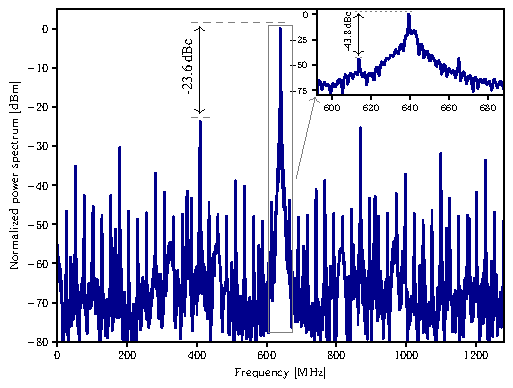
\includegraphics[scale=1, width=12.8cm, height=10.5cm]{slike/fll_spectrum_ppt.pdf} };
    % 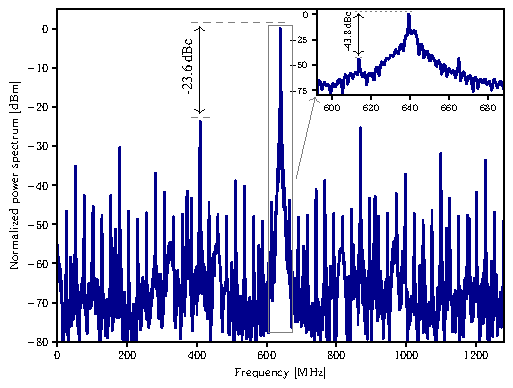
\includegraphics[scale=1, width=12.8cm, height=10.5cm]{slike/fll_spectrum_ppt.pdf}
    	%\draw[<->] (-7.25,-7.3) -- (-7.25,6.8) node[midway, left=0.2, above=0.05, rotate=90] {\footnotesize 70,11\,\textmu m};
    	%\draw[<->] (-6.73,-7.9) -- (7,-7.9) node[midway, right=0.1, below=0.02] {\footnotesize 67,825\,\textmu m};
	\draw (0.6,-4.85) node[rectangle, fill=white]{\footnotesize Учестаност [MHz]};
	\draw (-6.1,0.5) node[rectangle, fill=white, rotate=90]{\footnotesize Нормализовани спектар снаге [dBm]};
    \end{tikzpicture}
    \caption{Спектар снаге \FLL-a, са учестаношћу носиоца 640\,MHz, најјачим нивоом непожељног сигнала (у средини лијево) на -23,6\,dBc, и највећим непожељним сигналом референтне учестаности унутар 640 $\pm$ 16\,MHz (горе десно, зумирано) на нивоу -43,8\,dBc.}
    \label{FLL_spectrum}
\end{figure}
Подаци са графика су добијени из дигиталне симулације на нивоу логичких кола, трајања 15\,\textmu m, која укључује идеалан бешумни модел \DCO-а написан у SystemVerilog-у. Излаз симулације је потпуно детерминистички квадратни талас састављен од јединица и нула, одабран са учестаношћу 10\,GHz, и сачуван за даљу обраду.\par
Највећа вриједност на графику представља учестаност осциловања \FLL-а, односно учестаност носиоца \engl{Carrier Frequency}. Ниво највећег непожељног тона је $-23,6\,\text{dBc}$, што је више од два реда величине испод нивоа учестаности носиоца ($0\,\text{dBc}$). У зумираној области, може се видјети непожељан сигнал унутар референтне учестаности и то лијево и десно од носиоца са помјерајем \engl{Offset} од 16\,MHz, чији је најјачи ниво на $-43,8\,\text{dBc}$.

\subsection{Фазни шум дигитално контролисаног осцилатора}
Због насумичних фазних одступања, спектар снаге реалног осцилатора се такође шири на учестаности око учестаности носиоца, $f_\text{osc}$. Извори насумичних фазних поремећаја~\cite{Milovanovic:8190103} у виду шума треперења и топлотног шума се манифестују као $1/f^3$ and $1/f^2$ области, респективно, у добијеном профилу фазног шума на Слици~\ref{Phase_noise}. Приказани резултати су добијени у типичним \PVT\ условима, са вриједношћу напона напајања \DCO-a ($V_\text{DDL}$) од 1,1\,V, и вриједности учестаности носиоца ($f_\text{osc}$) од 640\,MHz.
\begin{figure}[!ht]
    \centering
    \begin{tikzpicture}[scale=1]
    \pgfplotsset{%
        width=11cm,
        height=9cm
    }
    \definecolor{darkgray176}{RGB}{176,176,176}
    \definecolor{steelblue31119180}{RGB}{31,119,180}
    \begin{axis}[
    log basis x={10},
    tick align=outside,
    tick pos=left,
    x grid style={darkgray176},
    xlabel={Помјерај учестаности од носиоца [Hz]},
    xmajorgrids,
    xmin=10000, xmax=100000000,
    xmode=log,
    xtick style={color=black},
    xtick={100,1000,10000,100000,1000000,10000000,100000000,1000000000},
    xticklabels={
      \(\displaystyle {10^{2}}\),
      \(\displaystyle {10^{3}}\),
      \(\displaystyle {10^{4}}\),
      \(\displaystyle {10^{5}}\),
      \(\displaystyle {10^{6}}\),
      \(\displaystyle {10^{7}}\),
      \(\displaystyle {10^{8}}\),
      \(\displaystyle {10^{9}}\)
    },
    y grid style={darkgray176},
    ylabel={Фазни шум [dBc/Hz]},
    ymajorgrids,
    %ymin=-156.5901503474, ymax=-15.4034960045436,
    ymin=-150.17257515, ymax=-50.0,    
    ytick style={color=black},
    %
    ytick={-150,-140,...,-20},
    line width = 1pt,
    x axis line style = {line width=0.2pt},
    y axis line style = {line width=0.2pt},
    x grid style = {line width=0.2pt},
    y grid style = {line width=0.2pt},
    %legend pos=outer north east,
    %legend style={at={(1.1,0.7)}, font=\scriptsize, line width=0.5pt},
    tick label style={font=\footnotesize},
    label style={font=\footnotesize}
    ]
    \addplot [PineGreen]
    table {%
    10000 -52.6381768941155
    12589.2541179657 -55.7132480787789
    15848.9319245815 -58.7860682107979
    19952.6231496334 -61.856128123895
    25118.8643151522 -64.9227826538102
    31622.7766016722 -67.9852160906684
    39810.7170553207 -71.0424001570802
    50118.7233626842 -74.0930436989566
    63095.7344480753 -77.1355337499079
    79432.8234723806 -80.1678685406367
    100000 -83.1875845985934
    125892.541179419 -86.1916825555938
    158489.319246054 -89.1765598464399
    199526.23149693 -92.1379631181438
    251188.643150926 -95.0709784418529
    316227.766016841 -97.9700820556038
    398107.170553446 -100.829276057501
    501187.233627319 -103.642328917992
    630957.344480157 -106.403126592204
    794328.234724283 -109.106115174851    
    };
    \addplot [Violet]
    table {%      
    794328.234724283 -109.106115174851
    1000000 -111.746784125744
    1258925.41179419 -114.322110058501
    1584893.19246113 -116.830868723868
    1995262.31496882 -119.27373766871
    2511886.43150961 -121.653152778972
    3162277.66016841 -123.972933994157
    3981071.70553493 -126.237735872754
    5011872.33627272 -128.45239141105
    6309573.44480193 -130.621198461401
    7943282.34724283 -132.747156786796 
    10000000 -134.831115669537
    12589254.1179417 -136.870754816228
    15848931.9246112 -138.859319431495
    19952623.1496888 -140.784108096918
    25118864.3150959 -142.624946051807
    31622776.6016839 -144.353347880552
    39810717.0553498 -145.933714229406
    50118723.3627273 -147.328173330804
    63095734.4480195 -148.505453388476
    79432823.4724283 -149.450975613148
    95000000.00 -150.0
	100000000 -150.172575149997    
    };
    \end{axis}
    \draw[->]  (5.5, 4.6) -- (4.5, 3.1);
    \node[] at (5.5, 4.8) {\footnotesize угаона фреквенција};    
    \end{tikzpicture}
	\caption{Спектар фазног шума \DCO-a: област шума треперења (лијево), област топлотног шума (десно), и угаона фреквенција од $\approx$\,800\,kHz.}
	\label{Phase_noise}
\end{figure}


\section{Пајтон модел \FLL-а} \label{section:python_model}
У сврху практичнијег симулирања и бољег предвиђања понашања \FLL-а при различитим условима рада, направљен је основни Пајтон модел цјелокупног \FLL-а. Предност посједовања таквог модела јесте што се одређене карактеристике конкретног дизајна могу параметризовати и затим је, у зависности од тога колико услова модел покрива, могуће веома брзо добити мање или више вјеродостојан резултат понашања тог дизајна, умјесто да се, с друге стране, мијења дизајн и додатним симулацијама утврђују карактеристике под различитим условима, па тек затим пређе на симулације крајњег понашања, што доста успорава процес пројектовања. Конкретна имплементација Пајтон модела \FLL-а из овог рада обухвата, поред параметара самог \FLL-а, и параметризовану почетну учестаност \DCO-а и његову резолуцију, што омогућава тренутно добијање резултата симулације. Треба напоменути да направљени модел предвиђа константне услове рада тј. параметри модела се не мијењају током времена, односно кроз итерације у петљи модела, и да модел не покрива све услове рада. То значи да резултати приказани у наставку не морају да одговарају резултатима из RTL симулација или симулација на нивоу логичких кола, већ су ту да пројектанта наведу на исправну употребу одређених константи (као што су \PID\ константе) или да му помогну око одабира компоненти дизајна чије појединачно понашање му је већ познато и може да се параметризује (рецимо понашање \DCO-а). \par

\subsection{Пајтон код} \label{section:python_model:source}
У наставку ће бити приказан изворни Пајтон код модела, са логиком и називима промјенљивих који углавном одговарају онима из SystemVerilog хардверске имплементације. Биће наведени само листинзи, без детаљног објашњења кода, јер је већина принципа рада већ анализирана при опису хардверске имплементације. Прегледности ради, код је подијељен у класе и то:
\begin{itemize}
	\item \prog{fll} - Класа \FLL\ компоненте (\lstlistingname~\ref{lst:py:fll}).
	\item \prog{pid} - Класа \PID\ регулатора (\lstlistingname~\ref{lst:py:pid}).
	\item \prog{cnt} - Класа бројача из двостепеног регулатора (\lstlistingname~\ref{lst:py:cnt}).
	\item \prog{dco} - Класа дигитално контролисаног осцилатора (\lstlistingname~\ref{lst:py:dco}).
\end{itemize}
С обзиром да \prog{dco} класа нема хардверску имплементацију у виду SystemVerilog модула, треба напоменути да се логика имплементације софтверског модела ослања на једначину~\ref{f_dco} што се може видјети у~\lstlistingname{у}~\ref{lst:py:dco}.
\begin{lstlisting}[language=Python, caption={Имплементација модела \FLL\ компоненте.}, label={lst:py:fll}]
from dco import dco
from cnt import cnt
from pid import pid

class fll:
    def __init__(self,
                 # Inputs from design
                 CW,               # control word width
                 clk_ref_i,        # reference clock
                 clk_ref_en_i,     # reference clock enable
                 rst_ni,           # async reset
                 clk_mult_i,       # reference frequency multiplier [40]
                 dco_pwr_sel_i,    # DCO clock output power supply selection: VDDL/VDD [0/1]
                 dco_ctrl_man_i,   # manual DCO control word [200]
                 dco_ctrl_mode_i,  # DCO control mode: FIXED/MANUAL/CNT/PID [PID=3/CNT=2]
                 pid_kp_i,         # PID controller proportional constant [0b01000000]
                 pid_ki_i,         # PID controller integral constant [0b01000000]
                 pid_kd_i,         # PID controller derivative constant [0]
                 lock_cnt_i,       # FLL lock counter condition [0b1000]
                 # Additional input parameters
                 k_dco,            # DCO frequency resolution
                 clk_dco_init):    # DCO initial frequency (dco_ctrl=0) 
        """
        Frequency-locked loop (FLL) is a negative feedback control system that locks the output frequency signal to the target frequency. Principally, it continuously controls the oscillator frequency in an automated way until its output frequency matches the target value, after which that value is maintained at the output.
        """
        # Inputs from design
        self.CW = CW
        self.clk_ref_i = clk_ref_i 
        self.clk_ref_en_i = clk_ref_en_i
        self.rst_ni = rst_ni
        self.clk_mult_i = clk_mult_i
        self.dco_pwr_sel_i = dco_pwr_sel_i  
        self.dco_ctrl_man_i = dco_ctrl_man_i
        self.dco_ctrl_mode_i = dco_ctrl_mode_i 
        self.pid_kp_i = pid_kp_i
        self.pid_ki_i = pid_ki_i
        self.pid_kd_i = pid_kd_i
        self.lock_cnt_i = lock_cnt_i
        # Additional input parameters
        self.k_dco = k_dco
        self.clk_dco_init = clk_dco_init
        # Component instantiation
        self.dco_inst = dco(k_dco=self.k_dco,
                            init_freq=self.clk_dco_init)
        self.cnt_inst = cnt()
        self.pid_inst = pid(rst_ni=self.rst_ni,
                            kp_i=self.pid_kp_i,
                            ki_i=self.pid_ki_i,
                            kd_i=self.pid_kd_i,
                            setpoint_i=self.clk_mult_i,
                            feedback_i=self.clk_dco_init//self.clk_ref_i,
                            lock_cnt_i=self.lock_cnt_i)
        # Outputs from design
        self.lock_o = self.clk_dco_init//self.clk_ref_i == self.clk_mult_i
        self.clk_dco_o = self.clk_dco_init

    def run(self,
            rst_ni):
        self.rst_ni = rst_ni

        # Convert control mode integer value to the corresponding binary array (1/0 integers) 
        dco_ctrl_mode_bin_arr = list(map(int, list(bin(self.dco_ctrl_mode_i)[2:][::-1])))

        # PID logic
        self.pid_inst.feedback_i = self.clk_dco_o//self.clk_ref_i
        self.pid_inst.run(rst_ni=self.rst_ni)
        dco_ctrl_pid = self.pid_inst.ctrl_o

        # Bang-bang logic
        #cnt_en_i = 1  # used if you want frequency oscillation in the stable state
        cnt_en_i = not self.pid_inst.lock_o if (self.clk_mult_i != self.clk_dco_o//self.clk_ref_i) else 0
        cnt_up_down = 1 if (self.clk_mult_i > self.clk_dco_o//self.clk_ref_i) else 0
        self.cnt_inst.run(rst_ni=self.rst_ni,
                          en_i=cnt_en_i and dco_ctrl_mode_bin_arr[1],
                          up_down_i=cnt_up_down)
        dco_ctrl_cnt = self.cnt_inst.cnt_o

        # Control preprocessing
        dco_ctrl_man = self.dco_ctrl_man_i if (dco_ctrl_mode_bin_arr[0]) else 203
        dco_ctrl_auto = dco_ctrl_pid if (dco_ctrl_mode_bin_arr[0]) else dco_ctrl_cnt
        dco_ctrl = dco_ctrl_auto if (dco_ctrl_mode_bin_arr[1]) else dco_ctrl_man

        # DCO logic
        self.dco_inst.run(ctrl=dco_ctrl)

        # FLL outputs setup
        self.clk_dco_o = int(self.dco_inst.freq_out)
        self.lock_o = self.pid_inst.lock_o
\end{lstlisting}
\begin{lstlisting}[language=Python, caption={Имплементација класе \PID\ регулатора.}, label={lst:py:pid}]
import copy

INT_WIDTH = 8                   # width of output control signal
FX_INT_WIDTH = 12               # integer part width of PID sum (Q12.6)
FX_DEC_WIDTH = 6                # decimal part width of PID sum (Q12.6)
CTRL_WIDTH = FX_INT_WIDTH + FX_DEC_WIDTH  # total width of PID sum

class pid:
    def __init__(self,
                 rst_ni,
                 kp_i,
                 ki_i,
                 kd_i,
                 setpoint_i,
                 feedback_i,
                 lock_cnt_i):
        self.rst_ni = rst_ni
        self.kp_i = kp_i
        self.ki_i = ki_i
        self.kd_i = kd_i
        self.setpoint_i = setpoint_i
        self.feedback_i = feedback_i
        self.lock_cnt_i = lock_cnt_i
        self.ctrl_o = 0
        self.lock_o = 0
        self.err_eq0_cnt = 0
        self.integ = 0
        self.err = setpoint_i - feedback_i
        self.err_prev = 0
        self.ctrl_pid = 0

    def run(self,
            rst_ni):
        self.rst_ni = rst_ni

        if (not self.rst_ni):
            self.err_eq0_cnt = 0
        else:
            if ((self.err == 0) and (self.err_eq0_cnt < self.lock_cnt_i)):
                self.err_eq0_cnt += 1

        prop = 0
        deriv = 0
        self.err = self.setpoint_i - self.feedback_i
        err_diff = self.err - self.err_prev

        if (not self.rst_ni):
            prop = 0
            self.integ = 0
            deriv = 0
            self.err_prev = 0
            self.ctrl_pid = 0
            self.lock_o = 0
        else:
            prop = self.kp_i * self.err
            self.integ += self.ki_i * self.err
            deriv = self.kd_i * err_diff
            self.err_prev = copy.deepcopy(self.err)
            if ((self.err == 0) and (self.err_eq0_cnt == self.lock_cnt_i) and (self.lock_cnt_i != 0)):
                self.lock_o = 1
            if (not self.lock_o):
                self.ctrl_pid = prop + self.integ + deriv

        self.ctrl_o = int(format(int(self.ctrl_pid), '0'+str(CTRL_WIDTH)+'b')[FX_INT_WIDTH-INT_WIDTH:FX_INT_WIDTH], 2)
\end{lstlisting}
\begin{lstlisting}[language=Python, caption={Имплементација класе бројача двостепеног регулатора.}, label={lst:py:cnt}]
class cnt:
    def __init__(self):
        self.cnt_o = 0
        self.default_val = 0

    def run(self,
            rst_ni,
            en_i,
            up_down_i):
        if (not rst_ni):
            self.cnt_o = self.default_val
        else:    
            if (en_i):
                if (up_down_i):
                    self.cnt_o += 1
                else:
                    self.cnt_o -= 1
        return self.cnt_o
\end{lstlisting}
\begin{lstlisting}[language=Python, caption={Имплементација класе дигитално контролисаног осцилатора.}, label={lst:py:dco}]
class dco:
    def __init__(self,
                 k_dco,
                 init_freq):
        self.k_dco = k_dco
        self.init_freq = init_freq
        self.freq_out = init_freq

    def run(self,
            ctrl):
        self.freq_out = self.init_freq + self.k_dco * ctrl
\end{lstlisting}

\subsection{Поређење рада различитих управљачких режима} \label{section:python_model:pid_vs_cnt}
\figurename~\ref{fig:py:pid_vs_cnt_1} приказује одзив софтверског модела \FLL-а при раду у \PID\ и двостепеном управљачком режиму рада. У конкретној симулацији коришћено је понашање \DCO-а добијено симулацијом у типичним условима рада, па су при инстанцирању софтверског модела \FLL-а коришћени подаци из Табеле~\ref{tab:frequency_ranges_and_average_kdco}, односно $K_\text{DCO}$=2,8\,MHz и $f_\text{min}$=42\,MHz за почетну учестаност. Конкретна вриједност учестаности која се овом симулацијом достиже у оба режима је 641,2\,MHz. У \PID\ режиму модел до те учестаности стиже након 28 итерација, док му је са двостепеним управљачким режимом потребно 214 итерација. \par 
\begin{figure*}[!ht]%[!b]
    \centering

    %\def \SSLineStyle {solid}
    %\def \TTLineStyle {dashed}
    %\def \FFLineStyle {dotted}
    
    \begin{tikzpicture}[scale=1]
    \pgfplotsset{%
        width=15.5cm,
        height=10cm
    }
    
    \definecolor{darkgray176}{RGB}{176,176,176}
    \definecolor{darkorange25512714}{RGB}{255,127,14}
    %\definecolor{forestgreen4416044}{RGB}{44,160,44}
    \definecolor{steelblue31119180}{RGB}{31,119,180}
    
    \begin{axis}[
    tick align=outside,
    tick pos=left,
    x grid style={darkgray176},
    xlabel={Број итерација},
    xmajorgrids,
    xmin=0, xmax=250,
    xtick style={color=black},
    y grid style={darkgray176},
    ylabel={Учестаност осциловања [MHz]},
    ymajorgrids,
    ymin=0, ymax=650,
    ytick style={color=black},
    %
    %ytick={0,0.2,...,1.2},
    xlabel style={align=center,text width=8cm},
    line width = 1pt,
    x axis line style = {line width=0.2pt},
    y axis line style = {line width=0.2pt},
    x grid style = {line width=0.2pt},
    y grid style = {line width=0.2pt},
    %legend pos=north west,
    %legend style={legend image post style={mark options={scale=0.7}}, cells={anchor=west}, at={(0.69,1)}, font=\tiny, line width=0.5pt, legend reversed=true},
    legend style={legend image post style={scale=0.82}, cells={anchor=west}, at={(1.0,0.1125)}, font=\scriptsize, line width=0.5pt, legend reversed=true},
    tick label style={font=\footnotesize},
    label style={font=\footnotesize}
    ]
    %\addplot [steelblue31119180, mark=*, mark options={scale=0.5, mark repeat=15}]
    %\addplot [steelblue31119180, solid]
    \addplot [semithick, steelblue31119180, const plot mark right]
    table {%
    0 44.8
    1 47.6
    2 50.4
    3 53.2
    4 56
    5 58.8
    6 61.6
    7 64.4
    8 67.2
    9 70
    10 72.8
    11 75.6
    12 78.4
    13 81.2
    14 84
    15 86.8
    16 89.6
    17 92.4
    18 95.2
    19 98
    20 100.8
    21 103.6
    22 106.4
    23 109.2
    24 112
    25 114.8
    26 117.6
    27 120.4
    28 123.2
    29 126
    30 128.8
    31 131.6
    32 134.4
    33 137.2
    34 140
    35 142.8
    36 145.6
    37 148.4
    38 151.2
    39 154
    40 156.8
    41 159.6
    42 162.4
    43 165.2
    44 168
    45 170.8
    46 173.6
    47 176.4
    48 179.2
    49 182
    50 184.8
    51 187.6
    52 190.4
    53 193.2
    54 196
    55 198.8
    56 201.6
    57 204.4
    58 207.2
    59 210
    60 212.8
    61 215.6
    62 218.4
    63 221.2
    64 224
    65 226.8
    66 229.6
    67 232.4
    68 235.2
    69 238
    70 240.8
    71 243.6
    72 246.4
    73 249.2
    74 252
    75 254.8
    76 257.6
    77 260.4
    78 263.2
    79 266
    80 268.8
    81 271.6
    82 274.4
    83 277.2
    84 280
    85 282.8
    86 285.6
    87 288.4
    88 291.2
    89 294
    90 296.8
    91 299.6
    92 302.4
    93 305.2
    94 308
    95 310.8
    96 313.6
    97 316.4
    98 319.2
    99 322
    100 324.8
    101 327.6
    102 330.4
    103 333.2
    104 336
    105 338.8
    106 341.6
    107 344.4
    108 347.2
    109 350
    110 352.8
    111 355.6
    112 358.4
    113 361.2
    114 364
    115 366.8
    116 369.6
    117 372.4
    118 375.2
    119 378
    120 380.8
    121 383.6
    122 386.4
    123 389.2
    124 392
    125 394.8
    126 397.6
    127 400.4
    128 403.2
    129 406
    130 408.8
    131 411.6
    132 414.4
    133 417.2
    134 420
    135 422.8
    136 425.6
    137 428.4
    138 431.2
    139 434
    140 436.8
    141 439.6
    142 442.4
    143 445.2
    144 448
    145 450.8
    146 453.6
    147 456.4
    148 459.2
    149 462
    150 464.8
    151 467.6
    152 470.4
    153 473.2
    154 476
    155 478.8
    156 481.6
    157 484.4
    158 487.2
    159 490
    160 492.8
    161 495.6
    162 498.4
    163 501.2
    164 504
    165 506.8
    166 509.6
    167 512.4
    168 515.2
    169 518
    170 520.8
    171 523.6
    172 526.4
    173 529.2
    174 532
    175 534.8
    176 537.6
    177 540.4
    178 543.2
    179 546
    180 548.8
    181 551.6
    182 554.4
    183 557.2
    184 560
    185 562.8
    186 565.6
    187 568.4
    188 571.2
    189 574
    190 576.8
    191 579.6
    192 582.4
    193 585.2
    194 588
    195 590.8
    196 593.6
    197 596.4
    198 599.2
    199 602
    200 604.8
    201 607.6
    202 610.4
    203 613.2
    204 616
    205 618.8
    206 621.6
    207 624.4
    208 627.2
    209 630
    210 632.8
    211 635.6
    212 638.4
    213 641.2
    214 641.2
    215 641.2
    216 641.2
    217 641.2
    218 641.2
    219 641.2
    220 641.2
    221 641.2
    222 641.2
    223 641.2
    224 641.2
    225 641.2
    226 641.2
    227 641.2
    228 641.2
    229 641.2
    230 641.2
    231 641.2
    232 641.2
    233 641.2
    234 641.2
    235 641.2
    236 641.2
    237 641.2
    238 641.2
    239 641.2
    240 641.2
    241 641.2
    242 641.2
    243 641.2
    244 641.2
    245 641.2
    246 641.2
    247 641.2
    248 641.2
    249 641.2
    250 641.2
    };
    \addlegendentry{Двостепени контролер}
    %\addlegendentry{$K_\text{p}\text{=}64, K_\text{i}\text{=}64, K_\text{d}\text{=}64$}
    %\addplot [darkorange25512714, mark=square*, mark options={scale=0.5, mark repeat=15}]
    \addplot [semithick, darkorange25512714, const plot mark right]
    table {%
    0 240.8
    1 271.6
    2 333.2
    3 375.2
    4 411.6
    5 445.2
    6 473.2
    7 498.4
    8 515.2
    9 534.8
    10 548.8
    11 562.8
    12 574
    13 588
    14 593.6
    15 599.2
    16 607.6
    17 616
    18 618.8
    19 624.4
    20 624.4
    21 627.2
    22 630
    23 630
    24 632.8
    25 635.6
    26 638.4
    27 641.2
    28 638.4
    29 644
    30 641.2
    31 641.2
    32 641.2
    33 641.2
    34 641.2
    35 641.2
    36 641.2
    37 641.2
    38 641.2
    39 641.2
    40 641.2
    41 641.2
    42 641.2
    43 641.2
    44 641.2
    45 641.2
    46 641.2
    47 641.2
    48 641.2
    49 641.2
    50 641.2
    51 641.2
    52 641.2
    53 641.2
    54 641.2
    55 641.2
    56 641.2
    57 641.2
    58 641.2
    59 641.2
    60 641.2
    61 641.2
    62 641.2
    63 641.2
    64 641.2
    65 641.2
    66 641.2
    67 641.2
    68 641.2
    69 641.2
    70 641.2
    71 641.2
    72 641.2
    73 641.2
    74 641.2
    75 641.2
    76 641.2
    77 641.2
    78 641.2
    79 641.2
    80 641.2
    81 641.2
    82 641.2
    83 641.2
    84 641.2
    85 641.2
    86 641.2
    87 641.2
    88 641.2
    89 641.2
    90 641.2
    91 641.2
    92 641.2
    93 641.2
    94 641.2
    95 641.2
    96 641.2
    97 641.2
    98 641.2
    99 641.2
    100 641.2
    101 641.2
    102 641.2
    103 641.2
    104 641.2
    105 641.2
    106 641.2
    107 641.2
    108 641.2
    109 641.2
    110 641.2
    111 641.2
    112 641.2
    113 641.2
    114 641.2
    115 641.2
    116 641.2
    117 641.2
    118 641.2
    119 641.2
    120 641.2
    121 641.2
    122 641.2
    123 641.2
    124 641.2
    125 641.2
    126 641.2
    127 641.2
    128 641.2
    129 641.2
    130 641.2
    131 641.2
    132 641.2
    133 641.2
    134 641.2
    135 641.2
    136 641.2
    137 641.2
    138 641.2
    139 641.2
    140 641.2
    141 641.2
    142 641.2
    143 641.2
    144 641.2
    145 641.2
    146 641.2
    147 641.2
    148 641.2
    149 641.2
    150 641.2
    151 641.2
    152 641.2
    153 641.2
    154 641.2
    155 641.2
    156 641.2
    157 641.2
    158 641.2
    159 641.2
    160 641.2
    161 641.2
    162 641.2
    163 641.2
    164 641.2
    165 641.2
    166 641.2
    167 641.2
    168 641.2
    169 641.2
    170 641.2
    171 641.2
    172 641.2
    173 641.2
    174 641.2
    175 641.2
    176 641.2
    177 641.2
    178 641.2
    179 641.2
    180 641.2
    181 641.2
    182 641.2
    183 641.2
    184 641.2
    185 641.2
    186 641.2
    187 641.2
    188 641.2
    189 641.2
    190 641.2
    191 641.2
    192 641.2
    193 641.2
    194 641.2
    195 641.2
    196 641.2
    197 641.2
    198 641.2
    199 641.2
    200 641.2
    201 641.2
    202 641.2
    203 641.2
    204 641.2
    205 641.2
    206 641.2
    207 641.2
    208 641.2
    209 641.2
    210 641.2
    211 641.2
    212 641.2
    213 641.2
    214 641.2
    215 641.2
    216 641.2
    217 641.2
    218 641.2
    219 641.2
    220 641.2
    221 641.2
    222 641.2
    223 641.2
    224 641.2
    225 641.2
    226 641.2
    227 641.2
    228 641.2
    229 641.2
    230 641.2
    231 641.2
    232 641.2
    233 641.2
    234 641.2
    235 641.2
    236 641.2
    237 641.2
    238 641.2
    239 641.2
    240 641.2
    241 641.2
    242 641.2
    243 641.2
    244 641.2
    245 641.2
    246 641.2
    247 641.2
    248 641.2
    249 641.2
    250 641.2
    };
    \addlegendentry{\PID\ контролер (\P=15, \I=15, \D=0)}
    %\addlegendentry{$K_\text{p}\text{=}64, K_\text{i}\text{=}64, K_\text{d}\text{=}64$}
    %\addplot [forestgreen4416044, mark=triangle*, mark options={scale=0.5, mark repeat=15}]
    \end{axis}
    \end{tikzpicture}
    \caption{Одзив модела у \PID\ и двостепеном режиму рада.}
    \label{fig:py:pid_vs_cnt_1}
\end{figure*}

У поглављу~\ref{section:bang_bang} поменута је појава осциловања учестаности у стабилном стању када \FLL\ ради у двостепеном режиму. На Слици~\ref{fig:py:pid_vs_cnt_1} те осцилације не постоје, а проблем је ријешен условним довођењем \prog{pid.lock\_o} сигнала на \prog{cnt.en\_i} улаз бројача двостепеног регулатора. Логика имплементације се налази на линији \prog{75}~\lstlistingname{а}~\ref{lst:py:fll}. Да би се ипак показало како те осцилације изгледају, довољно је само закоментарисати поменуту линију, а одкоментарисати линију \prog{74}. Тиме се добија одзив као на Слици~\ref{fig:py:pid_vs_cnt_2}, гдје учестаност у стабилном стању, при коришћењу двостепеног регулатора, варира између 638,4\,MHz и 641,2\,MHz (примјећујемо да разлика између поменутих вриједности представља вриједност резолуције, $K_\text{DCO}$=2,8\,MHz).
\begin{figure*}[!ht]%[!b]
    \centering

    %\begin{tikzpicture}[spy using outlines={rectangle, red, dashed, fill=white, magnification=4, height=1.2cm, width=7cm, connect spies}]
    \begin{tikzpicture}[spy using overlays={rectangle, dashed, green!60, magnification=4, height=1.2cm, width=7cm, connect spies}]
    \pgfplotsset{%
        width=15.5cm,
        height=10cm
    }
    
    \definecolor{darkgray176}{RGB}{176,176,176}
    \definecolor{darkorange25512714}{RGB}{255,127,14}
    \definecolor{steelblue31119180}{RGB}{31,119,180}
    
    \begin{axis}[
    tick align=outside,
    tick pos=left,
    x grid style={darkgray176},
    xlabel={Број итерација/корака},
    xmajorgrids,
    xmin=0, xmax=250,
    xtick style={color=black},
    y grid style={darkgray176},
    ylabel={Учестаност осциловања [MHz]},
    ymajorgrids,
    ymin=0, ymax=650,
    ytick style={color=black},
    %
    %ytick={0,0.2,...,1.2},
    xlabel style={align=center,text width=8cm},
    line width = 1pt,
    x axis line style = {line width=0.2pt},
    y axis line style = {line width=0.2pt},
    x grid style = {line width=0.2pt},
    y grid style = {line width=0.2pt},
    legend style={legend image post style={scale=0.82}, cells={anchor=west}, at={(0.7,0.113)}, font=\scriptsize, line width=0.5pt, legend reversed=true},
    tick label style={font=\footnotesize},
    label style={font=\footnotesize}
    ]
    \addplot [semithick, steelblue31119180, const plot mark right]
    table {%
    0 44.8
    1 47.6
    2 50.4
    3 53.2
    4 56
    5 58.8
    6 61.6
    7 64.4
    8 67.2
    9 70
    10 72.8
    11 75.6
    12 78.4
    13 81.2
    14 84
    15 86.8
    16 89.6
    17 92.4
    18 95.2
    19 98
    20 100.8
    21 103.6
    22 106.4
    23 109.2
    24 112
    25 114.8
    26 117.6
    27 120.4
    28 123.2
    29 126
    30 128.8
    31 131.6
    32 134.4
    33 137.2
    34 140
    35 142.8
    36 145.6
    37 148.4
    38 151.2
    39 154
    40 156.8
    41 159.6
    42 162.4
    43 165.2
    44 168
    45 170.8
    46 173.6
    47 176.4
    48 179.2
    49 182
    50 184.8
    51 187.6
    52 190.4
    53 193.2
    54 196
    55 198.8
    56 201.6
    57 204.4
    58 207.2
    59 210
    60 212.8
    61 215.6
    62 218.4
    63 221.2
    64 224
    65 226.8
    66 229.6
    67 232.4
    68 235.2
    69 238
    70 240.8
    71 243.6
    72 246.4
    73 249.2
    74 252
    75 254.8
    76 257.6
    77 260.4
    78 263.2
    79 266
    80 268.8
    81 271.6
    82 274.4
    83 277.2
    84 280
    85 282.8
    86 285.6
    87 288.4
    88 291.2
    89 294
    90 296.8
    91 299.6
    92 302.4
    93 305.2
    94 308
    95 310.8
    96 313.6
    97 316.4
    98 319.2
    99 322
    100 324.8
    101 327.6
    102 330.4
    103 333.2
    104 336
    105 338.8
    106 341.6
    107 344.4
    108 347.2
    109 350
    110 352.8
    111 355.6
    112 358.4
    113 361.2
    114 364
    115 366.8
    116 369.6
    117 372.4
    118 375.2
    119 378
    120 380.8
    121 383.6
    122 386.4
    123 389.2
    124 392
    125 394.8
    126 397.6
    127 400.4
    128 403.2
    129 406
    130 408.8
    131 411.6
    132 414.4
    133 417.2
    134 420
    135 422.8
    136 425.6
    137 428.4
    138 431.2
    139 434
    140 436.8
    141 439.6
    142 442.4
    143 445.2
    144 448
    145 450.8
    146 453.6
    147 456.4
    148 459.2
    149 462
    150 464.8
    151 467.6
    152 470.4
    153 473.2
    154 476
    155 478.8
    156 481.6
    157 484.4
    158 487.2
    159 490
    160 492.8
    161 495.6
    162 498.4
    163 501.2
    164 504
    165 506.8
    166 509.6
    167 512.4
    168 515.2
    169 518
    170 520.8
    171 523.6
    172 526.4
    173 529.2
    174 532
    175 534.8
    176 537.6
    177 540.4
    178 543.2
    179 546
    180 548.8
    181 551.6
    182 554.4
    183 557.2
    184 560
    185 562.8
    186 565.6
    187 568.4
    188 571.2
    189 574
    190 576.8
    191 579.6
    192 582.4
    193 585.2
    194 588
    195 590.8
    196 593.6
    197 596.4
    198 599.2
    199 602
    200 604.8
    201 607.6
    202 610.4
    203 613.2
    204 616
    205 618.8
    206 621.6
    207 624.4
    208 627.2
    209 630
    210 632.8
    211 635.6
    212 638.4
    213 641.2
    214 638.4
    215 641.2
    216 638.4
    217 641.2
    218 638.4
    219 641.2
    220 638.4
    221 641.2
    222 638.4
    223 641.2
    224 638.4
    225 641.2
    226 638.4
    227 641.2
    228 638.4
    229 641.2
    230 638.4
    231 641.2
    232 638.4
    233 641.2
    234 638.4
    235 641.2
    236 638.4
    237 641.2
    238 638.4
    239 641.2
    240 638.4
    241 641.2
    242 638.4
    243 641.2
    244 638.4
    245 641.2
    246 638.4
    247 641.2
    248 638.4
    249 641.2
    250 638.4
    };
    \addlegendentry{Двостепени регулатор}
    \addplot [semithick, darkorange25512714, const plot mark right]
    table {%
    0 240.8
    1 271.6
    2 333.2
    3 375.2
    4 411.6
    5 445.2
    6 473.2
    7 498.4
    8 515.2
    9 534.8
    10 548.8
    11 562.8
    12 574
    13 588
    14 593.6
    15 599.2
    16 607.6
    17 616
    18 618.8
    19 624.4
    20 624.4
    21 627.2
    22 630
    23 630
    24 632.8
    25 635.6
    26 638.4
    27 641.2
    28 638.4
    29 644
    30 641.2
    31 641.2
    32 641.2
    33 641.2
    34 641.2
    35 641.2
    36 641.2
    37 641.2
    38 641.2
    39 641.2
    40 641.2
    41 641.2
    42 641.2
    43 641.2
    44 641.2
    45 641.2
    46 641.2
    47 641.2
    48 641.2
    49 641.2
    50 641.2
    51 641.2
    52 641.2
    53 641.2
    54 641.2
    55 641.2
    56 641.2
    57 641.2
    58 641.2
    59 641.2
    60 641.2
    61 641.2
    62 641.2
    63 641.2
    64 641.2
    65 641.2
    66 641.2
    67 641.2
    68 641.2
    69 641.2
    70 641.2
    71 641.2
    72 641.2
    73 641.2
    74 641.2
    75 641.2
    76 641.2
    77 641.2
    78 641.2
    79 641.2
    80 641.2
    81 641.2
    82 641.2
    83 641.2
    84 641.2
    85 641.2
    86 641.2
    87 641.2
    88 641.2
    89 641.2
    90 641.2
    91 641.2
    92 641.2
    93 641.2
    94 641.2
    95 641.2
    96 641.2
    97 641.2
    98 641.2
    99 641.2
    100 641.2
    101 641.2
    102 641.2
    103 641.2
    104 641.2
    105 641.2
    106 641.2
    107 641.2
    108 641.2
    109 641.2
    110 641.2
    111 641.2
    112 641.2
    113 641.2
    114 641.2
    115 641.2
    116 641.2
    117 641.2
    118 641.2
    119 641.2
    120 641.2
    121 641.2
    122 641.2
    123 641.2
    124 641.2
    125 641.2
    126 641.2
    127 641.2
    128 641.2
    129 641.2
    130 641.2
    131 641.2
    132 641.2
    133 641.2
    134 641.2
    135 641.2
    136 641.2
    137 641.2
    138 641.2
    139 641.2
    140 641.2
    141 641.2
    142 641.2
    143 641.2
    144 641.2
    145 641.2
    146 641.2
    147 641.2
    148 641.2
    149 641.2
    150 641.2
    151 641.2
    152 641.2
    153 641.2
    154 641.2
    155 641.2
    156 641.2
    157 641.2
    158 641.2
    159 641.2
    160 641.2
    161 641.2
    162 641.2
    163 641.2
    164 641.2
    165 641.2
    166 641.2
    167 641.2
    168 641.2
    169 641.2
    170 641.2
    171 641.2
    172 641.2
    173 641.2
    174 641.2
    175 641.2
    176 641.2
    177 641.2
    178 641.2
    179 641.2
    180 641.2
    181 641.2
    182 641.2
    183 641.2
    184 641.2
    185 641.2
    186 641.2
    187 641.2
    188 641.2
    189 641.2
    190 641.2
    191 641.2
    192 641.2
    193 641.2
    194 641.2
    195 641.2
    196 641.2
    197 641.2
    198 641.2
    199 641.2
    200 641.2
    201 641.2
    202 641.2
    203 641.2
    204 641.2
    205 641.2
    206 641.2
    207 641.2
    208 641.2
    209 641.2
    210 641.2
    211 641.2
    212 641.2
    213 641.2
    214 641.2
    215 641.2
    216 641.2
    217 641.2
    218 641.2
    219 641.2
    220 641.2
    221 641.2
    222 641.2
    223 641.2
    224 641.2
    225 641.2
    226 641.2
    227 641.2
    228 641.2
    229 641.2
    230 641.2
    231 641.2
    232 641.2
    233 641.2
    234 641.2
    235 641.2
    236 641.2
    237 641.2
    238 641.2
    239 641.2
    240 641.2
    241 641.2
    242 641.2
    243 641.2
    244 641.2
    245 641.2
    246 641.2
    247 641.2
    248 641.2
    249 641.2
    250 641.2
    };
    \addlegendentry{\PID\ регулатор (\P=15, \I=15, \D=0)}
    \end{axis}
    \node[draw, rectangle, fill=white, text width=2.2cm] at (6.9,1.46){\scriptsize $K_\text{DCO}$=2,8\,MHz\\$f_\text{min}$=42\,MHz};

    %\begin{scope}
      %[spy using outlines={circle, blue, magnification=3, size=1.5cm, connect spies}]
      %\draw [help lines] (0,0) grid (3,2);
      %\draw [decoration=Koch curve type 1] decorate{ decorate{ decorate{ (0,0) -- (2,0) }}};
      %\spy on (1.6,0.3) in node (zoom) [left] at (3.5,-1.25);
    %\end{scope}
    \draw (12.3,8.25) node[rectangle](zoom){};
    \spy on (zoom.center) in node [left] at (13.2,3.5);

    \end{tikzpicture}
    \caption{Одзив модела у \PID\ и двостепеном режиму рада (са осцилацијама у двостепеном режиму).}
    \label{fig:py:pid_vs_cnt_2}
\end{figure*}


\subsection{Утицај константи \PID\ регулатора на одзив система} \label{section:python_model:pid_tuning}
У овом поглављу биће софтверски симулиран утицај различитих вриједности константи \PID\ регулатора на одзив система. Треба напоменути да одзив не мора у потпуности одговарати стварном одзиву система већ му је циљ помоћи при исправном одабиру константи \PID\ регулатора, а све у циљу добијања најбржег и најправилнијег одзива система у крајњој имплементацији. Као што је објашњено у поглављу~\ref{section:pid}, диференцијална константа није коришћена у имплементацији, па стога неће бити приказан утицај њених различитих вриједности на одзив система. Слике~\ref{fig:py:pid_kp_tuning} и ~\ref{fig:py:pid_ki_tuning} редом приказују утицај различитих вриједности пропорционалне ($K_\text{p}$) и интегралне ($K_\text{i}$) константе на брзину и начин достизања жељене учестаности. \par
\begin{figure*}[!ht]%[!b]
    \centering

    \begin{tikzpicture}[scale=1]
    \pgfplotsset{%
        width=15.5cm,
        height=7.185cm
        %height=7.728cm
	%height=10cm
    }
    
    \definecolor{darkgray176}{RGB}{176,176,176}
    \definecolor{darkorange25512714}{RGB}{255,127,14}
    \definecolor{forestgreen4416044}{RGB}{44,160,44}
    \definecolor{steelblue31119180}{RGB}{31,119,180}
    
    \begin{axis}[
    tick align=outside,
    tick pos=left,
    x grid style={darkgray176},
    xlabel={Број итерација},
    xmajorgrids,
    xmin=0, xmax=60,
    xtick style={color=black},
    y grid style={darkgray176},
    ylabel={Учестаност осциловања [MHz]},
    ymajorgrids,
    ymin=150, ymax=660,
    ytick style={color=black},
    %
    %ytick={0,0.2,...,1.2},
    xlabel style={align=center,text width=8cm},
    line width = 1pt,
    x axis line style = {line width=0.2pt},
    y axis line style = {line width=0.2pt},
    x grid style = {line width=0.2pt},
    y grid style = {line width=0.2pt},
    %legend pos=north west,
    %legend style={legend image post style={mark options={scale=0.7}}, cells={anchor=west}, at={(0.69,1)}, font=\tiny, line width=0.5pt, legend reversed=true},
    legend style={legend image post style={scale=0.82}, cells={anchor=west}, at={(1.0,0.239)}, font=\scriptsize, line width=0.5pt, legend reversed=true},
    tick label style={font=\footnotesize},
    label style={font=\footnotesize}
    ]
    %\addplot [steelblue31119180, mark=*, mark options={scale=0.5, mark repeat=15}]
    %\addplot [steelblue31119180, solid]
    \addplot [semithick, steelblue31119180, const plot mark right]
    table {%
    0 142.8
    1 226.8
    2 294
    3 352.8
    4 400.4
    5 439.6
    6 473.2
    7 501.2
    8 523.6
    9 546
    10 560
    11 574
    12 588
    13 596.4
    14 604.8
    15 613.2
    16 618.8
    17 624.4
    18 627.2
    19 630
    20 630
    21 632.8
    22 635.6
    23 638.4
    24 641.2
    25 641.2
    26 641.2
    27 641.2
    28 641.2
    29 641.2
    30 641.2
    31 641.2
    32 641.2
    33 641.2
    34 641.2
    35 641.2
    36 641.2
    37 641.2
    38 641.2
    39 641.2
    40 641.2
    41 641.2
    42 641.2
    43 641.2
    44 641.2
    45 641.2
    46 641.2
    47 641.2
    48 641.2
    49 641.2
    50 641.2
    51 641.2
    52 641.2
    53 641.2
    54 641.2
    55 641.2
    56 641.2
    57 641.2
    58 641.2
    59 641.2
    60 641.2
    };
    \addlegendentry{\P=0,5, \I=15, \D=0}
    %\addlegendentry{$K_\text{p}\text{=}64, K_\text{i}\text{=}64, K_\text{d}\text{=}64$}
    %\addplot [darkorange25512714, mark=square*, mark options={scale=0.5, mark repeat=15}]
    \addplot [semithick, darkorange25512714, const plot mark right]
    table {%
    0 240.8
    1 271.6
    2 333.2
    3 375.2
    4 411.6
    5 445.2
    6 473.2
    7 498.4
    8 515.2
    9 534.8
    10 548.8
    11 562.8
    12 574
    13 588
    14 593.6
    15 599.2
    16 607.6
    17 616
    18 618.8
    19 624.4
    20 624.4
    21 627.2
    22 630
    23 630
    24 632.8
    25 635.6
    26 638.4
    27 641.2
    28 638.4
    29 644
    30 641.2
    31 641.2
    32 641.2
    33 641.2
    34 641.2
    35 641.2
    36 641.2
    37 641.2
    38 641.2
    39 641.2
    40 641.2
    41 641.2
    42 641.2
    43 641.2
    44 641.2
    45 641.2
    46 641.2
    47 641.2
    48 641.2
    49 641.2
    50 641.2
    51 641.2
    52 641.2
    53 641.2
    54 641.2
    55 641.2
    56 641.2
    57 641.2
    58 641.2
    59 641.2
    60 641.2
    };
    \addlegendentry{\P=15, \I=15, \D=0}
    %\addlegendentry{$K_\text{p}\text{=}64, K_\text{i}\text{=}64, K_\text{d}\text{=}64$}
    %\addplot [forestgreen4416044, mark=triangle*, mark options={scale=0.5, mark repeat=15}]
    \addplot [semithick, forestgreen4416044, const plot mark right]
    table {%
    0 560
    1 210
    2 520.8
    3 333.2
    4 518
    5 406
    6 523.6
    7 467.6
    8 529.2
    9 504
    10 548.8
    11 532
    12 562.8
    13 551.6
    14 579.6
    15 568.4
    16 590.8
    17 590.8
    18 602
    19 599.2
    20 607.6
    21 613.2
    22 607.6
    23 627.2
    24 607.6
    25 638.4
    26 618.8
    27 635.6
    28 627.2
    29 630
    30 632.8
    31 635.6
    32 638.4
    33 638.4
    34 641.2
    35 630
    36 644
    37 632.8
    38 646.8
    39 635.6
    40 649.6
    41 638.4
    42 652.4
    43 641.2
    44 641.2
    45 641.2
    46 641.2
    47 641.2
    48 641.2
    49 641.2
    50 641.2
    51 641.2
    52 641.2
    53 641.2
    54 641.2
    55 641.2
    56 641.2
    57 641.2
    58 641.2
    59 641.2
    60 641.2
    };
    \addlegendentry{\P=63, \I=15, \D=0}
    \end{axis}
    \end{tikzpicture}
    \caption{Одзив модела за различите вриједности пропорционалне константе \PID\ контролера.}
    \label{fig:py:pid_kp_tuning}
\end{figure*}

\begin{figure*}[!ht]%[!b]
    \centering

    \begin{tikzpicture}[scale=1]
    \pgfplotsset{%
        width=15.5cm,
	height=7.185cm
	%height=7.728cm
        %height=10cm
    }
    
    \definecolor{darkgray176}{RGB}{176,176,176}
    \definecolor{darkorange25512714}{RGB}{255,127,14}
    \definecolor{forestgreen4416044}{RGB}{44,160,44}
    \definecolor{steelblue31119180}{RGB}{31,119,180}
    
    \begin{axis}[
    tick align=outside,
    tick pos=left,
    x grid style={darkgray176},
    xlabel={Број итерација},
    xmajorgrids,
    xmin=0, xmax=130,
    xtick style={color=black},
    y grid style={darkgray176},
    ylabel={Учестаност осциловања [MHz]},
    ymajorgrids,
    ymin=150, ymax=660,
    ytick style={color=black},
    %
    %ytick={0,0.2,...,1.2},
    xlabel style={align=center,text width=8cm},
    line width = 1pt,
    x axis line style = {line width=0.2pt},
    y axis line style = {line width=0.2pt},
    x grid style = {line width=0.2pt},
    y grid style = {line width=0.2pt},
    %legend pos=north west,
    %legend style={legend image post style={mark options={scale=0.7}}, cells={anchor=west}, at={(0.69,1)}, font=\tiny, line width=0.5pt, legend reversed=true},
    legend style={legend image post style={scale=0.82}, cells={anchor=west}, at={(1.0,0.239)}, font=\scriptsize, line width=0.5pt, legend reversed=true},
    tick label style={font=\footnotesize},
    label style={font=\footnotesize}
    ]
    %\addplot [steelblue31119180, mark=*, mark options={scale=0.5, mark repeat=15}]
    %\addplot [steelblue31119180, solid]
    \addplot [semithick, steelblue31119180, const plot mark right]
    table {%
    0 168
    1 168
    2 187.6
    3 204.4
    4 224
    5 235.2
    6 254.8
    7 268.8
    8 282.8
    9 296.8
    10 308
    11 322
    12 333.2
    13 347.2
    14 358.4
    15 366.8
    16 380.8
    17 389.2
    18 397.6
    19 408.8
    20 417.2
    21 422.8
    22 434
    23 439.6
    24 448
    25 456.4
    26 464.8
    27 467.6
    28 476
    29 484.4
    30 487.2
    31 495.6
    32 501.2
    33 506.8
    34 512.4
    35 515.2
    36 520.8
    37 526.4
    38 532
    39 534.8
    40 540.4
    41 543.2
    42 548.8
    43 551.6
    44 554.4
    45 560
    46 560
    47 562.8
    48 565.6
    49 571.2
    50 574
    51 576.8
    52 576.8
    53 579.6
    54 582.4
    55 585.2
    56 588
    57 590.8
    58 593.6
    59 593.6
    60 596.4
    61 599.2
    62 599.2
    63 602
    64 604.8
    65 607.6
    66 607.6
    67 610.4
    68 610.4
    69 610.4
    70 613.2
    71 613.2
    72 616
    73 616
    74 618.8
    75 618.8
    76 621.6
    77 621.6
    78 624.4
    79 621.6
    80 624.4
    81 624.4
    82 624.4
    83 624.4
    84 624.4
    85 627.2
    86 627.2
    87 627.2
    88 627.2
    89 630
    90 630
    91 630
    92 630
    93 632.8
    94 632.8
    95 632.8
    96 632.8
    97 635.6
    98 635.6
    99 635.6
    100 635.6
    101 638.4
    102 638.4
    103 638.4
    104 638.4
    105 641.2
    106 638.4
    107 641.2
    108 638.4
    109 641.2
    110 638.4
    111 641.2
    112 641.2
    113 641.2
    114 641.2
    115 641.2
    116 641.2
    117 641.2
    118 641.2
    119 641.2
    120 641.2
    121 641.2
    122 641.2
    123 641.2
    124 641.2
    125 641.2
    126 641.2
    127 641.2
    128 641.2
    129 641.2
    130 641.2
    };
    \addlegendentry{\P=15, \I=4, \D=0}
    %\addlegendentry{$K_\text{p}\text{=}64, K_\text{i}\text{=}64, K_\text{d}\text{=}64$}
    %\addplot [darkorange25512714, mark=square*, mark options={scale=0.5, mark repeat=15}]
    \addplot [semithick, darkorange25512714, const plot mark right]
    table {%
    0 240.8
    1 271.6
    2 333.2
    3 375.2
    4 411.6
    5 445.2
    6 473.2
    7 498.4
    8 515.2
    9 534.8
    10 548.8
    11 562.8
    12 574
    13 588
    14 593.6
    15 599.2
    16 607.6
    17 616
    18 618.8
    19 624.4
    20 624.4
    21 627.2
    22 630
    23 630
    24 632.8
    25 635.6
    26 638.4
    27 641.2
    28 638.4
    29 644
    30 641.2
    31 641.2
    32 641.2
    33 641.2
    34 641.2
    35 641.2
    36 641.2
    37 641.2
    38 641.2
    39 641.2
    40 641.2
    41 641.2
    42 641.2
    43 641.2
    44 641.2
    45 641.2
    46 641.2
    47 641.2
    48 641.2
    49 641.2
    50 641.2
    51 641.2
    52 641.2
    53 641.2
    54 641.2
    55 641.2
    56 641.2
    57 641.2
    58 641.2
    59 641.2
    60 641.2
    61 641.2
    62 641.2
    63 641.2
    64 641.2
    65 641.2
    66 641.2
    67 641.2
    68 641.2
    69 641.2
    70 641.2
    71 641.2
    72 641.2
    73 641.2
    74 641.2
    75 641.2
    76 641.2
    77 641.2
    78 641.2
    79 641.2
    80 641.2
    81 641.2
    82 641.2
    83 641.2
    84 641.2
    85 641.2
    86 641.2
    87 641.2
    88 641.2
    89 641.2
    90 641.2
    91 641.2
    92 641.2
    93 641.2
    94 641.2
    95 641.2
    96 641.2
    97 641.2
    98 641.2
    99 641.2
    100 641.2
    101 641.2
    102 641.2
    103 641.2
    104 641.2
    105 641.2
    106 641.2
    107 641.2
    108 641.2
    109 641.2
    110 641.2
    111 641.2
    112 641.2
    113 641.2
    114 641.2
    115 641.2
    116 641.2
    117 641.2
    118 641.2
    119 641.2
    120 641.2
    121 641.2
    122 641.2
    123 641.2
    124 641.2
    125 641.2
    126 641.2
    127 641.2
    128 641.2
    129 641.2
    130 641.2
    };
    \addlegendentry{\P=15, \I=15, \D=0}
    %\addlegendentry{$K_\text{p}\text{=}64, K_\text{i}\text{=}64, K_\text{d}\text{=}64$}
    %\addplot [forestgreen4416044, mark=triangle*, mark options={scale=0.5, mark repeat=15}]
    \addplot [semithick, forestgreen4416044, const plot mark right]
    table {%
    0 319.2
    1 375.2
    2 445.2
    3 495.6
    4 534.8
    5 560
    6 579.6
    7 593.6
    8 604.8
    9 621.6
    10 627.2
    11 630
    12 632.8
    13 638.4
    14 644
    15 641.2
    16 641.2
    17 641.2
    18 641.2
    19 641.2
    20 641.2
    21 641.2
    22 641.2
    23 641.2
    24 641.2
    25 641.2
    26 641.2
    27 641.2
    28 641.2
    29 641.2
    30 641.2
    31 641.2
    32 641.2
    33 641.2
    34 641.2
    35 641.2
    36 641.2
    37 641.2
    38 641.2
    39 641.2
    40 641.2
    41 641.2
    42 641.2
    43 641.2
    44 641.2
    45 641.2
    46 641.2
    47 641.2
    48 641.2
    49 641.2
    50 641.2
    51 641.2
    52 641.2
    53 641.2
    54 641.2
    55 641.2
    56 641.2
    57 641.2
    58 641.2
    59 641.2
    60 641.2
    61 641.2
    62 641.2
    63 641.2
    64 641.2
    65 641.2
    66 641.2
    67 641.2
    68 641.2
    69 641.2
    70 641.2
    71 641.2
    72 641.2
    73 641.2
    74 641.2
    75 641.2
    76 641.2
    77 641.2
    78 641.2
    79 641.2
    80 641.2
    81 641.2
    82 641.2
    83 641.2
    84 641.2
    85 641.2
    86 641.2
    87 641.2
    88 641.2
    89 641.2
    90 641.2
    91 641.2
    92 641.2
    93 641.2
    94 641.2
    95 641.2
    96 641.2
    97 641.2
    98 641.2
    99 641.2
    100 641.2
    101 641.2
    102 641.2
    103 641.2
    104 641.2
    105 641.2
    106 641.2
    107 641.2
    108 641.2
    109 641.2
    110 641.2
    111 641.2
    112 641.2
    113 641.2
    114 641.2
    115 641.2
    116 641.2
    117 641.2
    118 641.2
    119 641.2
    120 641.2
    121 641.2
    122 641.2
    123 641.2
    124 641.2
    125 641.2
    126 641.2
    127 641.2
    128 641.2
    129 641.2
    130 641.2
    };
    \addlegendentry{\P=15, \I=27, \D=0}
    \end{axis}
    \end{tikzpicture}
    \caption{Одзив модела за различите вриједности интегралне константе \PID\ регулатора.}
    \label{fig:py:pid_ki_tuning}
\end{figure*}

Уочава се да пропорционална константа утиче на осјетљивост и стабилност система, а у општем случају систем може постати нестабилан ако је њена вриједност превелика. С друге стране, повећањем интегралне константе убрзава се кретање излаза ка жељеној вриједности. Треба напоменути да је децимални опсег вриједности константи од 0 до 63,75 јер представљају 8-битне вриједности у формату Q6.2, што је поменуто и у поглављу~\ref{section:impl:systemVerilog}.

\subsection{Утицај резолуције \DCO-а на одзив система} \label{section:python_model:dco_tuning}
Оно што такође знатно може убрзати, а самим тим и олакшати, пројектовање јесте предвиђање одзива система за различите карактеристике \DCO-а. Тако ће у наставку бити приказан одзив за различите вриједности резолуције и то само у двостепеном режиму рада због поједностављења приказа. \figurename~\ref{fig:py:kdco_tuning} приказује одзив за три различите $K_\text{DCO}$ вриједности при почетној учестаности од 42\,MHz. У приказу је намјерно подешена верзија модела са осцилацијама у стабилном стању како би се што боље дочарао утицај резолуције на прецизност система. Такође се са графика може примјетити да повећањем резолуције тј. прецизности опада брзина одзива система. 
\begin{figure*}[!ht]%[!b]
    \centering
    
    \begin{tikzpicture}[scale=1]
    \pgfplotsset{%
        width=15.5cm,
        height=10cm
    }
    
    \definecolor{darkgray176}{RGB}{176,176,176}
    \definecolor{darkorange25512714}{RGB}{255,127,14}
    \definecolor{forestgreen4416044}{RGB}{44,160,44}
    \definecolor{steelblue31119180}{RGB}{31,119,180}
    
    \begin{axis}[
    tick align=outside,
    tick pos=left,
    x grid style={darkgray176},
    xlabel={Број итерација},
    xmajorgrids,
    xmin=0, xmax=350,
    xtick style={color=black},
    y grid style={darkgray176},
    ylabel={Учестаност осциловања [MHz]},
    ymajorgrids,
    ymin=0, ymax=650,
    ytick style={color=black},
    %
    %ytick={0,0.2,...,1.2},
    xlabel style={align=center,text width=8cm},
    line width = 1pt,
    x axis line style = {line width=0.2pt},
    y axis line style = {line width=0.2pt},
    x grid style = {line width=0.2pt},
    y grid style = {line width=0.2pt},
    legend style={legend image post style={scale=0.82}, cells={anchor=west}, at={(1.0,0.16)}, font=\scriptsize, line width=0.5pt, legend reversed=true},
    tick label style={font=\footnotesize},
    label style={font=\footnotesize}
    ]
    \addplot [semithick, steelblue31119180, const plot mark right]
    table {%
    0 43.8
    1 45.6
    2 47.4
    3 49.2
    4 51
    5 52.8
    6 54.6
    7 56.4
    8 58.2
    9 60
    10 61.8
    11 63.6
    12 65.4
    13 67.2
    14 69
    15 70.8
    16 72.6
    17 74.4
    18 76.2
    19 78
    20 79.8
    21 81.6
    22 83.4
    23 85.2
    24 87
    25 88.8
    26 90.6
    27 92.4
    28 94.2
    29 96
    30 97.8
    31 99.6
    32 101.4
    33 103.2
    34 105
    35 106.8
    36 108.6
    37 110.4
    38 112.2
    39 114
    40 115.8
    41 117.6
    42 119.4
    43 121.2
    44 123
    45 124.8
    46 126.6
    47 128.4
    48 130.2
    49 132
    50 133.8
    51 135.6
    52 137.4
    53 139.2
    54 141
    55 142.8
    56 144.6
    57 146.4
    58 148.2
    59 150
    60 151.8
    61 153.6
    62 155.4
    63 157.2
    64 159
    65 160.8
    66 162.6
    67 164.4
    68 166.2
    69 168
    70 169.8
    71 171.6
    72 173.4
    73 175.2
    74 177
    75 178.8
    76 180.6
    77 182.4
    78 184.2
    79 186
    80 187.8
    81 189.6
    82 191.4
    83 193.2
    84 195
    85 196.8
    86 198.6
    87 200.4
    88 202.2
    89 204
    90 205.8
    91 207.6
    92 209.4
    93 211.2
    94 213
    95 214.8
    96 216.6
    97 218.4
    98 220.2
    99 222
    100 223.8
    101 225.6
    102 227.4
    103 229.2
    104 231
    105 232.8
    106 234.6
    107 236.4
    108 238.2
    109 240
    110 241.8
    111 243.6
    112 245.4
    113 247.2
    114 249
    115 250.8
    116 252.6
    117 254.4
    118 256.2
    119 258
    120 259.8
    121 261.6
    122 263.4
    123 265.2
    124 267
    125 268.8
    126 270.6
    127 272.4
    128 274.2
    129 276
    130 277.8
    131 279.6
    132 281.4
    133 283.2
    134 285
    135 286.8
    136 288.6
    137 290.4
    138 292.2
    139 294
    140 295.8
    141 297.6
    142 299.4
    143 301.2
    144 303
    145 304.8
    146 306.6
    147 308.4
    148 310.2
    149 312
    150 313.8
    151 315.6
    152 317.4
    153 319.2
    154 321
    155 322.8
    156 324.6
    157 326.4
    158 328.2
    159 330
    160 331.8
    161 333.6
    162 335.4
    163 337.2
    164 339
    165 340.8
    166 342.6
    167 344.4
    168 346.2
    169 348
    170 349.8
    171 351.6
    172 353.4
    173 355.2
    174 357
    175 358.8
    176 360.6
    177 362.4
    178 364.2
    179 366
    180 367.8
    181 369.6
    182 371.4
    183 373.2
    184 375
    185 376.8
    186 378.6
    187 380.4
    188 382.2
    189 384
    190 385.8
    191 387.6
    192 389.4
    193 391.2
    194 393
    195 394.8
    196 396.6
    197 398.4
    198 400.2
    199 402
    200 403.8
    201 405.6
    202 407.4
    203 409.2
    204 411
    205 412.8
    206 414.6
    207 416.4
    208 418.2
    209 420
    210 421.8
    211 423.6
    212 425.4
    213 427.2
    214 429
    215 430.8
    216 432.6
    217 434.4
    218 436.2
    219 438
    220 439.8
    221 441.6
    222 443.4
    223 445.2
    224 447
    225 448.8
    226 450.6
    227 452.4
    228 454.2
    229 456
    230 457.8
    231 459.6
    232 461.4
    233 463.2
    234 465
    235 466.8
    236 468.6
    237 470.4
    238 472.2
    239 474
    240 475.8
    241 477.6
    242 479.4
    243 481.2
    244 483
    245 484.8
    246 486.6
    247 488.4
    248 490.2
    249 492
    250 493.8
    251 495.6
    252 497.4
    253 499.2
    254 501
    255 502.8
    256 504.6
    257 506.4
    258 508.2
    259 510
    260 511.8
    261 513.6
    262 515.4
    263 517.2
    264 519
    265 520.8
    266 522.6
    267 524.4
    268 526.2
    269 528
    270 529.8
    271 531.6
    272 533.4
    273 535.2
    274 537
    275 538.8
    276 540.6
    277 542.4
    278 544.2
    279 546
    280 547.8
    281 549.6
    282 551.4
    283 553.2
    284 555
    285 556.8
    286 558.6
    287 560.4
    288 562.2
    289 564
    290 565.8
    291 567.6
    292 569.4
    293 571.2
    294 573
    295 574.8
    296 576.6
    297 578.4
    298 580.2
    299 582
    300 583.8
    301 585.6
    302 587.4
    303 589.2
    304 591
    305 592.8
    306 594.6
    307 596.4
    308 598.2
    309 600
    310 601.8
    311 603.6
    312 605.4
    313 607.2
    314 609
    315 610.8
    316 612.6
    317 614.4
    318 616.2
    319 618
    320 619.8
    321 621.6
    322 623.4
    323 625.2
    324 627
    325 628.8
    326 630.6
    327 632.4
    328 634.2
    329 636
    330 637.8
    331 639.6
    332 641.4
    333 639.6
    334 641.4
    335 639.6
    336 641.4
    337 639.6
    338 641.4
    339 639.6
    340 641.4
    341 639.6
    342 641.4
    343 639.6
    344 641.4
    345 639.6
    346 641.4
    347 639.6
    348 641.4
    349 639.6
    350 641.4
    };
    \addlegendentry{$K_\text{\scalebox{.8}{DCO}}$=1,8\,MHz, $f_\text{\scalebox{.8}{OSC}}$ у стабилном стању: 639,6\,MHz до 641,4\,MHz}
    \addplot [semithick, darkorange25512714, const plot mark right]
    table {%
    0 44.8
    1 47.6
    2 50.4
    3 53.2
    4 56
    5 58.8
    6 61.6
    7 64.4
    8 67.2
    9 70
    10 72.8
    11 75.6
    12 78.4
    13 81.2
    14 84
    15 86.8
    16 89.6
    17 92.4
    18 95.2
    19 98
    20 100.8
    21 103.6
    22 106.4
    23 109.2
    24 112
    25 114.8
    26 117.6
    27 120.4
    28 123.2
    29 126
    30 128.8
    31 131.6
    32 134.4
    33 137.2
    34 140
    35 142.8
    36 145.6
    37 148.4
    38 151.2
    39 154
    40 156.8
    41 159.6
    42 162.4
    43 165.2
    44 168
    45 170.8
    46 173.6
    47 176.4
    48 179.2
    49 182
    50 184.8
    51 187.6
    52 190.4
    53 193.2
    54 196
    55 198.8
    56 201.6
    57 204.4
    58 207.2
    59 210
    60 212.8
    61 215.6
    62 218.4
    63 221.2
    64 224
    65 226.8
    66 229.6
    67 232.4
    68 235.2
    69 238
    70 240.8
    71 243.6
    72 246.4
    73 249.2
    74 252
    75 254.8
    76 257.6
    77 260.4
    78 263.2
    79 266
    80 268.8
    81 271.6
    82 274.4
    83 277.2
    84 280
    85 282.8
    86 285.6
    87 288.4
    88 291.2
    89 294
    90 296.8
    91 299.6
    92 302.4
    93 305.2
    94 308
    95 310.8
    96 313.6
    97 316.4
    98 319.2
    99 322
    100 324.8
    101 327.6
    102 330.4
    103 333.2
    104 336
    105 338.8
    106 341.6
    107 344.4
    108 347.2
    109 350
    110 352.8
    111 355.6
    112 358.4
    113 361.2
    114 364
    115 366.8
    116 369.6
    117 372.4
    118 375.2
    119 378
    120 380.8
    121 383.6
    122 386.4
    123 389.2
    124 392
    125 394.8
    126 397.6
    127 400.4
    128 403.2
    129 406
    130 408.8
    131 411.6
    132 414.4
    133 417.2
    134 420
    135 422.8
    136 425.6
    137 428.4
    138 431.2
    139 434
    140 436.8
    141 439.6
    142 442.4
    143 445.2
    144 448
    145 450.8
    146 453.6
    147 456.4
    148 459.2
    149 462
    150 464.8
    151 467.6
    152 470.4
    153 473.2
    154 476
    155 478.8
    156 481.6
    157 484.4
    158 487.2
    159 490
    160 492.8
    161 495.6
    162 498.4
    163 501.2
    164 504
    165 506.8
    166 509.6
    167 512.4
    168 515.2
    169 518
    170 520.8
    171 523.6
    172 526.4
    173 529.2
    174 532
    175 534.8
    176 537.6
    177 540.4
    178 543.2
    179 546
    180 548.8
    181 551.6
    182 554.4
    183 557.2
    184 560
    185 562.8
    186 565.6
    187 568.4
    188 571.2
    189 574
    190 576.8
    191 579.6
    192 582.4
    193 585.2
    194 588
    195 590.8
    196 593.6
    197 596.4
    198 599.2
    199 602
    200 604.8
    201 607.6
    202 610.4
    203 613.2
    204 616
    205 618.8
    206 621.6
    207 624.4
    208 627.2
    209 630
    210 632.8
    211 635.6
    212 638.4
    213 641.2
    214 638.4
    215 641.2
    216 638.4
    217 641.2
    218 638.4
    219 641.2
    220 638.4
    221 641.2
    222 638.4
    223 641.2
    224 638.4
    225 641.2
    226 638.4
    227 641.2
    228 638.4
    229 641.2
    230 638.4
    231 641.2
    232 638.4
    233 641.2
    234 638.4
    235 641.2
    236 638.4
    237 641.2
    238 638.4
    239 641.2
    240 638.4
    241 641.2
    242 638.4
    243 641.2
    244 638.4
    245 641.2
    246 638.4
    247 641.2
    248 638.4
    249 641.2
    250 638.4
    251 641.2
    252 638.4
    253 641.2
    254 638.4
    255 641.2
    256 638.4
    257 641.2
    258 638.4
    259 641.2
    260 638.4
    261 641.2
    262 638.4
    263 641.2
    264 638.4
    265 641.2
    266 638.4
    267 641.2
    268 638.4
    269 641.2
    270 638.4
    271 641.2
    272 638.4
    273 641.2
    274 638.4
    275 641.2
    276 638.4
    277 641.2
    278 638.4
    279 641.2
    280 638.4
    281 641.2
    282 638.4
    283 641.2
    284 638.4
    285 641.2
    286 638.4
    287 641.2
    288 638.4
    289 641.2
    290 638.4
    291 641.2
    292 638.4
    293 641.2
    294 638.4
    295 641.2
    296 638.4
    297 641.2
    298 638.4
    299 641.2
    300 638.4
    301 641.2
    302 638.4
    303 641.2
    304 638.4
    305 641.2
    306 638.4
    307 641.2
    308 638.4
    309 641.2
    310 638.4
    311 641.2
    312 638.4
    313 641.2
    314 638.4
    315 641.2
    316 638.4
    317 641.2
    318 638.4
    319 641.2
    320 638.4
    321 641.2
    322 638.4
    323 641.2
    324 638.4
    325 641.2
    326 638.4
    327 641.2
    328 638.4
    329 641.2
    330 638.4
    331 641.2
    332 638.4
    333 641.2
    334 638.4
    335 641.2
    336 638.4
    337 641.2
    338 638.4
    339 641.2
    340 638.4
    341 641.2
    342 638.4
    343 641.2
    344 638.4
    345 641.2
    346 638.4
    347 641.2
    348 638.4
    349 641.2
    350 638.4
    };
    \addlegendentry{$K_\text{\scalebox{.8}{DCO}}$=2,8\,MHz, $f_\text{\scalebox{.8}{OSC}}$ у стабилном стању: 638,4\,MHz до 641,2\,MHz}
    \addplot [semithick, forestgreen4416044, const plot mark right]
    table {%
    0 46.2
    1 50.4
    2 54.6
    3 58.8
    4 63
    5 67.2
    6 71.4
    7 75.6
    8 79.8
    9 84
    10 88.2
    11 92.4
    12 96.6
    13 100.8
    14 105
    15 109.2
    16 113.4
    17 117.6
    18 121.8
    19 126
    20 130.2
    21 134.4
    22 138.6
    23 142.8
    24 147
    25 151.2
    26 155.4
    27 159.6
    28 163.8
    29 168
    30 172.2
    31 176.4
    32 180.6
    33 184.8
    34 189
    35 193.2
    36 197.4
    37 201.6
    38 205.8
    39 210
    40 214.2
    41 218.4
    42 222.6
    43 226.8
    44 231
    45 235.2
    46 239.4
    47 243.6
    48 247.8
    49 252
    50 256.2
    51 260.4
    52 264.6
    53 268.8
    54 273
    55 277.2
    56 281.4
    57 285.6
    58 289.8
    59 294
    60 298.2
    61 302.4
    62 306.6
    63 310.8
    64 315
    65 319.2
    66 323.4
    67 327.6
    68 331.8
    69 336
    70 340.2
    71 344.4
    72 348.6
    73 352.8
    74 357
    75 361.2
    76 365.4
    77 369.6
    78 373.8
    79 378
    80 382.2
    81 386.4
    82 390.6
    83 394.8
    84 399
    85 403.2
    86 407.4
    87 411.6
    88 415.8
    89 420
    90 424.2
    91 428.4
    92 432.6
    93 436.8
    94 441
    95 445.2
    96 449.4
    97 453.6
    98 457.8
    99 462
    100 466.2
    101 470.4
    102 474.6
    103 478.8
    104 483
    105 487.2
    106 491.4
    107 495.6
    108 499.8
    109 504
    110 508.2
    111 512.4
    112 516.6
    113 520.8
    114 525
    115 529.2
    116 533.4
    117 537.6
    118 541.8
    119 546
    120 550.2
    121 554.4
    122 558.6
    123 562.8
    124 567
    125 571.2
    126 575.4
    127 579.6
    128 583.8
    129 588
    130 592.2
    131 596.4
    132 600.6
    133 604.8
    134 609
    135 613.2
    136 617.4
    137 621.6
    138 625.8
    139 630
    140 634.2
    141 638.4
    142 642.6
    143 638.4
    144 642.6
    145 638.4
    146 642.6
    147 638.4
    148 642.6
    149 638.4
    150 642.6
    151 638.4
    152 642.6
    153 638.4
    154 642.6
    155 638.4
    156 642.6
    157 638.4
    158 642.6
    159 638.4
    160 642.6
    161 638.4
    162 642.6
    163 638.4
    164 642.6
    165 638.4
    166 642.6
    167 638.4
    168 642.6
    169 638.4
    170 642.6
    171 638.4
    172 642.6
    173 638.4
    174 642.6
    175 638.4
    176 642.6
    177 638.4
    178 642.6
    179 638.4
    180 642.6
    181 638.4
    182 642.6
    183 638.4
    184 642.6
    185 638.4
    186 642.6
    187 638.4
    188 642.6
    189 638.4
    190 642.6
    191 638.4
    192 642.6
    193 638.4
    194 642.6
    195 638.4
    196 642.6
    197 638.4
    198 642.6
    199 638.4
    200 642.6
    201 638.4
    202 642.6
    203 638.4
    204 642.6
    205 638.4
    206 642.6
    207 638.4
    208 642.6
    209 638.4
    210 642.6
    211 638.4
    212 642.6
    213 638.4
    214 642.6
    215 638.4
    216 642.6
    217 638.4
    218 642.6
    219 638.4
    220 642.6
    221 638.4
    222 642.6
    223 638.4
    224 642.6
    225 638.4
    226 642.6
    227 638.4
    228 642.6
    229 638.4
    230 642.6
    231 638.4
    232 642.6
    233 638.4
    234 642.6
    235 638.4
    236 642.6
    237 638.4
    238 642.6
    239 638.4
    240 642.6
    241 638.4
    242 642.6
    243 638.4
    244 642.6
    245 638.4
    246 642.6
    247 638.4
    248 642.6
    249 638.4
    250 642.6
    251 638.4
    252 642.6
    253 638.4
    254 642.6
    255 638.4
    256 642.6
    257 638.4
    258 642.6
    259 638.4
    260 642.6
    261 638.4
    262 642.6
    263 638.4
    264 642.6
    265 638.4
    266 642.6
    267 638.4
    268 642.6
    269 638.4
    270 642.6
    271 638.4
    272 642.6
    273 638.4
    274 642.6
    275 638.4
    276 642.6
    277 638.4
    278 642.6
    279 638.4
    280 642.6
    281 638.4
    282 642.6
    283 638.4
    284 642.6
    285 638.4
    286 642.6
    287 638.4
    288 642.6
    289 638.4
    290 642.6
    291 638.4
    292 642.6
    293 638.4
    294 642.6
    295 638.4
    296 642.6
    297 638.4
    298 642.6
    299 638.4
    300 642.6
    301 638.4
    302 642.6
    303 638.4
    304 642.6
    305 638.4
    306 642.6
    307 638.4
    308 642.6
    309 638.4
    310 642.6
    311 638.4
    312 642.6
    313 638.4
    314 642.6
    315 638.4
    316 642.6
    317 638.4
    318 642.6
    319 638.4
    320 642.6
    321 638.4
    322 642.6
    323 638.4
    324 642.6
    325 638.4
    326 642.6
    327 638.4
    328 642.6
    329 638.4
    330 642.6
    331 638.4
    332 642.6
    333 638.4
    334 642.6
    335 638.4
    336 642.6
    337 638.4
    338 642.6
    339 638.4
    340 642.6
    341 638.4
    342 642.6
    343 638.4
    344 642.6
    345 638.4
    346 642.6
    347 638.4
    348 642.6
    349 638.4
    350 642.6
    };
    \addlegendentry{$K_\text{\scalebox{.8}{DCO}}$=4,2\,MHz, $f_\text{\scalebox{.8}{OSC}}$ у стабилном стању: 638,4\,MHz до 642,6\,MHz}
    \end{axis}
    \end{tikzpicture}
    \caption{Моделован одзив система за различите вриједности резолуције, $K_\text{DCO}$.}
    \label{fig:py:kdco_tuning}
\end{figure*}


\section{Поређење \DCO-а пројектованих у 130\texorpdfstring{\,}{ }nm и 180\texorpdfstring{\,}{ }nm технологији} \label{section:compare_tech}
С обзиром да скалирање технологије у којој се врши фабрикација значајно утиче на перформансе система, ово поглавље ће бити посвећено поређењу особина два дигитално контролисана осцилатора, једног пројектованог у TSMC 130\,nm технологији (у којој је пројектован читав \FLL\ из овог рада), а другог у TSMC 180\,nm технологији. \par
Како скалирање уређаја значајно смањује минималну величину компоненти CMOS уређаја, тако се и други CMOS параметри, сходно томе, повећавају или смањују, а све у циљу постизања бољих перформанси. Главни параметри који утичу на перформансе CMOS-а су: дебљина оксида $t_\text{ox}$, укупна капацитивност гејта $C_\text{g}$ и укупна отпорност гејта $R_\text{g}$, a утицај скалирања на њихове вриједности и даље на перформансе је детаљно описан у литератури~\cite{HASSAN2006275}. \par
Уопштено, ознаке 180\,nm и 130\,nm односе се на дужину полисилицијумског гејта MOSFET-а, што значи да се скалирањем технологије дужина гејта смањује и тиме транзистори постају мањи. То омогућава већу густину транзистора на истом чипу и тиме долази до смањења укупне површине интегрисаног кола. Мањи транзистори омогућавају интеграцију више функција на истом чипу, чиме се смањује укупна површина потребна за реализацију исте функционалности. \figurename~\ref{fig:compare_tech:layout:dco5} приказује конкретно утицај скалирања технологије на површину потребну за реализацију петостепеног \DCO-а са укупно 255 ћелија. Мјере са слике се односе на дужине и ширине без претварача напонских нивоа (који се налазе са лијеве, десне и горње стране у оба лејаута), како би се добило мјеродавније поређење. Површина која је била потребна за реализацију лејаута \DCO-a у 130\,nm и 180\,nm технологији износи око 3700\,\text\textmu m$^\text2$ и 6000\,\text\textmu m$^\text2$, респективно. То значи да је скоро 40\,\% мања површина потребна за реализацију у 130\,nm. \par
\begin{figure}[!ht]
	 \centering
	 \subfloat[\centering]{
		\vspace{0.25cm}
	 	\begin{tikzpicture}
	 	% The image node
        	\node[inner sep=0] (layout_dco5_130_tech) { 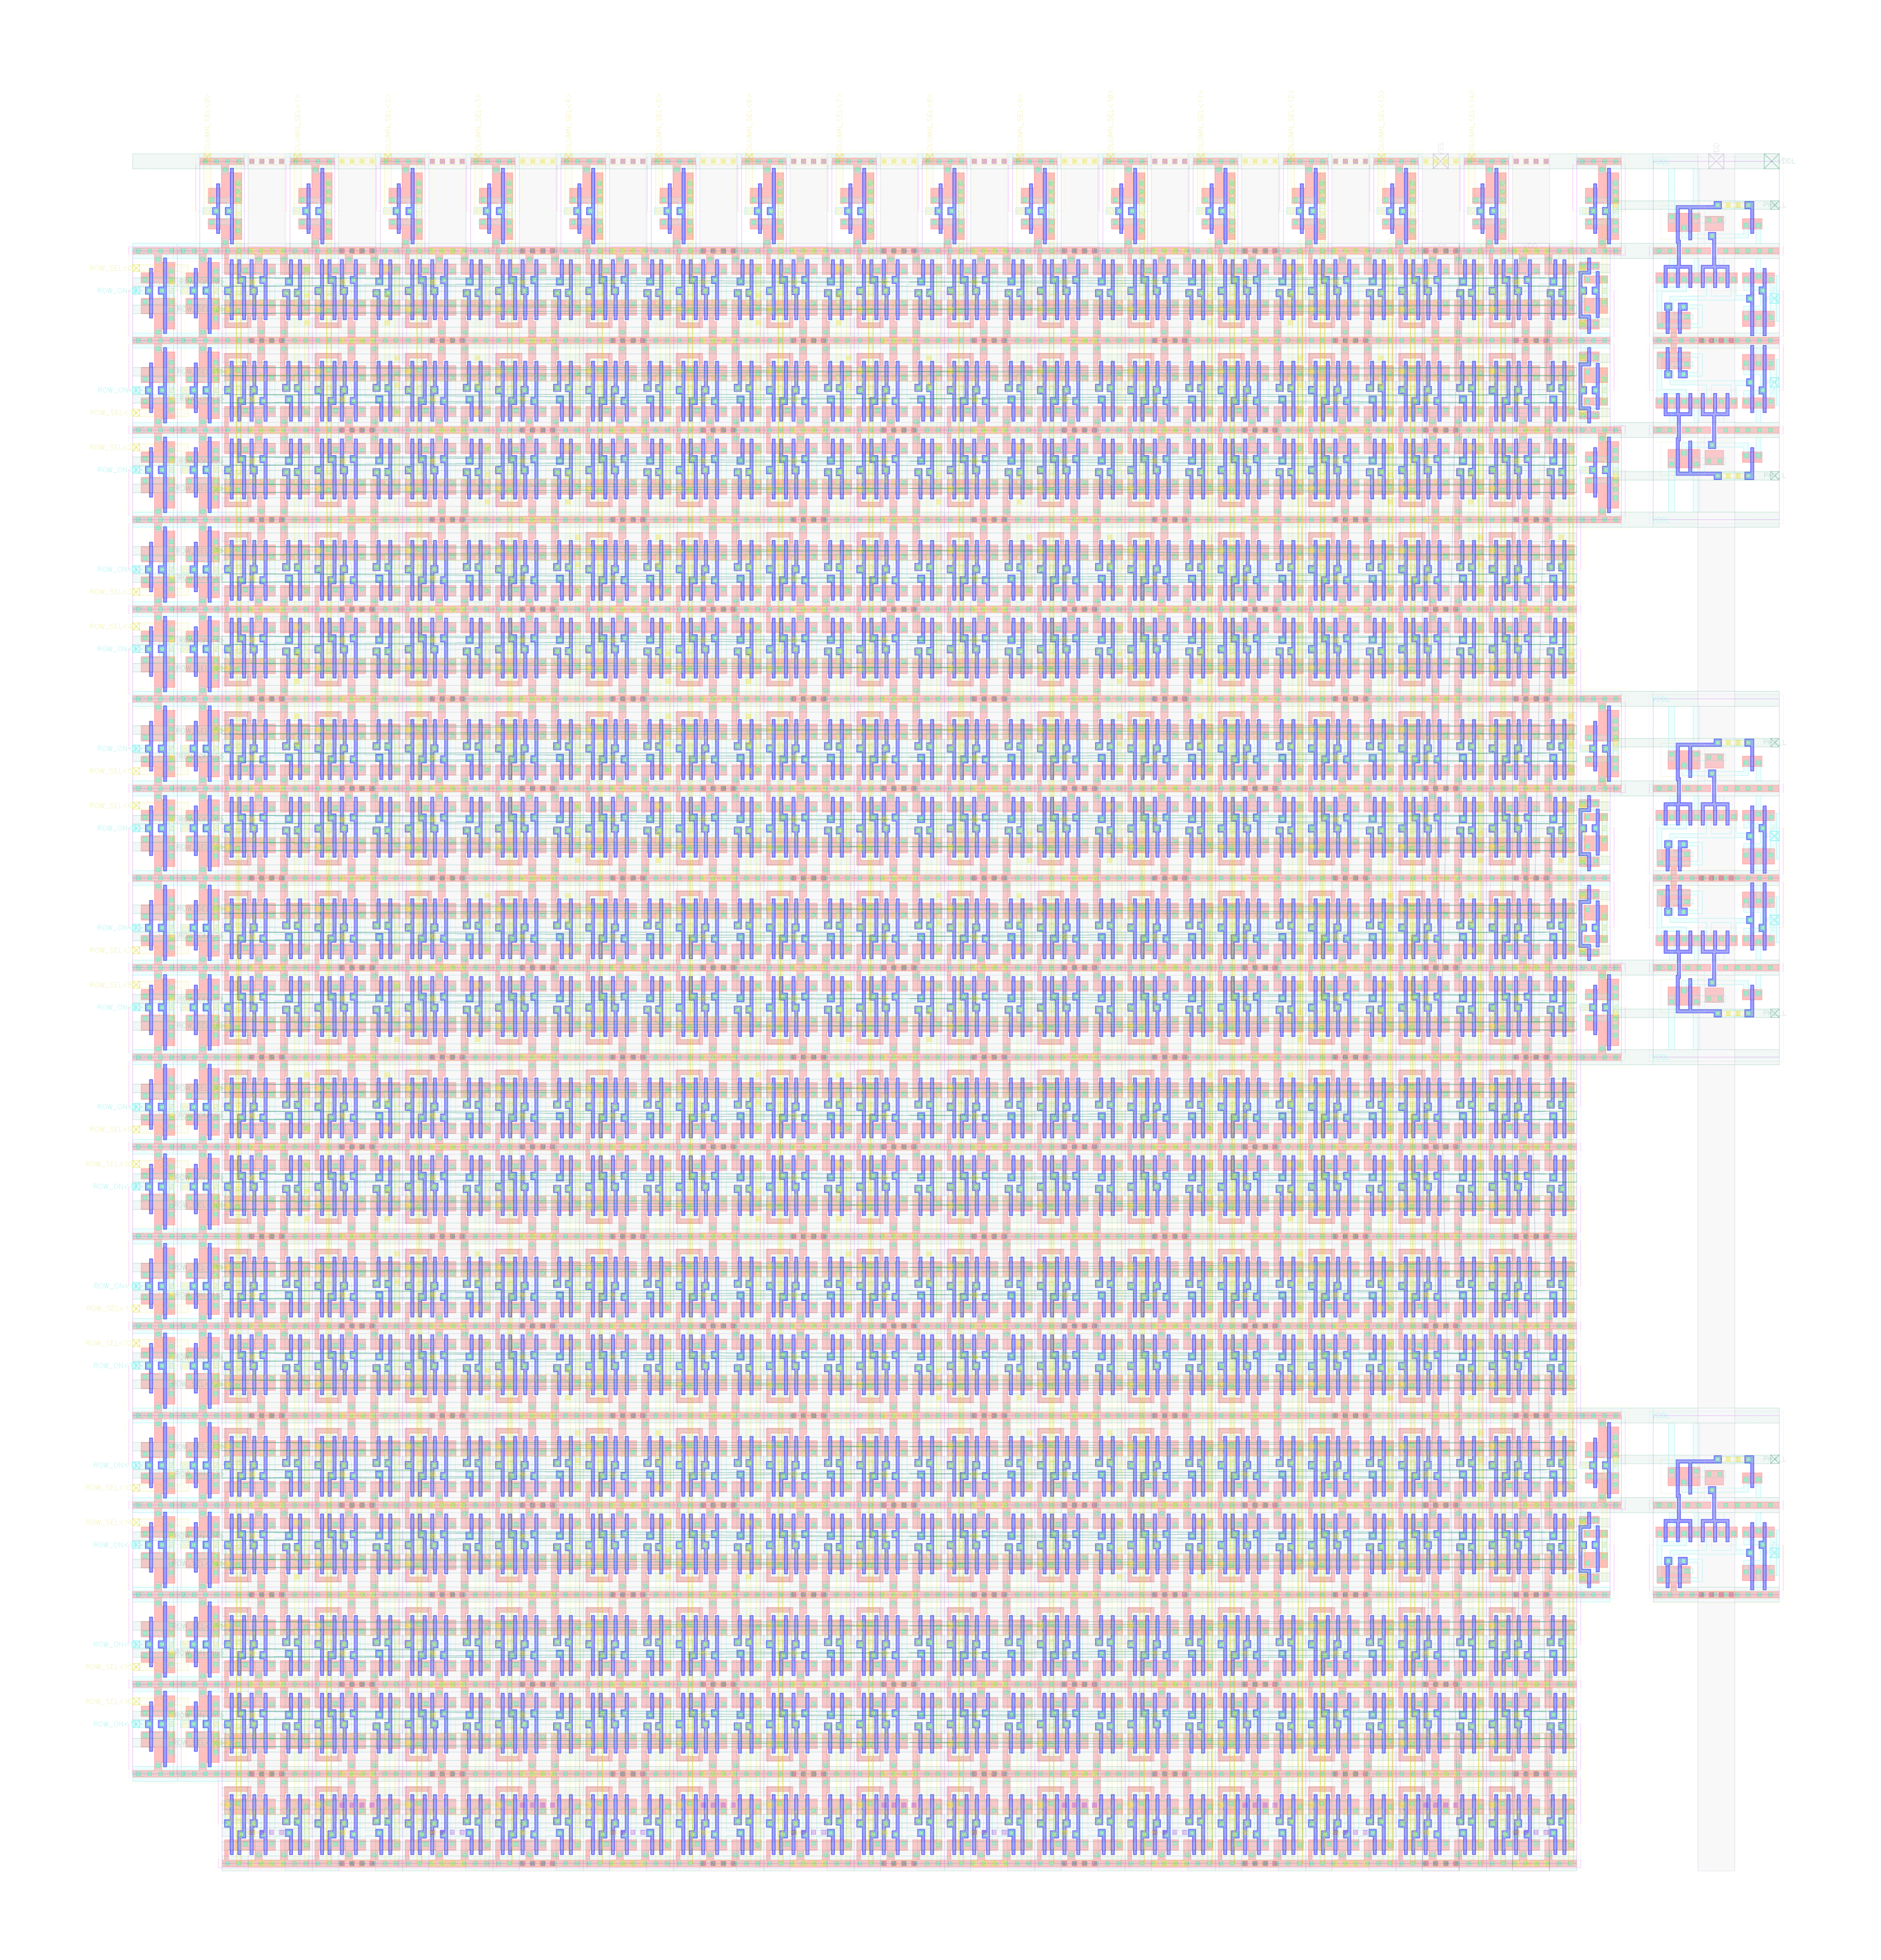
\includegraphics[scale=0.05]{slike/layout_dco5_hl_lh_130.png} };
        	\draw[<->] (-2.5,-2.45) -- (-2.5,2.03) node[midway, left=0.2, above=0.05, rotate=90] {\footnotesize 66,42\,\textmu m};
        	\draw[<->] (-1.97,-2.8) -- (1.8,-2.8) node[midway, right=0.1, below=0.02] {\footnotesize 55,8\,\textmu m};
        	\end{tikzpicture}
		\label{fig:compare_tech:layout:dco5_130}}
	\qquad
	\hspace{-0.55cm}
	\subfloat[\centering]{
	 	\begin{tikzpicture}
	 	% The image node
        	\node[inner sep=0] (layout_dco5_180_tech) { 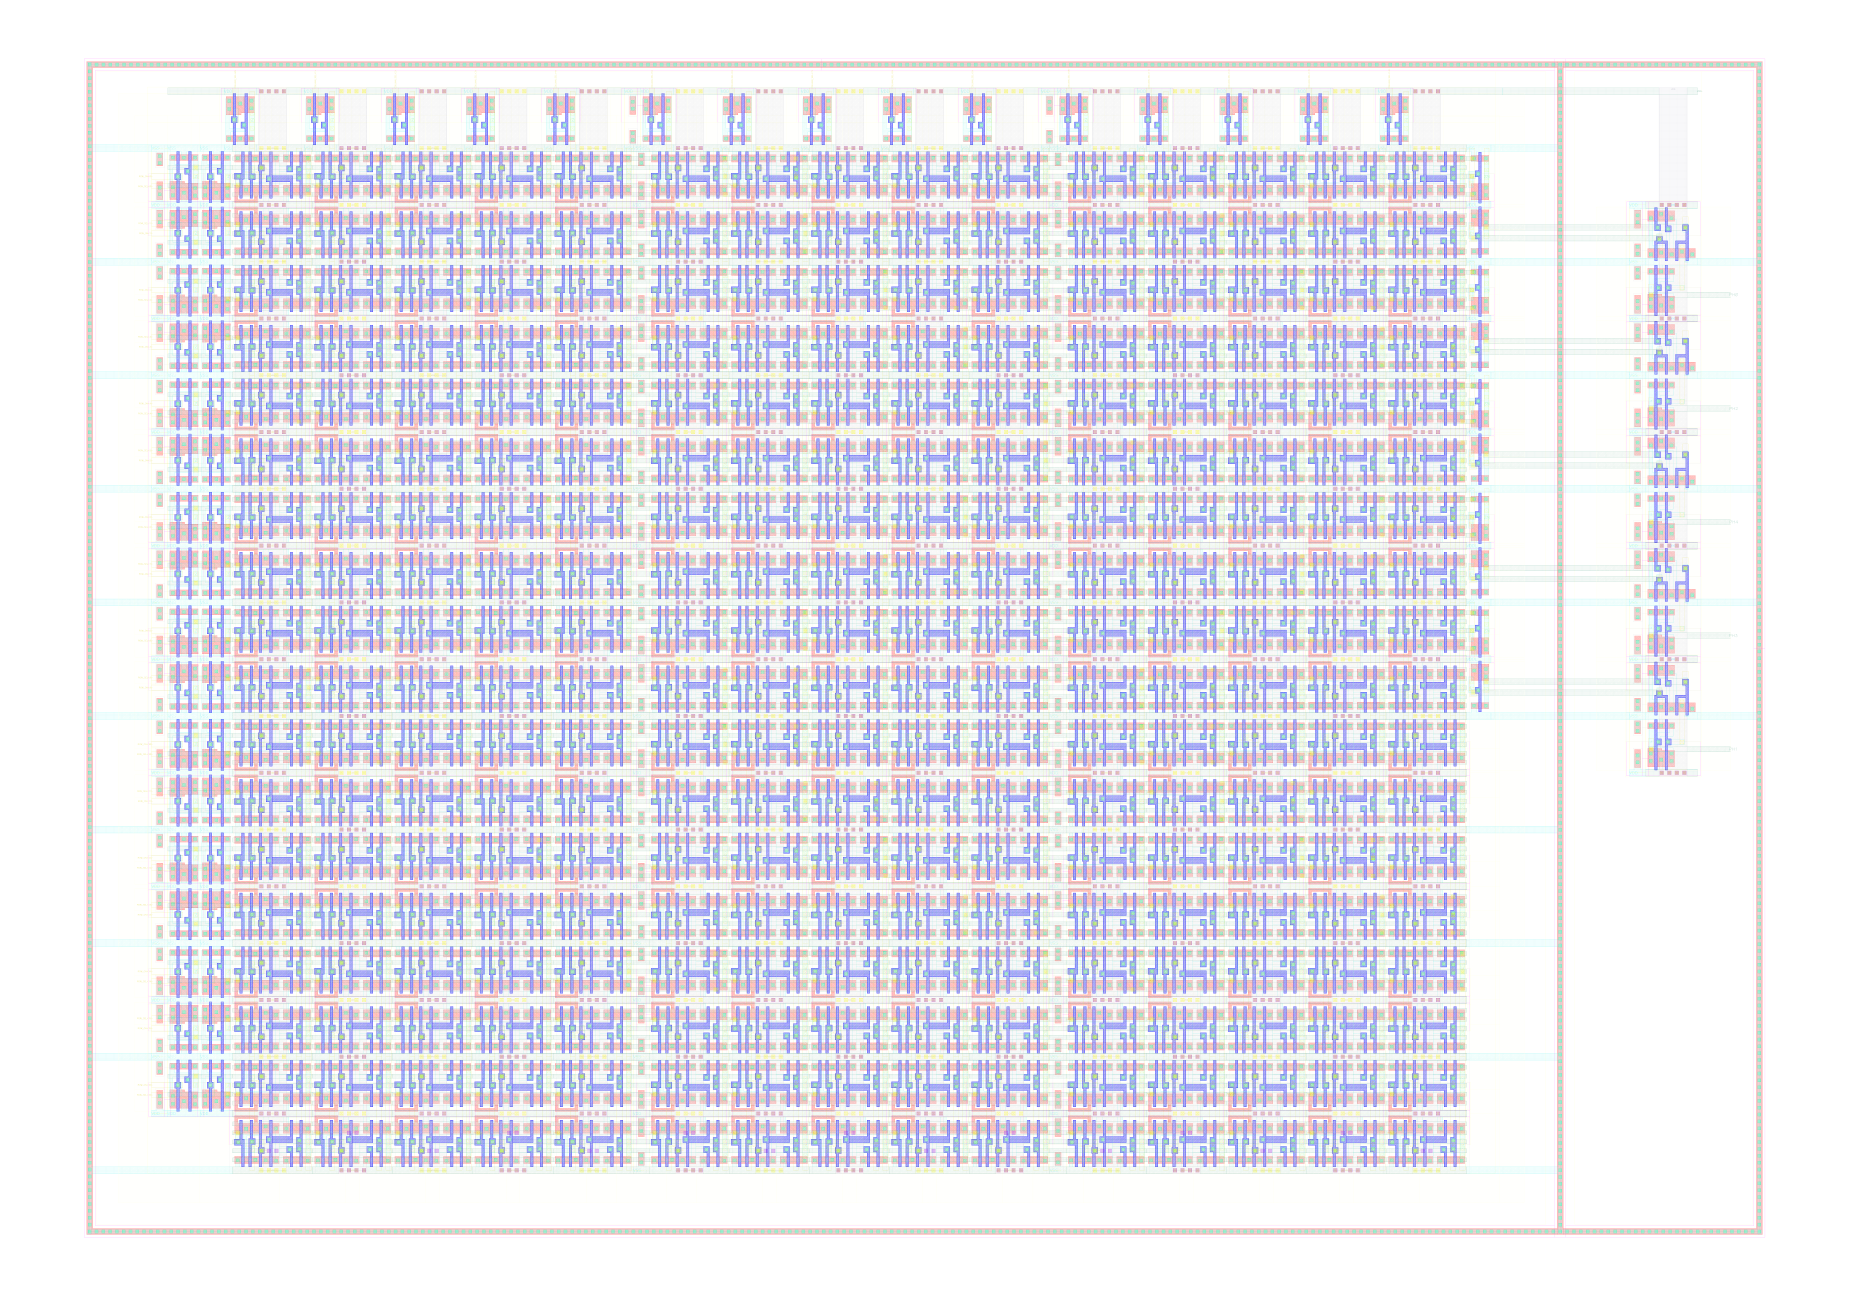
\includegraphics[width=8.8cm, height=6.18cm]{slike/layout_dco5_hl_lh_180.png} };
        	\draw[<->] (-4.3,-2.45) -- (-4.3,2.315) node[midway, left=0.2, above=0.05, rotate=90] {\footnotesize 70,557\,\textmu m};
        	\draw[<->] (-3.25,-3.1) -- (2.55,-3.1) node[midway, right=0.1, below=0.02] {\footnotesize 85,34\,\textmu m};
        	\end{tikzpicture}
		\label{fig:compare_tech:layout:dco5_180}}
	\caption{Лејаут \DCO-а пројектованог у TSMC (а) 130\,nm и (б) 180\,nm технологији.}
	\label{fig:compare_tech:layout:dco5}
\end{figure}
Скалирање транзистора обично долази са смањењем напона напајања, јер мањи транзистори могу радити на нижим напонима. То смањење напона смањује динамичку потрошњу, која је пропорционална квадрату напона напајања: 
\begin{equation}
	\label{eq:compare_tech:dyn_pwr}
	P_{dyn} = C_{L}V_{supply}^{2}f.
\end{equation}
Такође, смањење капацитивног оптерећења смањује динамичку потрошњу. У нашем случају извршене су симулације при раду на учестаности 640\,MHz у типичним условима рада са вриједностима $V_\text{DD}$=1,2\,V и $V_\text{DDL}$=1,1\,V за \DCO\ у 130\,nm и $V_\text{DD}$=1,8\,V и $V_\text{DDL}$=1,6\,V за \DCO\ у 180\,nm. Средње квадратне (RMS) вриједности потрошње струје и просјечна потрошња снаге на тим линијама напајања, за оба осцилатора, дати су у Tабели~\ref{tab:compare_tech:pwr}. Из резултата се види да је просјечна потрошња снаге мања за чак око 50\,\% (долази до изражаја квадратна зависност од напона напајања), a RMS вриједности струје за око 30\,\% за \DCO\ пројектован у 130\,nm. \par
\begin{table}[!ht]
	\caption{Поређење RMS вриједности потрошње струје и просјечне снаге \DCO-a пројектованих у 130\,nm и 180\,nm.}
	\label{tab:compare_tech:pwr}
	\centering
	\begin{tabular}{|c||c|c|}
		\hline
	         & 130\,nm & 180\,nm \\
		\specialrule{1.5pt}{0pt}{0pt}
		$\text{rms}(i_\text{DDL})$ & 2,185\,mA & 3,105\,mA \\
		\hline
		$\text{rms}(i_\text{DD})$ & 0,18\,mA & 0,27\,mA \\
		\hline
		Укупно rms($i$) & 2,365\,mA & 3,375\,mA \\
		\specialrule{1.5pt}{0pt}{0pt}
		$P_{avg}(V_\text{DDL})$ & 2,5\,mW & 5,0\,mW \\
		\hline
		$P_{avg}(V_\text{DD})$ & 0,22\,mW & 0,5\,mW \\
		\hline
		Укупно $P_{avg}$ & 2,72\,mW & 5,5\,mW \\
		\hline
	\end{tabular}
\end{table}
Додатна предност скалирања је што мањи транзистори могу радити на вишим учестаностима, што повећава укупне перформансе чипа. Разлог је то што скалирање транзистора доводи до смањења кашњења при пребацивању са 0 на 1 и обрнуто. Кашњење је сразмјерно отпорности и капацитивности гејта, а обје поменуте величине су директно пропорционалне димензијама гејта које се смањују скалирањем технологије. То значи да ће осцилатор у напреднијој технологији (у овом случају 130\,nm) бити у могућности да синтетише сигнал веће учестаности, за исти напон напајања. \tablename~\ref{tab:compare_tech:freq} приказује резултате симулација при различитим условима рада и вриједностима напона напајања. Подешавање параметара који одређују услове рада приказани су у Табели~\ref{tab:compare_tech:freq:cond}. \par 
\begin{table}[!ht]
	\caption{Подешавање услова рада за симулације опсега учестаности.}
	\label{tab:compare_tech:freq:cond}
	\centering
	\begin{tabular}{|c|c||c|c|c|c|}
		\hline
		Случај & Технологија & Процесни угао & Температура & $V_\text{DD}$ & $V_\text{DDL}$ \\
		\specialrule{1.5pt}{0pt}{0pt}
		Најспорији & 130\,nm & slow-slow & 125$^{\circ}\,C$ & 1,1\,V & 1,0\,V \\
		\hline
		Типични & 130\,nm & typical-typical & 40$^{\circ}\,C$ & 1,2\,V & 1,1\,V \\
		\hline
		Најбржи & 130\,nm & fast-fast & -40$^{\circ}$\,C & 1,3\,V & 1,2\,V \\
		\specialrule{1.5pt}{0pt}{0pt}
		Најспорији & 180\,nm & slow-slow & 125$^{\circ}$\,C & 1,6\,V & 1,4\,V \\
		\hline
		Типични & 180\,nm & typical-typical & 40$^{\circ}$\,C & 1,8\,V & 1,6\,V \\
		\hline
		Најбржи & 180\,nm & fast-fast & -40$^{\circ}$\,C & 2,0\,V & 1,8\,V \\
		\hline
	\end{tabular}
\end{table}
\begin{table}[!ht]
	\caption{Поређење опсега учестаности при различитим условима рада за \DCO\ пројектован у 130\,nm и 180\,nm.}
	\label{tab:compare_tech:freq}
	\centering
	\begin{tabular}{|c|c||c|c|}
		\hline
		Случај & Технологија & $f_\text{min}$ & $f_\text{max}$ \\
		\specialrule{1.5pt}{0pt}{0pt}
		Најспорији & 130\,nm & 27,2\,MHz & 502\,MHz \\
		\hline
		Типични & 130\,nm & 42\,MHz & 764\,MHz \\
		\hline
		Најбржи & 130\,nm & 63,3\,MHz & 1,146\,GHz \\
		\specialrule{1.5pt}{0pt}{0pt}
		Најспорији & 180\,nm & 23,06\,MHz & 421,4\,MHz \\
		\hline
		Типични & 180\,nm & 40\,MHz & 726\,MHz \\
		\hline
		Најбржи & 180\,nm & 64,43\,MHz & 1,168\,GHz \\
		\hline
	\end{tabular}
\end{table}
Из резултата се види да се скалирањем технологије значајно може смањити напон напајања да би се добио жељени опсег учестаности, што наравно значи да се уз много мању потрошњу постижу сличне, или чак боље, перформансе у раду \DCO-а. \par
\subsection{Начин и утицај коришћења дубоке јаме N типа у аналогном пројектовању \DCO-а}
Дитално контролисани осцилатор пројектован у 180\,nm TSMC технологији, поред стандардних јама \engl{Well} P и N типа, посједује додатну тзв. дубоку јаму N типа \engl[DNW]{Deep N-Well}. Да би се показало чему она служи, потребно је анализирати појаве које се дешавају у слојевима у које су сами транзистори уроњени. Приликом рада транзистора појављује се шум у супстрату који се дешава због убризгавања наелектрисања у супстрат и јаме. Тај проблем се рјешава употребом n$+$ и p$+$ спојева \engl{Tap} повезаних редом на $V_\text{DD}$ и $V_\text{SS}$, за PMOS и NMOS транзисторе, респективно (\figurename~\ref{fig:dnw:typical}). Додатни проблем је што постоји капацитивно спрезање између N јаме и P супстрата, што значи да више шума долази до извора. У дигиталним колима то обично није проблем због прилично високе отпорности логичких кола на шум. Међутим, у аналогном пројектовању, шум може бити озбиљан проблем па се користе различите технике за његово сузбијање као што су додавање заштитних прстенова \engl{Guard Ring} или коришћење одвојеног напајања за спојеве у супстрату и јамама. Треба поменути да заштитни прстенови не могу спријечити појаву шума дубоко у супстрату~\cite{DNW:aspencore}. Други проблем је што NMOS транзистори обично нису изоловани од супстрата. У основној CMOS изради, NMOS транзистор је уроњен у P супстрат повезан на масу, док је PMOS уроњен у N јаму \engl{N-Well} повезану на напајање, као што је приказано на Слици~\ref{fig:dnw:typical}. \par
\begin{figure}[!ht]
    \centering
    \vspace{-0.1cm}
    \begin{tikzpicture}

    % P substrate
    \node[draw, rectangle, fill=red!20, minimum height=2.5cm, minimum width=15cm, inner sep=0] (psub) at (0,-1.25) {};

    % N well
    \node[draw, rectangle, fill=yellow!30, minimum height=1.3cm, minimum width=6cm, inner sep=0] (nwell) at (-4,-0.65) {};

    % PMOS Source/Drain (P+ diffusion)
    \node[draw, rectangle, fill=red!55, minimum height=0.5cm, minimum width=1cm, inner sep=0] (psource) at (-6.0,-0.25) {\footnotesize p\,\scriptsize $+$};
    \node[draw, rectangle, fill=red!55, minimum height=0.5cm, minimum width=1cm, inner sep=0] (pdrain) at (-4.0,-0.25) {\footnotesize p\,\scriptsize $+$};

    % NMOS Source/Drain (N+ diffusion)
    \node[draw, rectangle, fill=yellow, minimum height=0.5cm, minimum width=1cm, inner sep=0] (nsource) at (4.0,-0.25) {\footnotesize n\,\scriptsize $+$};
    \node[draw, rectangle, fill=yellow, minimum height=0.5cm, minimum width=1cm, inner sep=0] (ndrain) at (6.0,-0.25) {\footnotesize n\,\scriptsize $+$};

    % Gate oxide and Gate for PMOS and NMOS
    \node[draw, rectangle, fill=gray!40, minimum height=0.1cm, minimum width=1.6cm, inner sep=0] (pgray) at (-5.0,0.05) {};
    \node[draw, rectangle, fill=gray!40, minimum height=0.1cm, minimum width=1.6cm, inner sep=0] (ngray) at (5.0,0.05) {};
    \node[draw, rectangle, fill=blue!30, minimum height=0.4cm, minimum width=1.4cm, inner sep=0] (pgate) at (-5.0,0.3) {};
    \node[draw, rectangle, fill=blue!30, minimum height=0.4cm, minimum width=1.4cm, inner sep=0] (ngate) at (5.0,0.3) {};

    % Taps and Substrate Contacts
    % \node[draw, rectangle, fill=yellow!60, minimum height=0.5cm, minimum width=1cm, inner sep=0] (ntap) at (-2,-0.25) {\footnotesize n\scriptsize $+$\,\footnotesize tap};
    % \node[draw, rectangle, fill=red!55, minimum height=0.5cm, minimum width=1cm, inner sep=0] (ptap) at (2,-0.25) {\footnotesize p\scriptsize $+$\,\footnotesize tap};
    
    % Taps and Substrate Contacts
    \node[draw, rectangle, fill=yellow, minimum height=0.5cm, minimum width=1cm, inner sep=0] (ntap) at (-2,-0.25) {\footnotesize n\scriptsize $+$};
    \node[draw, rectangle, fill=red!55, minimum height=0.5cm, minimum width=1cm, inner sep=0] (ptap) at (2,-0.25) {\footnotesize p\scriptsize $+$};


    \draw (ngate.north) --++ (0,0.5) node[draw, circle, minimum size=0.13cm, inner sep=0, fill=white](ngatecirc){} ++ (0,0.1) node[anchor=south]{\footnotesize G};
    \draw (nsource.north) --++ (0,1) node[draw, circle, minimum size=0.13cm, inner sep=0, fill=white](nsourcecirc){} ++ (0,0.1) node[anchor=south]{\footnotesize S};
    \draw (ndrain.north) --++ (0,1) node[draw, circle, minimum size=0.13cm, inner sep=0, fill=white](ndraincirc){} ++ (0,0.1) node[anchor=south]{\footnotesize D};
    \draw (ntap.north) --++ (0,1) node[draw, circle, minimum size=0.13cm, inner sep=0, fill=white](ntapcirc){} ++ (0,0.05) node[anchor=south]{\footnotesize B ($V_\text{DD}$)};

    \draw (pgate.north) --++ (0,0.5) node[draw, circle, minimum size=0.13cm, inner sep=0, fill=white](pgatecirc){} ++ (0,0.1) node[anchor=south]{\footnotesize G};
    \draw (psource.north) --++ (0,1) node[draw, circle, minimum size=0.13cm, inner sep=0, fill=white](psourcecirc){} ++ (0,0.1) node[anchor=south]{\footnotesize S};
    \draw (pdrain.north) --++ (0,1) node[draw, circle, minimum size=0.13cm, inner sep=0, fill=white](pdraincirc){} ++ (0,0.1) node[anchor=south]{\footnotesize D};
    \draw (ptap.north) --++ (0,1) node[draw, circle, minimum size=0.13cm, inner sep=0, fill=white](ptapcirc){} ++ (0,0.05) node[anchor=south]{\footnotesize B ($V_\text{SS}$)};

    \draw[decoration={brace},decorate] (-7,1.7) -- node[above=1pt] {\footnotesize PMOS} (-1,1.7);
    \draw[decoration={brace},decorate] (1,1.7) -- node[above=1pt] {\footnotesize NMOS} (7,1.7);
    % Labels
    \draw (nwell.south west) ++ (0.08,0.08) node[anchor=south west] {\footnotesize N-Well};
    \draw (psub.south) ++ (0.1,0.1) node[anchor=south] {\footnotesize P-Substrate};

    \draw (psub.south) node[ground] (gnd) {};

    \end{tikzpicture}
    \vspace{-0.1cm}
    \caption{Попречни пресјек типичног CMOS инвертора.}
    \label{fig:dnw:typical}
\end{figure}

Изолација NMOS транзистора се може постићи коришћењем поменуте дубоке јаме N типа. Она се формира уметањем високоенергетске јонске имплантације непосредно прије формирања стандардне јаме N типа~\cite{DNW:1503847}. Повезивање дубоке јаме N типа врши се преко стандардне јаме N типа која је окружује и повезана је на напајање, $V_\text{DD}$. Тако се, стварањем изоловане јаме P типа \engl{P-Well}, изолује NMOS транзистор. Како додатном изолацијом глобални P супстрат остаје без p$+$ споја који је неопходан да се појавом шума у супстрату не наруше перформансе уређаја, додаје се заштитни прстен који се повезује на $V_\text{SS}$. \figurename~\ref{fig:dnw:dnw_cmos} приказује начин изолације NMOS транзистора преко дубоке јаме N типа уз додати заштитни прстен. \par
\begin{figure}[!ht]
    \centering
    %\vspace{0.2cm}
    \vspace{-0.1cm}
    %\resizebox{10cm}{2cm}{%
    \scalebox{0.78}{
    \begin{tikzpicture}

    % P substrate
    \node[draw, rectangle, fill=red!20, minimum height=3.5cm, minimum width=20.1cm, inner sep=0] (psub) at (2.55,-1.75) {};

    % N well
    \node[draw, rectangle, fill=yellow!30, minimum height=1.3cm, minimum width=6cm, inner sep=0] (nwell) at (-4,-0.65) {};
    
    % Left N well above DNW
    \node[draw, rectangle, fill=yellow!30, minimum height=1.3cm, minimum width=1.6cm, inner sep=0] (nwelldnwleft) at (2,-0.65) {};
    % Right N well above DNW
    \node[draw, rectangle, fill=yellow!30, minimum height=1.3cm, minimum width=1.6cm, inner sep=0] (nwelldnwright) at (10,-0.65) {};
    
    % DNW Rectangle
    \node[draw, rectangle, fill=YellowGreen!30, minimum height=1.3cm, minimum width=8.4cm, inner sep=0] (dnw) at (6,-1.95) {};

    % PMOS Source/Drain (P+ diffusion)
    \node[draw, rectangle, fill=red!55, minimum height=0.5cm, minimum width=1cm, inner sep=0] (psource) at (-6.0,-0.25) {\footnotesize p\,\scriptsize $+$};
    \node[draw, rectangle, fill=red!55, minimum height=0.5cm, minimum width=1cm, inner sep=0] (pdrain) at (-4.0,-0.25) {\footnotesize p\,\scriptsize $+$};

    % Guard ring - left tap
    \node[draw, rectangle, fill=red!55, minimum height=0.5cm, minimum width=1cm, inner sep=0] (grleft) at (0.4,-0.25) {\footnotesize p\,\scriptsize $+$};
    % DNW - left tap
    \node[draw, rectangle, fill=yellow, minimum height=0.5cm, minimum width=1cm, inner sep=0] (dnwleft) at (2,-0.25) {\footnotesize n\,\scriptsize $+$};
    
    % Guard ring - right tap
    \node[draw, rectangle, fill=red!55, minimum height=0.5cm, minimum width=1cm, inner sep=0] (grright) at (11.6,-0.25) {\footnotesize p\,\scriptsize $+$};
    % DNW - rignt tap
    \node[draw, rectangle, fill=yellow, minimum height=0.5cm, minimum width=1cm, inner sep=0] (dnwright) at (10,-0.25) {\footnotesize n\,\scriptsize $+$};

    % NMOS Source/Drain (N+ diffusion)
    \node[draw, rectangle, fill=yellow, minimum height=0.5cm, minimum width=1cm, inner sep=0] (nsource) at (6.0,-0.25) {\footnotesize n\,\scriptsize $+$};
    \node[draw, rectangle, fill=yellow, minimum height=0.5cm, minimum width=1cm, inner sep=0] (ndrain) at (8.0,-0.25) {\footnotesize n\,\scriptsize $+$};

    % Gate oxide and Gate for PMOS and NMOS
    \node[draw, rectangle, fill=gray!40, minimum height=0.1cm, minimum width=1.6cm, inner sep=0] (pgray) at (-5.0,0.05) {};
    \node[draw, rectangle, fill=gray!40, minimum height=0.1cm, minimum width=1.6cm, inner sep=0] (ngray) at (7.0,0.05) {};
    \node[draw, rectangle, fill=blue!30, minimum height=0.4cm, minimum width=1.4cm, inner sep=0] (pgate) at (-5.0,0.3) {};
    \node[draw, rectangle, fill=blue!30, minimum height=0.4cm, minimum width=1.4cm, inner sep=0] (ngate) at (7.0,0.3) {};

    % Taps and Substrate Contacts
    % \node[draw, rectangle, fill=yellow, minimum height=0.5cm, minimum width=1cm, inner sep=0] (ntap) at (-2,-0.25) {\footnotesize n\scriptsize $+$\,\footnotesize tap};
    % \node[draw, rectangle, fill=red!55, minimum height=0.5cm, minimum width=1cm, inner sep=0] (ptap) at (4,-0.25) {\footnotesize p\scriptsize $+$\,\footnotesize tap};

    % Taps and Substrate Contacts
    \node[draw, rectangle, fill=yellow, minimum height=0.5cm, minimum width=1cm, inner sep=0] (ntap) at (-2,-0.25) {\footnotesize n\scriptsize $+$};
    \node[draw, rectangle, fill=red!55, minimum height=0.5cm, minimum width=1cm, inner sep=0] (ptap) at (4,-0.25) {\footnotesize p\scriptsize $+$};

    % NMOS contacts
    \draw (ngate.north) --++ (0,0.5) node[draw, circle, minimum size=0.13cm, inner sep=0, fill=white](ngatecirc){} ++ (0,0.1) node[anchor=south]{\footnotesize G};
    \draw (nsource.north) --++ (0,1) node[draw, circle, minimum size=0.13cm, inner sep=0, fill=white](nsourcecirc){} ++ (0,0.1) node[anchor=south]{\footnotesize S};
    \draw (ndrain.north) --++ (0,1) node[draw, circle, minimum size=0.13cm, inner sep=0, fill=white](ndraincirc){} ++ (0,0.1) node[anchor=south]{\footnotesize D};
    \draw (ntap.north) --++ (0,1) node[draw, circle, minimum size=0.13cm, inner sep=0, fill=white](ntapcirc){} ++ (0,0.05) node[anchor=south]{\footnotesize B ($V_\text{DD}$)};

    % PMOS contacts
    \draw (pgate.north) --++ (0,0.5) node[draw, circle, minimum size=0.13cm, inner sep=0, fill=white](pgatecirc){} ++ (0,0.1) node[anchor=south]{\footnotesize G};
    \draw (psource.north) --++ (0,1) node[draw, circle, minimum size=0.13cm, inner sep=0, fill=white](psourcecirc){} ++ (0,0.1) node[anchor=south]{\footnotesize S};
    \draw (pdrain.north) --++ (0,1) node[draw, circle, minimum size=0.13cm, inner sep=0, fill=white](pdraincirc){} ++ (0,0.1) node[anchor=south]{\footnotesize D};
    \draw (ptap.north) --++ (0,1) node[draw, circle, minimum size=0.13cm, inner sep=0, fill=white](ptapcirc){} ++ (0,0.05) node[anchor=south]{\footnotesize B ($V_\text{SS}$)};

    % Guard Ring contacts
    \draw (grleft.north) --++ (0,1) node[draw, circle, minimum size=0.13cm, inner sep=0, fill=white](grleftcirc){} ++ (0,0.1) node[anchor=south]{\footnotesize $V_\text{SS}$};
    \draw (grright.north) --++ (0,1) node[draw, circle, minimum size=0.13cm, inner sep=0, fill=white](grrightcirc){} ++ (0,0.1) node[anchor=south]{\footnotesize $V_\text{SS}$};

    % Contacts for taps in N-well above DNW
    \draw (dnwleft.north) --++ (0,1) node[draw, circle, minimum size=0.13cm, inner sep=0, fill=white](dnwleftcirc){} ++ (0,0.1) node[anchor=south]{\footnotesize $V_\text{DD}$};
    \draw (dnwright.north) --++ (0,1) node[draw, circle, minimum size=0.13cm, inner sep=0, fill=white](dnwrightcirc){} ++ (0,0.1) node[anchor=south]{\footnotesize $V_\text{DD}$};

    % Curly braces
    \draw[decoration={brace},decorate] (-7,1.7) -- node[above=1pt] {\footnotesize PMOS} (-1,1.7);
    \draw[decoration={brace},decorate] (3,1.7) -- node[above=1pt] {\footnotesize NMOS} (9,1.7);
    
    % Labels
    \draw (nwell.south) ++ (0,0.1) node[anchor=south] {\footnotesize N-Well};
    \draw (psub.south) ++ (0,0.1) node[anchor=south] {\footnotesize P-Substrate};
    \draw (nwelldnwleft.south) ++ (0,0.1) node[anchor=south] {\footnotesize N-Well};
    \draw (nwelldnwright.south) ++ (0,0.1) node[anchor=south] {\footnotesize N-Well};
    \draw (dnw.south) ++ (0,0.1) node[anchor=south] {\footnotesize Deep N-Well};
    \draw (dnw.north) ++ (0,0.1) node[anchor=south] {\footnotesize P-Well};

    % Substrate ground
    \draw (psub.south) node[ground] (gnd) {};

    \end{tikzpicture}
    }
    %\vspace{0.5cm}
    \caption{Попречни пресјек PMOS и NMOS транзистора, гдје је NMOS транзистор изолован дубоком јамом N типа \engl{Deep N-Well} са додатим заштитним прстеном повезаним на $V_\text{SS}$.}
    \label{fig:dnw:dnw_cmos}
\end{figure}

Како NMOS и PMOS транзистори обично иду у пару приликом CMOS пројектовања, да би се боље искористио простор тј. смањила површина крајњег лејаута, за повезивање дубоке јаме N типа се може искористити стандардна јама N типа коју користи PMOS транзистор, а заштитни прстен се помјера да обухвати читав дизајн, што је приказано на Слици~\ref{fig:dnw:dnw_cmos_compact}. У конкретном дизајну \DCO-a, са Слике~\ref{fig:compare_tech:layout:dco5_180} се може уочити заштитни прстен који обухвата читав \DCO. \par
\begin{figure}[!ht]
    \centering
    \vspace{-0.1cm}
    %\resizebox{10cm}{2cm}{%
    \scalebox{0.9}{
    \begin{tikzpicture}

    % P substrate
    \node[draw, rectangle, fill=red!20, minimum height=3.5cm, minimum width=17.5cm, inner sep=0] (psub) at (3.855,-1.75) {};

    % N well
    \node[draw, rectangle, fill=yellow!30, minimum height=1.3cm, minimum width=5.8cm, inner sep=0] (nwell) at (-0.1,-0.65) {};
    
    % Right N well above DNW
    \node[draw, rectangle, fill=yellow!30, minimum height=1.3cm, minimum width=1.6cm, inner sep=0] (nwelldnwright) at (10,-0.65) {};
    
    % DNW Rectangle
    \node[draw, rectangle, fill=YellowGreen!30, minimum height=1.3cm, minimum width=8.4cm, inner sep=0] (dnw) at (6,-1.95) {};

    % PMOS Source/Drain (P+ diffusion)
    \node[draw, rectangle, fill=red!55, minimum height=0.5cm, minimum width=1cm, inner sep=0] (psource) at (-2.0,-0.25) {\footnotesize p\,\scriptsize $+$};
    \node[draw, rectangle, fill=red!55, minimum height=0.5cm, minimum width=1cm, inner sep=0] (pdrain) at (0.0,-0.25) {\footnotesize p\,\scriptsize $+$};

    % Guard ring - left tap
    \node[draw, rectangle, fill=red!55, minimum height=0.5cm, minimum width=1cm, inner sep=0] (grleft) at (-3.8,-0.25) {\footnotesize p\,\scriptsize $+$};
    
    % Guard ring - right tap
    \node[draw, rectangle, fill=red!55, minimum height=0.5cm, minimum width=1cm, inner sep=0] (grright) at (11.6,-0.25) {\footnotesize p\,\scriptsize $+$};
    % DNW - rignt tap
    \node[draw, rectangle, fill=yellow, minimum height=0.5cm, minimum width=1cm, inner sep=0] (dnwright) at (10,-0.25) {\footnotesize n\,\scriptsize $+$};

    % NMOS Source/Drain (N+ diffusion)
    \node[draw, rectangle, fill=yellow, minimum height=0.5cm, minimum width=1cm, inner sep=0] (nsource) at (6.0,-0.25) {\footnotesize n\,\scriptsize $+$};
    \node[draw, rectangle, fill=yellow, minimum height=0.5cm, minimum width=1cm, inner sep=0] (ndrain) at (8.0,-0.25) {\footnotesize n\,\scriptsize $+$};

    % Gate oxide and Gate for PMOS and NMOS
    \node[draw, rectangle, fill=gray!40, minimum height=0.1cm, minimum width=1.6cm, inner sep=0] (pgray) at (-1.0,0.05) {};
    \node[draw, rectangle, fill=gray!40, minimum height=0.1cm, minimum width=1.6cm, inner sep=0] (ngray) at (7.0,0.05) {};
    \node[draw, rectangle, fill=blue!30, minimum height=0.4cm, minimum width=1.4cm, inner sep=0] (pgate) at (-1.0,0.3) {};
    \node[draw, rectangle, fill=blue!30, minimum height=0.4cm, minimum width=1.4cm, inner sep=0] (ngate) at (7.0,0.3) {};

    % Taps and Substrate Contacts
    % \node[draw, rectangle, fill=yellow, minimum height=0.5cm, minimum width=1cm, inner sep=0] (ntap) at (2,-0.25) {\footnotesize n\scriptsize $+$\,\footnotesize tap};
    % \node[draw, rectangle, fill=red!55, minimum height=0.5cm, minimum width=1cm, inner sep=0] (ptap) at (4,-0.25) {\footnotesize p\scriptsize $+$\,\footnotesize tap};

    % Taps and Substrate Contacts
    \node[draw, rectangle, fill=yellow, minimum height=0.5cm, minimum width=1cm, inner sep=0] (ntap) at (2,-0.25) {\footnotesize n\scriptsize $+$};
    \node[draw, rectangle, fill=red!55, minimum height=0.5cm, minimum width=1cm, inner sep=0] (ptap) at (4,-0.25) {\footnotesize p\scriptsize $+$};

    % NMOS contacts
    \draw (ngate.north) --++ (0,0.5) node[draw, circle, minimum size=0.13cm, inner sep=0, fill=white](ngatecirc){} ++ (0,0.1) node[anchor=south]{\footnotesize G};
    \draw (nsource.north) --++ (0,1) node[draw, circle, minimum size=0.13cm, inner sep=0, fill=white](nsourcecirc){} ++ (0,0.1) node[anchor=south]{\footnotesize S};
    \draw (ndrain.north) --++ (0,1) node[draw, circle, minimum size=0.13cm, inner sep=0, fill=white](ndraincirc){} ++ (0,0.1) node[anchor=south]{\footnotesize D};
    \draw (ntap.north) --++ (0,1) node[draw, circle, minimum size=0.13cm, inner sep=0, fill=white](ntapcirc){} ++ (0,0.05) node[anchor=south]{\footnotesize B ($V_\text{DD}$)};

    % PMOS contacts
    \draw (pgate.north) --++ (0,0.5) node[draw, circle, minimum size=0.13cm, inner sep=0, fill=white](pgatecirc){} ++ (0,0.1) node[anchor=south]{\footnotesize G};
    \draw (psource.north) --++ (0,1) node[draw, circle, minimum size=0.13cm, inner sep=0, fill=white](psourcecirc){} ++ (0,0.1) node[anchor=south]{\footnotesize S};
    \draw (pdrain.north) --++ (0,1) node[draw, circle, minimum size=0.13cm, inner sep=0, fill=white](pdraincirc){} ++ (0,0.1) node[anchor=south]{\footnotesize D};
    \draw (ptap.north) --++ (0,1) node[draw, circle, minimum size=0.13cm, inner sep=0, fill=white](ptapcirc){} ++ (0,0.05) node[anchor=south]{\footnotesize B ($V_\text{SS}$)};

    % Guard Ring contacts
    \draw (grleft.north) --++ (0,1) node[draw, circle, minimum size=0.13cm, inner sep=0, fill=white](grleftcirc){} ++ (0,0.1) node[anchor=south]{\footnotesize $V_\text{SS}$};
    \draw (grright.north) --++ (0,1) node[draw, circle, minimum size=0.13cm, inner sep=0, fill=white](grrightcirc){} ++ (0,0.1) node[anchor=south]{\footnotesize $V_\text{SS}$};

    % Contacts for taps in N-well above DNW
    \draw (dnwright.north) --++ (0,1) node[draw, circle, minimum size=0.13cm, inner sep=0, fill=white](dnwrightcirc){} ++ (0,0.1) node[anchor=south]{\footnotesize $V_\text{DD}$};

    % Curly braces
    \draw[decoration={brace},decorate] (-3,1.7) -- node[above=1pt] {\footnotesize PMOS} (2.8,1.7);
    \draw[decoration={brace},decorate] (3,1.7) -- node[above=1pt] {\footnotesize NMOS} (9,1.7);
    
    % Labels
    \draw (nwell.south) ++ (0,0.1) node[anchor=south] {\footnotesize N-Well};
    \draw (psub.south) ++ (0,0.1) node[anchor=south] {\footnotesize P-Substrate};
    \draw (nwelldnwright.south) ++ (0,0.1) node[anchor=south] {\footnotesize N-Well};
    \draw (dnw.south) ++ (0,0.1) node[anchor=south] {\footnotesize Deep N-Well};
    \draw (dnw.north) ++ (0,0.1) node[anchor=south] {\footnotesize P-Well};

    % Substrate ground
    \draw (psub.south) node[ground] (gnd) {};

    \end{tikzpicture}
    }
    %\vspace{0.5cm}
    \caption{Попречни пресјек просторно ефикаснијег лејаута PMOS и изолованог NMOS транзистора.}
    \label{fig:dnw:dnw_cmos_compact}
    \vspace{-0.1cm}
\end{figure}

Дакле, дубока јама N типа има улогу у смањењу шума у супстрату и омогућава потпуно изоловање NMOS транзистора, који, теоретски, након тога могу бити на потенцијалу различитом од масе~\cite{DNW:aspencore}. Како додавање дубоке јаме N типа изискује и додавање заштитног прстена, површина коју заузима дизајн се повећава, тако да то може бити недостатак овог приступа ако су захтјеви за површином строги. Углавном то није случај јер су захтјеви за перформансама обично битнији тако да је цијена која се плаћа у површини занемарљива у односу на предности које има изолација NMOS транзистора у погледу смањења шума у супстрату.

\section{Закључак} \label{Conclusion}
У овом раду представљена је синтетизабилна дигитална фреквенцијски затворена петља са једноставном али ефикасном архитектуром. Дигитално контролисан осцилатор са прстенастом структуром, састављен од тростатичких инвертора омогућава достизање пристојне резолуције учестаности и одговарајућих радних перформанси. Додатне предности су му и једноставно управљање, прилагодљивост и једноставна поновна употреба. Представљена су два управљачка режима \FLL-а: двостепени регулатор и \PID\ регулатор. За сваки од њих је детаљно објашњен начин рада и вјеродостојно су приказане разлике у одзиву система у различитим управљачким режимима. Детаљно је објашњена размјена података између различитих домена такта, као и методе заштите од метастабилности. \par
\FLL\ из овог рада је имплементиран у SystemVerilog језику за опис хардвера. У зависности од технолошке библиотеке може бити направљен коришћењем само библиотеке стандардних ћелија без преуређивања у току дигиталног пројектовања. Обрађени \FLL\ је послат на фабрикацију у 130\,nm CMOS технологији. \par
Ради додатне верификације направљен је и демонстриран софтверски модел рада читавог \FLL-a написан у Пајтон програмском језику. Поред саме демонстрације рада, захваљујући параметрима које прима, помоћу модела се на бржи и једноставнији начин могу предвидјети исправне вриједности константи које се задају систему (нпр. константе \PID\ регулатора), што значајно убрзава пројектовање.\par
У сврху приказа утицаја скалирања технологије на рад система тј. дигитално контролисаног осцилатора као његовог главног дијела, направљено је поређење \DCO-a пројектованог у 130\,nm технологији и \DCO-a са идентичном архитектуром, али у 180\,nm технологији. Упоређени су главни параметри као што су површина, потрошња, као и опсег и резолуција учестаности при различитим условима рада. \par
Даљи рад на описаном и имплементираном \FLL-у ће укључити тестирање чипа након производње и паковања, као и пројектовање додатних синтетизабилних дигиталних блокова као што је фазно спрегнута петља \engl[PLL]{Phase-Locked Loop}, временско-дигитални претварач \engl[TDC]{Time-to-Digital Converter}, стабилизатор напона \engl[LDO]{Low-Dropout Regulator} итд.


\makebibliography

\newrefsection
\nocite{*}
{\let\section\oldsection
\printbibliography[keyword=Frequency-locked loop, heading=bibintoc, title={Објављени радови}, resetnumbers]}

\end{document}
